\documentclass[11pt, a4paper, twoside, titlepage, dvipsnames]{report}
\usepackage[page, title, titletoc]{appendix}
\usepackage[a4paper, total={6in, 8in}]{geometry}
\usepackage[section]{placeins}
\usepackage[utf8]{inputenc}
\usepackage[hidelinks]{hyperref}
\usepackage{physics}
\usepackage{adjustbox}
\usepackage{amsfonts, amsmath, amssymb, amsthm}
\usepackage[mathscr]{euscript}

\let\oldemptyset\emptyset
\let\emptyset\varnothing

\setlength{\parindent}{24pt}
\newtheorem{definition}{Definition}[chapter]
\newtheorem{lemma}{Lemma}[chapter]
\newtheorem{theorem}{Theorem}[chapter]
\newtheorem{proposition}{Proposition}[chapter]

% Set graphics folder
\usepackage{float}
\usepackage{graphicx}
\usepackage[format=plain, font=it]{caption}
\usepackage[format=plain, font=it]{subcaption}
\graphicspath{{"/home/watermarkhu/links/onedriveuni/MEP - thesis Mark/Figures/ch_toric_code/"}}

% Set algorithm2e package settings
\usepackage[linesnumbered, vlined, boxruled]{algorithm2e}
\SetAlgoCaptionLayout{centerline}
\setlength{\algoheightrule}{1pt}
\setlength{\algotitleheightrule}{1pt}
\setlength{\interspacetitleboxruled}{.5em}
\SetStartEndCondition{ }{}{}
\SetKwProg{Fn}{def}{\string:}{}
\SetKw{KwTo}{in}
\SetKwFor{For}{for}{\string:}{}
\SetKwIF{If}{ElseIf}{Else}{if}{ then}{else if}{else}{}
\SetKwFor{While}{while}{ do}{}
\SetAlgoNoEnd\DontPrintSemicolon

% Set algorithm title custom box
\usepackage[most]{tcolorbox}
\tcbset{algotitle/.style={title={ \strut Algorithm~\thetcbcounter\ifstrempty{#1}{\ignorespaces}{:~#1}}}}
\newtcolorbox[auto counter]{algo}[1][]{
    colback=white, colframe=black, boxrule=0.5pt,
    titlerule=0pt, sharp corners, colbacktitle=white,enhanced,
    attach boxed title to top center={yshift=-10pt},
    boxed title style={boxrule=-1pt},
    fonttitle=\bfseries, coltitle=black, algotitle={}, #1}

\usepackage{xcolor, listings, xparse, todonotes}

\newcommand{\codeword}[1]{\texttt{\textcolor{MidnightBlue}{#1}}}
%\newcommand{\codefunc}[1]{\texttt{\textcolor{OliveGreen}{#1}}}
\newcommand{\codefunc}[1]{\texttt{#1}}
\newcommand{\m}[1]{\mathcal{#1}}
\newcommand{\n}[1]{\mathscr{#1}}
\newcommand{\bound}{\mathscr{B}}
\newcommand{\akker}{\mathscr{A}}
\newcommand{\nset}{\mathcal{N}}
\newcommand{\vset}{\mathcal{V}}
\newcommand{\pre}[1]{ {}^{#1} }
\newcommand{\ceil}[1]{{\left \lceil #1 \right \rceil }}
\newcommand{\floor}[1]{{\left \lfloor #1 \right \rfloor }}

\lstset{language=C,keywordstyle={\bfseries \color{blue}}}
% Set quantikz settings
\usepackage{tikz}
\usetikzlibrary{quantikz,shapes,calc,math,patterns}
\def\checkmark{\tikz\fill[scale=0.4](0,.35) -- (.25,0) -- (1,.7) -- (.25,.15) -- cycle;}
\SetAlFnt{\footnotesize}
\tikzset{bellstar/.style ={draw, star,star points = 8, star point height = 1em, star point ratio = 1.8, minimum size = 1em, inner sep = 0pt}}
\tikzset{selection/.style={draw, signal, signal to =south, minimum size = 1em, inner sep = 0pt}}
\tikzset{sel/.style={label position = below, yshift = 0.5cm}}


\usepackage[symbols,nomain,nogroupskip,automake]{glossaries-extra}
\makeglossaries
\glsxtrnewsymbol[description={Pauli group}]{pauligroup}{\ensuremath{\m{P}}}
\glsxtrnewsymbol[description={Pauli X operator}]{X}{\ensuremath{X}}
\glsxtrnewsymbol[description={Pauli Y operator}]{Y}{\ensuremath{Y}}
\glsxtrnewsymbol[description={Pauli Z operator}]{Z}{\ensuremath{Z}}
\glsxtrnewsymbol[description={Identity operator}]{I}{\ensuremath{I}}
\glsxtrnewsymbol[description={Logical X operator}]{Xlogical}{\ensuremath{\bar{X}}}
\glsxtrnewsymbol[description={Logical Z operator}]{Zlogical}{\ensuremath{\bar{Z}}}
\glsxtrnewsymbol[description={Stabilizer group}]{stabilizergroup}{\ensuremath{\m{S}}}
\glsxtrnewsymbol[description={Stabilizer, element of $\m{S}$}]{stabilizer}{\ensuremath{S}}
\glsxtrnewsymbol[description={Stabilizer generator, generates $\m{S}$}]{stabilizergenerator}{\ensuremath{s}}
\glsxtrnewsymbol[description={Plaquette operator}]{plaquette}{\ensuremath{P_f}}
\glsxtrnewsymbol[description={Star operator}]{star}{\ensuremath{S_v}}
\glsxtrnewsymbol[description={Graph of vertices, edges (and faces)}]{graph}{\ensuremath{G}}
\glsxtrnewsymbol[description={Vertex set}]{vertices}{\ensuremath{V}}
\glsxtrnewsymbol[description={vertex, elemet of $V$}]{vertex}{\ensuremath{v}}
\glsxtrnewsymbol[description={Edge set}]{edges}{\ensuremath{E}}
\glsxtrnewsymbol[description={edge, element of $E$}]{edge}{\ensuremath{e}}
\glsxtrnewsymbol[description={Face set}]{faces}{\ensuremath{F}}
\glsxtrnewsymbol[description={Face, element of $F$}]{face}{\ensuremath{f}}
\glsxtrnewsymbol[description={Probability of succesfull error correction}]{pcorrect}{\ensuremath{p_C}}
\glsxtrnewsymbol[description={Threshold probability}]{pthres}{\ensuremath{p_{th}}}
\glsxtrnewsymbol[description={Error operator, product of Pauli operators}]{perror}{\ensuremath{P}}
\glsxtrnewsymbol[description={Correction operator, product of Pauli operators}]{correction}{\ensuremath{C}}
\glsxtrnewsymbol[description={Erasure, subset of $E$}]{erasure}{\ensuremath{\m{E}}}
\glsxtrnewsymbol[description={Forest of erasure $\m{E}$}]{forest}{\ensuremath{F_\m{E}}}
\glsxtrnewsymbol[description={Pauli product of set of edges}]{pauliproduct}{\ensuremath{\mathscr{P}}}
\glsxtrnewsymbol[description={Correction set, subset of $E$}]{correctionset}{\ensuremath{\m{C}}}
\glsxtrnewsymbol[description={Boundary of an edge set}]{boundary}{\ensuremath{\mathscr{B}}}




\usepackage[style=numeric-comp, sorting=none]{biblatex}
\addbibresource{cit.bib}

\title{mep-thesis}
\author{Shui Hu}
\date{April 2019}


\begin{document}

  \pagenumbering{roman} 

  \begin{titlepage}
	\newcommand{\HRule}{\rule{\linewidth}{0.3mm}}
	\center

	\textsc{\Large Delft University of Technology}\\[1.5cm]

	\textsc{\large Master's Thesis}\\[0.5cm]

    \vfill

	\HRule\\[1cm]

	{\huge\bfseries Quantum Error Correction of Patch-Loss of the Surface Code}\\[0.4cm]

	\HRule\\[1.8cm]

	\begin{minipage}{0.4\textwidth}
		\begin{flushleft}
			\large
			\textit{Author}\\
			S. \textsc{Hu}
		\end{flushleft}
	\end{minipage}
	~
	\begin{minipage}{0.4\textwidth}
		\begin{flushright}
			\large
			\textit{Supervisor}\\
			D. \textsc{Elkouss} % Supervisor's name
		\end{flushright}
	\end{minipage}


	%------------------------------------------------
	%	Date
	%------------------------------------------------

	\vfill\vfill\vfill % Position the date 3/4 down the remaining page

	{\large\today} % Date, change the \today to a set date if you want to
	\vfill % Push the date up 1/4 of the remaining page

\end{titlepage}

  \setcounter{tocdepth}{1}
  \tableofcontents
  \printglossary[type=symbols,style=long]
  \clearpage

  
\def\QS{15}
\def\s{1.5}
\def\lw{0.4}

\tikzset{
  qubit/.style={line width=\lw,circle,draw,fill=white,minimum size=\QS},
  bound/.style={line width=\lw,circle, fill=gray!50, minimum size=\QS},
  line/.style={line width=\lw},
  xer/.style={line width=\lw,circle,draw,fill=red!50,inner sep=0,text width=\QS,align=center},
  zer/.style={line width=\lw,circle,draw,fill=cyan!50,inner sep=0,text width=\QS,align=center},
  yer/.style={line width=\lw,circle,draw,fill=orange!50,inner sep=0,text width=\QS,align=center},
  plaq/.style={fill=cyan!20},
  vert/.style={red!50, line width=4*\lw},
  synz/.style={cyan!50, line width=4*\lw, line cap=round},
  synx/.style={purple!25, line width=4*\lw, line cap=round},
  empty/.style={inner sep=0},
  arrow/.style={->, line width=2*\lw},
  script/.style={rectangle, fill=white, opacity=.5, text opacity=1, inner sep=0}
  }

\pgfdeclarelayer{bg}
\pgfdeclarelayer{edges}
\pgfdeclarelayer{qubits}
\pgfsetlayers{bg,edges,qubits,main}

\newcommand{\MINUS}[1]{%
  \number\numexpr#1-1\relax%
}


\newcommand\DRAWTORIC[1]{
  % Draws a toric lattice
  % var 0:    lattice size

  \def\LS{\MINUS{#1}}
  \begin{pgfonlayer}{edges}
    \foreach \x in {0,...,\LS}{
      \draw[line width=\lw] (0,\s*\x) -- (\s*\LS+\s,\s*\x) (\s*\x, -\s) -- (\s*\x, \s*\LS);
      \draw[line width=\lw, dotted] (0,\s*\x - \s/2) -- (\s*\LS+\s,\s*\x - \s/2) (\s*\x + \s/2, -\s) -- (\s*\x + \s/2, \s*\LS);
      }
    \draw[line width=\lw, dashed] (0, -\s) -- (\s*\LS+\s, -\s) -- (\s*\LS+\s, \s*\LS);
  \end{pgfonlayer}
  \begin{pgfonlayer}{qubits}
    \foreach \x in {0,...,\LS}
      \foreach \y in {0,...,\LS}{
         \node [qubit] (N-\x-\y-0) at (\s*\x + \s/2, \s*\y) {};
         \node [qubit] (N-\x-\y-1) at (\s*\x, \s*\y - \s/2) {};
         \coordinate (P-\x-\y) at (\s*\x + \s/2, \s*\y - \s/2);
         \coordinate (S-\x-\y) at (\s*\x, \s*\y);
         }
    \foreach \x in {0,...,\LS}{
      \node [bound] (By-\x) at (\s*\LS+\s, \s*\x - \s/2) {};
      \node [bound] (Bx-\x) at (\s*\x + \s/2, -\s) {};
      \coordinate (S-\x-#1) at (\s*\x, -\s);
      \coordinate (S-#1-\x) at (\s*#1, \s*\x);
    }

  \end{pgfonlayer}
}

\newcommand\DRAWPLANAR[1]{
  % Draws a planar lattice#1
  % var 0:    lattice size

  \def\LS{\MINUS{#1}}
  \begin{pgfonlayer}{edges}
    \foreach \x in {1,...,\LS}{
      \draw (\s/2,\s*\x) -- (\s*\LS+\s/2,\s*\x) (\s*\x, 0) -- (\s*\x, \s*\LS);
      \draw[dotted] (\s*\x + \s/2, 0) -- (\s*\x + \s/2, \s*\LS) (\s/2,\s*\x - \s/2) -- (\s*\LS+\s/2,\s*\x - \s/2);
      }
    \draw (\s/2,0) -- (\s*\LS+\s/2,0);
    \draw[dotted] (\s/2, 0) -- (\s/2, \s*\LS);
  \end{pgfonlayer}
  \begin{pgfonlayer}{qubits}
    \foreach \x in {1,...,\LS}
      \foreach \y in {1,...,\LS}{
         \node [qubit] (N-\x-\y-0) at (\s*\x + \s/2, \s*\y) {};
         \node [qubit] (N-\x-\y-1) at (\s*\x, \s*\y - \s/2) {};
         \coordinate (P-\x-\y) at (\s*\x + \s/2, \s*\y - \s/2);
         \coordinate (S-\x-\y) at (\s*\x, \s*\y);
         }
    \foreach \x in {0,...,\LS}{
      \node [qubit] (N-\x-0-0) at (\s*\x + \s/2, 0) {};
      \node [qubit] (N-0-\x-0) at (\s/2, \s*\x) {};
      \coordinate (P-0-\x) at (\s/2, \s*\x - \s/2);
      \coordinate (S-\x-0) at (\s*\x, 0);
    }
  \end{pgfonlayer}
}


\newcommand\DRAWERROR[4]{
  % Draws a toric lattice
  % var 0:    y coordinate
  % var 1:    x coordinate
  % var 2:    td coordinate
  % var 3:    error type x,y,z
  \def\x{#1}
  \def\y{#2}
  \begin{pgfonlayer}{qubits}    % select the background layer
    \ifstrequal{#4}{x}%
      {\ifnumequal{#3}{0}
        {\node [xer] (\y,\x,0) at (\s*\x + \s/2, \s*\y) {\tiny X};}
        {\node [xer] (\y,\x,0) at (\s*\x, \s*\y - \s/2) {\tiny X};}}
      {}
    \ifstrequal{#4}{z}%
      {\ifnumequal{#3}{0}
        {\node [zer] (\y,\x,0) at (\s*\x + \s/2, \s*\y) {\tiny Z};}
        {\node [zer] (\y,\x,0) at (\s*\x, \s*\y - \s/2) {\tiny Z};}}
      {}
    \ifstrequal{#4}{y}%
      {\ifnumequal{#3}{0}
        {\node [yer] (\y,\x,0) at (\s*\x + \s/2, \s*\y) {\tiny Y};}
        {\node [yer] (\y,\x,0) at (\s*\x, \s*\y - \s/2) {\tiny Y};}}
      {}
  \end{pgfonlayer}
}

\newcommand\DRAWPLAQ[2]{
  % Draws a plaquette
  % var 0:    y coordinate
  % var 1:    x coordinate
  \def\x{#1}
  \def\y{#2}
  \begin{pgfonlayer}{bg}
    \fill[plaq] (\x*\s,\y*\s) rectangle (\x*\s+\s,\y*\s-\s);
  \end{pgfonlayer}
}

\newcommand\DRAWEPLAQ[2]{
  % Draws a plaquette
  % var 1:    x coordinate
  % var 2:    y coordinate
  \def\x{#1}
  \def\y{#2}
  \begin{pgfonlayer}{bg}
    \ifnumequal{\x}{0}
      {\fill[plaq] (.5*\s,\y*\s) rectangle (\s,\y*\s-\s);}
      {\fill[plaq] (\x*\s,\y*\s) rectangle (\x*\s + .5*\s,\y*\s-\s);}
  \end{pgfonlayer}
}

\newcommand\DRAWSTAR[3]{
  % Draws a star
  % var 0:    y coordinate
  % var 1:    x coordinate
  % var 2:    lattice size
  \def\x{#1}
  \def\y{#2}
  \begin{pgfonlayer}{edges}
    \ifnumequal{\x}{0}
      {\draw[vert] (#3*\s-\s/2, \y*\s) -- (#3*\s, \y*\s);}
      {\draw[vert] (\x*\s-\s/2, \y*\s) -- (\x*\s, \y*\s);}
    \ifnumequal{\y}{\LS}
      {\draw[vert] (\x*\s, -\s) -- (\x*\s, -\s/2);}
      {\draw[vert] (\x*\s, \y*\s) -- (\x*\s, \y*\s +\s/2);}
    \draw[vert] (\x*\s, \y*\s - \s/2) -- (\x*\s, \y*\s) -- (\x*\s + \s/2, \y*\s);
  \end{pgfonlayer}
}


\newcommand\DRAWESTAR[2]{
  % Draws a star
  % var 1:    x coordinate
  % var 2:    y coordinate
  \def\x{#1}
  \def\y{#2}
  \begin{pgfonlayer}{edges}
    \ifnumequal{\y}{0}
      {\draw[vert] (\x*\s, 0) -- (\x*\s, \s/2);}
      {\draw[vert] (\x*\s, \y*\s) -- (\x*\s, \y*\s-\s/2);}
    \draw[vert] (\x*\s - \s/2, \y*\s) -- (\x*\s + \s/2, \y*\s);
  \end{pgfonlayer}
}



\newcommand\DSPECTRUM[3]{
  \tikzmath{
    \size = #1;
    \X = #2;
    \Y = #3;
    \y = #3-0.1;
  }
  \ifnumequal{\X}{0}{}{
    \path[fill=white!50!black, rounded corners=1pt] (0, 0.1) rectangle (\X,\y);
  }
  \draw[line width =0.5] (0,\Y) -- (0,0) -- (\size,0) -- (\size,\Y);

  \foreach \xx in {0,...,\size}{
    \draw[line width=0.5, font=\footnotesize] (\xx,0) -- +(0,-0.1) node[below] {\xx};
  }
}

\newcommand\DSPECTRA[6]{
  \tikzmath{
    \M = #1;
    \I = #2;
    \x = #3;
    \y = #4;
    \h = #5;
    \w = #6;
    \X = \x + \M;
  }
  \begin{scope}[shift={(\x, 0)}]
  \begin{scope}[xscale=\w]
  
  \ifnumequal{\I}{0}{}{
    \draw[line width=0, fill=white!50!black, rounded corners=2pt] (0,\y) rectangle +(\I,\h);
  }
  \draw[thin, rounded corners = 2pt] (0,\y) rectangle +(\M,\h);
  \foreach [count=\i] \xx in {0,...,\M}{
    \draw[font=\tiny] (\xx,\y) node[below] {\xx};
  }
  \end{scope}
  \end{scope}
}

  \pagenumbering{arabic} 
  % \chapter{Preliminary report}

\subsection*{Introduction}

Quantum computing has the potential to transcend the information technology as we know it. Small scale quantum systems are already possible today and the goal is to scale up these quantum architectures to build practical quantum devices. One approach to do this is to by networking many simple processor cells together through quantum links, avoiding the necessity to build a single complex structure. Processor cells that are located physically close to each other are connected by "short" links and lie in a patch. Patches that are located physically far from each other can in turn be connected by "long" links, such as remote optical connections. The total state of system, which contains the stored information, is shared across these patches, such that it can be accessed in either one of these patches. \\

This is somewhat analogous to the idea of a shared database. Many online services that we use today rely on servers that host the data that we want to view, store or edit. This data is often not stored on a single server, but copied to many others, in a shared database. In case one of these servers goes offline due to file corruption or an electricity outrage, the data is not lost, and can still be accessed on another server in the cluster.\\

In our Quantum network, information cannot be copied across different processor cells due to the no cloning theorem. In stead, it is shared across cells through entanglement. A cell can also go "offline", when a qubit or multiple qubits are lost from the system due to some interaction with the environment. This process is called decoherence, also described with \emph{loss} or \emph{erasure}. Luckily, if the losses are not too much, these cells can be restored through quantum error correction (QEC) such that the quantum state or encoded information can still be extracted from the system. \\

\subsection*{Quantum errors}
Errors that can occur during Quantum computation can generally be classified as 1) noise, in which there is an error are within the computational basis, or as 2) a loss, in which the qubit is
taken out of the computational basis. Losses are both detectable and locatable, which means that a higher rate of loss ($p_{loss}$) can be tolerated than noise or computational errors ($p_{com}$). The process of finding and correcting these errors is called decoding. \\

Kitaev's surfaces codes are defined by a set of stabilizers which act on a set of physical qubits that lie on the edges of a square lattice \cite{kitaev}. The stabilizers commute, and are generated by plaquettes (group of $Z$ operators), or by stars (group of $X$ operators). Logical operates corresponds to a set of stabilizer operators along a homologically nontrivial cycle. Any homologically equivalent set of operators can be used to measure the physical qubit operator. Therefore, in the case of a qubit loss, another set of operators can be used, if there is no \emph{percolated} region of losses that span the entire lattice. \\

To decode for computational errors, one measures the stabilizer generators, which returns eigenvalue -1 on the edges of the error chains or syndromes, and can be corrected by finding a nontrivial closing chain, which either equals a stabilizer measurement that corrects the error, or a logical operator which equals a logical error. This problem is equivalent to the two dimensional random-bond Ising model (RBIM), where the shortest path needs to be found between matching pairs. The closing chain is found using the Edmonds' minimum weight perfect matching (MWPM) algorithm. This algorithm scales quadratic in time as the lattice size increases \cite{stace2009}. More recently, an almost-linear decoding approach has been described by Delfosse et al. \cite{nickerson2017}. \\

There are also multiple methods to decode for losses on the surface code. Stace et. al \cite{stace2009,stace2010} describes the method of so-called superplaquettes and superstars, in which the lost qubit is accounted for by combining neighboring stabilizers. The resulting lattice can be than decoded using the same MWPM algorithm. Delfosse et al \cite{delfosse2017} describes a linear-time maximum likelihood method to decode for losses. Here, the errors are found in a \emph{peeling} algorithm that iteratively peels branches away from a tree of possible error chains until the lost qubits remain.

\subsection*{Patch loss}
In terms of the surface code, a patch is a set of neighboring qubit cells on the lattice that lie physically close to each other. The entire lattice is built by connecting multiple patches. It is possible that cells within the same patch suffer the same decoherence, due to their physical vicinity, such that entire patches may be lost. The Quantum links that connect these patches, in turn, may suffer a larger amount of noise due to the distance it must cross. \\

These patch losses may be investigated using the decoding algorithms described above. There are two main question to be answered here. The first one involves the size of the patches. What are tolerable sizes of patches such that in the event of a patch loss, the encoded Quantum information can still be extracted from the system? The second question concerns the Quantum links between these patches. What effects does the patch model on the surface have on the tolerable noise thresholds, especially on the thresholds of the Quantum links that connect different patches?

\subsection*{Project}
This project will focus on the two problems of the patch model described in the previous section. We will use simulations to calculate for the thresholds on patch sizes and noise. Most probably, we will try to build this simulation on top of the fault-tolerance simulations by N. Nickerson \cite{naomi}, whose thesis will also be used as our foundation on quantum error correction. Furthermore, the introduction on topological codes will be provided by the lecture notes of D. Browne \cite{browne}. We we use the knowledge acquired in the courses Advanced Quantum Mechanics (AP3051G), Computational Physics (AP3082D), as well as the EDX courses The Building Blocks of a Quantum Computer (DelftX - QTM2x, QTM3x) and Quantum Cryptography (CaltechDelftX - QuCryptox), which are similar to the TU Delft courses AP3421 and CS4090. \\

The project will be done under supervision of David Elkouss, who leads the Elkouss group, which is part of the Roadmap Quantum Internet and Networked Computing at QuTech. Weekly meetings are planned for discussions and evaluations. A presentation for the group will be held after a month. Furthermore, we also expect to be working closely together with Sebiastian de Bone, who is a Phd student at the Elkouss Group.\\

\noindent
The project can be divided into 5 successive objectives:
\begin{enumerate}\label{test}
  \item Theory and prediction of model with patch-loss of the surface code.
  \item Calculation of threshold on patch sizes.
  \item Definitions of noise between patches.
  \item Combine patch-loss and noise between patches.
  \item Improve decoder.
\end{enumerate}
The preparation for the master thesis ends on April 12, 2019. From here, the first 3 months of the project, until July 2019, we expect to be working on objective 1, expanding our theoretical knowledge of the Quantum erasure code and formulating definitions of the patch model. Ideally, we will also have some simulations results for objective 2 by the end of July. We will take a short break in August, whereafter we will continue on objectives 3 and 4. Objective 5, improving the decoder, is an optional objective. The mechanism of the decoders are so complicated, that an improvement may be a project on its own. However, due to my particular interest in these decoders, I will be alert on trying to find a point of improvement if possible. The timeline of this project will look as such.
\begin{figure}[htpb]
  \centering
  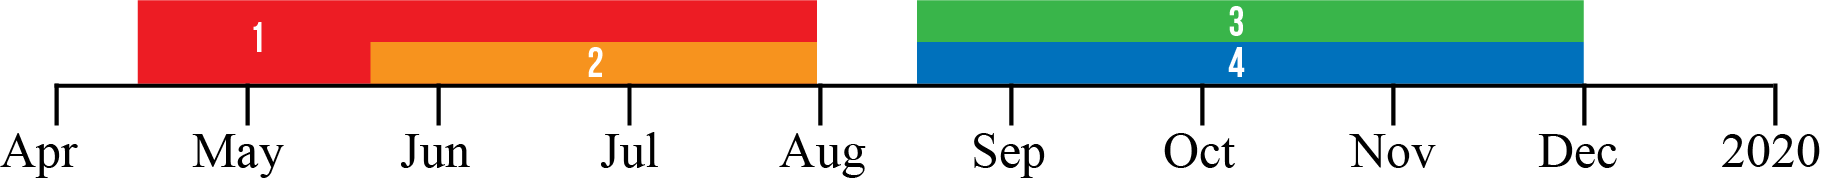
\includegraphics[width=\linewidth]{fig/Timeline.png}
\end{figure}

If the simulation of the patch sizes (2) will be so complicated such that after it cannot be completed before the end of July, we will drop objectives 3 and 4 and focus on the first two objectives. The deadline for the thesis is set to the end of November, such that a defense may be held in December.


%In the case that $p_{com} = 0$, the threshold for logical qubit recovery is $p_{loss} < 0.5$, which is equivalent to the \emph{bond percolation threshold}. In the case that $p_{loss} = 0$, computational errors can be found by measuring the stabilizer generators, which returns eigenvalue -1 on the edges of the error chains or syndromes, and can be corrected by finding a nontrivial closing chain, which either equals a stabilizer measurement that corrects the error, or a logical operator which equals a logical error. This problem is equivalent to the two dimensional random-bond Ising model (RBIM), where the shortest path needs to be found between matching pairs. The closing chain is found using the Edmonds' minimum weight perfect matching (MWPM) algorithm. In this case, the threshold is $p_{com} < 0.104$, for which a larger lattice size will decrease the chance of a logical error. These two thresholds corresponds to two end points of a boundary of correctability: $(p_{loss}, p_{comp}) = (0.5,0)$ and $(0,0.104)$.\\

%\subsubsection*{Superstabilizer decoder\cite{stace2009,stace2010}}
%To correct for losses on the surface code, new stabilizer generators are formed by connecting neighboring plaquettes or stars, which are connected to the same lost qubit, forming so-called superplaquettes and superstars respectively. These superstabilizers may share multiple qubits, and a nontrivial error chain arises of there are an odd number of (computational) errors in these shared qubits. This can be avoided by degrading the edges (shared qubits) between the superstabilizers to a single superedge whose error rates depend on the number of physical qubits shared, accounting for this degeneracy. For the sake of computation it is easier to stay on a square lattice. Take each stabilizer as a node and each shared qubit as an edge. The superstabilizer approach can be achieved by setting the weight of the edge of a lost qubit to 0, and the weight of shared edges between superstabilizers to the weight of the superedge. \\

%Using the superstabilizer approach, Edmonds' MWPM algorithm can be applied with altered edge weights. Simulations using the superstabilizers scheme with varying $p_{loss}$ show that the computational error threshold $p_{comp}^{thr}$ stay within the boundary of correctability, following the universal scaling law. At the limit of small $p_{loss}$, superstabilizer mostly consist of only 6 qubits, and increasing $p_{loss}$ only contributes to the number of superstabilizers, resulting in a linear relationship of threshold $p_{comp}^{thr}$ with $p_{loss}$.   As $p_{loss}$ increases further, larger superstabilizers containing more qubits appear, which have an increased chance of syndrome error. At $p_{loss} > 0.425$, the universal scaling law breaks down due to the size of the superstabilizers, as finite lattice effects dominate.\\

%One must also take into account that some error matchings may have a higher path degeneracy than others, indicating that the former is more likely. Therefore, the weights of the edges must additionally account for this degeneracy. However, due to this notion it possible that the algorithm may favor a matching that is not necessarily the shortest path. To balance these factors an additional factor $\tau$ is introduced that specifies the importance of path degeneracy. An optimal value for $\tau$ is found for which the computational error threshold is increased to $p_{comp}^{thr} = 0.1065$. Various implementations of Edmonds' MWPM algorithms are tested not to account for this degeneracy, and therefore a higher threshold may be possible with a computationally efficient algorithms that takes this into account.

%\subsubsection*{Maximum likelihood decoder\cite{delfosse2017}}
%Another way to look at erasure, is that the lost qubit is replaced by a maximally mixed state, which can also be interpreted as a qubit suffering a Pauli error $I,X,Y,Z$ chosen at random. Just as before, the decoding is done by measuring the plaquettes and stars, except now there is the additional knowledge of the erasure pattern, in which the errors must occur.\\

%For a set of errors $\sigma$ in the erasure pattern $\varepsilon$, either $X$ or $Z$ errors ($Y$ is a combination of the two), the algorithm is to make a spanning forest $F_{\varepsilon}$ inside of $\varepsilon$, a maximal subset of edges of $\varepsilon$ that contains no cycles. From this tree, boundary edges called leafs are iteratively stripped from $F_{\varepsilon}$. If the single connected vertex of the leave is in $\sigma$, the leaf or edge is added to the correction chain, and the other vertex is flipped in $\sigma$. What remains after the stripping $F_{\varepsilon}$ is the correction chain. On surface codes with boundaries, additional constrains are applied to the method of how the spanning forest is grown. \\

%\subsubsection*{Comparison}
%The benefit of the maximum likelihood decoder is that it scales linear with the size of the surface code. The spanning forest can be grown in linear-time, and the stripping process also only passes each leaf once, ensuring linear complexity. The superstabilizer decoder applies Edmonds' algorithm, which scales quadratic in time, but does however solve for erasure and computation errors simultaneously, whereas the maximum likelihood decoder only solves for erasure errors. Therefore, the optimal decoder probably depends on the size of the system.

  \chapter{Introduction}


Quantum computing has the potential to transcend the information technology as we know it. Small scale quantum systems are already possible today and the goal is to scale up these quantum architectures to build practical quantum devices. One approach to do this is to by networking many simple processor cells together through quantum links, avoiding the necessity to build a single complex structure. Processor cells that are located physically close to each other are connected by ``short'' links and lie in a patch. Patches that are located physically far from each other can in turn be connected by ``long'' links, such as remote optical connections. The total state of system, which contains the stored information, is shared across these patches, such that it can be accessed in either one of these patches. \\

This is somewhat analogous to the idea of a shared database. Many online services that we use today rely on servers that host the data that we want to view, store or edit. This data is often not stored on a single server, but copied to many others, in a shared database. In case one of these servers goes offline due to file corruption or an electricity outrage, the data is not lost, and can still be accessed on another server in the cluster.\\

In our Quantum network, information cannot be copied across different processor cells due to the no cloning theorem. In stead, it is shared across cells through entanglement. A cell can also go ``offline", when a qubit or multiple qubits are lost from the system due to some interaction with the environment. This process is called decoherence, also described with \emph{loss} or \emph{erasure}. Luckily, if the losses are not too much, these cells can be restored through quantum error correction (QEC) such that the quantum state or encoded information can still be extracted from the system. \\

\subsection{Quantum errors}
Errors that can occur during Quantum computation can generally be classified as 1) noise, in which there is an error are within the computational basis, or as 2) a loss, in which the qubit is
taken out of the computational basis. Losses are both detectable and locatable, which means that a higher rate of loss ($p_{loss}$) can be tolerated than noise or computational errors ($p_{com}$). The process of finding and correcting these errors is called decoding. \\

Kitaev's surfaces codes are defined by a set of stabilizers which act on a set of physical qubits that lie on the edges of a square lattice \cite{dennis2002topological}. The stabilizers commute, and are generated by plaquettes (group of $Z$ operators), or by stars (group of $X$ operators). Logical operates corresponds to a set of stabilizer operators along a homologically nontrivial cycle. Any homologically equivalent set of operators can be used to measure the physical qubit operator. Therefore, in the case of a qubit loss, another set of operators can be used, if there is no \emph{percolated} region of losses that span the entire lattice. \\

To decode for computational errors, one measures the stabilizer generators, which returns eigenvalue -1 on the edges of the error chains or syndromes, and can be corrected by finding a nontrivial closing chain, which either equals a stabilizer measurement that corrects the error, or a logical operator which equals a logical error. This problem is equivalent to the two dimensional random-bond Ising model (RBIM), where the shortest path needs to be found between matching pairs. The closing chain is found using the Edmonds' minimum weight perfect matching (MWPM) algorithm. This algorithm scales quadratic in time as the lattice size increases \cite{stace2009thresholds}. More recently, an almost-linear decoding approach has been described by Delfosse et al. \cite{delfosse2017linear}. \\

There are also multiple methods to decode for losses on the surface code. Stace et. al \cite{stace2009thresholds,stace2010error} describes the method of so-called superplaquettes and superstars, in which the lost qubit is accounted for by combining neighboring stabilizers. The resulting lattice can be than decoded using the same MWPM algorithm. Delfosse et al \cite{delfosse2017linear} describes a linear-time maximum likelihood method to decode for losses. Here, the errors are found in a \emph{peeling} algorithm that iteratively peels branches away from a tree of possible error chains until the lost qubits remain.

The Union-Find decoder is preferred over other types of decoders because it is \emph{simple}. Even though it may not seem so due to the length of its chapter, the concept of the Union-Find decoder is much more straightforward compared with other, more advanced decoders. 


Chapters \ref{ch:qec} up until Chapter \ref{ch:UFdecoder} Section \ref{sec:bucketwg} are descriptions of existing and known material. Section \ref{sec:bucketwg} and onwards includes exclusively our own contributions. 
  \chapter*{Notations}
\addcontentsline{toc}{chapter}{Notations}
In this chapter, we introduce the notations that we will be using throughout this thesis. With the defined notations, we also list the symbols used in this thesis. 

\paragraph{Quantum operator}
\begin{itemize}[leftmargin=4em, align=left]
    \item[$\hat{X}$]  Hatted symbols denote quantum operators on a quantum state.
\end{itemize}

\paragraph{Sets, lists, and groups}
\begin{itemize}[leftmargin=4em, align=left]
    \item[$\m{X}$]  Calligraphic symbols denote some set  or list of elements of the some type, or groups. 
\end{itemize}

\paragraph{Functions on sets}
\begin{itemize}[leftmargin=4em, align=left]
    \item[$\n{X}$]  Scripted symbols denote some function on a set, that has a set with elements of a different type as output. Set functions exists only to simplify notations. 
\end{itemize}

\paragraph{Algorithms}
\begin{itemize}[leftmargin=4em, align=left]
    \item[\codefunc{AlgorithmX}] Capitalized mono-spaced refer to some applied function or algorithm. 
\end{itemize}

\paragraph{Object-attribute notation}
\begin{itemize}[leftmargin=4em, align=left]
    \item[$x.var$]  Symbols with $.$ in between denote some attribute $var$ stored at the object $x$.
\end{itemize}
\emph{In this thesis, we will use simulated results to benchmark and compare the performance for several types of decoders for the surface code. These simulations are performed using our own simulation package (see Appendix \ref{ap:oopsurfacecode}), which utilizes an object-oriented programming structure. In this structure, instances of an object, which is equivalent to elements of some set, have attributes that are stored at the object instance.}

\paragraph{Others}
\begin{itemize}[leftmargin=4em, align=left]
    \item[$(u,v)$]  Edges of a graph can be denoted with the vertices $u,v$ that supports it.
    \item[$\tilde{X}$]  Refers to some instance of $X$, e.g. $\tilde{\m{X}}$ denotes some set $\m{X}$. 
    \item[$\m{O}$] Big O notation for describing the limiting behavior of a function when the argument increases in size. 
\end{itemize}




% In this chapter, we will present an object-oriented implementation of surface code simulations. The goal of this chapter is not to describe in detail the classes and methods used for these simulations, but mainly introduce the notion of object attributes. In the remainder of the thesis, we will often refer to variables that are stored \emph{at} some physical entity, with which we mean that the variable is stored as an attribute at the class instance of that entity. 



  \chapter{Quantum error correction}

To build a real world quantum computer, or a quantum communications device, one has to deal with the presence of noise, which will inevitably alter the quantum state of a qubit stored or passed through a communications channel. Recent developments have raised the fidelity of single qubit operations to up to one single failure in $10^6$ operations \cite{ballance2016high}. But even this fidelity is not enough, as a full quantum computation may require millions of qubits, and the generation of entangled states over a large number of qubits. With imperfect quantum gates, anything we do in order to perform a computation will add to the error. 

The theory of \emph{quantum error correction} has been developed to counteract this noise, by using a larger number of redundant \emph{physical qubits} to encode for a smaller number of \emph{logical qubits}. By adding extra redundant qubits in our \emph{error correcting code}, we can carefully encode the quantum state which we wish to protect, as long as the rate of errors on the physical errors is low enough \cite{calderbank1996good, steane1996multiple, preskill1998reliable}.

In this chapter, we will introduce the principles of quantum error correction by the example of the \emph{three-bit repetition code}. In section \ref{sec:classical3bit}, we will first cover the classical variant, and the quantum variant in section \ref{sec:quantum3bit}. A more practical language to describe these codes is the \emph{stabilizer formalism}, in section \ref{sec:stabilizerformalism}. The set of tools and principles explained in these sections form the basis for higher level quantum codes that we will come later in this thesis.

\section{Classical three-bit repetition code}\label{sec:classical3bit}
To introduce some of the terms that we are going to use later, let us first start with a classical example the three-bit repetition code. This code encodes bits (a single bit in the example) by repeating them. Let the \emph{codewords} of the single logical bit be:
\begin{align}\label{eq:qb_3bitlogical}
    && 0_L = 000 &&& 1_L=111 &
\end{align}
In order to do computations, a NOT gate may be applied to the codewords to flip the logical value:
\begin{equation}
 000 \leftrightarrow 111
\end{equation}
A \emph{bit-flip} error can occur on any of the three bits in the code, which flips the single bit-value from 0 to 1 and 1 to 0. An error can be \emph{detected} by measuring the bits and comparing whether the bits have equal value. An detected error can be \emph{corrected} by computing the majority-function of the bitstring. Thus the three-bit repetition code will be correctly corrected if less than half of the bits were flipped.
\begin{align}
  0_L \xrightarrow{E_2} 010 \xrightarrow{correction} 000 && 0_L \xrightarrow{E_2, E_3} 011 \xrightarrow{correction} 111
\end{align}
The \emph{distance} $d$ of a classical code is the minimum amount of bit flips to transfer one codeword to another. In the case of the three-bit repetition code, the code distance is 3. The number of bits in de code $n$, the number of encoded bits $k$ and the distance of a code can be used to fully describe a code in the $[n, k, d]$ notation. The three-bit repetition code is a $[3,1,3]$ code.

\section{Quantum three-bit repetition code}\label{sec:quantum3bit}

From here, we can describe how to do computations on a quantum system. We start by considering an example of the \emph{quantum three-bit repetition code}, where the classical bits are now replaced by qubits that can be in the superposition of the two classical 0 or 1 states. The basis states of the encoded qubit is the tensor product of the single qubit states:
\begin{align}\label{eq:qb_3bitlogicalq}
&& \ket{0}_L = \ket{0}\otimes\ket{0}\otimes\ket{0} = \ket{000} && \ket{1}_L = \ket{1}\otimes\ket{1}\otimes\ket{1} = \ket{111}
\end{align}
A pure qubit state can also be a superposition of the bases states and is encoded as:
\begin{equation}\label{eq:qec_3bitstate}
  \ket{\psi}_L = \alpha\ket{0}_L + \beta\ket{1}_L
\end{equation}

\subsection{Pauli operators}\label{subsec:pauli}

The Pauli operations are unitary operations on single qubits, and will be applied very often throughout this thesis. Including the identity operator, the Pauli group on a single qubit, $\gls{pauligroup}_1$, consists of:
\begin{align}
  \gls{X} = \begin{bmatrix} 0 & 1 \\ 1 & 0 \end{bmatrix} &&
  \gls{Y} = \begin{bmatrix} 0 & -i \\ i & 0 \end{bmatrix} &&
  \gls{Z} = \begin{bmatrix} 1 & 0 \\ 0 & -1 \end{bmatrix} &&
  \gls{I} = \begin{bmatrix} 1 & 0 \\ 0 & 1 \end{bmatrix}
\end{align}
The Pauli operators represent errors that can occur on a single qubit. The Pauli X operator is analogous to the classical \emph{bit-flip} error and acts on the qubit computational basis states:
\begin{align}\label{eqq:qec_bitflip}
  & X\ket{0} = \ket{1} && X\ket{1} = \ket{0} &
\end{align}
Additionally, the Pauli Z operator introduces phase errors on a quantum bit:
\begin{align}\label{eq:eqc_phaseflip}
  & Z\ket{0} = -\ket{0} && Z\ket{1} = -\ket{1} &
\end{align}
The elements of the Pauli group on $n$ qubits, $\m{P}_n$, consists of tensor products of single qubit Pauli operators, such that  $\m{P}_n = \m{P}_1^{\otimes n}$. We use the index of a Pauli operator to indicated on which qubit it has operated on, while other qubits are acted on by the identify. In cases without indices, the order of the operators indicate the qubit it acts on. For example, element $P=X_1\otimes X_2 = XX$ on the three-bit repetition code means that qubit 1 and 2 have been acted on by the Pauli X operator, while qubit 3 is acted on by the identity. The tensor product symbol is often omitted for clarity, such that the above operation can be also written as  $P=X_1X_2$. The \emph{weight} of an operator is the number of qubits on which it does not act non-trivially. On the pure  three-qubit encoded state, a bit-flip error on the second qubit is applied as:
\begin{equation}\label{eq:qec_3bitflip}
  X_2\ket{\psi}_L = (I\otimes X \otimes I) \ket{\psi}_L = \alpha\ket{010} + \beta\ket{101}
\end{equation}

\subsection{Logical operations}

In order to do computations on the encoded qubit of our three-bit repetition code, we wish to find the Pauli operators in $\m{P}_3$ which flips any basis of the basis states of the encoded qubit to the other. We find that $X\otimes X\otimes X$ transforms $\ket{0}_L$ to $\ket{1}_L$, which is known as the logical bit-flip.

Furthermore, we now have the logical Z operator which must map $\ket{0}_L$ to $-\ket{0}_L$ and $\ket{1}_L$ to $-\ket{1}_L$. We see that for example $Z\otimes I\otimes I$ achieves this, but also any other $\m{P}_3$ operator with two identities and one Pauli Z operator. Thus there are multiple operators that achieves the same. We formalize the logical operators as
\begin{align}\label{eq:qec_3bitlogical}
  \gls{Xlogical} = XXX && \gls{Zlogical} = ZII
\end{align}

The distance of a quantum code is the minimal weight of any logical operators on the code. In the above case, the weight of the encoded X operator $\bar{X}$ is 3, hence the code can detect up to 2 X errors, analogous to the classical case. However, the weight of the encoded Z operator $\bar{Z}$ is only 1, which means that Z errors cannot be detected at all.

\subsection{Error detection}

To detect errors in our repetition code, we now cannot measure the states directly, as any measurement would collapse the encoded state, and therefore destroy the encoded information. Instead, we can now detect errors by measuring the \emph{parity} of two or more qubits rather than single qubits. For example, for two qubits, we can measure the parity by adding an \emph{ancillary} or \emph{ancilla} qubit prepared in $\ket{0}$ and measure it in the computational basis after connecting our quantum circuit as:

\begin{figure}
  \centering
    \begin{tikzcd}[row sep={0.65cm,between origins}]
    \lstick{$Q_1$} & \qw & \ctrl{2} & \qw & \qw &\\
    \lstick{$Q_2$} & \qw & \qw & \ctrl{1} & \qw &\\
    \lstick{$\ket{0}$} & \qw & \targ{} & \targ{} & \qw & \meter{}
  \end{tikzcd}
  \caption{The quantum circuit for a parity measurement on two qubits, $Q_1$ and $Q_2$, which is measured on the ancilla qubit prepared in $\ket{0}$. }\label{fig:2qubitparity}
\end{figure}


Note that measuring the ancilla qubit in the computational basis will be equivalent to measuring $Z\otimes Z$ on the first two qubits, as
\begin{equation}
\begin{aligned}
    (ZZ)\ket{00} &= \ket{00} && (ZZ)\ket{01} &= -\ket{01} \\
    (ZZ)\ket{10} &= -\ket{10} && (ZZ)\ket{11} &= \ket{11}
\end{aligned}
\end{equation}
Now for our quantum three-bit repetition code, we need to setup ancilla qubits between each of the 3 qubits, such that the parity between any two qubits can be measured. For the state in equation \ref{eq:qec_3bitstate}, any parity measurement $ZZI$, $ZIZ$ or $IZZ$ will return even parity. If one of the qubits has encountered a bit-flip error such as in the second qubit in equation \ref{eq:qec_3bitflip}, two of the parity measurements will return a -1 eigenvalue, in this case $ZZI$ and $IZZ$.

Furthermore, we see that no configuration of ancilla qubits could be set up for the three-bit repetition code to detect for phase errors, which was already set by the weight of the logical Z operator.

\subsection{Error correction}

As the error has been identified, we can apply correct Pauli operator from $\m{P}_3$ to correct the error. In the above case, we wish to apply $IXI$ to clip the second qubit to correct the code.

In the quantum three-bit repetition code, we can very simply deduct which qubit has encountered an error from the combination of uneven parity measurements. This is called \emph{decoding} the error and is the main function of a \emph{decoder}. More complex error correcting codes involves decoding algorithms which are far more complex than in the three-bit repetition code, which we will see more of later.


\section{Stabilizer Formalism}\label{sec:stabilizerformalism}

As we have seen above, we can use the Pauli group $\m{P}_n$ to easily describe a quantum error correcting code of $n$ qubits, without explicitly looking at the \emph{state} of the qubit. This powerful technique is called the \emph{stabilizer formalism} \cite{gottesman1997stabilizer}, and is the most widely formalism used to describe topological codes.

A quantum error correcting code that can be described using the stabilizer formalism is called a \emph{stabilizer code}. A stabilizer code is defined by two sets of operators: 1) a set of \emph{stabilizer generators} $\gls{stabilizergenerator}$ which generates the \emph{stabilizer group} $\gls{stabilizergroup}$, an Abelian subgroup of the Pauli group, and 2) a set of encoded \emph{logical operators}. A stabilizer group is the set of Pauli operators which leave all states $\ket{\psi}_i$ from the \emph{codespace}, a subspace of the Hilbert space of $n$ qubits spanned by the codeword basis states, invariant, such that
\begin{align}
  & \gls{stabilizer}\ket{\psi}_i = \ket{\psi}_i, && \forall S \in \m{S}. &
\end{align}
The elements of the of the stabilizer group $S\in\m{S}$ are most simply referred to as \emph{stabilizers}. Any stabilizer $S$ can be written as a product of elements from a set of stabilizer generators $\mathfrak{s}=\{s_1,...,s_{N_s}\}$.  
\begin{align}
 & S = \prod_{j=1}^{N_s}s_j^{a_j}, && a_j \in {0, 1} &
\end{align}
The set of stabilizer generators $\mathfrak{s}$ is \emph{independent} if no generator can be written as a product of other generators. This implies that any stabilizer can be written in terms of the bitstring $a_1, a_2, ...a_{N_s}$ and that the stabilizer group takes up $N_s$ degrees of freedom of the Hilbert space of $N$ qubits. The remaining $N-N_s = N_l$ degrees of freedom which are not specified by the stabilizers make up the \emph{codespace}, the subspace spanned by the logical basis states, or the number of encoded logical qubits. Thus, if $N_l$ logical qubits are to be encoded by $N$ qubits, we require a total of $N_s = N-N_l$ independent stabilizer generators.


\subsection{Encoded logical operators}

Next to the set of stabilizers, we can construct the set of logical operators that will act on the encoded qubits from a set commutation rules. First of all, all logical operators must commute with all elements of the stabilizers, as a logical operator is made up from Pauli operators, and any Pauli operator which anticommutes with a stabilizer cannot leave the codespace invariant. Note that his means that a logical operator is not unique, as it can be multiplied with an element of the stabilizer. Secondly, we can impose commutation rules for the logical operators themselves based on the Pauli operators that they are representing. For example, logical $\bar{X}$ and $\bar{Z}$ operators must anticommute.

The minimum weight of the logical operator determines the distance $d$ of the error correcting code. This is thus the minimal amount of errors that can cause a logical failure. Together with the total number of qubits $n$ and number of logical qubits $k$, they provide a rough measure of the error correcting capabilities of the code.

\subsection{Error detection procedure}

As the stabilizers are a set of Pauli operators, they correspond to blip-flip or phase-flip errors that may have happened on any of our $n$ qubits. Furthermore, as any stabilizer leaves all states  $\ket{\psi}_i$ invariant, measuring the stabilizers does not disrupt the encoded information. If no error has occurred, all stabilizer measurements will return a '+1' eigenvalue, while any '-1' outcome points to the presence of errors, which we will call a \emph{stabilizer violation}.

This outcome is dependent on whether an error caused by the error operator $\gls{perror}$, must either commute or anticommute with the stabilizer generators, since all operators are members of the same Pauli group $\m{P}_n$. If $P$ and generator $s$ commute then,
\begin{equation}
  sP\ket{\psi} = Ps\ket{\psi} = P\ket{\psi}
\end{equation}
which means that the post-error state is a +1 eigenstate of $S_j$. If $O$ and generator $S_j$ anticommute then,
\begin{equation}\label{qec:eq:stabmeas}
  sP\ket{\psi} = -Ps\ket{\psi} = -P\ket{\psi}
\end{equation}
and the post-error state is a -1 eigenstate of $s$. Errors on stabilizers codes are therefore detected by measuring the stabilizers, which returns a series of eigenvalue outcomes that is called the \emph{syndrome}. However, it is not necessary to measure all operators in the stabilizer group $\m{S}$. Measuring the set of independent stabilizer generators $\mathfrak{s}=\{s_1,...,s_{N_s}\}$ suffices as any other stabilizer is just a combination of already measured states.

\subsection{Error models}\label{qec:sec_errormodels}

Any qubit can be subject to a combination of errors, each can be caused by a difference factor in our quantum system. To generalize these errors, we define certain \emph{error models} that constricts the errors that take place. Here, we list a few models that we will encounter in this thesis. 

\paragraph{Independent noise model}
We were already introduced in the \emph{bit-flip} and \emph{phase-flip} errors in section \ref{subsec:pauli}. But let us know generalized them in the form of the density matrix $\rho$. Let $\Phi$ be a quantum channel that maps $\rho$ to $\Phi(\rho)$, and let the chance of a bit-flip error be $p_X$, the resulting state should be
\begin{equation}\label{qec:eq:bitflip}
  \Phi_X(\rho) = (1-p_X)\rho + p_X(X\rho X).
\end{equation}
Analogously, let the chance of a phase-flip error be $p_Z$, the resulting state should be
\begin{equation}\label{qec:eq:phaseflip}
  \Phi_Z(\rho) = (1-p_Z)\rho + p_Z(Z\rho Z).
\end{equation}

The bit-flip and phase-flip errors can be considered together as the \emph{independent noise model} or the \emph{uncorrelated noise model}. As the two types of errors are independent, they can be studied separately from each other.

\paragraph{The depolarizing noise model}
In the \emph{depolarizing} noise model, the afflicted quantum state is replaced by a complete mixed state with probability $p_D$. Let the completely mixed state be written as
\begin{equation}\label{qec:eq:mixstate}
  \frac{1}{2}I = \frac{1}{4}(\rho + X\rho X + Y\rho Y + Z\rho Z),
\end{equation}
then the depolarizing channel is described as
\begin{align}\label{qec:eq:depolarizing}
  \nonumber \Phi_D(\rho) &= (1-p_D)\rho + p_D\left(\frac{1}{2}I\right) \\
  \nonumber &= \left(1-\frac{3}{4}p_D\right)\rho + \frac{p_D}{4}(X\rho X + Y\rho Y + Z\rho Z) \\
  &= (1-p^*_D)\rho + \frac{p^*_D}{3}(X\rho X + Y\rho Y + Z\rho Z),
\end{align}
which can be interpreted as the state $\rho$ is left untouched with probability $p^*_D =\frac{3}{4}p_D$, and each Pauli gate is applied to it with probability $1-p^*_D$. Differently from the \emph{independent noise model}, to optimally decode, we need to take into account correlations between X and Z errors.

\paragraph{The erasure noise model}
In the \emph{erasure} noise model, a qubit is completely erased or lost from the system,
\begin{equation}\label{qec:eq:erasure}
  \Phi_E(\rho) = (1-p_E)\rho + p_E\ket{e}\bra{e},
\end{equation}
where the state $\ket{e}$ is outside the qubit space. Such a loss can be detected and the missing qubit is then replaced by a qubit in the totally mixed state (equation \ref{qec:eq:mixstate}). The erasure channel can therefore be seen as the depolarizing channel with the extra property that it can be detected which qubits suffer the error.


\subsection{Error correction or decoding}

As the Pauli operators are self-inverse, any error $E$ can be corrected by applying it again. From the measurement outcomes of a stabilizer measurement, we can deduce which error $E$ must have caused the syndrome. However, this relationship is not always one-to-one, as an error $E$ and its multiplication with a stabilizer $ES$ will lead to an identical syndrome. This is called the \emph{code degeneracy}. The choice of the most appropriate error to correct is not a trivial task, and algorithms that are tasked to automate this process are called \emph{decoders}.

\subsection{Stabilizer codes}

The three-qubit repetition code we already covered can now be described in the stabilizer formalism. We had already found that the logical operators are encoded $\bar{X} = XXX$ and $\bar{Z} = ZII$. Other logical operators also exist up to a stabilizer. The stabilizer generators are needed to complete its description. We had found that two parity measurements, for example $ZZI$ and $IZZ$, will identify the error, as they will either commute or anticommute with the error, as such they are a set of independent stabilizer generators. 

The resulting measurement of '+1' or '-1' eigenvalues make up the syndrome. De decoder algorithm here is quite simple, but fails in the case if there is more than 1 bit-flip error. The code has $n=3$ and $n_S=2$ which results in the expected $n_L = 1$ encoded bits. The distance $d$ of the is 1, which conforms that there are certain errors, in this case phase-flip errors, which this code cannot detect.

The smallest code which can correctly solve for both single bit-flip and phase-flip errors is the \emph{5-qubit repetition code} \cite{laflamme1996perfect}. This code has the following stabilizer generators:
\begin{align}
  XZZXI && IXZZX && XIXZZ && ZXIXZ
\end{align}
with the logical operators up to a stabilizer:
\begin{align}
  & \bar{X} = XXXXX && \bar{Z} = ZIIII &
\end{align}
This codes now has $n=5$ bits with $n_S = 4$ stabilizers, which means it still encodes for a single bit.\\
\\
\\
With the principles of encoding and decoding in the quantum error correction in mind, we are now ready to move on to a more complicated variant of stabilizer codes, the \emph{surface code}. 



  
\chapter{The surface code}

The variant of the stabilizer codes that we are going to explore in this thesis is Kitaev's \emph{surface code} \cite{kitaev2003fault}, which is of the category of \emph{topological codes}. Among this category, the surface code is preferable as it offers the highest error tolerance under realise noise channels and requires only local stabilizer measurements of physically neighboring qubits. Two variants of the surface code will be considered here, the \emph{toric code} in section \ref{sec:surface_toric} and the \emph{planar code} in section \ref{sec:surface_planar}, and various decoders are detailed in \ref{sec:surface_decoders}.
\begin{figure}
  \centering
  \begin{tikzpicture}[scale=0.8]
    \DRAWTORIC{3}
    \draw [arrow] (-1,0 |- N-0-2-1) node [align=right, left] {qubit/edge} -- (N-0-2-1);
    \node (plaquette) at ($(N-0-1-0)!0.5!(N-0-0-0)$) {};
    \node (star) at ($(N-1-0-1)!0.5!(N-1-1-1)$) {};
    \draw [arrow] (-1,0 |- plaquette)  node [align=right, left] {face} -- (plaquette);
    \draw [arrow] (-1,0 |- N-1-0-1) node [align=right, left] {vertex} to [out=0, in=225] (star);
    \node [align=left, right] at (3*\s + .5, .5*\s) {periodic boundary};

  \end{tikzpicture}
  \caption{The toric code is defined as a $L\times L$ lattice (here $L=3$) with periodic boundary conditions. The edges on the lattice, which represents the qubits, make up faces and vertices. (Figure inspired from \cite{browne})}\label{sf:fig_toriclattice}
\end{figure}

\section{The toric code}\label{sec:surface_toric}
The \emph{toric code} is defined by arranging qubits on the edges of a square lattice with periodic boundary conditions, as seen in Figure \ref{sf:fig_toriclattice}. The name of the toric code lends itself from the torus, or donut, shape, where any point on the surface of the torus will encounter itself after traversing the torus in either x or y directions. Hence, the top edge of the toric code meets the bottom edge, whereas the left edge meets the right. On a $L\times L$ grid there are $N = 2L^2$ edges and the same amount of physical qubits. This topology of qubit arrangement plays an important part in encoding the logical qubits, which is stored in the non-trivial cycles on the torus. Errors, beneath a certain threshold, will only introduce local effects and does not change these cycles.

\subsection{Stabilizer generators}

To define a stabilizer code, we need to specify the $m$ independent stabilizer generators and the encoded $\bar{X}$ and $\bar{Z}$ operators. On the toric code there are two types of stabilizer generators, \emph{plaquette} and \emph{star} operators, which are associated with the \emph{faces} and \emph{vertices} of the square lattice, respectively.

\begin{figure}
  \centering
  \begin{tikzpicture}
    \DRAWTORIC{3}
    \DRAWPLAQ{1}{1}
    \DRAWERROR{1}{1}{0}{z}
    \DRAWERROR{1}{1}{1}{z}
    \DRAWERROR{1}{0}{0}{z}
    \DRAWERROR{2}{1}{1}{z}
    \node[below of=Bx-1] {(a)};
  \end{tikzpicture}
  \hspace{1cm}
  \begin{tikzpicture}
    \DRAWTORIC{3}
    \DRAWSTAR{1}{1}{3}
    \DRAWERROR{1}{1}{1}{x}
    \DRAWERROR{1}{1}{0}{x}
    \DRAWERROR{1}{2}{1}{x}
    \DRAWERROR{0}{1}{0}{x}
    \node[below of=Bx-1] {(b)};
  \end{tikzpicture}

  \begin{center}
    \hspace{1cm}
    \begin{tikzcd}[row sep={0.5cm,between origins}]
      \lstick{$Q_1$} & \qw & \qw & \qw & \ctrl{5} & \qw \\
      \lstick{$Q_2$}& \qw & \qw & \ctrl{4} & \qw & \qw \\
      \lstick{$Q_3$} & \qw & \ctrl{3} & \qw & \qw & \qw \\
      \lstick{$Q_4$} & \ctrl{2} & \qw & \qw & \qw & \qw \\
      &&&&&&&\\
      \lstick{$P_f$} & \ctrl{} & \ctrl{} & \ctrl{} & \ctrl{} & \meter{}
    \end{tikzcd}
    \begin{tikzcd}[row sep={0.5cm,between origins}]
      \lstick{$Q_1$} & \qw & \qw & \qw & \targ{} & \qw \\
      \lstick{$Q_2$} & \qw & \qw & \targ{} & \qw & \qw \\
      \lstick{$Q_3$} & \qw & \targ{} & \qw & \qw & \qw \\
      \lstick{$Q_4$} & \targ{} & \qw & \qw & \qw & \qw \\
      &&&&&&&\\
      \lstick{$S_v$} & \ctrl{-2} & \ctrl{-3} & \ctrl{-4} & \ctrl{-5} & \meter{}
    \end{tikzcd}
  \end{center}

  \caption{Each face (a) and vertex (b) on the lattice represents a plaquette and star operator, respectively. The non-identity single qubit operators on which they act are indicated. The set of all (but one) plaquettes and vertices make up the stabilizers of the code. (Figure inspired by \cite{browne})}\label{sf:fig_stabilizers}
\end{figure}

\paragraph{Plaquette operators}
For every face $f$ on our lattice, we define a plaquette operator $P_f$, consisting of tensor product of Pauli Z operators on qubits on these edges (see Figure \ref{sf:fig_toriclattice}a),
\begin{equation}\label{eq:sf_plaquette}
  \gls{plaquette} = \prod_{i\in Q(f)} Z_i
\end{equation}
where $Q(f)$ is the set of qubits touching face $f$. On a $L\times L$ grid there are $L^2$ plaquettes.

\paragraph{Star operators}
Similarly, for every vertex $v$ on our lattice, we define a star operator $S_v$, consisting of tensor product of Pauli X operators on qubits neighboring the vertex (see Figure \ref{sf:fig_toriclattice}b),
\begin{equation}\label{eq:sf_star}
  \gls{star} = \prod_{i\in Q(v)} X_i
\end{equation}
where $Q(v)$ is the set of qubits neighboring vertex $v$. On a $L\times L$ grid there are $L^2$ plaquettes.

As each plaquette and star operator needs to be measured, an ancilla qubit is needed at the physical locations of each of these operators. The structure of the full lattice is now clear, as it just a simple square arrangement of alternating data and ancilla qubits in both x and y directions.

The full stabilizer of the code $\m{S}$ can be generated by multiplying elements of the generator operators. Consider two plaquette operators. These two operators will either share one boundary consisting of a qubit, or none. This means that the Pauli Z operator on the boundary qubit will add up to identity as they commute. The result is that the product of the plaquette operators will consists of the overall boundary Pauli operators of the joint plaquette (see Figure \ref{sf:fig_multistab}a).

However, if all plaquettes are applied to the lattice, no boundary will be left. Thus the product of all plaquettes is the identity, which means that the full set of plaquettes are not independent. The full set of plaquette generators can therefore be completed by simply removing a single plaquette from all available plaquettes. There are therefore $L^2 - 1$ independent plaquette operators.

The multiplication of star operators follow the same properties as the plaquette operators described above (see Figure \ref{sf:fig_multistab}b). Thus there are also $L^2 - 1$ independent star operators, which are the star generators. This sums up to $N_S = 2L^2 - 2$ independent stabilizer generators.

\begin{figure}
  \centering
  \begin{tikzpicture}
    \DRAWTORIC{3}
    \DRAWPLAQ{1}{1}
    \DRAWPLAQ{0}{1}
    \DRAWPLAQ{0}{2}
    \DRAWERROR{1}{1}{0}{z}
    \DRAWERROR{1}{0}{0}{z}
    \DRAWERROR{2}{1}{1}{z}
    \DRAWERROR{0}{0}{0}{z}
    \DRAWERROR{0}{1}{1}{z}
    \DRAWERROR{0}{2}{1}{z}
    \DRAWERROR{0}{2}{0}{z}
    \DRAWERROR{1}{2}{1}{z}
    \node[below of=Bx-1] {(a)};
  \end{tikzpicture}
  \hspace{1cm}
  \begin{tikzpicture}
    \DRAWTORIC{3}
    \DRAWSTAR{1}{1}{3}
    \DRAWSTAR{2}{0}{3}
    \DRAWSTAR{2}{1}{3}
    \DRAWERROR{1}{2}{1}{x}
    \DRAWERROR{0}{1}{0}{x}
    \DRAWERROR{2}{2}{1}{x}
    \DRAWERROR{1}{1}{1}{x}
    \DRAWERROR{1}{0}{0}{x}
    \DRAWERROR{2}{0}{1}{x}
    \DRAWERROR{2}{0}{0}{x}
    \DRAWERROR{2}{1}{0}{x}
    \node[below of=Bx-1] {(b)};
  \end{tikzpicture}
  \caption{Multiplication of (a) plaquette and (b) star operators will result in a operator that consists of the Pauli operators that reside on the overall boundary of the joint plaquettes or stars. (Figure inspired by \cite{browne})}\label{sf:fig_multistab}
\end{figure}

\subsection{Dual lattice}
Note that if we shift our lattice half a cell down, and half a cell to the right, we can create a \emph{dual} lattice. This dual lattice has the same size and same boundary conditions as the \emph{primal} lattice, but every plaquette in the primal lattice is a star in the dual lattice, and every star in the primal lattice is a plaquette in the dual lattice. The edges of the dual lattice are plotted with dotted lines in the figures.

This interesting property of \emph{lattice duality} leads to the fact that plaquette and star operators are in fact the same, and we can choose from either that is best suited for the calculation. The multiplication of operators is best pictured in the plaquette picture, for example. For the square lattice in the toric code, the dual lattice is coincidentally also square. For other types of topological codes with non-square lattices, the dual lattice has a different lattice structure than the primal lattice. We will not explore these kind of lattices in this thesis.

\subsection{Encoded qubits}
Since there are $N = L^2$ qubits and $N_S = 2L^2 - 2$ independent stabilizers, we must have $N_L = N - N_S = 2$ encoded qubits and therefore 4 logical operators $\bar{X}_1, \bar{X}_2, \bar{Z}_1$ and $\bar{Z}_2$.

Recall the logical operators consists of the Pauli operators, and must commute with all stabilizer generators, but cannot be part of the stabilizer itself. We can construct the logical operators by starting with, for example, a single Pauli Z operator. It commutes with all plaquette operators trivially. In terms of the star operators, this single Pauli Z operator commutes with all but the two neighboring qubits, as all others apply to different qubits. Adding another Pauli Z operator will shift will of the anticommuting neighboring star operators. We know see that a closed loop of Z operators around the torus does not have neighboring star operators, and therefore commute with all stabilizers. As the torus has two directions we can loop over, these are the logical $\bar{Z}$ operators (see Figure \ref{sf:fig_logical}a-b). Analogously, we can construct the logical $\bar{X}$ operators in the same way (Figure \ref{sf:fig_logical}c-d).

Note that these logical operators are not unique. As the logical operators commute with the stabilizers, these $\bar{X}$ and $\bar{Z}$ operators can be multiplied with e.g. a plaquette or star operator, respectively, which create a diversion from its original path. But as the path still loops around the torus, this is still a valid logical operator.

The logical operators have a minimum length of $L$ qubits, which is also the distance of the toric code. The toric code is therefore a $[L^2,2,L]$ in the [n,k,d] notation. This implies that the toric code might be more robust against errors if the size of the lattice is increased. Later we will see that this is also very much dependent on the type of decoder that is used, and that different decoders will lead to different regimes of error for which this reasoning is true.

\def\QS{10}
\def\s{1}

\begin{figure}
  \centering
  \begin{tikzpicture}
    \DRAWTORIC{5}
    \DRAWERROR{0}{2}{0}{z}
    \DRAWERROR{1}{2}{0}{z}
    \DRAWERROR{2}{2}{0}{z}
    \DRAWERROR{3}{2}{0}{z}
    \DRAWERROR{4}{2}{0}{z}
    \DRAWERROR{3}{0}{1}{z}
    \DRAWERROR{3}{1}{1}{z}
    \DRAWERROR{3}{2}{1}{z}
    \DRAWERROR{3}{3}{1}{z}
    \DRAWERROR{3}{4}{1}{z}
    \begin{pgfonlayer}{edges}
      \draw[synz] (S-0-2) -- (S-5-2);
      \draw[synz] (S-3-4) -- (S-3-5);
    \end{pgfonlayer}
    \node[above=.25cm of S-3-4] {(a)};
    \node[left=.25cm of S-0-2] {(b)};
  \end{tikzpicture}
  \hspace{1cm}
  \begin{tikzpicture}
    \DRAWTORIC{5}
    \DRAWERROR{0}{2}{1}{x}
    \DRAWERROR{1}{2}{1}{x}
    \DRAWERROR{2}{2}{1}{x}
    \DRAWERROR{3}{2}{1}{x}
    \DRAWERROR{4}{2}{1}{x}
    \DRAWERROR{3}{0}{0}{x}
    \DRAWERROR{3}{1}{0}{x}
    \DRAWERROR{3}{2}{0}{x}
    \DRAWERROR{3}{3}{0}{x}
    \DRAWERROR{3}{4}{0}{x}
    \begin{pgfonlayer}{edges}
      \draw[synx] (N-0-2-1) -- (By-2);
      \draw[synx] (Bx-3) -- (N-3-4-0);
    \end{pgfonlayer}
    \node[above=.25cm of N-3-4-0] {(c)};
    \node[right=.25cm of By-2] {(d)};
  \end{tikzpicture}
  \caption{The logical (a) $\bar{X}_1$, (b) $\bar{X}_2$, (c) $\bar{Z}_1$ and (d) $\bar{Z}_2$ operators are the closed loop of $X$ and $Z$ operators, respectively, that go around the two boundaries of the torus. (Figure inspired by \cite{browne})}\label{sf:fig_logical}
\end{figure}

\subsection{Error detection}
As discussed in the previous chapter, errors are detected by measuring the set of stabilizer generators. As we have seen in the previous section, this consists of all but one plaquette operators $P_f$ and all but one star operators $S_v$. Let us first consider to measure all of them.

In the case of a single $Z$ error (Fig \ref{sf:fig_degenerate}a.i), the neighboring plaquette operators will commute with this error, as it consists of Pauli Z operators itself. But the neighboring star operators anticommutes with this error according to equation \ref{qec:eq:stabmeas}. Similarly, a single $X$ error (Fig \ref{sf:fig_degenerate}a.ii) commutes with neighboring star operators but anticommutes with neighboring plaquette operators. A $Y$ error is a combination of $X$ and $Z$ operators and therefore anticommutes with all neighboring generator operators (Fig \ref{sf:fig_degenerate}a.iii).

In the case of two $Z$ errors (Fig \ref{sf:fig_degenerate}a.iv), the star operators between the two errors now commute with the errors, creating a virtual path between them. This is a general property: given any string of errors, the generator operators at the end of the string will anticommute with the errors and measure -1. For $Z$ errors, star operators at the end of strings on the primal lattice will measure -1. The detection of $X$ errors occur in the same way, albeit now the strings of errors is defined on the \emph{dual} lattice, and plaquette errors will measure -1 at the end of these strings.

Since $Z$ and $X$ errors independently affect different types of stabilizer measurements (stars and plaquettes, respectively), these two types of errors can be considered independently in two error correction processes. The two processes are analogous, up to the duality of the lattice. Therefore, for the remainder of the section, only $Z$ errors, which leave a string of errors on the primal lattice, will be considered.

\begin{figure}
  \centering
  \begin{tikzpicture}
    \DRAWTORIC{5}
    \DRAWERROR{1}{2}{0}{z}
    \DRAWERROR{2}{4}{1}{x}
    \DRAWERROR{3}{1}{0}{y}
    \DRAWERROR{1}{0}{0}{z}
    \DRAWERROR{0}{0}{0}{z}
    \DRAWPLAQ{1}{4}
    \DRAWPLAQ{2}{4}
    \DRAWSTAR{1}{2}{5}
    \DRAWSTAR{2}{2}{5}
    \DRAWSTAR{0}{0}{5}
    \DRAWSTAR{2}{0}{5}
    \DRAWPLAQ{3}{1}
    \DRAWPLAQ{3}{2}
    \DRAWSTAR{3}{1}{5}
    \DRAWSTAR{4}{1}{5}
    \begin{pgfonlayer}{edges}
      \draw[synz] (N-0-0-0) -- (N-1-0-0);
    \end{pgfonlayer}
    \node[below=.25cm of Bx-2] {(a)};
    \node[script] at (P-1-2) {\textit{(i)}};
    \node[script] at (P-1-4) {\textit{(ii)}};
    \node[script] at (P-3-1) {\textit{(iii)}};
    \node[script] at (P-1-0) {\textit{(iv)}};

  \end{tikzpicture}
  \hspace{1cm}
  \begin{tikzpicture}
    \DRAWTORIC{5}
    \DRAWERROR{0}{2}{0}{z}
    \DRAWERROR{2}{2}{0}{z}
    \DRAWERROR{3}{2}{0}{z}
    \DRAWERROR{4}{2}{0}{z}
    \DRAWSTAR{1}{2}{5}
    \DRAWSTAR{2}{2}{5}
    \begin{pgfonlayer}{edges}
      \draw[synz] (N-0-2-0) -- (S-0-2) (N-2-2-0) -- (S-5-2);
    \end{pgfonlayer}
    \node[below=.25cm of Bx-2] {(b)};
  \end{tikzpicture}

  \begin{tikzpicture}
    \DRAWTORIC{5}
    \DRAWERROR{1}{2}{1}{z}
    \DRAWERROR{1}{1}{1}{z}
    \DRAWERROR{1}{0}{0}{z}
    \DRAWERROR{2}{0}{1}{z}
    \DRAWERROR{2}{4}{1}{z}
    \DRAWERROR{2}{3}{1}{z}
    \DRAWSTAR{1}{2}{5}
    \DRAWSTAR{2}{2}{5}
    \begin{pgfonlayer}{edges}
      \draw[synz] (N-1-2-1) -- (S-1-0) -- (S-2-0) -- (S-2-5) (S-2-4) -- (N-2-3-1);
    \end{pgfonlayer}
    \node[below=.25cm of Bx-2] {(c)};
  \end{tikzpicture}
  \hspace{1cm}
  \begin{tikzpicture}
    \DRAWTORIC{5}
    \DRAWERROR{0}{2}{0}{z}
    \DRAWERROR{4}{2}{0}{z}
    \DRAWERROR{4}{2}{1}{z}
    \DRAWERROR{4}{1}{1}{z}
    \DRAWERROR{3}{0}{0}{z}
    \DRAWERROR{3}{0}{1}{z}
    \DRAWERROR{3}{4}{1}{z}
    \DRAWERROR{3}{3}{1}{z}
    \DRAWERROR{2}{2}{0}{z}
    \DRAWSTAR{1}{2}{5}
    \DRAWSTAR{2}{2}{5}
    \begin{pgfonlayer}{edges}
      \draw[synz] (N-0-2-0) -- (S-0-2) (N-2-2-0) -- (S-3-2) -- (S-3-4);
      \draw[synz] (S-3-5) -- (S-3-0) -- (S-4-0) -- (S-4-2) -- (S-5-2);
    \end{pgfonlayer}
    \node[below=.25cm of Bx-2] {(d)};
  \end{tikzpicture}
  \caption{(a) Stabilizer generators that anticommute with the error will measure -1, which are (i) the neighboring star operators for a Z error, (ii) the neighboring plaquette operators for an X error, and (iii) both star and plaquette operators for a Y error. In the case of a string of errors (iv), only the stabilizer generators at the end of these strings will anticommute with the error. Due to code degeneracy, the single Z error in (a.i) $P$ has the syndrome as (b) $P\bar{Z}_1$, (c) $P\bar{Z}_2$ and (d) $P\bar{Z}_1\bar{Z}_2$. (Figure inspired by \cite{browne})}\label{sf:fig_degenerate}
\end{figure}

\subsection{Error correction}
An error $\P$ can be corrected by applying it again to the lattice. However, the problem is that the error operator $P$ is unknown. We must therefore try to identify the correct operator given the measured syndrome. As mentioned in the previous chapter, this relationship between error does not always map one-to-one, which it is not in the surface code. An error $E$ can be multiplied with some operator $L$ that commutes with the stabilizer and they will result in the same syndrome.

If $L$ is in the stabilizer $\m{S}$, the product of the identified correction operator $\gls{correction}=P'$ with the real error operator $P$ will leave the code invariant. The resulting operator $CP=L$ is a stabilizer operator. However, the encoded logical operators also commute with the stabilizer, which means that $P$, $P\bar{Z}_1$, $P\bar{Z}_2$, $P\bar{Z}_1\bar{Z}_2$ will all lead to the same syndrome (Fig \ref{sf:fig_degenerate}a-d). Any identified correction operator $C$ can therefore be categorized into four classes of operators, of which only one includes the correct logical operator. The task of choosing most appropriate correction chain is up to the decoders (section \ref{sec:surface_decoders}).

\subsection{Graph picture}\label{sec:toricgraph}
Since it is the combinatorial structure of the lattice that defines the surface code, such a surface by be also denoted by a graph $\gls{graph}$. The graph is constructed by $G=(\gls{vertices}, \gls{edges}, \gls{faces})$ by a vertex set $V$, edge set $E$ and face set $F$. Each edge $\gls{edge}\in E$ is defined by a pair of distinct vertices $e=\{v_i, v_j\}$ where $\gls{vertex}\in V$. Each face is a region that has the homology of a disk and is defined by the set of edges on its boundary. 

With respect to the toric code, each vertex is equivalent to the star operator type stabilizer generator $v\equiv S_v$, and each face $\gls{face}\in F$ is equivalent to the plaquette operator $f\equiv P_f$. The edges are thus the qubits, with two edges per qubit, one spanned by neighboring vertices and another by neighboring faces. Due to the duality of the lattice, the equivalence of vertices with stars and faces with plaquettes can naturally be switched. Also due to this, the graph $G$ can be split into two separate graphs $G_v = (V, E_v)$ and $G_f = (F, E_f)$, corresponding to the primal and dual lattices, where the faces $F$ are the vertices of the graph $G_f$. Each qubit is now represented by a single edge in both graphs and $E_v\cup E_f=E$. If we mention a graph spanned by only vertices and edges $G=(V,E)$, we refer to the graph $G_v$ of the primal lattice. 


\subsection{Code threshold}
Since the distance $d$ of the toric code on a $L\times L$ is $L$, we would expect that we can improve the robustness of the code by increasing the lattice size $L$. However, this also increases the total number of errors in the lattice, that adds an increased level of complexity in choosing the correct correction operator.

In practice, there is a trade-off between the positive effect of a larger code distance and the negative effect of larger number of errors. When the error rate $p$ is low, the positive effect outweighs the negative and increasing the lattice $L$ will increase the probability of successful error correction $\gls{pcorrect}$. When the error rate is large, the negative effect outweighs the positive and increasing $p$ will decrease $p_C$. The point of transition in the error rate is called the \emph{code threshold} $\gls{pthres}$.

The code threshold is not the only parameter that determines the potential of a certain code for practical use. The behavior for error rates far below the threshold is also important, as is the number of physical qubits needed to achieve the sought after level of error suppression. Nevertheless, the code threshold provides us with a very easy and useful tool to benchmark different codes and different decoding algorithms, and to compare them with each other. Therefore, in this thesis we will heavily rely on the value of the code threshold. The value of the threshold is heavily dependent on the chosen error model and the physical conditions of the stabilizer measurements. To compare different decoding algorithms, we therefore will use independent and identically distributed errors (i.i.d. noise), which is the \emph{independent noise model} from section \ref{qec:sec_errormodels}.

For the toric code, when the only source of errors is i.i.d. noise under the independent noise model, and all measurements can be made perfectly, the \emph{optimal threshold} has been proven to be 10.9\% (see section \ref{sec:optimal_decoder}). However, to achieve this value, one needs to consider all possible error configurations on the lattice to identify the correction operator $C$ that is most likely to be equal to the error operator $E$. This is a computationally heavy task that scales exponentially with the lattice size. It is therefore an impractical approach in reality.

Luckily, there exists other decoding algorithms that can find a solution much faster, albeit at the cost of reducing the code threshold. Edmond's \emph{Minimum Weight Perfect Matching} (MWPM) decoder scales cubic with the system, which allows for faster decoding, and achieves a code threshold of 10.3\% (section \ref{sec:MWPMdecoder}). Including faulty measurements the threshold drops down to 2.9\%. The \emph{Union-Find} decoder is a relatively new addition to the set of decoders for the surface code. It scales \emph{almost} linearly with the system, and has a code threshold of 9.9\% (section \ref{sec:UFdecoder}). In this thesis, we will try to combine certain properties of different decoders. In particular, we have created a heuristic for minimum weight which can be applied to the Union-Find decoder.

\section{The planar code}\label{sec:surface_planar}

Another variant of the surface code is the \emph{planar code}, which disposes the periodic boundary conditions of the torus. This allows the qubits to be placed onto a flat 2D surface. For real systems in which the qubits physically interact with each other, this is a huge benefit. Therefore, in this thesis, we will consider both toric and planar variants of the surface code.

\def\QS{15}
\def\s{1.5}

\begin{figure}
  \centering
  \begin{tikzpicture}
    \DRAWPLANAR{6}
    \DRAWPLAQ{1}{3}
    \DRAWEPLAQ{0}{5}
    \DRAWSTAR{3}{3}{4}
    \DRAWESTAR{2}{5}
    \DRAWERROR{1}{3}{0}{z}
    \DRAWERROR{1}{3}{1}{z}
    \DRAWERROR{1}{2}{0}{z}
    \DRAWERROR{2}{3}{1}{z}
    \DRAWERROR{0}{4}{0}{z}
    \DRAWERROR{0}{5}{0}{z}
    \DRAWERROR{1}{5}{1}{z}
    \DRAWERROR{1}{5}{0}{x}
    \DRAWERROR{2}{5}{0}{x}
    \DRAWERROR{2}{5}{1}{x}
    \DRAWERROR{2}{3}{0}{x}
    \DRAWERROR{3}{3}{0}{x}
    \DRAWERROR{3}{3}{1}{x}
    \DRAWERROR{3}{4}{1}{x}
    \DRAWERROR{4}{0}{0}{x}
    \DRAWERROR{4}{1}{0}{y}
    \DRAWERROR{4}{2}{0}{x}
    \DRAWERROR{4}{3}{0}{x}
    \DRAWERROR{4}{4}{0}{x}
    \DRAWERROR{4}{5}{0}{x}
    \DRAWERROR{0}{1}{0}{z}
    \DRAWERROR{1}{1}{0}{z}
    \DRAWERROR{2}{1}{0}{z}
    \DRAWERROR{3}{1}{0}{z}
    \DRAWERROR{5}{1}{0}{z}
    \begin{pgfonlayer}{edges}
      \draw[synz] (N-0-1-0) -- (N-5-1-0);
      \draw[synx] (N-4-5-0) -- (N-4-0-0);
    \end{pgfonlayer}
    \node[script] at (P-1-3) {(c)};
    \node[script] at (S-3-3) {(d)};
    \node[script] at (P-0-5) {(a)};
    \node[script] at (S-2-5) {(b)};
    \node[above=.25cm of N-4-5-0] {(f)};
    \node[left=.25cm of N-0-1-0] {(e)};
  \end{tikzpicture}
  \caption{The planar code with lattice size $L=4$, which includes $N = 2L^2-2L+1$ qubits and $N_S = 2L^2-2L$ independent stabilizers. The boundary is defined by the (a) $\delta$-plaquette and (b) $\delta$-star operators, which exist next to the known (c) plaquette and (d) star operators, similar to the toric code. The planar codes encodes 1 logical qubit, which is represented by the logical (e) $\bar{Z}$ and (f) $\bar{X}$ operators. (Figure inspired by \cite{browne})}\label{sf:fig_planar}
\end{figure}

\paragraph{Stabilizer generators}
There are a few key differences between the planar and toric codes. First of all, a new type of stabilizer generators define the non-periodic boundary of the lattice, which are referred to as \emph{$\delta$ operators}. These $\delta$ operators have only 3 neighboring qubits and are therefore the tensor product of 3 Pauli operators. The $\delta$-plaquette operators lie at the east and west boundaries of the lattice (Figure \ref{sf:fig_planar}a) and the $\delta$-star operators lie at the north and south boundaries of the lattice (Figure \ref{sf:fig_planar}b). In the middle of the lattice, the bulk of the stabilizer generators still consist of 4 Pauli operators, identical to the ones in the toric code (Figure \ref{sf:fig_planar}c-d). Note that the stabilizer generators are still defined by equation \ref{eq:sf_plaquette} and \ref{eq:sf_star}, but now the relevant faces and vertices contain three neighboring qubits.

\paragraph{Stabilizer violoations}
A second key difference is that now not all errors will cause two stabilizer violations. In the bulk of the qubits on the lattice, a single error will still cause two neighboring stabilizers to measure -1, or create two anyons. At the boundary however, it now may be the case that an error is only included in one plaquette or star operator. This will also mean the decoding in the quasiparticle picture requires a slightly different approach.

\paragraph{Encoded qubits}
Furthermore, we can inspect that a planar surface of dimension $L$ has $N = 2L^2-2L+1$ physical qubits. We can also find that there are $2L^2-2L$ stabilizer generators. As the boundary is now non-periodic, all generators are now independent, and therefore the number independent generators is $N_S = 2L^2-2L$. This means that the planar code encodes $N_L = N-N_S = 1$ a single logical qubit. The logical $\bar{X}$ and $\bar{Z}$ operators are pictured in Figure \ref{sf:fig_planar}e-f.

\paragraph{Dual lattice and graph picture}
Other properties of the planar code are very similar to the toric code. The \emph{dual lattice} also exists for the planar code, for example. But the dual lattice exists at a 90 angle compared to the primal lattice to account for the location of the boundary. The graphs for the primal and dual lattices are now denoted by $G = (V_\iota\cup V_{\delta} \cup V_{\omega}, E_\iota \cup E_{\delta})$. The union of the internal vertex set $V_\iota$, consisting 4 Pauli operator stabilizers, and the edge vertex set $V_{\delta}$, consisting 3 Pauli operator stabilizer, make up the set of stabilizer generators $V_\iota \cup V_{\delta}=\mathscr{s}$. Elements of the open vertex set $V_\delta$ are the \emph{open} vertices that span edges on the boundary $E_{\delta}$, connected to a single stabilizer vertex.\\

The bulk of the planar code is similar to the toric code, where the stabilizer generators consists of 4 Pauli operators. This is especially true as the system size $N$ increases, as the internal elements scale with $N$ and the boundary elements scale with $\sqrt{N}$. Hence, the decoding algorithms for the planar code is very similar to the toric code, albeit some slight alterations will be needed. 



  \chapter{Decoders}\label{sec:surface_decoders}
\section{The optimal decoder}\label{sec:optimal_decoder}
\section{Minimum Weight Perfect Matching}\label{sec:MWPMdecoder}


\subsection{Quasiparticle picture}
The processes of error detection and correction can alternatively be presented in the \emph{quasiparticle picture}, where the anticommuting stabilizer measurements act like excitations on the lattice, which behave like the quasiparticles \emph{anyons}. A single error creates a pair of anyons, and a chain of errors causes movement of the anyon on the lattice. A pair of anyons can also annihilate each other when two error chains merge. The correction of errors can thus be viewed of movement of the correction chains until all anyons are annihilated. The quasiparticle picture removes the distracting underlying lattice from the problem, and decoding becomes simply identifying the right pairing between anyons to minimize the chance of a logical error.
\tikzstyle{rednode}=[circle, fill=red!50, minimum size=4]
\tikzstyle{bluenode}=[circle, fill=cyan!50, minimum size=4]
\tikzstyle{redline}=[red!50, line width = 2]
\tikzstyle{blueline}=[cyan!50, line width = 2]
\tikzstyle{legend}=[anchor=west, font=\small]

\newcommand{\drawquasigrid}{
  \draw[step=.4cm, opacity=.25] (0,0) grid (4,4);
  \draw (0,0) rectangle (4,4);
  \node[rednode] (N1) at (0.5,0.4) {};
  \node[rednode] (N2) at (2,0.7) {};
  \node[rednode] (N3) at (2.5,1.2) {};
  \node[rednode] (N4) at (3.6,1) {};
  \node[rednode] (N5) at (0.75,2.1) {};
  \node[rednode] (N6) at (1.95,1.8) {};
  \node[bluenode] (N7) at (1.6, 3.4) {};
  \node[bluenode] (N8) at (2.7, 3.5) {};
  \node[bluenode] (N9) at (3.2, 2.2) {};
  \node[bluenode] (N10) at (3.1, 0.6) {};
  \draw[blueline] (N1) to[in=170, out=20] (N2);
  \draw[blueline] (N3) to[in=180, out=-10] (N4);
  \draw[blueline] (N5) to[in=170, out=-20] (N6);
  \draw[redline] (N7) to[in=160, out=15] (N8);
  \draw[redline] (N9) to[in=90, out=250] (N10);
}
\begin{figure}
    \centering
    \begin{tikzpicture}[scale=0.9]
      \drawquasigrid
      \node at (2, -.5) {\emph{(a)}};
    \end{tikzpicture}
    \hspace{.3cm}
    \begin{tikzpicture}[scale=0.9]
      \drawquasigrid
      \draw[dashed, blueline] (N1) to[out=90, in=270] (N5);
      \draw[dashed, blueline] (N2) to[out=80, in=275] (N6);
      \draw[dashed, blueline] (N3) to[out=10, in=160] (N4);
      \draw[dashed, redline] (N7) to[out=-20, in=195] (N8);
      \draw[dashed, redline] (N9) to[out=290, in=100] (N10);
      \node at (2, -.5) {\emph{(b)}};
    \end{tikzpicture}
    \hspace{.3cm}
    \begin{tikzpicture}[scale=0.9]
      \drawquasigrid
      \draw[yellow, line width=6, opacity=.3] (N3) to[in=180, out=-10] (N4);
      \draw[yellow, line width=6, opacity=.3] (N5) to[in=170, out=-20] (N6);
      \draw[yellow, line width=6, opacity=.3] (N3) to[out=120, in=-30] (N6);
      \draw[yellow, line width=6, opacity=.3] (N5) to[out=200, in=45] (0, 1.75);
      \draw[yellow, line width=6, opacity=.3] (N4) to[out=80, in=225] (4, 1.75);
      \draw[dashed, blueline] (N1) to[out=0, in=200] (N2);
      \draw[dashed, blueline] (N3) to[out=120, in=-30] (N6);
      \draw[dashed, blueline] (N5) to[out=200, in=45] (0, 1.75);
      \draw[dashed, blueline] (N4) to[out=80, in=225] (4, 1.75);
      \draw[dashed, redline] (N7) to[out=-20, in=195] (N8);
      \draw[dashed, redline] (N9) to[out=290, in=100] (N10);
      \node at (2, -.5) {\emph{(c)}};


      \node[rednode] at (4.8, 3.5){};
      \node[bluenode] at (4.8,3){};
      \draw[redline] (4.6,2.5) -- +(0.3,0);
      \draw[redline, dashed] (4.6,2) -- +(0.3,0);
      \draw[blueline] (4.6,1.5) -- +(0.3,0);
      \draw[blueline, dashed] (4.6,1) -- +(0.3,0);
      \draw[yellow, line width=6, opacity=.3] (4.6,.5) -- +(0.3,0);
      \path (5,3.5) node[legend] {star} ++(0,-.5) node[legend] {plaquette} ++(0,-.5) node[legend] {$X$ errors} ++(0,-.5) node[legend] {$X$ correction} ++(0,-.5) node[legend] {$Z$ errors} ++(0,-.5) node[legend] {$Z$ correction} ++(0,-.5) node[legend] {logical error} ;
    \end{tikzpicture}
    \caption{The quasiparticle picture of stabilizer measurements. Anticommuting stabilizers behave as anyons (circles), where a chain of errors (lines) creates a pair of anyons. Figure (b) shows a successful decoding of (a). Figure (c) shows a pairing that resulted in a correction operator that is in a different class as the error operator, which acquires a logical error. (Figure inspired by \cite{naomi})}\label{fig:quasiparticle}
  \end{figure}
  
Figure \ref{fig:quasiparticle}a shows the quasiparticle representation of the errors suffered in Figure \ref{sf:fig_degenerate}a, which has suffered Z (blue lines) and X errors (red lines). The corresponding anyons can either be of the star type (red circle) or plaquette type (blue circle). Figure \ref{fig:quasiparticle}b shows a successful decoding. Note that here not all pairs are correctly identified, but the resulting loop still is in the same class of operators. In Figure \ref{fig:quasiparticle}c the correction has failed as the resulting loop in the correction is in a difference class compared to the error. As the loop still commutes with the stabilizer, no error can be detected, but the encoded qubit has acquired a logical error.

\subsection{Performance}

\begin{figure}[ht]
  \centering
  \begin{subfigure}[b]{\textwidth}
    %% Creator: Matplotlib, PGF backend
%%
%% To include the figure in your LaTeX document, write
%%   \input{<filename>.pgf}
%%
%% Make sure the required packages are loaded in your preamble
%%   \usepackage{pgf}
%%
%% Figures using additional raster images can only be included by \input if
%% they are in the same directory as the main LaTeX file. For loading figures
%% from other directories you can use the `import` package
%%   \usepackage{import}
%% and then include the figures with
%%   \import{<path to file>}{<filename>.pgf}
%%
%% Matplotlib used the following preamble
%%   \usepackage[utf8x]{inputenc}
%%   \usepackage[T1]{fontenc}
%%
\begingroup%
\makeatletter%
\begin{pgfpicture}%
\pgfpathrectangle{\pgfpointorigin}{\pgfqpoint{5.400000in}{3.330000in}}%
\pgfusepath{use as bounding box, clip}%
\begin{pgfscope}%
\pgfsetbuttcap%
\pgfsetmiterjoin%
\definecolor{currentfill}{rgb}{1.000000,1.000000,1.000000}%
\pgfsetfillcolor{currentfill}%
\pgfsetlinewidth{0.000000pt}%
\definecolor{currentstroke}{rgb}{1.000000,1.000000,1.000000}%
\pgfsetstrokecolor{currentstroke}%
\pgfsetdash{}{0pt}%
\pgfpathmoveto{\pgfqpoint{0.000000in}{0.000000in}}%
\pgfpathlineto{\pgfqpoint{5.400000in}{0.000000in}}%
\pgfpathlineto{\pgfqpoint{5.400000in}{3.330000in}}%
\pgfpathlineto{\pgfqpoint{0.000000in}{3.330000in}}%
\pgfpathclose%
\pgfusepath{fill}%
\end{pgfscope}%
\begin{pgfscope}%
\pgfsetbuttcap%
\pgfsetmiterjoin%
\definecolor{currentfill}{rgb}{1.000000,1.000000,1.000000}%
\pgfsetfillcolor{currentfill}%
\pgfsetlinewidth{0.000000pt}%
\definecolor{currentstroke}{rgb}{0.000000,0.000000,0.000000}%
\pgfsetstrokecolor{currentstroke}%
\pgfsetstrokeopacity{0.000000}%
\pgfsetdash{}{0pt}%
\pgfpathmoveto{\pgfqpoint{0.693677in}{0.538351in}}%
\pgfpathlineto{\pgfqpoint{5.215000in}{0.538351in}}%
\pgfpathlineto{\pgfqpoint{5.215000in}{3.145409in}}%
\pgfpathlineto{\pgfqpoint{0.693677in}{3.145409in}}%
\pgfpathclose%
\pgfusepath{fill}%
\end{pgfscope}%
\begin{pgfscope}%
\pgfsetbuttcap%
\pgfsetroundjoin%
\definecolor{currentfill}{rgb}{0.000000,0.000000,0.000000}%
\pgfsetfillcolor{currentfill}%
\pgfsetlinewidth{0.803000pt}%
\definecolor{currentstroke}{rgb}{0.000000,0.000000,0.000000}%
\pgfsetstrokecolor{currentstroke}%
\pgfsetdash{}{0pt}%
\pgfsys@defobject{currentmarker}{\pgfqpoint{0.000000in}{-0.048611in}}{\pgfqpoint{0.000000in}{0.000000in}}{%
\pgfpathmoveto{\pgfqpoint{0.000000in}{0.000000in}}%
\pgfpathlineto{\pgfqpoint{0.000000in}{-0.048611in}}%
\pgfusepath{stroke,fill}%
}%
\begin{pgfscope}%
\pgfsys@transformshift{0.834968in}{0.538351in}%
\pgfsys@useobject{currentmarker}{}%
\end{pgfscope}%
\end{pgfscope}%
\begin{pgfscope}%
\pgftext[x=0.834968in,y=0.441128in,,top]{\rmfamily\fontsize{8.000000}{9.600000}\selectfont \(\displaystyle 10.0\)}%
\end{pgfscope}%
\begin{pgfscope}%
\pgfsetbuttcap%
\pgfsetroundjoin%
\definecolor{currentfill}{rgb}{0.000000,0.000000,0.000000}%
\pgfsetfillcolor{currentfill}%
\pgfsetlinewidth{0.803000pt}%
\definecolor{currentstroke}{rgb}{0.000000,0.000000,0.000000}%
\pgfsetstrokecolor{currentstroke}%
\pgfsetdash{}{0pt}%
\pgfsys@defobject{currentmarker}{\pgfqpoint{0.000000in}{-0.048611in}}{\pgfqpoint{0.000000in}{0.000000in}}{%
\pgfpathmoveto{\pgfqpoint{0.000000in}{0.000000in}}%
\pgfpathlineto{\pgfqpoint{0.000000in}{-0.048611in}}%
\pgfusepath{stroke,fill}%
}%
\begin{pgfscope}%
\pgfsys@transformshift{1.541425in}{0.538351in}%
\pgfsys@useobject{currentmarker}{}%
\end{pgfscope}%
\end{pgfscope}%
\begin{pgfscope}%
\pgftext[x=1.541425in,y=0.441128in,,top]{\rmfamily\fontsize{8.000000}{9.600000}\selectfont \(\displaystyle 10.1\)}%
\end{pgfscope}%
\begin{pgfscope}%
\pgfsetbuttcap%
\pgfsetroundjoin%
\definecolor{currentfill}{rgb}{0.000000,0.000000,0.000000}%
\pgfsetfillcolor{currentfill}%
\pgfsetlinewidth{0.803000pt}%
\definecolor{currentstroke}{rgb}{0.000000,0.000000,0.000000}%
\pgfsetstrokecolor{currentstroke}%
\pgfsetdash{}{0pt}%
\pgfsys@defobject{currentmarker}{\pgfqpoint{0.000000in}{-0.048611in}}{\pgfqpoint{0.000000in}{0.000000in}}{%
\pgfpathmoveto{\pgfqpoint{0.000000in}{0.000000in}}%
\pgfpathlineto{\pgfqpoint{0.000000in}{-0.048611in}}%
\pgfusepath{stroke,fill}%
}%
\begin{pgfscope}%
\pgfsys@transformshift{2.247882in}{0.538351in}%
\pgfsys@useobject{currentmarker}{}%
\end{pgfscope}%
\end{pgfscope}%
\begin{pgfscope}%
\pgftext[x=2.247882in,y=0.441128in,,top]{\rmfamily\fontsize{8.000000}{9.600000}\selectfont \(\displaystyle 10.2\)}%
\end{pgfscope}%
\begin{pgfscope}%
\pgfsetbuttcap%
\pgfsetroundjoin%
\definecolor{currentfill}{rgb}{0.000000,0.000000,0.000000}%
\pgfsetfillcolor{currentfill}%
\pgfsetlinewidth{0.803000pt}%
\definecolor{currentstroke}{rgb}{0.000000,0.000000,0.000000}%
\pgfsetstrokecolor{currentstroke}%
\pgfsetdash{}{0pt}%
\pgfsys@defobject{currentmarker}{\pgfqpoint{0.000000in}{-0.048611in}}{\pgfqpoint{0.000000in}{0.000000in}}{%
\pgfpathmoveto{\pgfqpoint{0.000000in}{0.000000in}}%
\pgfpathlineto{\pgfqpoint{0.000000in}{-0.048611in}}%
\pgfusepath{stroke,fill}%
}%
\begin{pgfscope}%
\pgfsys@transformshift{2.954338in}{0.538351in}%
\pgfsys@useobject{currentmarker}{}%
\end{pgfscope}%
\end{pgfscope}%
\begin{pgfscope}%
\pgftext[x=2.954338in,y=0.441128in,,top]{\rmfamily\fontsize{8.000000}{9.600000}\selectfont \(\displaystyle 10.3\)}%
\end{pgfscope}%
\begin{pgfscope}%
\pgfsetbuttcap%
\pgfsetroundjoin%
\definecolor{currentfill}{rgb}{0.000000,0.000000,0.000000}%
\pgfsetfillcolor{currentfill}%
\pgfsetlinewidth{0.803000pt}%
\definecolor{currentstroke}{rgb}{0.000000,0.000000,0.000000}%
\pgfsetstrokecolor{currentstroke}%
\pgfsetdash{}{0pt}%
\pgfsys@defobject{currentmarker}{\pgfqpoint{0.000000in}{-0.048611in}}{\pgfqpoint{0.000000in}{0.000000in}}{%
\pgfpathmoveto{\pgfqpoint{0.000000in}{0.000000in}}%
\pgfpathlineto{\pgfqpoint{0.000000in}{-0.048611in}}%
\pgfusepath{stroke,fill}%
}%
\begin{pgfscope}%
\pgfsys@transformshift{3.660795in}{0.538351in}%
\pgfsys@useobject{currentmarker}{}%
\end{pgfscope}%
\end{pgfscope}%
\begin{pgfscope}%
\pgftext[x=3.660795in,y=0.441128in,,top]{\rmfamily\fontsize{8.000000}{9.600000}\selectfont \(\displaystyle 10.4\)}%
\end{pgfscope}%
\begin{pgfscope}%
\pgfsetbuttcap%
\pgfsetroundjoin%
\definecolor{currentfill}{rgb}{0.000000,0.000000,0.000000}%
\pgfsetfillcolor{currentfill}%
\pgfsetlinewidth{0.803000pt}%
\definecolor{currentstroke}{rgb}{0.000000,0.000000,0.000000}%
\pgfsetstrokecolor{currentstroke}%
\pgfsetdash{}{0pt}%
\pgfsys@defobject{currentmarker}{\pgfqpoint{0.000000in}{-0.048611in}}{\pgfqpoint{0.000000in}{0.000000in}}{%
\pgfpathmoveto{\pgfqpoint{0.000000in}{0.000000in}}%
\pgfpathlineto{\pgfqpoint{0.000000in}{-0.048611in}}%
\pgfusepath{stroke,fill}%
}%
\begin{pgfscope}%
\pgfsys@transformshift{4.367252in}{0.538351in}%
\pgfsys@useobject{currentmarker}{}%
\end{pgfscope}%
\end{pgfscope}%
\begin{pgfscope}%
\pgftext[x=4.367252in,y=0.441128in,,top]{\rmfamily\fontsize{8.000000}{9.600000}\selectfont \(\displaystyle 10.5\)}%
\end{pgfscope}%
\begin{pgfscope}%
\pgfsetbuttcap%
\pgfsetroundjoin%
\definecolor{currentfill}{rgb}{0.000000,0.000000,0.000000}%
\pgfsetfillcolor{currentfill}%
\pgfsetlinewidth{0.803000pt}%
\definecolor{currentstroke}{rgb}{0.000000,0.000000,0.000000}%
\pgfsetstrokecolor{currentstroke}%
\pgfsetdash{}{0pt}%
\pgfsys@defobject{currentmarker}{\pgfqpoint{0.000000in}{-0.048611in}}{\pgfqpoint{0.000000in}{0.000000in}}{%
\pgfpathmoveto{\pgfqpoint{0.000000in}{0.000000in}}%
\pgfpathlineto{\pgfqpoint{0.000000in}{-0.048611in}}%
\pgfusepath{stroke,fill}%
}%
\begin{pgfscope}%
\pgfsys@transformshift{5.073709in}{0.538351in}%
\pgfsys@useobject{currentmarker}{}%
\end{pgfscope}%
\end{pgfscope}%
\begin{pgfscope}%
\pgftext[x=5.073709in,y=0.441128in,,top]{\rmfamily\fontsize{8.000000}{9.600000}\selectfont \(\displaystyle 10.6\)}%
\end{pgfscope}%
\begin{pgfscope}%
\pgftext[x=2.954338in,y=0.287449in,,top]{\rmfamily\fontsize{10.000000}{12.000000}\selectfont probability of Pauli X error (\%)}%
\end{pgfscope}%
\begin{pgfscope}%
\pgfsetbuttcap%
\pgfsetroundjoin%
\definecolor{currentfill}{rgb}{0.000000,0.000000,0.000000}%
\pgfsetfillcolor{currentfill}%
\pgfsetlinewidth{0.803000pt}%
\definecolor{currentstroke}{rgb}{0.000000,0.000000,0.000000}%
\pgfsetstrokecolor{currentstroke}%
\pgfsetdash{}{0pt}%
\pgfsys@defobject{currentmarker}{\pgfqpoint{-0.048611in}{0.000000in}}{\pgfqpoint{0.000000in}{0.000000in}}{%
\pgfpathmoveto{\pgfqpoint{0.000000in}{0.000000in}}%
\pgfpathlineto{\pgfqpoint{-0.048611in}{0.000000in}}%
\pgfusepath{stroke,fill}%
}%
\begin{pgfscope}%
\pgfsys@transformshift{0.693677in}{0.538351in}%
\pgfsys@useobject{currentmarker}{}%
\end{pgfscope}%
\end{pgfscope}%
\begin{pgfscope}%
\pgftext[x=0.386575in,y=0.500088in,left,base]{\rmfamily\fontsize{8.000000}{9.600000}\selectfont \(\displaystyle 0.60\)}%
\end{pgfscope}%
\begin{pgfscope}%
\pgfsetbuttcap%
\pgfsetroundjoin%
\definecolor{currentfill}{rgb}{0.000000,0.000000,0.000000}%
\pgfsetfillcolor{currentfill}%
\pgfsetlinewidth{0.803000pt}%
\definecolor{currentstroke}{rgb}{0.000000,0.000000,0.000000}%
\pgfsetstrokecolor{currentstroke}%
\pgfsetdash{}{0pt}%
\pgfsys@defobject{currentmarker}{\pgfqpoint{-0.048611in}{0.000000in}}{\pgfqpoint{0.000000in}{0.000000in}}{%
\pgfpathmoveto{\pgfqpoint{0.000000in}{0.000000in}}%
\pgfpathlineto{\pgfqpoint{-0.048611in}{0.000000in}}%
\pgfusepath{stroke,fill}%
}%
\begin{pgfscope}%
\pgfsys@transformshift{0.693677in}{1.059762in}%
\pgfsys@useobject{currentmarker}{}%
\end{pgfscope}%
\end{pgfscope}%
\begin{pgfscope}%
\pgftext[x=0.386575in,y=1.021500in,left,base]{\rmfamily\fontsize{8.000000}{9.600000}\selectfont \(\displaystyle 0.65\)}%
\end{pgfscope}%
\begin{pgfscope}%
\pgfsetbuttcap%
\pgfsetroundjoin%
\definecolor{currentfill}{rgb}{0.000000,0.000000,0.000000}%
\pgfsetfillcolor{currentfill}%
\pgfsetlinewidth{0.803000pt}%
\definecolor{currentstroke}{rgb}{0.000000,0.000000,0.000000}%
\pgfsetstrokecolor{currentstroke}%
\pgfsetdash{}{0pt}%
\pgfsys@defobject{currentmarker}{\pgfqpoint{-0.048611in}{0.000000in}}{\pgfqpoint{0.000000in}{0.000000in}}{%
\pgfpathmoveto{\pgfqpoint{0.000000in}{0.000000in}}%
\pgfpathlineto{\pgfqpoint{-0.048611in}{0.000000in}}%
\pgfusepath{stroke,fill}%
}%
\begin{pgfscope}%
\pgfsys@transformshift{0.693677in}{1.581174in}%
\pgfsys@useobject{currentmarker}{}%
\end{pgfscope}%
\end{pgfscope}%
\begin{pgfscope}%
\pgftext[x=0.386575in,y=1.542912in,left,base]{\rmfamily\fontsize{8.000000}{9.600000}\selectfont \(\displaystyle 0.70\)}%
\end{pgfscope}%
\begin{pgfscope}%
\pgfsetbuttcap%
\pgfsetroundjoin%
\definecolor{currentfill}{rgb}{0.000000,0.000000,0.000000}%
\pgfsetfillcolor{currentfill}%
\pgfsetlinewidth{0.803000pt}%
\definecolor{currentstroke}{rgb}{0.000000,0.000000,0.000000}%
\pgfsetstrokecolor{currentstroke}%
\pgfsetdash{}{0pt}%
\pgfsys@defobject{currentmarker}{\pgfqpoint{-0.048611in}{0.000000in}}{\pgfqpoint{0.000000in}{0.000000in}}{%
\pgfpathmoveto{\pgfqpoint{0.000000in}{0.000000in}}%
\pgfpathlineto{\pgfqpoint{-0.048611in}{0.000000in}}%
\pgfusepath{stroke,fill}%
}%
\begin{pgfscope}%
\pgfsys@transformshift{0.693677in}{2.102586in}%
\pgfsys@useobject{currentmarker}{}%
\end{pgfscope}%
\end{pgfscope}%
\begin{pgfscope}%
\pgftext[x=0.386575in,y=2.064324in,left,base]{\rmfamily\fontsize{8.000000}{9.600000}\selectfont \(\displaystyle 0.75\)}%
\end{pgfscope}%
\begin{pgfscope}%
\pgfsetbuttcap%
\pgfsetroundjoin%
\definecolor{currentfill}{rgb}{0.000000,0.000000,0.000000}%
\pgfsetfillcolor{currentfill}%
\pgfsetlinewidth{0.803000pt}%
\definecolor{currentstroke}{rgb}{0.000000,0.000000,0.000000}%
\pgfsetstrokecolor{currentstroke}%
\pgfsetdash{}{0pt}%
\pgfsys@defobject{currentmarker}{\pgfqpoint{-0.048611in}{0.000000in}}{\pgfqpoint{0.000000in}{0.000000in}}{%
\pgfpathmoveto{\pgfqpoint{0.000000in}{0.000000in}}%
\pgfpathlineto{\pgfqpoint{-0.048611in}{0.000000in}}%
\pgfusepath{stroke,fill}%
}%
\begin{pgfscope}%
\pgfsys@transformshift{0.693677in}{2.623998in}%
\pgfsys@useobject{currentmarker}{}%
\end{pgfscope}%
\end{pgfscope}%
\begin{pgfscope}%
\pgftext[x=0.386575in,y=2.585735in,left,base]{\rmfamily\fontsize{8.000000}{9.600000}\selectfont \(\displaystyle 0.80\)}%
\end{pgfscope}%
\begin{pgfscope}%
\pgfsetbuttcap%
\pgfsetroundjoin%
\definecolor{currentfill}{rgb}{0.000000,0.000000,0.000000}%
\pgfsetfillcolor{currentfill}%
\pgfsetlinewidth{0.803000pt}%
\definecolor{currentstroke}{rgb}{0.000000,0.000000,0.000000}%
\pgfsetstrokecolor{currentstroke}%
\pgfsetdash{}{0pt}%
\pgfsys@defobject{currentmarker}{\pgfqpoint{-0.048611in}{0.000000in}}{\pgfqpoint{0.000000in}{0.000000in}}{%
\pgfpathmoveto{\pgfqpoint{0.000000in}{0.000000in}}%
\pgfpathlineto{\pgfqpoint{-0.048611in}{0.000000in}}%
\pgfusepath{stroke,fill}%
}%
\begin{pgfscope}%
\pgfsys@transformshift{0.693677in}{3.145409in}%
\pgfsys@useobject{currentmarker}{}%
\end{pgfscope}%
\end{pgfscope}%
\begin{pgfscope}%
\pgftext[x=0.386575in,y=3.107147in,left,base]{\rmfamily\fontsize{8.000000}{9.600000}\selectfont \(\displaystyle 0.85\)}%
\end{pgfscope}%
\begin{pgfscope}%
\pgftext[x=0.331019in,y=1.841880in,,bottom,rotate=90.000000]{\rmfamily\fontsize{10.000000}{12.000000}\selectfont decoding success rate}%
\end{pgfscope}%
\begin{pgfscope}%
\pgfpathrectangle{\pgfqpoint{0.693677in}{0.538351in}}{\pgfqpoint{4.521323in}{2.607059in}} %
\pgfusepath{clip}%
\pgfsetbuttcap%
\pgfsetroundjoin%
\definecolor{currentfill}{rgb}{0.172549,0.627451,0.172549}%
\pgfsetfillcolor{currentfill}%
\pgfsetlinewidth{1.003750pt}%
\definecolor{currentstroke}{rgb}{0.172549,0.627451,0.172549}%
\pgfsetstrokecolor{currentstroke}%
\pgfsetdash{}{0pt}%
\pgfsys@defobject{currentmarker}{\pgfqpoint{-0.017361in}{-0.017361in}}{\pgfqpoint{0.017361in}{0.017361in}}{%
\pgfpathmoveto{\pgfqpoint{0.000000in}{-0.017361in}}%
\pgfpathcurveto{\pgfqpoint{0.004604in}{-0.017361in}}{\pgfqpoint{0.009020in}{-0.015532in}}{\pgfqpoint{0.012276in}{-0.012276in}}%
\pgfpathcurveto{\pgfqpoint{0.015532in}{-0.009020in}}{\pgfqpoint{0.017361in}{-0.004604in}}{\pgfqpoint{0.017361in}{0.000000in}}%
\pgfpathcurveto{\pgfqpoint{0.017361in}{0.004604in}}{\pgfqpoint{0.015532in}{0.009020in}}{\pgfqpoint{0.012276in}{0.012276in}}%
\pgfpathcurveto{\pgfqpoint{0.009020in}{0.015532in}}{\pgfqpoint{0.004604in}{0.017361in}}{\pgfqpoint{0.000000in}{0.017361in}}%
\pgfpathcurveto{\pgfqpoint{-0.004604in}{0.017361in}}{\pgfqpoint{-0.009020in}{0.015532in}}{\pgfqpoint{-0.012276in}{0.012276in}}%
\pgfpathcurveto{\pgfqpoint{-0.015532in}{0.009020in}}{\pgfqpoint{-0.017361in}{0.004604in}}{\pgfqpoint{-0.017361in}{0.000000in}}%
\pgfpathcurveto{\pgfqpoint{-0.017361in}{-0.004604in}}{\pgfqpoint{-0.015532in}{-0.009020in}}{\pgfqpoint{-0.012276in}{-0.012276in}}%
\pgfpathcurveto{\pgfqpoint{-0.009020in}{-0.015532in}}{\pgfqpoint{-0.004604in}{-0.017361in}}{\pgfqpoint{0.000000in}{-0.017361in}}%
\pgfpathclose%
\pgfusepath{stroke,fill}%
}%
\begin{pgfscope}%
\pgfsys@transformshift{0.834968in}{1.950885in}%
\pgfsys@useobject{currentmarker}{}%
\end{pgfscope}%
\begin{pgfscope}%
\pgfsys@transformshift{1.188197in}{1.945372in}%
\pgfsys@useobject{currentmarker}{}%
\end{pgfscope}%
\begin{pgfscope}%
\pgfsys@transformshift{1.541425in}{1.936682in}%
\pgfsys@useobject{currentmarker}{}%
\end{pgfscope}%
\begin{pgfscope}%
\pgfsys@transformshift{1.894653in}{1.872888in}%
\pgfsys@useobject{currentmarker}{}%
\end{pgfscope}%
\begin{pgfscope}%
\pgfsys@transformshift{2.247882in}{1.866766in}%
\pgfsys@useobject{currentmarker}{}%
\end{pgfscope}%
\begin{pgfscope}%
\pgfsys@transformshift{2.601110in}{1.829042in}%
\pgfsys@useobject{currentmarker}{}%
\end{pgfscope}%
\begin{pgfscope}%
\pgfsys@transformshift{2.954338in}{1.773492in}%
\pgfsys@useobject{currentmarker}{}%
\end{pgfscope}%
\begin{pgfscope}%
\pgfsys@transformshift{3.307567in}{1.736215in}%
\pgfsys@useobject{currentmarker}{}%
\end{pgfscope}%
\begin{pgfscope}%
\pgfsys@transformshift{3.660795in}{1.690394in}%
\pgfsys@useobject{currentmarker}{}%
\end{pgfscope}%
\begin{pgfscope}%
\pgfsys@transformshift{4.014024in}{1.651881in}%
\pgfsys@useobject{currentmarker}{}%
\end{pgfscope}%
\begin{pgfscope}%
\pgfsys@transformshift{4.367252in}{1.598357in}%
\pgfsys@useobject{currentmarker}{}%
\end{pgfscope}%
\begin{pgfscope}%
\pgfsys@transformshift{4.720480in}{1.542266in}%
\pgfsys@useobject{currentmarker}{}%
\end{pgfscope}%
\begin{pgfscope}%
\pgfsys@transformshift{5.073709in}{1.561905in}%
\pgfsys@useobject{currentmarker}{}%
\end{pgfscope}%
\end{pgfscope}%
\begin{pgfscope}%
\pgfpathrectangle{\pgfqpoint{0.693677in}{0.538351in}}{\pgfqpoint{4.521323in}{2.607059in}} %
\pgfusepath{clip}%
\pgfsetrectcap%
\pgfsetroundjoin%
\pgfsetlinewidth{1.505625pt}%
\definecolor{currentstroke}{rgb}{0.172549,0.627451,0.172549}%
\pgfsetstrokecolor{currentstroke}%
\pgfsetstrokeopacity{0.600000}%
\pgfsetdash{}{0pt}%
\pgfpathmoveto{\pgfqpoint{0.834968in}{1.999875in}}%
\pgfpathlineto{\pgfqpoint{2.154536in}{1.861166in}}%
\pgfpathlineto{\pgfqpoint{3.474104in}{1.720226in}}%
\pgfpathlineto{\pgfqpoint{4.793672in}{1.577055in}}%
\pgfpathlineto{\pgfqpoint{5.073709in}{1.546385in}}%
\pgfpathlineto{\pgfqpoint{5.073709in}{1.546385in}}%
\pgfusepath{stroke}%
\end{pgfscope}%
\begin{pgfscope}%
\pgfpathrectangle{\pgfqpoint{0.693677in}{0.538351in}}{\pgfqpoint{4.521323in}{2.607059in}} %
\pgfusepath{clip}%
\pgfsetbuttcap%
\pgfsetroundjoin%
\definecolor{currentfill}{rgb}{0.580392,0.403922,0.741176}%
\pgfsetfillcolor{currentfill}%
\pgfsetlinewidth{1.003750pt}%
\definecolor{currentstroke}{rgb}{0.580392,0.403922,0.741176}%
\pgfsetstrokecolor{currentstroke}%
\pgfsetdash{}{0pt}%
\pgfsys@defobject{currentmarker}{\pgfqpoint{-0.017361in}{-0.017361in}}{\pgfqpoint{0.017361in}{0.017361in}}{%
\pgfpathmoveto{\pgfqpoint{0.000000in}{-0.017361in}}%
\pgfpathcurveto{\pgfqpoint{0.004604in}{-0.017361in}}{\pgfqpoint{0.009020in}{-0.015532in}}{\pgfqpoint{0.012276in}{-0.012276in}}%
\pgfpathcurveto{\pgfqpoint{0.015532in}{-0.009020in}}{\pgfqpoint{0.017361in}{-0.004604in}}{\pgfqpoint{0.017361in}{0.000000in}}%
\pgfpathcurveto{\pgfqpoint{0.017361in}{0.004604in}}{\pgfqpoint{0.015532in}{0.009020in}}{\pgfqpoint{0.012276in}{0.012276in}}%
\pgfpathcurveto{\pgfqpoint{0.009020in}{0.015532in}}{\pgfqpoint{0.004604in}{0.017361in}}{\pgfqpoint{0.000000in}{0.017361in}}%
\pgfpathcurveto{\pgfqpoint{-0.004604in}{0.017361in}}{\pgfqpoint{-0.009020in}{0.015532in}}{\pgfqpoint{-0.012276in}{0.012276in}}%
\pgfpathcurveto{\pgfqpoint{-0.015532in}{0.009020in}}{\pgfqpoint{-0.017361in}{0.004604in}}{\pgfqpoint{-0.017361in}{0.000000in}}%
\pgfpathcurveto{\pgfqpoint{-0.017361in}{-0.004604in}}{\pgfqpoint{-0.015532in}{-0.009020in}}{\pgfqpoint{-0.012276in}{-0.012276in}}%
\pgfpathcurveto{\pgfqpoint{-0.009020in}{-0.015532in}}{\pgfqpoint{-0.004604in}{-0.017361in}}{\pgfqpoint{0.000000in}{-0.017361in}}%
\pgfpathclose%
\pgfusepath{stroke,fill}%
}%
\begin{pgfscope}%
\pgfsys@transformshift{0.834968in}{2.141889in}%
\pgfsys@useobject{currentmarker}{}%
\end{pgfscope}%
\begin{pgfscope}%
\pgfsys@transformshift{1.188197in}{2.096858in}%
\pgfsys@useobject{currentmarker}{}%
\end{pgfscope}%
\begin{pgfscope}%
\pgfsys@transformshift{1.541425in}{2.066245in}%
\pgfsys@useobject{currentmarker}{}%
\end{pgfscope}%
\begin{pgfscope}%
\pgfsys@transformshift{1.894653in}{1.984873in}%
\pgfsys@useobject{currentmarker}{}%
\end{pgfscope}%
\begin{pgfscope}%
\pgfsys@transformshift{2.247882in}{1.901329in}%
\pgfsys@useobject{currentmarker}{}%
\end{pgfscope}%
\begin{pgfscope}%
\pgfsys@transformshift{2.601110in}{1.868346in}%
\pgfsys@useobject{currentmarker}{}%
\end{pgfscope}%
\begin{pgfscope}%
\pgfsys@transformshift{2.954338in}{1.834572in}%
\pgfsys@useobject{currentmarker}{}%
\end{pgfscope}%
\begin{pgfscope}%
\pgfsys@transformshift{3.307567in}{1.744905in}%
\pgfsys@useobject{currentmarker}{}%
\end{pgfscope}%
\begin{pgfscope}%
\pgfsys@transformshift{3.660795in}{1.676766in}%
\pgfsys@useobject{currentmarker}{}%
\end{pgfscope}%
\begin{pgfscope}%
\pgfsys@transformshift{4.014024in}{1.576631in}%
\pgfsys@useobject{currentmarker}{}%
\end{pgfscope}%
\begin{pgfscope}%
\pgfsys@transformshift{4.367252in}{1.539896in}%
\pgfsys@useobject{currentmarker}{}%
\end{pgfscope}%
\begin{pgfscope}%
\pgfsys@transformshift{4.720480in}{1.491310in}%
\pgfsys@useobject{currentmarker}{}%
\end{pgfscope}%
\begin{pgfscope}%
\pgfsys@transformshift{5.073709in}{1.473732in}%
\pgfsys@useobject{currentmarker}{}%
\end{pgfscope}%
\end{pgfscope}%
\begin{pgfscope}%
\pgfpathrectangle{\pgfqpoint{0.693677in}{0.538351in}}{\pgfqpoint{4.521323in}{2.607059in}} %
\pgfusepath{clip}%
\pgfsetrectcap%
\pgfsetroundjoin%
\pgfsetlinewidth{1.505625pt}%
\definecolor{currentstroke}{rgb}{0.580392,0.403922,0.741176}%
\pgfsetstrokecolor{currentstroke}%
\pgfsetstrokeopacity{0.600000}%
\pgfsetdash{}{0pt}%
\pgfpathmoveto{\pgfqpoint{0.834968in}{2.158814in}}%
\pgfpathlineto{\pgfqpoint{1.653864in}{2.021811in}}%
\pgfpathlineto{\pgfqpoint{2.472760in}{1.882548in}}%
\pgfpathlineto{\pgfqpoint{3.291656in}{1.741024in}}%
\pgfpathlineto{\pgfqpoint{4.110551in}{1.597240in}}%
\pgfpathlineto{\pgfqpoint{4.929447in}{1.451195in}}%
\pgfpathlineto{\pgfqpoint{5.073709in}{1.425233in}}%
\pgfpathlineto{\pgfqpoint{5.073709in}{1.425233in}}%
\pgfusepath{stroke}%
\end{pgfscope}%
\begin{pgfscope}%
\pgfpathrectangle{\pgfqpoint{0.693677in}{0.538351in}}{\pgfqpoint{4.521323in}{2.607059in}} %
\pgfusepath{clip}%
\pgfsetbuttcap%
\pgfsetroundjoin%
\definecolor{currentfill}{rgb}{0.890196,0.466667,0.760784}%
\pgfsetfillcolor{currentfill}%
\pgfsetlinewidth{1.003750pt}%
\definecolor{currentstroke}{rgb}{0.890196,0.466667,0.760784}%
\pgfsetstrokecolor{currentstroke}%
\pgfsetdash{}{0pt}%
\pgfsys@defobject{currentmarker}{\pgfqpoint{-0.017361in}{-0.017361in}}{\pgfqpoint{0.017361in}{0.017361in}}{%
\pgfpathmoveto{\pgfqpoint{0.000000in}{-0.017361in}}%
\pgfpathcurveto{\pgfqpoint{0.004604in}{-0.017361in}}{\pgfqpoint{0.009020in}{-0.015532in}}{\pgfqpoint{0.012276in}{-0.012276in}}%
\pgfpathcurveto{\pgfqpoint{0.015532in}{-0.009020in}}{\pgfqpoint{0.017361in}{-0.004604in}}{\pgfqpoint{0.017361in}{0.000000in}}%
\pgfpathcurveto{\pgfqpoint{0.017361in}{0.004604in}}{\pgfqpoint{0.015532in}{0.009020in}}{\pgfqpoint{0.012276in}{0.012276in}}%
\pgfpathcurveto{\pgfqpoint{0.009020in}{0.015532in}}{\pgfqpoint{0.004604in}{0.017361in}}{\pgfqpoint{0.000000in}{0.017361in}}%
\pgfpathcurveto{\pgfqpoint{-0.004604in}{0.017361in}}{\pgfqpoint{-0.009020in}{0.015532in}}{\pgfqpoint{-0.012276in}{0.012276in}}%
\pgfpathcurveto{\pgfqpoint{-0.015532in}{0.009020in}}{\pgfqpoint{-0.017361in}{0.004604in}}{\pgfqpoint{-0.017361in}{0.000000in}}%
\pgfpathcurveto{\pgfqpoint{-0.017361in}{-0.004604in}}{\pgfqpoint{-0.015532in}{-0.009020in}}{\pgfqpoint{-0.012276in}{-0.012276in}}%
\pgfpathcurveto{\pgfqpoint{-0.009020in}{-0.015532in}}{\pgfqpoint{-0.004604in}{-0.017361in}}{\pgfqpoint{0.000000in}{-0.017361in}}%
\pgfpathclose%
\pgfusepath{stroke,fill}%
}%
\begin{pgfscope}%
\pgfsys@transformshift{0.834968in}{2.274612in}%
\pgfsys@useobject{currentmarker}{}%
\end{pgfscope}%
\begin{pgfscope}%
\pgfsys@transformshift{1.188197in}{2.221286in}%
\pgfsys@useobject{currentmarker}{}%
\end{pgfscope}%
\begin{pgfscope}%
\pgfsys@transformshift{1.541425in}{2.141889in}%
\pgfsys@useobject{currentmarker}{}%
\end{pgfscope}%
\begin{pgfscope}%
\pgfsys@transformshift{1.894653in}{2.078688in}%
\pgfsys@useobject{currentmarker}{}%
\end{pgfscope}%
\begin{pgfscope}%
\pgfsys@transformshift{2.247882in}{1.961765in}%
\pgfsys@useobject{currentmarker}{}%
\end{pgfscope}%
\begin{pgfscope}%
\pgfsys@transformshift{2.601110in}{1.916734in}%
\pgfsys@useobject{currentmarker}{}%
\end{pgfscope}%
\begin{pgfscope}%
\pgfsys@transformshift{2.954338in}{1.825290in}%
\pgfsys@useobject{currentmarker}{}%
\end{pgfscope}%
\begin{pgfscope}%
\pgfsys@transformshift{3.307567in}{1.741745in}%
\pgfsys@useobject{currentmarker}{}%
\end{pgfscope}%
\begin{pgfscope}%
\pgfsys@transformshift{3.660795in}{1.679334in}%
\pgfsys@useobject{currentmarker}{}%
\end{pgfscope}%
\begin{pgfscope}%
\pgfsys@transformshift{4.014024in}{1.570706in}%
\pgfsys@useobject{currentmarker}{}%
\end{pgfscope}%
\begin{pgfscope}%
\pgfsys@transformshift{4.367252in}{1.483607in}%
\pgfsys@useobject{currentmarker}{}%
\end{pgfscope}%
\begin{pgfscope}%
\pgfsys@transformshift{4.720480in}{1.414085in}%
\pgfsys@useobject{currentmarker}{}%
\end{pgfscope}%
\begin{pgfscope}%
\pgfsys@transformshift{5.073709in}{1.352069in}%
\pgfsys@useobject{currentmarker}{}%
\end{pgfscope}%
\end{pgfscope}%
\begin{pgfscope}%
\pgfpathrectangle{\pgfqpoint{0.693677in}{0.538351in}}{\pgfqpoint{4.521323in}{2.607059in}} %
\pgfusepath{clip}%
\pgfsetrectcap%
\pgfsetroundjoin%
\pgfsetlinewidth{1.505625pt}%
\definecolor{currentstroke}{rgb}{0.890196,0.466667,0.760784}%
\pgfsetstrokecolor{currentstroke}%
\pgfsetstrokeopacity{0.600000}%
\pgfsetdash{}{0pt}%
\pgfpathmoveto{\pgfqpoint{0.834968in}{2.291945in}}%
\pgfpathlineto{\pgfqpoint{1.454444in}{2.156656in}}%
\pgfpathlineto{\pgfqpoint{2.073919in}{2.019090in}}%
\pgfpathlineto{\pgfqpoint{2.693395in}{1.879245in}}%
\pgfpathlineto{\pgfqpoint{3.312871in}{1.737123in}}%
\pgfpathlineto{\pgfqpoint{3.932346in}{1.592724in}}%
\pgfpathlineto{\pgfqpoint{4.551822in}{1.446047in}}%
\pgfpathlineto{\pgfqpoint{5.073709in}{1.320709in}}%
\pgfpathlineto{\pgfqpoint{5.073709in}{1.320709in}}%
\pgfusepath{stroke}%
\end{pgfscope}%
\begin{pgfscope}%
\pgfpathrectangle{\pgfqpoint{0.693677in}{0.538351in}}{\pgfqpoint{4.521323in}{2.607059in}} %
\pgfusepath{clip}%
\pgfsetbuttcap%
\pgfsetroundjoin%
\definecolor{currentfill}{rgb}{0.121569,0.466667,0.705882}%
\pgfsetfillcolor{currentfill}%
\pgfsetlinewidth{1.003750pt}%
\definecolor{currentstroke}{rgb}{0.121569,0.466667,0.705882}%
\pgfsetstrokecolor{currentstroke}%
\pgfsetdash{}{0pt}%
\pgfsys@defobject{currentmarker}{\pgfqpoint{-0.017361in}{-0.017361in}}{\pgfqpoint{0.017361in}{0.017361in}}{%
\pgfpathmoveto{\pgfqpoint{0.000000in}{-0.017361in}}%
\pgfpathcurveto{\pgfqpoint{0.004604in}{-0.017361in}}{\pgfqpoint{0.009020in}{-0.015532in}}{\pgfqpoint{0.012276in}{-0.012276in}}%
\pgfpathcurveto{\pgfqpoint{0.015532in}{-0.009020in}}{\pgfqpoint{0.017361in}{-0.004604in}}{\pgfqpoint{0.017361in}{0.000000in}}%
\pgfpathcurveto{\pgfqpoint{0.017361in}{0.004604in}}{\pgfqpoint{0.015532in}{0.009020in}}{\pgfqpoint{0.012276in}{0.012276in}}%
\pgfpathcurveto{\pgfqpoint{0.009020in}{0.015532in}}{\pgfqpoint{0.004604in}{0.017361in}}{\pgfqpoint{0.000000in}{0.017361in}}%
\pgfpathcurveto{\pgfqpoint{-0.004604in}{0.017361in}}{\pgfqpoint{-0.009020in}{0.015532in}}{\pgfqpoint{-0.012276in}{0.012276in}}%
\pgfpathcurveto{\pgfqpoint{-0.015532in}{0.009020in}}{\pgfqpoint{-0.017361in}{0.004604in}}{\pgfqpoint{-0.017361in}{0.000000in}}%
\pgfpathcurveto{\pgfqpoint{-0.017361in}{-0.004604in}}{\pgfqpoint{-0.015532in}{-0.009020in}}{\pgfqpoint{-0.012276in}{-0.012276in}}%
\pgfpathcurveto{\pgfqpoint{-0.009020in}{-0.015532in}}{\pgfqpoint{-0.004604in}{-0.017361in}}{\pgfqpoint{0.000000in}{-0.017361in}}%
\pgfpathclose%
\pgfusepath{stroke,fill}%
}%
\begin{pgfscope}%
\pgfsys@transformshift{0.834968in}{2.422346in}%
\pgfsys@useobject{currentmarker}{}%
\end{pgfscope}%
\begin{pgfscope}%
\pgfsys@transformshift{1.188197in}{2.355392in}%
\pgfsys@useobject{currentmarker}{}%
\end{pgfscope}%
\begin{pgfscope}%
\pgfsys@transformshift{1.541425in}{2.230766in}%
\pgfsys@useobject{currentmarker}{}%
\end{pgfscope}%
\begin{pgfscope}%
\pgfsys@transformshift{1.894653in}{2.130039in}%
\pgfsys@useobject{currentmarker}{}%
\end{pgfscope}%
\begin{pgfscope}%
\pgfsys@transformshift{2.247882in}{2.064665in}%
\pgfsys@useobject{currentmarker}{}%
\end{pgfscope}%
\begin{pgfscope}%
\pgfsys@transformshift{2.601110in}{1.925622in}%
\pgfsys@useobject{currentmarker}{}%
\end{pgfscope}%
\begin{pgfscope}%
\pgfsys@transformshift{2.954338in}{1.833782in}%
\pgfsys@useobject{currentmarker}{}%
\end{pgfscope}%
\begin{pgfscope}%
\pgfsys@transformshift{3.307567in}{1.721205in}%
\pgfsys@useobject{currentmarker}{}%
\end{pgfscope}%
\begin{pgfscope}%
\pgfsys@transformshift{3.660795in}{1.631143in}%
\pgfsys@useobject{currentmarker}{}%
\end{pgfscope}%
\begin{pgfscope}%
\pgfsys@transformshift{4.014024in}{1.522910in}%
\pgfsys@useobject{currentmarker}{}%
\end{pgfscope}%
\begin{pgfscope}%
\pgfsys@transformshift{4.367252in}{1.427121in}%
\pgfsys@useobject{currentmarker}{}%
\end{pgfscope}%
\begin{pgfscope}%
\pgfsys@transformshift{4.720480in}{1.276622in}%
\pgfsys@useobject{currentmarker}{}%
\end{pgfscope}%
\begin{pgfscope}%
\pgfsys@transformshift{5.073709in}{1.249959in}%
\pgfsys@useobject{currentmarker}{}%
\end{pgfscope}%
\end{pgfscope}%
\begin{pgfscope}%
\pgfpathrectangle{\pgfqpoint{0.693677in}{0.538351in}}{\pgfqpoint{4.521323in}{2.607059in}} %
\pgfusepath{clip}%
\pgfsetrectcap%
\pgfsetroundjoin%
\pgfsetlinewidth{1.505625pt}%
\definecolor{currentstroke}{rgb}{0.121569,0.466667,0.705882}%
\pgfsetstrokecolor{currentstroke}%
\pgfsetstrokeopacity{0.600000}%
\pgfsetdash{}{0pt}%
\pgfpathmoveto{\pgfqpoint{0.834968in}{2.410150in}}%
\pgfpathlineto{\pgfqpoint{1.344126in}{2.276263in}}%
\pgfpathlineto{\pgfqpoint{1.853284in}{2.140078in}}%
\pgfpathlineto{\pgfqpoint{2.362442in}{2.001594in}}%
\pgfpathlineto{\pgfqpoint{2.871600in}{1.860811in}}%
\pgfpathlineto{\pgfqpoint{3.380758in}{1.717729in}}%
\pgfpathlineto{\pgfqpoint{3.889916in}{1.572349in}}%
\pgfpathlineto{\pgfqpoint{4.399074in}{1.424670in}}%
\pgfpathlineto{\pgfqpoint{4.908232in}{1.274692in}}%
\pgfpathlineto{\pgfqpoint{5.073709in}{1.225455in}}%
\pgfpathlineto{\pgfqpoint{5.073709in}{1.225455in}}%
\pgfusepath{stroke}%
\end{pgfscope}%
\begin{pgfscope}%
\pgfpathrectangle{\pgfqpoint{0.693677in}{0.538351in}}{\pgfqpoint{4.521323in}{2.607059in}} %
\pgfusepath{clip}%
\pgfsetbuttcap%
\pgfsetroundjoin%
\definecolor{currentfill}{rgb}{0.839216,0.152941,0.156863}%
\pgfsetfillcolor{currentfill}%
\pgfsetlinewidth{1.003750pt}%
\definecolor{currentstroke}{rgb}{0.839216,0.152941,0.156863}%
\pgfsetstrokecolor{currentstroke}%
\pgfsetdash{}{0pt}%
\pgfsys@defobject{currentmarker}{\pgfqpoint{-0.017361in}{-0.017361in}}{\pgfqpoint{0.017361in}{0.017361in}}{%
\pgfpathmoveto{\pgfqpoint{0.000000in}{-0.017361in}}%
\pgfpathcurveto{\pgfqpoint{0.004604in}{-0.017361in}}{\pgfqpoint{0.009020in}{-0.015532in}}{\pgfqpoint{0.012276in}{-0.012276in}}%
\pgfpathcurveto{\pgfqpoint{0.015532in}{-0.009020in}}{\pgfqpoint{0.017361in}{-0.004604in}}{\pgfqpoint{0.017361in}{0.000000in}}%
\pgfpathcurveto{\pgfqpoint{0.017361in}{0.004604in}}{\pgfqpoint{0.015532in}{0.009020in}}{\pgfqpoint{0.012276in}{0.012276in}}%
\pgfpathcurveto{\pgfqpoint{0.009020in}{0.015532in}}{\pgfqpoint{0.004604in}{0.017361in}}{\pgfqpoint{0.000000in}{0.017361in}}%
\pgfpathcurveto{\pgfqpoint{-0.004604in}{0.017361in}}{\pgfqpoint{-0.009020in}{0.015532in}}{\pgfqpoint{-0.012276in}{0.012276in}}%
\pgfpathcurveto{\pgfqpoint{-0.015532in}{0.009020in}}{\pgfqpoint{-0.017361in}{0.004604in}}{\pgfqpoint{-0.017361in}{0.000000in}}%
\pgfpathcurveto{\pgfqpoint{-0.017361in}{-0.004604in}}{\pgfqpoint{-0.015532in}{-0.009020in}}{\pgfqpoint{-0.012276in}{-0.012276in}}%
\pgfpathcurveto{\pgfqpoint{-0.009020in}{-0.015532in}}{\pgfqpoint{-0.004604in}{-0.017361in}}{\pgfqpoint{0.000000in}{-0.017361in}}%
\pgfpathclose%
\pgfusepath{stroke,fill}%
}%
\begin{pgfscope}%
\pgfsys@transformshift{0.834968in}{2.532948in}%
\pgfsys@useobject{currentmarker}{}%
\end{pgfscope}%
\begin{pgfscope}%
\pgfsys@transformshift{1.188197in}{2.415235in}%
\pgfsys@useobject{currentmarker}{}%
\end{pgfscope}%
\begin{pgfscope}%
\pgfsys@transformshift{1.541425in}{2.303053in}%
\pgfsys@useobject{currentmarker}{}%
\end{pgfscope}%
\begin{pgfscope}%
\pgfsys@transformshift{1.894653in}{2.204893in}%
\pgfsys@useobject{currentmarker}{}%
\end{pgfscope}%
\begin{pgfscope}%
\pgfsys@transformshift{2.247882in}{2.102586in}%
\pgfsys@useobject{currentmarker}{}%
\end{pgfscope}%
\begin{pgfscope}%
\pgfsys@transformshift{2.601110in}{1.962950in}%
\pgfsys@useobject{currentmarker}{}%
\end{pgfscope}%
\begin{pgfscope}%
\pgfsys@transformshift{2.954338in}{1.882368in}%
\pgfsys@useobject{currentmarker}{}%
\end{pgfscope}%
\begin{pgfscope}%
\pgfsys@transformshift{3.307567in}{1.765248in}%
\pgfsys@useobject{currentmarker}{}%
\end{pgfscope}%
\begin{pgfscope}%
\pgfsys@transformshift{3.660795in}{1.652473in}%
\pgfsys@useobject{currentmarker}{}%
\end{pgfscope}%
\begin{pgfscope}%
\pgfsys@transformshift{4.014024in}{1.488149in}%
\pgfsys@useobject{currentmarker}{}%
\end{pgfscope}%
\begin{pgfscope}%
\pgfsys@transformshift{4.367252in}{1.383670in}%
\pgfsys@useobject{currentmarker}{}%
\end{pgfscope}%
\begin{pgfscope}%
\pgfsys@transformshift{4.720480in}{1.253119in}%
\pgfsys@useobject{currentmarker}{}%
\end{pgfscope}%
\begin{pgfscope}%
\pgfsys@transformshift{5.073709in}{1.146467in}%
\pgfsys@useobject{currentmarker}{}%
\end{pgfscope}%
\end{pgfscope}%
\begin{pgfscope}%
\pgfpathrectangle{\pgfqpoint{0.693677in}{0.538351in}}{\pgfqpoint{4.521323in}{2.607059in}} %
\pgfusepath{clip}%
\pgfsetrectcap%
\pgfsetroundjoin%
\pgfsetlinewidth{1.505625pt}%
\definecolor{currentstroke}{rgb}{0.839216,0.152941,0.156863}%
\pgfsetstrokecolor{currentstroke}%
\pgfsetstrokeopacity{0.600000}%
\pgfsetdash{}{0pt}%
\pgfpathmoveto{\pgfqpoint{0.834968in}{2.518048in}}%
\pgfpathlineto{\pgfqpoint{1.271995in}{2.385652in}}%
\pgfpathlineto{\pgfqpoint{1.709023in}{2.250945in}}%
\pgfpathlineto{\pgfqpoint{2.146050in}{2.113925in}}%
\pgfpathlineto{\pgfqpoint{2.583077in}{1.974594in}}%
\pgfpathlineto{\pgfqpoint{3.020105in}{1.832950in}}%
\pgfpathlineto{\pgfqpoint{3.461375in}{1.687585in}}%
\pgfpathlineto{\pgfqpoint{3.902645in}{1.539862in}}%
\pgfpathlineto{\pgfqpoint{4.343915in}{1.389783in}}%
\pgfpathlineto{\pgfqpoint{4.785186in}{1.237346in}}%
\pgfpathlineto{\pgfqpoint{5.073709in}{1.136402in}}%
\pgfpathlineto{\pgfqpoint{5.073709in}{1.136402in}}%
\pgfusepath{stroke}%
\end{pgfscope}%
\begin{pgfscope}%
\pgfpathrectangle{\pgfqpoint{0.693677in}{0.538351in}}{\pgfqpoint{4.521323in}{2.607059in}} %
\pgfusepath{clip}%
\pgfsetbuttcap%
\pgfsetroundjoin%
\definecolor{currentfill}{rgb}{0.549020,0.337255,0.294118}%
\pgfsetfillcolor{currentfill}%
\pgfsetlinewidth{1.003750pt}%
\definecolor{currentstroke}{rgb}{0.549020,0.337255,0.294118}%
\pgfsetstrokecolor{currentstroke}%
\pgfsetdash{}{0pt}%
\pgfsys@defobject{currentmarker}{\pgfqpoint{-0.017361in}{-0.017361in}}{\pgfqpoint{0.017361in}{0.017361in}}{%
\pgfpathmoveto{\pgfqpoint{0.000000in}{-0.017361in}}%
\pgfpathcurveto{\pgfqpoint{0.004604in}{-0.017361in}}{\pgfqpoint{0.009020in}{-0.015532in}}{\pgfqpoint{0.012276in}{-0.012276in}}%
\pgfpathcurveto{\pgfqpoint{0.015532in}{-0.009020in}}{\pgfqpoint{0.017361in}{-0.004604in}}{\pgfqpoint{0.017361in}{0.000000in}}%
\pgfpathcurveto{\pgfqpoint{0.017361in}{0.004604in}}{\pgfqpoint{0.015532in}{0.009020in}}{\pgfqpoint{0.012276in}{0.012276in}}%
\pgfpathcurveto{\pgfqpoint{0.009020in}{0.015532in}}{\pgfqpoint{0.004604in}{0.017361in}}{\pgfqpoint{0.000000in}{0.017361in}}%
\pgfpathcurveto{\pgfqpoint{-0.004604in}{0.017361in}}{\pgfqpoint{-0.009020in}{0.015532in}}{\pgfqpoint{-0.012276in}{0.012276in}}%
\pgfpathcurveto{\pgfqpoint{-0.015532in}{0.009020in}}{\pgfqpoint{-0.017361in}{0.004604in}}{\pgfqpoint{-0.017361in}{0.000000in}}%
\pgfpathcurveto{\pgfqpoint{-0.017361in}{-0.004604in}}{\pgfqpoint{-0.015532in}{-0.009020in}}{\pgfqpoint{-0.012276in}{-0.012276in}}%
\pgfpathcurveto{\pgfqpoint{-0.009020in}{-0.015532in}}{\pgfqpoint{-0.004604in}{-0.017361in}}{\pgfqpoint{0.000000in}{-0.017361in}}%
\pgfpathclose%
\pgfusepath{stroke,fill}%
}%
\begin{pgfscope}%
\pgfsys@transformshift{0.834968in}{2.614912in}%
\pgfsys@useobject{currentmarker}{}%
\end{pgfscope}%
\begin{pgfscope}%
\pgfsys@transformshift{1.188197in}{2.502335in}%
\pgfsys@useobject{currentmarker}{}%
\end{pgfscope}%
\begin{pgfscope}%
\pgfsys@transformshift{1.541425in}{2.358354in}%
\pgfsys@useobject{currentmarker}{}%
\end{pgfscope}%
\begin{pgfscope}%
\pgfsys@transformshift{1.894653in}{2.269477in}%
\pgfsys@useobject{currentmarker}{}%
\end{pgfscope}%
\begin{pgfscope}%
\pgfsys@transformshift{2.247882in}{2.118386in}%
\pgfsys@useobject{currentmarker}{}%
\end{pgfscope}%
\begin{pgfscope}%
\pgfsys@transformshift{2.601110in}{2.016474in}%
\pgfsys@useobject{currentmarker}{}%
\end{pgfscope}%
\begin{pgfscope}%
\pgfsys@transformshift{2.954338in}{1.834177in}%
\pgfsys@useobject{currentmarker}{}%
\end{pgfscope}%
\begin{pgfscope}%
\pgfsys@transformshift{3.307567in}{1.716662in}%
\pgfsys@useobject{currentmarker}{}%
\end{pgfscope}%
\begin{pgfscope}%
\pgfsys@transformshift{3.660795in}{1.601320in}%
\pgfsys@useobject{currentmarker}{}%
\end{pgfscope}%
\begin{pgfscope}%
\pgfsys@transformshift{4.014024in}{1.489137in}%
\pgfsys@useobject{currentmarker}{}%
\end{pgfscope}%
\begin{pgfscope}%
\pgfsys@transformshift{4.367252in}{1.333108in}%
\pgfsys@useobject{currentmarker}{}%
\end{pgfscope}%
\begin{pgfscope}%
\pgfsys@transformshift{4.720480in}{1.199990in}%
\pgfsys@useobject{currentmarker}{}%
\end{pgfscope}%
\begin{pgfscope}%
\pgfsys@transformshift{5.073709in}{1.062330in}%
\pgfsys@useobject{currentmarker}{}%
\end{pgfscope}%
\end{pgfscope}%
\begin{pgfscope}%
\pgfpathrectangle{\pgfqpoint{0.693677in}{0.538351in}}{\pgfqpoint{4.521323in}{2.607059in}} %
\pgfusepath{clip}%
\pgfsetrectcap%
\pgfsetroundjoin%
\pgfsetlinewidth{1.505625pt}%
\definecolor{currentstroke}{rgb}{0.549020,0.337255,0.294118}%
\pgfsetstrokecolor{currentstroke}%
\pgfsetstrokeopacity{0.600000}%
\pgfsetdash{}{0pt}%
\pgfpathmoveto{\pgfqpoint{0.834968in}{2.618160in}}%
\pgfpathlineto{\pgfqpoint{1.221080in}{2.487100in}}%
\pgfpathlineto{\pgfqpoint{1.607191in}{2.353712in}}%
\pgfpathlineto{\pgfqpoint{1.997546in}{2.216493in}}%
\pgfpathlineto{\pgfqpoint{2.387900in}{2.076894in}}%
\pgfpathlineto{\pgfqpoint{2.778255in}{1.934916in}}%
\pgfpathlineto{\pgfqpoint{3.168609in}{1.790560in}}%
\pgfpathlineto{\pgfqpoint{3.558964in}{1.643824in}}%
\pgfpathlineto{\pgfqpoint{3.949318in}{1.494709in}}%
\pgfpathlineto{\pgfqpoint{4.339673in}{1.343215in}}%
\pgfpathlineto{\pgfqpoint{4.730027in}{1.189342in}}%
\pgfpathlineto{\pgfqpoint{5.073709in}{1.051897in}}%
\pgfpathlineto{\pgfqpoint{5.073709in}{1.051897in}}%
\pgfusepath{stroke}%
\end{pgfscope}%
\begin{pgfscope}%
\pgfpathrectangle{\pgfqpoint{0.693677in}{0.538351in}}{\pgfqpoint{4.521323in}{2.607059in}} %
\pgfusepath{clip}%
\pgfsetbuttcap%
\pgfsetroundjoin%
\definecolor{currentfill}{rgb}{0.498039,0.498039,0.498039}%
\pgfsetfillcolor{currentfill}%
\pgfsetlinewidth{1.003750pt}%
\definecolor{currentstroke}{rgb}{0.498039,0.498039,0.498039}%
\pgfsetstrokecolor{currentstroke}%
\pgfsetdash{}{0pt}%
\pgfsys@defobject{currentmarker}{\pgfqpoint{-0.017361in}{-0.017361in}}{\pgfqpoint{0.017361in}{0.017361in}}{%
\pgfpathmoveto{\pgfqpoint{0.000000in}{-0.017361in}}%
\pgfpathcurveto{\pgfqpoint{0.004604in}{-0.017361in}}{\pgfqpoint{0.009020in}{-0.015532in}}{\pgfqpoint{0.012276in}{-0.012276in}}%
\pgfpathcurveto{\pgfqpoint{0.015532in}{-0.009020in}}{\pgfqpoint{0.017361in}{-0.004604in}}{\pgfqpoint{0.017361in}{0.000000in}}%
\pgfpathcurveto{\pgfqpoint{0.017361in}{0.004604in}}{\pgfqpoint{0.015532in}{0.009020in}}{\pgfqpoint{0.012276in}{0.012276in}}%
\pgfpathcurveto{\pgfqpoint{0.009020in}{0.015532in}}{\pgfqpoint{0.004604in}{0.017361in}}{\pgfqpoint{0.000000in}{0.017361in}}%
\pgfpathcurveto{\pgfqpoint{-0.004604in}{0.017361in}}{\pgfqpoint{-0.009020in}{0.015532in}}{\pgfqpoint{-0.012276in}{0.012276in}}%
\pgfpathcurveto{\pgfqpoint{-0.015532in}{0.009020in}}{\pgfqpoint{-0.017361in}{0.004604in}}{\pgfqpoint{-0.017361in}{0.000000in}}%
\pgfpathcurveto{\pgfqpoint{-0.017361in}{-0.004604in}}{\pgfqpoint{-0.015532in}{-0.009020in}}{\pgfqpoint{-0.012276in}{-0.012276in}}%
\pgfpathcurveto{\pgfqpoint{-0.009020in}{-0.015532in}}{\pgfqpoint{-0.004604in}{-0.017361in}}{\pgfqpoint{0.000000in}{-0.017361in}}%
\pgfpathclose%
\pgfusepath{stroke,fill}%
}%
\begin{pgfscope}%
\pgfsys@transformshift{0.834968in}{2.717728in}%
\pgfsys@useobject{currentmarker}{}%
\end{pgfscope}%
\begin{pgfscope}%
\pgfsys@transformshift{1.188197in}{2.586443in}%
\pgfsys@useobject{currentmarker}{}%
\end{pgfscope}%
\begin{pgfscope}%
\pgfsys@transformshift{1.541425in}{2.469747in}%
\pgfsys@useobject{currentmarker}{}%
\end{pgfscope}%
\begin{pgfscope}%
\pgfsys@transformshift{1.894653in}{2.301840in}%
\pgfsys@useobject{currentmarker}{}%
\end{pgfscope}%
\begin{pgfscope}%
\pgfsys@transformshift{2.247882in}{2.182349in}%
\pgfsys@useobject{currentmarker}{}%
\end{pgfscope}%
\begin{pgfscope}%
\pgfsys@transformshift{2.601110in}{2.023394in}%
\pgfsys@useobject{currentmarker}{}%
\end{pgfscope}%
\begin{pgfscope}%
\pgfsys@transformshift{2.954338in}{1.865468in}%
\pgfsys@useobject{currentmarker}{}%
\end{pgfscope}%
\begin{pgfscope}%
\pgfsys@transformshift{3.307567in}{1.748460in}%
\pgfsys@useobject{currentmarker}{}%
\end{pgfscope}%
\begin{pgfscope}%
\pgfsys@transformshift{3.660795in}{1.557897in}%
\pgfsys@useobject{currentmarker}{}%
\end{pgfscope}%
\begin{pgfscope}%
\pgfsys@transformshift{4.014024in}{1.449269in}%
\pgfsys@useobject{currentmarker}{}%
\end{pgfscope}%
\begin{pgfscope}%
\pgfsys@transformshift{4.367252in}{1.270810in}%
\pgfsys@useobject{currentmarker}{}%
\end{pgfscope}%
\begin{pgfscope}%
\pgfsys@transformshift{4.720480in}{1.143871in}%
\pgfsys@useobject{currentmarker}{}%
\end{pgfscope}%
\begin{pgfscope}%
\pgfsys@transformshift{5.073709in}{0.948342in}%
\pgfsys@useobject{currentmarker}{}%
\end{pgfscope}%
\end{pgfscope}%
\begin{pgfscope}%
\pgfpathrectangle{\pgfqpoint{0.693677in}{0.538351in}}{\pgfqpoint{4.521323in}{2.607059in}} %
\pgfusepath{clip}%
\pgfsetrectcap%
\pgfsetroundjoin%
\pgfsetlinewidth{1.505625pt}%
\definecolor{currentstroke}{rgb}{0.498039,0.498039,0.498039}%
\pgfsetstrokecolor{currentstroke}%
\pgfsetstrokeopacity{0.600000}%
\pgfsetdash{}{0pt}%
\pgfpathmoveto{\pgfqpoint{0.834968in}{2.712063in}}%
\pgfpathlineto{\pgfqpoint{1.182893in}{2.582251in}}%
\pgfpathlineto{\pgfqpoint{1.535060in}{2.448469in}}%
\pgfpathlineto{\pgfqpoint{1.887228in}{2.312285in}}%
\pgfpathlineto{\pgfqpoint{2.239396in}{2.173701in}}%
\pgfpathlineto{\pgfqpoint{2.591563in}{2.032716in}}%
\pgfpathlineto{\pgfqpoint{2.943731in}{1.889330in}}%
\pgfpathlineto{\pgfqpoint{3.295899in}{1.743542in}}%
\pgfpathlineto{\pgfqpoint{3.648066in}{1.595354in}}%
\pgfpathlineto{\pgfqpoint{4.000234in}{1.444764in}}%
\pgfpathlineto{\pgfqpoint{4.352401in}{1.291774in}}%
\pgfpathlineto{\pgfqpoint{4.704569in}{1.136382in}}%
\pgfpathlineto{\pgfqpoint{5.060980in}{0.976674in}}%
\pgfpathlineto{\pgfqpoint{5.073709in}{0.970924in}}%
\pgfpathlineto{\pgfqpoint{5.073709in}{0.970924in}}%
\pgfusepath{stroke}%
\end{pgfscope}%
\begin{pgfscope}%
\pgfpathrectangle{\pgfqpoint{0.693677in}{0.538351in}}{\pgfqpoint{4.521323in}{2.607059in}} %
\pgfusepath{clip}%
\pgfsetbuttcap%
\pgfsetroundjoin%
\definecolor{currentfill}{rgb}{1.000000,0.498039,0.054902}%
\pgfsetfillcolor{currentfill}%
\pgfsetlinewidth{1.003750pt}%
\definecolor{currentstroke}{rgb}{1.000000,0.498039,0.054902}%
\pgfsetstrokecolor{currentstroke}%
\pgfsetdash{}{0pt}%
\pgfsys@defobject{currentmarker}{\pgfqpoint{-0.017361in}{-0.017361in}}{\pgfqpoint{0.017361in}{0.017361in}}{%
\pgfpathmoveto{\pgfqpoint{0.000000in}{-0.017361in}}%
\pgfpathcurveto{\pgfqpoint{0.004604in}{-0.017361in}}{\pgfqpoint{0.009020in}{-0.015532in}}{\pgfqpoint{0.012276in}{-0.012276in}}%
\pgfpathcurveto{\pgfqpoint{0.015532in}{-0.009020in}}{\pgfqpoint{0.017361in}{-0.004604in}}{\pgfqpoint{0.017361in}{0.000000in}}%
\pgfpathcurveto{\pgfqpoint{0.017361in}{0.004604in}}{\pgfqpoint{0.015532in}{0.009020in}}{\pgfqpoint{0.012276in}{0.012276in}}%
\pgfpathcurveto{\pgfqpoint{0.009020in}{0.015532in}}{\pgfqpoint{0.004604in}{0.017361in}}{\pgfqpoint{0.000000in}{0.017361in}}%
\pgfpathcurveto{\pgfqpoint{-0.004604in}{0.017361in}}{\pgfqpoint{-0.009020in}{0.015532in}}{\pgfqpoint{-0.012276in}{0.012276in}}%
\pgfpathcurveto{\pgfqpoint{-0.015532in}{0.009020in}}{\pgfqpoint{-0.017361in}{0.004604in}}{\pgfqpoint{-0.017361in}{0.000000in}}%
\pgfpathcurveto{\pgfqpoint{-0.017361in}{-0.004604in}}{\pgfqpoint{-0.015532in}{-0.009020in}}{\pgfqpoint{-0.012276in}{-0.012276in}}%
\pgfpathcurveto{\pgfqpoint{-0.009020in}{-0.015532in}}{\pgfqpoint{-0.004604in}{-0.017361in}}{\pgfqpoint{0.000000in}{-0.017361in}}%
\pgfpathclose%
\pgfusepath{stroke,fill}%
}%
\begin{pgfscope}%
\pgfsys@transformshift{0.834968in}{2.790042in}%
\pgfsys@useobject{currentmarker}{}%
\end{pgfscope}%
\begin{pgfscope}%
\pgfsys@transformshift{1.188197in}{2.640757in}%
\pgfsys@useobject{currentmarker}{}%
\end{pgfscope}%
\begin{pgfscope}%
\pgfsys@transformshift{1.541425in}{2.457332in}%
\pgfsys@useobject{currentmarker}{}%
\end{pgfscope}%
\begin{pgfscope}%
\pgfsys@transformshift{1.894653in}{2.317668in}%
\pgfsys@useobject{currentmarker}{}%
\end{pgfscope}%
\begin{pgfscope}%
\pgfsys@transformshift{2.247882in}{2.161245in}%
\pgfsys@useobject{currentmarker}{}%
\end{pgfscope}%
\begin{pgfscope}%
\pgfsys@transformshift{2.601110in}{2.050755in}%
\pgfsys@useobject{currentmarker}{}%
\end{pgfscope}%
\begin{pgfscope}%
\pgfsys@transformshift{2.954338in}{1.862364in}%
\pgfsys@useobject{currentmarker}{}%
\end{pgfscope}%
\begin{pgfscope}%
\pgfsys@transformshift{3.307567in}{1.743495in}%
\pgfsys@useobject{currentmarker}{}%
\end{pgfscope}%
\begin{pgfscope}%
\pgfsys@transformshift{3.660795in}{1.589864in}%
\pgfsys@useobject{currentmarker}{}%
\end{pgfscope}%
\begin{pgfscope}%
\pgfsys@transformshift{4.014024in}{1.413577in}%
\pgfsys@useobject{currentmarker}{}%
\end{pgfscope}%
\begin{pgfscope}%
\pgfsys@transformshift{4.367252in}{1.243498in}%
\pgfsys@useobject{currentmarker}{}%
\end{pgfscope}%
\begin{pgfscope}%
\pgfsys@transformshift{4.720480in}{1.064107in}%
\pgfsys@useobject{currentmarker}{}%
\end{pgfscope}%
\begin{pgfscope}%
\pgfsys@transformshift{5.073709in}{0.858026in}%
\pgfsys@useobject{currentmarker}{}%
\end{pgfscope}%
\end{pgfscope}%
\begin{pgfscope}%
\pgfpathrectangle{\pgfqpoint{0.693677in}{0.538351in}}{\pgfqpoint{4.521323in}{2.607059in}} %
\pgfusepath{clip}%
\pgfsetrectcap%
\pgfsetroundjoin%
\pgfsetlinewidth{1.505625pt}%
\definecolor{currentstroke}{rgb}{1.000000,0.498039,0.054902}%
\pgfsetstrokecolor{currentstroke}%
\pgfsetstrokeopacity{0.600000}%
\pgfsetdash{}{0pt}%
\pgfpathmoveto{\pgfqpoint{0.834968in}{2.800827in}}%
\pgfpathlineto{\pgfqpoint{1.157435in}{2.670400in}}%
\pgfpathlineto{\pgfqpoint{1.479902in}{2.537548in}}%
\pgfpathlineto{\pgfqpoint{1.802368in}{2.402270in}}%
\pgfpathlineto{\pgfqpoint{2.124835in}{2.264566in}}%
\pgfpathlineto{\pgfqpoint{2.447302in}{2.124438in}}%
\pgfpathlineto{\pgfqpoint{2.769769in}{1.981884in}}%
\pgfpathlineto{\pgfqpoint{3.092235in}{1.836904in}}%
\pgfpathlineto{\pgfqpoint{3.414702in}{1.689499in}}%
\pgfpathlineto{\pgfqpoint{3.737169in}{1.539668in}}%
\pgfpathlineto{\pgfqpoint{4.059636in}{1.387412in}}%
\pgfpathlineto{\pgfqpoint{4.386345in}{1.230679in}}%
\pgfpathlineto{\pgfqpoint{4.713055in}{1.071456in}}%
\pgfpathlineto{\pgfqpoint{5.039765in}{0.909743in}}%
\pgfpathlineto{\pgfqpoint{5.073709in}{0.892799in}}%
\pgfpathlineto{\pgfqpoint{5.073709in}{0.892799in}}%
\pgfusepath{stroke}%
\end{pgfscope}%
\begin{pgfscope}%
\pgfpathrectangle{\pgfqpoint{0.693677in}{0.538351in}}{\pgfqpoint{4.521323in}{2.607059in}} %
\pgfusepath{clip}%
\pgfsetbuttcap%
\pgfsetroundjoin%
\pgfsetlinewidth{1.505625pt}%
\definecolor{currentstroke}{rgb}{0.000000,0.000000,0.000000}%
\pgfsetstrokecolor{currentstroke}%
\pgfsetstrokeopacity{0.500000}%
\pgfsetdash{{1.500000pt}{2.475000pt}}{0.000000pt}%
\pgfpathmoveto{\pgfqpoint{3.309289in}{0.538351in}}%
\pgfpathlineto{\pgfqpoint{3.309289in}{3.145409in}}%
\pgfusepath{stroke}%
\end{pgfscope}%
\begin{pgfscope}%
\pgfsetrectcap%
\pgfsetmiterjoin%
\pgfsetlinewidth{0.803000pt}%
\definecolor{currentstroke}{rgb}{0.000000,0.000000,0.000000}%
\pgfsetstrokecolor{currentstroke}%
\pgfsetdash{}{0pt}%
\pgfpathmoveto{\pgfqpoint{0.693677in}{0.538351in}}%
\pgfpathlineto{\pgfqpoint{0.693677in}{3.145409in}}%
\pgfusepath{stroke}%
\end{pgfscope}%
\begin{pgfscope}%
\pgfsetrectcap%
\pgfsetmiterjoin%
\pgfsetlinewidth{0.803000pt}%
\definecolor{currentstroke}{rgb}{0.000000,0.000000,0.000000}%
\pgfsetstrokecolor{currentstroke}%
\pgfsetdash{}{0pt}%
\pgfpathmoveto{\pgfqpoint{5.215000in}{0.538351in}}%
\pgfpathlineto{\pgfqpoint{5.215000in}{3.145409in}}%
\pgfusepath{stroke}%
\end{pgfscope}%
\begin{pgfscope}%
\pgfsetrectcap%
\pgfsetmiterjoin%
\pgfsetlinewidth{0.803000pt}%
\definecolor{currentstroke}{rgb}{0.000000,0.000000,0.000000}%
\pgfsetstrokecolor{currentstroke}%
\pgfsetdash{}{0pt}%
\pgfpathmoveto{\pgfqpoint{0.693677in}{0.538351in}}%
\pgfpathlineto{\pgfqpoint{5.215000in}{0.538351in}}%
\pgfusepath{stroke}%
\end{pgfscope}%
\begin{pgfscope}%
\pgfsetrectcap%
\pgfsetmiterjoin%
\pgfsetlinewidth{0.803000pt}%
\definecolor{currentstroke}{rgb}{0.000000,0.000000,0.000000}%
\pgfsetstrokecolor{currentstroke}%
\pgfsetdash{}{0pt}%
\pgfpathmoveto{\pgfqpoint{0.693677in}{3.145409in}}%
\pgfpathlineto{\pgfqpoint{5.215000in}{3.145409in}}%
\pgfusepath{stroke}%
\end{pgfscope}%
\begin{pgfscope}%
\pgftext[x=3.448178in,y=1.876840in,left,base]{\rmfamily\fontsize{8.000000}{9.600000}\selectfont \(\displaystyle p_t\) = 10.35\%, DS = 0.72}%
\end{pgfscope}%
\begin{pgfscope}%
\pgfsetbuttcap%
\pgfsetmiterjoin%
\definecolor{currentfill}{rgb}{1.000000,1.000000,1.000000}%
\pgfsetfillcolor{currentfill}%
\pgfsetfillopacity{0.800000}%
\pgfsetlinewidth{1.003750pt}%
\definecolor{currentstroke}{rgb}{0.800000,0.800000,0.800000}%
\pgfsetstrokecolor{currentstroke}%
\pgfsetstrokeopacity{0.800000}%
\pgfsetdash{}{0pt}%
\pgfpathmoveto{\pgfqpoint{0.771455in}{0.593906in}}%
\pgfpathlineto{\pgfqpoint{2.384781in}{0.593906in}}%
\pgfpathquadraticcurveto{\pgfqpoint{2.407003in}{0.593906in}}{\pgfqpoint{2.407003in}{0.616128in}}%
\pgfpathlineto{\pgfqpoint{2.407003in}{1.224749in}}%
\pgfpathquadraticcurveto{\pgfqpoint{2.407003in}{1.246972in}}{\pgfqpoint{2.384781in}{1.246972in}}%
\pgfpathlineto{\pgfqpoint{0.771455in}{1.246972in}}%
\pgfpathquadraticcurveto{\pgfqpoint{0.749232in}{1.246972in}}{\pgfqpoint{0.749232in}{1.224749in}}%
\pgfpathlineto{\pgfqpoint{0.749232in}{0.616128in}}%
\pgfpathquadraticcurveto{\pgfqpoint{0.749232in}{0.593906in}}{\pgfqpoint{0.771455in}{0.593906in}}%
\pgfpathclose%
\pgfusepath{stroke,fill}%
\end{pgfscope}%
\begin{pgfscope}%
\pgfsetrectcap%
\pgfsetroundjoin%
\pgfsetlinewidth{1.505625pt}%
\definecolor{currentstroke}{rgb}{0.172549,0.627451,0.172549}%
\pgfsetstrokecolor{currentstroke}%
\pgfsetstrokeopacity{0.600000}%
\pgfsetdash{}{0pt}%
\pgfpathmoveto{\pgfqpoint{0.793677in}{1.163638in}}%
\pgfpathlineto{\pgfqpoint{1.015899in}{1.163638in}}%
\pgfusepath{stroke}%
\end{pgfscope}%
\begin{pgfscope}%
\pgftext[x=1.104788in,y=1.124749in,left,base]{\rmfamily\fontsize{8.000000}{9.600000}\selectfont L = 8}%
\end{pgfscope}%
\begin{pgfscope}%
\pgfsetrectcap%
\pgfsetroundjoin%
\pgfsetlinewidth{1.505625pt}%
\definecolor{currentstroke}{rgb}{0.580392,0.403922,0.741176}%
\pgfsetstrokecolor{currentstroke}%
\pgfsetstrokeopacity{0.600000}%
\pgfsetdash{}{0pt}%
\pgfpathmoveto{\pgfqpoint{0.793677in}{1.008705in}}%
\pgfpathlineto{\pgfqpoint{1.015899in}{1.008705in}}%
\pgfusepath{stroke}%
\end{pgfscope}%
\begin{pgfscope}%
\pgftext[x=1.104788in,y=0.969816in,left,base]{\rmfamily\fontsize{8.000000}{9.600000}\selectfont L = 16}%
\end{pgfscope}%
\begin{pgfscope}%
\pgfsetrectcap%
\pgfsetroundjoin%
\pgfsetlinewidth{1.505625pt}%
\definecolor{currentstroke}{rgb}{0.890196,0.466667,0.760784}%
\pgfsetstrokecolor{currentstroke}%
\pgfsetstrokeopacity{0.600000}%
\pgfsetdash{}{0pt}%
\pgfpathmoveto{\pgfqpoint{0.793677in}{0.853772in}}%
\pgfpathlineto{\pgfqpoint{1.015899in}{0.853772in}}%
\pgfusepath{stroke}%
\end{pgfscope}%
\begin{pgfscope}%
\pgftext[x=1.104788in,y=0.814883in,left,base]{\rmfamily\fontsize{8.000000}{9.600000}\selectfont L = 24}%
\end{pgfscope}%
\begin{pgfscope}%
\pgfsetrectcap%
\pgfsetroundjoin%
\pgfsetlinewidth{1.505625pt}%
\definecolor{currentstroke}{rgb}{0.121569,0.466667,0.705882}%
\pgfsetstrokecolor{currentstroke}%
\pgfsetstrokeopacity{0.600000}%
\pgfsetdash{}{0pt}%
\pgfpathmoveto{\pgfqpoint{0.793677in}{0.698839in}}%
\pgfpathlineto{\pgfqpoint{1.015899in}{0.698839in}}%
\pgfusepath{stroke}%
\end{pgfscope}%
\begin{pgfscope}%
\pgftext[x=1.104788in,y=0.659950in,left,base]{\rmfamily\fontsize{8.000000}{9.600000}\selectfont L = 32}%
\end{pgfscope}%
\begin{pgfscope}%
\pgfsetrectcap%
\pgfsetroundjoin%
\pgfsetlinewidth{1.505625pt}%
\definecolor{currentstroke}{rgb}{0.839216,0.152941,0.156863}%
\pgfsetstrokecolor{currentstroke}%
\pgfsetstrokeopacity{0.600000}%
\pgfsetdash{}{0pt}%
\pgfpathmoveto{\pgfqpoint{1.689229in}{1.163638in}}%
\pgfpathlineto{\pgfqpoint{1.911451in}{1.163638in}}%
\pgfusepath{stroke}%
\end{pgfscope}%
\begin{pgfscope}%
\pgftext[x=2.000340in,y=1.124749in,left,base]{\rmfamily\fontsize{8.000000}{9.600000}\selectfont L = 40}%
\end{pgfscope}%
\begin{pgfscope}%
\pgfsetrectcap%
\pgfsetroundjoin%
\pgfsetlinewidth{1.505625pt}%
\definecolor{currentstroke}{rgb}{0.549020,0.337255,0.294118}%
\pgfsetstrokecolor{currentstroke}%
\pgfsetstrokeopacity{0.600000}%
\pgfsetdash{}{0pt}%
\pgfpathmoveto{\pgfqpoint{1.689229in}{1.008705in}}%
\pgfpathlineto{\pgfqpoint{1.911451in}{1.008705in}}%
\pgfusepath{stroke}%
\end{pgfscope}%
\begin{pgfscope}%
\pgftext[x=2.000340in,y=0.969816in,left,base]{\rmfamily\fontsize{8.000000}{9.600000}\selectfont L = 48}%
\end{pgfscope}%
\begin{pgfscope}%
\pgfsetrectcap%
\pgfsetroundjoin%
\pgfsetlinewidth{1.505625pt}%
\definecolor{currentstroke}{rgb}{0.498039,0.498039,0.498039}%
\pgfsetstrokecolor{currentstroke}%
\pgfsetstrokeopacity{0.600000}%
\pgfsetdash{}{0pt}%
\pgfpathmoveto{\pgfqpoint{1.689229in}{0.853772in}}%
\pgfpathlineto{\pgfqpoint{1.911451in}{0.853772in}}%
\pgfusepath{stroke}%
\end{pgfscope}%
\begin{pgfscope}%
\pgftext[x=2.000340in,y=0.814883in,left,base]{\rmfamily\fontsize{8.000000}{9.600000}\selectfont L = 56}%
\end{pgfscope}%
\begin{pgfscope}%
\pgfsetrectcap%
\pgfsetroundjoin%
\pgfsetlinewidth{1.505625pt}%
\definecolor{currentstroke}{rgb}{1.000000,0.498039,0.054902}%
\pgfsetstrokecolor{currentstroke}%
\pgfsetstrokeopacity{0.600000}%
\pgfsetdash{}{0pt}%
\pgfpathmoveto{\pgfqpoint{1.689229in}{0.698839in}}%
\pgfpathlineto{\pgfqpoint{1.911451in}{0.698839in}}%
\pgfusepath{stroke}%
\end{pgfscope}%
\begin{pgfscope}%
\pgftext[x=2.000340in,y=0.659950in,left,base]{\rmfamily\fontsize{8.000000}{9.600000}\selectfont L = 64}%
\end{pgfscope}%
\end{pgfpicture}%
\makeatother%
\endgroup%

  \end{subfigure}
  \begin{subfigure}[b]{\textwidth}
    %% Creator: Matplotlib, PGF backend
%%
%% To include the figure in your LaTeX document, write
%%   \input{<filename>.pgf}
%%
%% Make sure the required packages are loaded in your preamble
%%   \usepackage{pgf}
%%
%% Figures using additional raster images can only be included by \input if
%% they are in the same directory as the main LaTeX file. For loading figures
%% from other directories you can use the `import` package
%%   \usepackage{import}
%% and then include the figures with
%%   \import{<path to file>}{<filename>.pgf}
%%
%% Matplotlib used the following preamble
%%   \usepackage[utf8x]{inputenc}
%%   \usepackage[T1]{fontenc}
%%
\begingroup%
\makeatletter%
\begin{pgfpicture}%
\pgfpathrectangle{\pgfpointorigin}{\pgfqpoint{5.400000in}{3.330000in}}%
\pgfusepath{use as bounding box, clip}%
\begin{pgfscope}%
\pgfsetbuttcap%
\pgfsetmiterjoin%
\definecolor{currentfill}{rgb}{1.000000,1.000000,1.000000}%
\pgfsetfillcolor{currentfill}%
\pgfsetlinewidth{0.000000pt}%
\definecolor{currentstroke}{rgb}{1.000000,1.000000,1.000000}%
\pgfsetstrokecolor{currentstroke}%
\pgfsetdash{}{0pt}%
\pgfpathmoveto{\pgfqpoint{0.000000in}{0.000000in}}%
\pgfpathlineto{\pgfqpoint{5.400000in}{0.000000in}}%
\pgfpathlineto{\pgfqpoint{5.400000in}{3.330000in}}%
\pgfpathlineto{\pgfqpoint{0.000000in}{3.330000in}}%
\pgfpathclose%
\pgfusepath{fill}%
\end{pgfscope}%
\begin{pgfscope}%
\pgfsetbuttcap%
\pgfsetmiterjoin%
\definecolor{currentfill}{rgb}{1.000000,1.000000,1.000000}%
\pgfsetfillcolor{currentfill}%
\pgfsetlinewidth{0.000000pt}%
\definecolor{currentstroke}{rgb}{0.000000,0.000000,0.000000}%
\pgfsetstrokecolor{currentstroke}%
\pgfsetstrokeopacity{0.000000}%
\pgfsetdash{}{0pt}%
\pgfpathmoveto{\pgfqpoint{0.634869in}{0.538351in}}%
\pgfpathlineto{\pgfqpoint{5.215000in}{0.538351in}}%
\pgfpathlineto{\pgfqpoint{5.215000in}{3.145409in}}%
\pgfpathlineto{\pgfqpoint{0.634869in}{3.145409in}}%
\pgfpathclose%
\pgfusepath{fill}%
\end{pgfscope}%
\begin{pgfscope}%
\pgfsetbuttcap%
\pgfsetroundjoin%
\definecolor{currentfill}{rgb}{0.000000,0.000000,0.000000}%
\pgfsetfillcolor{currentfill}%
\pgfsetlinewidth{0.803000pt}%
\definecolor{currentstroke}{rgb}{0.000000,0.000000,0.000000}%
\pgfsetstrokecolor{currentstroke}%
\pgfsetdash{}{0pt}%
\pgfsys@defobject{currentmarker}{\pgfqpoint{0.000000in}{-0.048611in}}{\pgfqpoint{0.000000in}{0.000000in}}{%
\pgfpathmoveto{\pgfqpoint{0.000000in}{0.000000in}}%
\pgfpathlineto{\pgfqpoint{0.000000in}{-0.048611in}}%
\pgfusepath{stroke,fill}%
}%
\begin{pgfscope}%
\pgfsys@transformshift{0.777998in}{0.538351in}%
\pgfsys@useobject{currentmarker}{}%
\end{pgfscope}%
\end{pgfscope}%
\begin{pgfscope}%
\pgftext[x=0.777998in,y=0.441128in,,top]{\rmfamily\fontsize{8.000000}{9.600000}\selectfont \(\displaystyle 10.0\)}%
\end{pgfscope}%
\begin{pgfscope}%
\pgfsetbuttcap%
\pgfsetroundjoin%
\definecolor{currentfill}{rgb}{0.000000,0.000000,0.000000}%
\pgfsetfillcolor{currentfill}%
\pgfsetlinewidth{0.803000pt}%
\definecolor{currentstroke}{rgb}{0.000000,0.000000,0.000000}%
\pgfsetstrokecolor{currentstroke}%
\pgfsetdash{}{0pt}%
\pgfsys@defobject{currentmarker}{\pgfqpoint{0.000000in}{-0.048611in}}{\pgfqpoint{0.000000in}{0.000000in}}{%
\pgfpathmoveto{\pgfqpoint{0.000000in}{0.000000in}}%
\pgfpathlineto{\pgfqpoint{0.000000in}{-0.048611in}}%
\pgfusepath{stroke,fill}%
}%
\begin{pgfscope}%
\pgfsys@transformshift{1.493643in}{0.538351in}%
\pgfsys@useobject{currentmarker}{}%
\end{pgfscope}%
\end{pgfscope}%
\begin{pgfscope}%
\pgftext[x=1.493643in,y=0.441128in,,top]{\rmfamily\fontsize{8.000000}{9.600000}\selectfont \(\displaystyle 10.1\)}%
\end{pgfscope}%
\begin{pgfscope}%
\pgfsetbuttcap%
\pgfsetroundjoin%
\definecolor{currentfill}{rgb}{0.000000,0.000000,0.000000}%
\pgfsetfillcolor{currentfill}%
\pgfsetlinewidth{0.803000pt}%
\definecolor{currentstroke}{rgb}{0.000000,0.000000,0.000000}%
\pgfsetstrokecolor{currentstroke}%
\pgfsetdash{}{0pt}%
\pgfsys@defobject{currentmarker}{\pgfqpoint{0.000000in}{-0.048611in}}{\pgfqpoint{0.000000in}{0.000000in}}{%
\pgfpathmoveto{\pgfqpoint{0.000000in}{0.000000in}}%
\pgfpathlineto{\pgfqpoint{0.000000in}{-0.048611in}}%
\pgfusepath{stroke,fill}%
}%
\begin{pgfscope}%
\pgfsys@transformshift{2.209289in}{0.538351in}%
\pgfsys@useobject{currentmarker}{}%
\end{pgfscope}%
\end{pgfscope}%
\begin{pgfscope}%
\pgftext[x=2.209289in,y=0.441128in,,top]{\rmfamily\fontsize{8.000000}{9.600000}\selectfont \(\displaystyle 10.2\)}%
\end{pgfscope}%
\begin{pgfscope}%
\pgfsetbuttcap%
\pgfsetroundjoin%
\definecolor{currentfill}{rgb}{0.000000,0.000000,0.000000}%
\pgfsetfillcolor{currentfill}%
\pgfsetlinewidth{0.803000pt}%
\definecolor{currentstroke}{rgb}{0.000000,0.000000,0.000000}%
\pgfsetstrokecolor{currentstroke}%
\pgfsetdash{}{0pt}%
\pgfsys@defobject{currentmarker}{\pgfqpoint{0.000000in}{-0.048611in}}{\pgfqpoint{0.000000in}{0.000000in}}{%
\pgfpathmoveto{\pgfqpoint{0.000000in}{0.000000in}}%
\pgfpathlineto{\pgfqpoint{0.000000in}{-0.048611in}}%
\pgfusepath{stroke,fill}%
}%
\begin{pgfscope}%
\pgfsys@transformshift{2.924934in}{0.538351in}%
\pgfsys@useobject{currentmarker}{}%
\end{pgfscope}%
\end{pgfscope}%
\begin{pgfscope}%
\pgftext[x=2.924934in,y=0.441128in,,top]{\rmfamily\fontsize{8.000000}{9.600000}\selectfont \(\displaystyle 10.3\)}%
\end{pgfscope}%
\begin{pgfscope}%
\pgfsetbuttcap%
\pgfsetroundjoin%
\definecolor{currentfill}{rgb}{0.000000,0.000000,0.000000}%
\pgfsetfillcolor{currentfill}%
\pgfsetlinewidth{0.803000pt}%
\definecolor{currentstroke}{rgb}{0.000000,0.000000,0.000000}%
\pgfsetstrokecolor{currentstroke}%
\pgfsetdash{}{0pt}%
\pgfsys@defobject{currentmarker}{\pgfqpoint{0.000000in}{-0.048611in}}{\pgfqpoint{0.000000in}{0.000000in}}{%
\pgfpathmoveto{\pgfqpoint{0.000000in}{0.000000in}}%
\pgfpathlineto{\pgfqpoint{0.000000in}{-0.048611in}}%
\pgfusepath{stroke,fill}%
}%
\begin{pgfscope}%
\pgfsys@transformshift{3.640580in}{0.538351in}%
\pgfsys@useobject{currentmarker}{}%
\end{pgfscope}%
\end{pgfscope}%
\begin{pgfscope}%
\pgftext[x=3.640580in,y=0.441128in,,top]{\rmfamily\fontsize{8.000000}{9.600000}\selectfont \(\displaystyle 10.4\)}%
\end{pgfscope}%
\begin{pgfscope}%
\pgfsetbuttcap%
\pgfsetroundjoin%
\definecolor{currentfill}{rgb}{0.000000,0.000000,0.000000}%
\pgfsetfillcolor{currentfill}%
\pgfsetlinewidth{0.803000pt}%
\definecolor{currentstroke}{rgb}{0.000000,0.000000,0.000000}%
\pgfsetstrokecolor{currentstroke}%
\pgfsetdash{}{0pt}%
\pgfsys@defobject{currentmarker}{\pgfqpoint{0.000000in}{-0.048611in}}{\pgfqpoint{0.000000in}{0.000000in}}{%
\pgfpathmoveto{\pgfqpoint{0.000000in}{0.000000in}}%
\pgfpathlineto{\pgfqpoint{0.000000in}{-0.048611in}}%
\pgfusepath{stroke,fill}%
}%
\begin{pgfscope}%
\pgfsys@transformshift{4.356225in}{0.538351in}%
\pgfsys@useobject{currentmarker}{}%
\end{pgfscope}%
\end{pgfscope}%
\begin{pgfscope}%
\pgftext[x=4.356225in,y=0.441128in,,top]{\rmfamily\fontsize{8.000000}{9.600000}\selectfont \(\displaystyle 10.5\)}%
\end{pgfscope}%
\begin{pgfscope}%
\pgfsetbuttcap%
\pgfsetroundjoin%
\definecolor{currentfill}{rgb}{0.000000,0.000000,0.000000}%
\pgfsetfillcolor{currentfill}%
\pgfsetlinewidth{0.803000pt}%
\definecolor{currentstroke}{rgb}{0.000000,0.000000,0.000000}%
\pgfsetstrokecolor{currentstroke}%
\pgfsetdash{}{0pt}%
\pgfsys@defobject{currentmarker}{\pgfqpoint{0.000000in}{-0.048611in}}{\pgfqpoint{0.000000in}{0.000000in}}{%
\pgfpathmoveto{\pgfqpoint{0.000000in}{0.000000in}}%
\pgfpathlineto{\pgfqpoint{0.000000in}{-0.048611in}}%
\pgfusepath{stroke,fill}%
}%
\begin{pgfscope}%
\pgfsys@transformshift{5.071871in}{0.538351in}%
\pgfsys@useobject{currentmarker}{}%
\end{pgfscope}%
\end{pgfscope}%
\begin{pgfscope}%
\pgftext[x=5.071871in,y=0.441128in,,top]{\rmfamily\fontsize{8.000000}{9.600000}\selectfont \(\displaystyle 10.6\)}%
\end{pgfscope}%
\begin{pgfscope}%
\pgftext[x=2.924934in,y=0.287449in,,top]{\rmfamily\fontsize{10.000000}{12.000000}\selectfont probability of Pauli X error (\%)}%
\end{pgfscope}%
\begin{pgfscope}%
\pgfsetbuttcap%
\pgfsetroundjoin%
\definecolor{currentfill}{rgb}{0.000000,0.000000,0.000000}%
\pgfsetfillcolor{currentfill}%
\pgfsetlinewidth{0.803000pt}%
\definecolor{currentstroke}{rgb}{0.000000,0.000000,0.000000}%
\pgfsetstrokecolor{currentstroke}%
\pgfsetdash{}{0pt}%
\pgfsys@defobject{currentmarker}{\pgfqpoint{-0.048611in}{0.000000in}}{\pgfqpoint{0.000000in}{0.000000in}}{%
\pgfpathmoveto{\pgfqpoint{0.000000in}{0.000000in}}%
\pgfpathlineto{\pgfqpoint{-0.048611in}{0.000000in}}%
\pgfusepath{stroke,fill}%
}%
\begin{pgfscope}%
\pgfsys@transformshift{0.634869in}{0.914084in}%
\pgfsys@useobject{currentmarker}{}%
\end{pgfscope}%
\end{pgfscope}%
\begin{pgfscope}%
\pgftext[x=0.327767in,y=0.875822in,left,base]{\rmfamily\fontsize{8.000000}{9.600000}\selectfont \(\displaystyle 0.80\)}%
\end{pgfscope}%
\begin{pgfscope}%
\pgfsetbuttcap%
\pgfsetroundjoin%
\definecolor{currentfill}{rgb}{0.000000,0.000000,0.000000}%
\pgfsetfillcolor{currentfill}%
\pgfsetlinewidth{0.803000pt}%
\definecolor{currentstroke}{rgb}{0.000000,0.000000,0.000000}%
\pgfsetstrokecolor{currentstroke}%
\pgfsetdash{}{0pt}%
\pgfsys@defobject{currentmarker}{\pgfqpoint{-0.048611in}{0.000000in}}{\pgfqpoint{0.000000in}{0.000000in}}{%
\pgfpathmoveto{\pgfqpoint{0.000000in}{0.000000in}}%
\pgfpathlineto{\pgfqpoint{-0.048611in}{0.000000in}}%
\pgfusepath{stroke,fill}%
}%
\begin{pgfscope}%
\pgfsys@transformshift{0.634869in}{1.346585in}%
\pgfsys@useobject{currentmarker}{}%
\end{pgfscope}%
\end{pgfscope}%
\begin{pgfscope}%
\pgftext[x=0.327767in,y=1.308323in,left,base]{\rmfamily\fontsize{8.000000}{9.600000}\selectfont \(\displaystyle 0.82\)}%
\end{pgfscope}%
\begin{pgfscope}%
\pgfsetbuttcap%
\pgfsetroundjoin%
\definecolor{currentfill}{rgb}{0.000000,0.000000,0.000000}%
\pgfsetfillcolor{currentfill}%
\pgfsetlinewidth{0.803000pt}%
\definecolor{currentstroke}{rgb}{0.000000,0.000000,0.000000}%
\pgfsetstrokecolor{currentstroke}%
\pgfsetdash{}{0pt}%
\pgfsys@defobject{currentmarker}{\pgfqpoint{-0.048611in}{0.000000in}}{\pgfqpoint{0.000000in}{0.000000in}}{%
\pgfpathmoveto{\pgfqpoint{0.000000in}{0.000000in}}%
\pgfpathlineto{\pgfqpoint{-0.048611in}{0.000000in}}%
\pgfusepath{stroke,fill}%
}%
\begin{pgfscope}%
\pgfsys@transformshift{0.634869in}{1.779087in}%
\pgfsys@useobject{currentmarker}{}%
\end{pgfscope}%
\end{pgfscope}%
\begin{pgfscope}%
\pgftext[x=0.327767in,y=1.740824in,left,base]{\rmfamily\fontsize{8.000000}{9.600000}\selectfont \(\displaystyle 0.84\)}%
\end{pgfscope}%
\begin{pgfscope}%
\pgfsetbuttcap%
\pgfsetroundjoin%
\definecolor{currentfill}{rgb}{0.000000,0.000000,0.000000}%
\pgfsetfillcolor{currentfill}%
\pgfsetlinewidth{0.803000pt}%
\definecolor{currentstroke}{rgb}{0.000000,0.000000,0.000000}%
\pgfsetstrokecolor{currentstroke}%
\pgfsetdash{}{0pt}%
\pgfsys@defobject{currentmarker}{\pgfqpoint{-0.048611in}{0.000000in}}{\pgfqpoint{0.000000in}{0.000000in}}{%
\pgfpathmoveto{\pgfqpoint{0.000000in}{0.000000in}}%
\pgfpathlineto{\pgfqpoint{-0.048611in}{0.000000in}}%
\pgfusepath{stroke,fill}%
}%
\begin{pgfscope}%
\pgfsys@transformshift{0.634869in}{2.211588in}%
\pgfsys@useobject{currentmarker}{}%
\end{pgfscope}%
\end{pgfscope}%
\begin{pgfscope}%
\pgftext[x=0.327767in,y=2.173325in,left,base]{\rmfamily\fontsize{8.000000}{9.600000}\selectfont \(\displaystyle 0.86\)}%
\end{pgfscope}%
\begin{pgfscope}%
\pgfsetbuttcap%
\pgfsetroundjoin%
\definecolor{currentfill}{rgb}{0.000000,0.000000,0.000000}%
\pgfsetfillcolor{currentfill}%
\pgfsetlinewidth{0.803000pt}%
\definecolor{currentstroke}{rgb}{0.000000,0.000000,0.000000}%
\pgfsetstrokecolor{currentstroke}%
\pgfsetdash{}{0pt}%
\pgfsys@defobject{currentmarker}{\pgfqpoint{-0.048611in}{0.000000in}}{\pgfqpoint{0.000000in}{0.000000in}}{%
\pgfpathmoveto{\pgfqpoint{0.000000in}{0.000000in}}%
\pgfpathlineto{\pgfqpoint{-0.048611in}{0.000000in}}%
\pgfusepath{stroke,fill}%
}%
\begin{pgfscope}%
\pgfsys@transformshift{0.634869in}{2.644089in}%
\pgfsys@useobject{currentmarker}{}%
\end{pgfscope}%
\end{pgfscope}%
\begin{pgfscope}%
\pgftext[x=0.327767in,y=2.605827in,left,base]{\rmfamily\fontsize{8.000000}{9.600000}\selectfont \(\displaystyle 0.88\)}%
\end{pgfscope}%
\begin{pgfscope}%
\pgfsetbuttcap%
\pgfsetroundjoin%
\definecolor{currentfill}{rgb}{0.000000,0.000000,0.000000}%
\pgfsetfillcolor{currentfill}%
\pgfsetlinewidth{0.803000pt}%
\definecolor{currentstroke}{rgb}{0.000000,0.000000,0.000000}%
\pgfsetstrokecolor{currentstroke}%
\pgfsetdash{}{0pt}%
\pgfsys@defobject{currentmarker}{\pgfqpoint{-0.048611in}{0.000000in}}{\pgfqpoint{0.000000in}{0.000000in}}{%
\pgfpathmoveto{\pgfqpoint{0.000000in}{0.000000in}}%
\pgfpathlineto{\pgfqpoint{-0.048611in}{0.000000in}}%
\pgfusepath{stroke,fill}%
}%
\begin{pgfscope}%
\pgfsys@transformshift{0.634869in}{3.076590in}%
\pgfsys@useobject{currentmarker}{}%
\end{pgfscope}%
\end{pgfscope}%
\begin{pgfscope}%
\pgftext[x=0.327767in,y=3.038328in,left,base]{\rmfamily\fontsize{8.000000}{9.600000}\selectfont \(\displaystyle 0.90\)}%
\end{pgfscope}%
\begin{pgfscope}%
\pgftext[x=0.272211in,y=1.841880in,,bottom,rotate=90.000000]{\rmfamily\fontsize{10.000000}{12.000000}\selectfont decoding success rate}%
\end{pgfscope}%
\begin{pgfscope}%
\pgfpathrectangle{\pgfqpoint{0.634869in}{0.538351in}}{\pgfqpoint{4.580131in}{2.607059in}} %
\pgfusepath{clip}%
\pgfsetbuttcap%
\pgfsetroundjoin%
\definecolor{currentfill}{rgb}{0.172549,0.627451,0.172549}%
\pgfsetfillcolor{currentfill}%
\pgfsetlinewidth{1.003750pt}%
\definecolor{currentstroke}{rgb}{0.172549,0.627451,0.172549}%
\pgfsetstrokecolor{currentstroke}%
\pgfsetdash{}{0pt}%
\pgfsys@defobject{currentmarker}{\pgfqpoint{-0.017361in}{-0.017361in}}{\pgfqpoint{0.017361in}{0.017361in}}{%
\pgfpathmoveto{\pgfqpoint{0.000000in}{-0.017361in}}%
\pgfpathcurveto{\pgfqpoint{0.004604in}{-0.017361in}}{\pgfqpoint{0.009020in}{-0.015532in}}{\pgfqpoint{0.012276in}{-0.012276in}}%
\pgfpathcurveto{\pgfqpoint{0.015532in}{-0.009020in}}{\pgfqpoint{0.017361in}{-0.004604in}}{\pgfqpoint{0.017361in}{0.000000in}}%
\pgfpathcurveto{\pgfqpoint{0.017361in}{0.004604in}}{\pgfqpoint{0.015532in}{0.009020in}}{\pgfqpoint{0.012276in}{0.012276in}}%
\pgfpathcurveto{\pgfqpoint{0.009020in}{0.015532in}}{\pgfqpoint{0.004604in}{0.017361in}}{\pgfqpoint{0.000000in}{0.017361in}}%
\pgfpathcurveto{\pgfqpoint{-0.004604in}{0.017361in}}{\pgfqpoint{-0.009020in}{0.015532in}}{\pgfqpoint{-0.012276in}{0.012276in}}%
\pgfpathcurveto{\pgfqpoint{-0.015532in}{0.009020in}}{\pgfqpoint{-0.017361in}{0.004604in}}{\pgfqpoint{-0.017361in}{0.000000in}}%
\pgfpathcurveto{\pgfqpoint{-0.017361in}{-0.004604in}}{\pgfqpoint{-0.015532in}{-0.009020in}}{\pgfqpoint{-0.012276in}{-0.012276in}}%
\pgfpathcurveto{\pgfqpoint{-0.009020in}{-0.015532in}}{\pgfqpoint{-0.004604in}{-0.017361in}}{\pgfqpoint{0.000000in}{-0.017361in}}%
\pgfpathclose%
\pgfusepath{stroke,fill}%
}%
\begin{pgfscope}%
\pgfsys@transformshift{0.777998in}{2.242715in}%
\pgfsys@useobject{currentmarker}{}%
\end{pgfscope}%
\begin{pgfscope}%
\pgfsys@transformshift{1.135821in}{2.140323in}%
\pgfsys@useobject{currentmarker}{}%
\end{pgfscope}%
\begin{pgfscope}%
\pgfsys@transformshift{1.493643in}{2.076022in}%
\pgfsys@useobject{currentmarker}{}%
\end{pgfscope}%
\begin{pgfscope}%
\pgfsys@transformshift{1.851466in}{2.024007in}%
\pgfsys@useobject{currentmarker}{}%
\end{pgfscope}%
\begin{pgfscope}%
\pgfsys@transformshift{2.209289in}{2.030560in}%
\pgfsys@useobject{currentmarker}{}%
\end{pgfscope}%
\begin{pgfscope}%
\pgfsys@transformshift{2.567112in}{1.980183in}%
\pgfsys@useobject{currentmarker}{}%
\end{pgfscope}%
\begin{pgfscope}%
\pgfsys@transformshift{2.924934in}{1.910557in}%
\pgfsys@useobject{currentmarker}{}%
\end{pgfscope}%
\begin{pgfscope}%
\pgfsys@transformshift{3.282757in}{1.926940in}%
\pgfsys@useobject{currentmarker}{}%
\end{pgfscope}%
\begin{pgfscope}%
\pgfsys@transformshift{3.640580in}{1.763523in}%
\pgfsys@useobject{currentmarker}{}%
\end{pgfscope}%
\begin{pgfscope}%
\pgfsys@transformshift{3.998403in}{1.806118in}%
\pgfsys@useobject{currentmarker}{}%
\end{pgfscope}%
\begin{pgfscope}%
\pgfsys@transformshift{4.356225in}{1.732806in}%
\pgfsys@useobject{currentmarker}{}%
\end{pgfscope}%
\begin{pgfscope}%
\pgfsys@transformshift{4.714048in}{1.765161in}%
\pgfsys@useobject{currentmarker}{}%
\end{pgfscope}%
\begin{pgfscope}%
\pgfsys@transformshift{5.071871in}{1.663999in}%
\pgfsys@useobject{currentmarker}{}%
\end{pgfscope}%
\end{pgfscope}%
\begin{pgfscope}%
\pgfpathrectangle{\pgfqpoint{0.634869in}{0.538351in}}{\pgfqpoint{4.580131in}{2.607059in}} %
\pgfusepath{clip}%
\pgfsetrectcap%
\pgfsetroundjoin%
\pgfsetlinewidth{1.505625pt}%
\definecolor{currentstroke}{rgb}{0.172549,0.627451,0.172549}%
\pgfsetstrokecolor{currentstroke}%
\pgfsetstrokeopacity{0.600000}%
\pgfsetdash{}{0pt}%
\pgfpathmoveto{\pgfqpoint{0.777998in}{2.200383in}}%
\pgfpathlineto{\pgfqpoint{2.157711in}{2.036548in}}%
\pgfpathlineto{\pgfqpoint{3.537424in}{1.870473in}}%
\pgfpathlineto{\pgfqpoint{4.917137in}{1.702157in}}%
\pgfpathlineto{\pgfqpoint{5.071871in}{1.683141in}}%
\pgfpathlineto{\pgfqpoint{5.071871in}{1.683141in}}%
\pgfusepath{stroke}%
\end{pgfscope}%
\begin{pgfscope}%
\pgfpathrectangle{\pgfqpoint{0.634869in}{0.538351in}}{\pgfqpoint{4.580131in}{2.607059in}} %
\pgfusepath{clip}%
\pgfsetbuttcap%
\pgfsetroundjoin%
\definecolor{currentfill}{rgb}{0.580392,0.403922,0.741176}%
\pgfsetfillcolor{currentfill}%
\pgfsetlinewidth{1.003750pt}%
\definecolor{currentstroke}{rgb}{0.580392,0.403922,0.741176}%
\pgfsetstrokecolor{currentstroke}%
\pgfsetdash{}{0pt}%
\pgfsys@defobject{currentmarker}{\pgfqpoint{-0.017361in}{-0.017361in}}{\pgfqpoint{0.017361in}{0.017361in}}{%
\pgfpathmoveto{\pgfqpoint{0.000000in}{-0.017361in}}%
\pgfpathcurveto{\pgfqpoint{0.004604in}{-0.017361in}}{\pgfqpoint{0.009020in}{-0.015532in}}{\pgfqpoint{0.012276in}{-0.012276in}}%
\pgfpathcurveto{\pgfqpoint{0.015532in}{-0.009020in}}{\pgfqpoint{0.017361in}{-0.004604in}}{\pgfqpoint{0.017361in}{0.000000in}}%
\pgfpathcurveto{\pgfqpoint{0.017361in}{0.004604in}}{\pgfqpoint{0.015532in}{0.009020in}}{\pgfqpoint{0.012276in}{0.012276in}}%
\pgfpathcurveto{\pgfqpoint{0.009020in}{0.015532in}}{\pgfqpoint{0.004604in}{0.017361in}}{\pgfqpoint{0.000000in}{0.017361in}}%
\pgfpathcurveto{\pgfqpoint{-0.004604in}{0.017361in}}{\pgfqpoint{-0.009020in}{0.015532in}}{\pgfqpoint{-0.012276in}{0.012276in}}%
\pgfpathcurveto{\pgfqpoint{-0.015532in}{0.009020in}}{\pgfqpoint{-0.017361in}{0.004604in}}{\pgfqpoint{-0.017361in}{0.000000in}}%
\pgfpathcurveto{\pgfqpoint{-0.017361in}{-0.004604in}}{\pgfqpoint{-0.015532in}{-0.009020in}}{\pgfqpoint{-0.012276in}{-0.012276in}}%
\pgfpathcurveto{\pgfqpoint{-0.009020in}{-0.015532in}}{\pgfqpoint{-0.004604in}{-0.017361in}}{\pgfqpoint{0.000000in}{-0.017361in}}%
\pgfpathclose%
\pgfusepath{stroke,fill}%
}%
\begin{pgfscope}%
\pgfsys@transformshift{0.777998in}{2.363946in}%
\pgfsys@useobject{currentmarker}{}%
\end{pgfscope}%
\begin{pgfscope}%
\pgfsys@transformshift{1.135821in}{2.289815in}%
\pgfsys@useobject{currentmarker}{}%
\end{pgfscope}%
\begin{pgfscope}%
\pgfsys@transformshift{1.493643in}{2.196434in}%
\pgfsys@useobject{currentmarker}{}%
\end{pgfscope}%
\begin{pgfscope}%
\pgfsys@transformshift{1.851466in}{2.127627in}%
\pgfsys@useobject{currentmarker}{}%
\end{pgfscope}%
\begin{pgfscope}%
\pgfsys@transformshift{2.209289in}{2.136637in}%
\pgfsys@useobject{currentmarker}{}%
\end{pgfscope}%
\begin{pgfscope}%
\pgfsys@transformshift{2.567112in}{2.027693in}%
\pgfsys@useobject{currentmarker}{}%
\end{pgfscope}%
\begin{pgfscope}%
\pgfsys@transformshift{2.924934in}{2.018682in}%
\pgfsys@useobject{currentmarker}{}%
\end{pgfscope}%
\begin{pgfscope}%
\pgfsys@transformshift{3.282757in}{1.913015in}%
\pgfsys@useobject{currentmarker}{}%
\end{pgfscope}%
\begin{pgfscope}%
\pgfsys@transformshift{3.640580in}{1.845436in}%
\pgfsys@useobject{currentmarker}{}%
\end{pgfscope}%
\begin{pgfscope}%
\pgfsys@transformshift{3.998403in}{1.718471in}%
\pgfsys@useobject{currentmarker}{}%
\end{pgfscope}%
\begin{pgfscope}%
\pgfsys@transformshift{4.356225in}{1.667685in}%
\pgfsys@useobject{currentmarker}{}%
\end{pgfscope}%
\begin{pgfscope}%
\pgfsys@transformshift{4.714048in}{1.605840in}%
\pgfsys@useobject{currentmarker}{}%
\end{pgfscope}%
\begin{pgfscope}%
\pgfsys@transformshift{5.071871in}{1.494439in}%
\pgfsys@useobject{currentmarker}{}%
\end{pgfscope}%
\end{pgfscope}%
\begin{pgfscope}%
\pgfpathrectangle{\pgfqpoint{0.634869in}{0.538351in}}{\pgfqpoint{4.580131in}{2.607059in}} %
\pgfusepath{clip}%
\pgfsetrectcap%
\pgfsetroundjoin%
\pgfsetlinewidth{1.505625pt}%
\definecolor{currentstroke}{rgb}{0.580392,0.403922,0.741176}%
\pgfsetstrokecolor{currentstroke}%
\pgfsetstrokeopacity{0.600000}%
\pgfsetdash{}{0pt}%
\pgfpathmoveto{\pgfqpoint{0.777998in}{2.356651in}}%
\pgfpathlineto{\pgfqpoint{1.620439in}{2.194582in}}%
\pgfpathlineto{\pgfqpoint{2.467179in}{2.029419in}}%
\pgfpathlineto{\pgfqpoint{3.313919in}{1.861980in}}%
\pgfpathlineto{\pgfqpoint{4.160659in}{1.692268in}}%
\pgfpathlineto{\pgfqpoint{5.007398in}{1.520281in}}%
\pgfpathlineto{\pgfqpoint{5.071871in}{1.507092in}}%
\pgfpathlineto{\pgfqpoint{5.071871in}{1.507092in}}%
\pgfusepath{stroke}%
\end{pgfscope}%
\begin{pgfscope}%
\pgfpathrectangle{\pgfqpoint{0.634869in}{0.538351in}}{\pgfqpoint{4.580131in}{2.607059in}} %
\pgfusepath{clip}%
\pgfsetbuttcap%
\pgfsetroundjoin%
\definecolor{currentfill}{rgb}{0.890196,0.466667,0.760784}%
\pgfsetfillcolor{currentfill}%
\pgfsetlinewidth{1.003750pt}%
\definecolor{currentstroke}{rgb}{0.890196,0.466667,0.760784}%
\pgfsetstrokecolor{currentstroke}%
\pgfsetdash{}{0pt}%
\pgfsys@defobject{currentmarker}{\pgfqpoint{-0.017361in}{-0.017361in}}{\pgfqpoint{0.017361in}{0.017361in}}{%
\pgfpathmoveto{\pgfqpoint{0.000000in}{-0.017361in}}%
\pgfpathcurveto{\pgfqpoint{0.004604in}{-0.017361in}}{\pgfqpoint{0.009020in}{-0.015532in}}{\pgfqpoint{0.012276in}{-0.012276in}}%
\pgfpathcurveto{\pgfqpoint{0.015532in}{-0.009020in}}{\pgfqpoint{0.017361in}{-0.004604in}}{\pgfqpoint{0.017361in}{0.000000in}}%
\pgfpathcurveto{\pgfqpoint{0.017361in}{0.004604in}}{\pgfqpoint{0.015532in}{0.009020in}}{\pgfqpoint{0.012276in}{0.012276in}}%
\pgfpathcurveto{\pgfqpoint{0.009020in}{0.015532in}}{\pgfqpoint{0.004604in}{0.017361in}}{\pgfqpoint{0.000000in}{0.017361in}}%
\pgfpathcurveto{\pgfqpoint{-0.004604in}{0.017361in}}{\pgfqpoint{-0.009020in}{0.015532in}}{\pgfqpoint{-0.012276in}{0.012276in}}%
\pgfpathcurveto{\pgfqpoint{-0.015532in}{0.009020in}}{\pgfqpoint{-0.017361in}{0.004604in}}{\pgfqpoint{-0.017361in}{0.000000in}}%
\pgfpathcurveto{\pgfqpoint{-0.017361in}{-0.004604in}}{\pgfqpoint{-0.015532in}{-0.009020in}}{\pgfqpoint{-0.012276in}{-0.012276in}}%
\pgfpathcurveto{\pgfqpoint{-0.009020in}{-0.015532in}}{\pgfqpoint{-0.004604in}{-0.017361in}}{\pgfqpoint{0.000000in}{-0.017361in}}%
\pgfpathclose%
\pgfusepath{stroke,fill}%
}%
\begin{pgfscope}%
\pgfsys@transformshift{0.777998in}{2.530230in}%
\pgfsys@useobject{currentmarker}{}%
\end{pgfscope}%
\begin{pgfscope}%
\pgfsys@transformshift{1.135821in}{2.369270in}%
\pgfsys@useobject{currentmarker}{}%
\end{pgfscope}%
\begin{pgfscope}%
\pgfsys@transformshift{1.493643in}{2.356984in}%
\pgfsys@useobject{currentmarker}{}%
\end{pgfscope}%
\begin{pgfscope}%
\pgfsys@transformshift{1.851466in}{2.222236in}%
\pgfsys@useobject{currentmarker}{}%
\end{pgfscope}%
\begin{pgfscope}%
\pgfsys@transformshift{2.209289in}{2.135409in}%
\pgfsys@useobject{currentmarker}{}%
\end{pgfscope}%
\begin{pgfscope}%
\pgfsys@transformshift{2.567112in}{2.013358in}%
\pgfsys@useobject{currentmarker}{}%
\end{pgfscope}%
\begin{pgfscope}%
\pgfsys@transformshift{2.924934in}{2.003119in}%
\pgfsys@useobject{currentmarker}{}%
\end{pgfscope}%
\begin{pgfscope}%
\pgfsys@transformshift{3.282757in}{1.823320in}%
\pgfsys@useobject{currentmarker}{}%
\end{pgfscope}%
\begin{pgfscope}%
\pgfsys@transformshift{3.640580in}{1.762294in}%
\pgfsys@useobject{currentmarker}{}%
\end{pgfscope}%
\begin{pgfscope}%
\pgfsys@transformshift{3.998403in}{1.669733in}%
\pgfsys@useobject{currentmarker}{}%
\end{pgfscope}%
\begin{pgfscope}%
\pgfsys@transformshift{4.356225in}{1.511640in}%
\pgfsys@useobject{currentmarker}{}%
\end{pgfscope}%
\begin{pgfscope}%
\pgfsys@transformshift{4.714048in}{1.406792in}%
\pgfsys@useobject{currentmarker}{}%
\end{pgfscope}%
\begin{pgfscope}%
\pgfsys@transformshift{5.071871in}{1.336346in}%
\pgfsys@useobject{currentmarker}{}%
\end{pgfscope}%
\end{pgfscope}%
\begin{pgfscope}%
\pgfpathrectangle{\pgfqpoint{0.634869in}{0.538351in}}{\pgfqpoint{4.580131in}{2.607059in}} %
\pgfusepath{clip}%
\pgfsetrectcap%
\pgfsetroundjoin%
\pgfsetlinewidth{1.505625pt}%
\definecolor{currentstroke}{rgb}{0.890196,0.466667,0.760784}%
\pgfsetstrokecolor{currentstroke}%
\pgfsetstrokeopacity{0.600000}%
\pgfsetdash{}{0pt}%
\pgfpathmoveto{\pgfqpoint{0.777998in}{2.489471in}}%
\pgfpathlineto{\pgfqpoint{1.414127in}{2.327795in}}%
\pgfpathlineto{\pgfqpoint{2.050257in}{2.163826in}}%
\pgfpathlineto{\pgfqpoint{2.686386in}{1.997565in}}%
\pgfpathlineto{\pgfqpoint{3.322515in}{1.829011in}}%
\pgfpathlineto{\pgfqpoint{3.958645in}{1.658164in}}%
\pgfpathlineto{\pgfqpoint{4.594774in}{1.485025in}}%
\pgfpathlineto{\pgfqpoint{5.071871in}{1.353666in}}%
\pgfpathlineto{\pgfqpoint{5.071871in}{1.353666in}}%
\pgfusepath{stroke}%
\end{pgfscope}%
\begin{pgfscope}%
\pgfpathrectangle{\pgfqpoint{0.634869in}{0.538351in}}{\pgfqpoint{4.580131in}{2.607059in}} %
\pgfusepath{clip}%
\pgfsetbuttcap%
\pgfsetroundjoin%
\definecolor{currentfill}{rgb}{0.121569,0.466667,0.705882}%
\pgfsetfillcolor{currentfill}%
\pgfsetlinewidth{1.003750pt}%
\definecolor{currentstroke}{rgb}{0.121569,0.466667,0.705882}%
\pgfsetstrokecolor{currentstroke}%
\pgfsetdash{}{0pt}%
\pgfsys@defobject{currentmarker}{\pgfqpoint{-0.017361in}{-0.017361in}}{\pgfqpoint{0.017361in}{0.017361in}}{%
\pgfpathmoveto{\pgfqpoint{0.000000in}{-0.017361in}}%
\pgfpathcurveto{\pgfqpoint{0.004604in}{-0.017361in}}{\pgfqpoint{0.009020in}{-0.015532in}}{\pgfqpoint{0.012276in}{-0.012276in}}%
\pgfpathcurveto{\pgfqpoint{0.015532in}{-0.009020in}}{\pgfqpoint{0.017361in}{-0.004604in}}{\pgfqpoint{0.017361in}{0.000000in}}%
\pgfpathcurveto{\pgfqpoint{0.017361in}{0.004604in}}{\pgfqpoint{0.015532in}{0.009020in}}{\pgfqpoint{0.012276in}{0.012276in}}%
\pgfpathcurveto{\pgfqpoint{0.009020in}{0.015532in}}{\pgfqpoint{0.004604in}{0.017361in}}{\pgfqpoint{0.000000in}{0.017361in}}%
\pgfpathcurveto{\pgfqpoint{-0.004604in}{0.017361in}}{\pgfqpoint{-0.009020in}{0.015532in}}{\pgfqpoint{-0.012276in}{0.012276in}}%
\pgfpathcurveto{\pgfqpoint{-0.015532in}{0.009020in}}{\pgfqpoint{-0.017361in}{0.004604in}}{\pgfqpoint{-0.017361in}{0.000000in}}%
\pgfpathcurveto{\pgfqpoint{-0.017361in}{-0.004604in}}{\pgfqpoint{-0.015532in}{-0.009020in}}{\pgfqpoint{-0.012276in}{-0.012276in}}%
\pgfpathcurveto{\pgfqpoint{-0.009020in}{-0.015532in}}{\pgfqpoint{-0.004604in}{-0.017361in}}{\pgfqpoint{0.000000in}{-0.017361in}}%
\pgfpathclose%
\pgfusepath{stroke,fill}%
}%
\begin{pgfscope}%
\pgfsys@transformshift{0.777998in}{2.556442in}%
\pgfsys@useobject{currentmarker}{}%
\end{pgfscope}%
\begin{pgfscope}%
\pgfsys@transformshift{1.135821in}{2.450364in}%
\pgfsys@useobject{currentmarker}{}%
\end{pgfscope}%
\begin{pgfscope}%
\pgfsys@transformshift{1.493643in}{2.393844in}%
\pgfsys@useobject{currentmarker}{}%
\end{pgfscope}%
\begin{pgfscope}%
\pgfsys@transformshift{1.851466in}{2.255821in}%
\pgfsys@useobject{currentmarker}{}%
\end{pgfscope}%
\begin{pgfscope}%
\pgfsys@transformshift{2.209289in}{2.147696in}%
\pgfsys@useobject{currentmarker}{}%
\end{pgfscope}%
\begin{pgfscope}%
\pgfsys@transformshift{2.567112in}{2.012949in}%
\pgfsys@useobject{currentmarker}{}%
\end{pgfscope}%
\begin{pgfscope}%
\pgfsys@transformshift{2.924934in}{1.932674in}%
\pgfsys@useobject{currentmarker}{}%
\end{pgfscope}%
\begin{pgfscope}%
\pgfsys@transformshift{3.282757in}{1.813490in}%
\pgfsys@useobject{currentmarker}{}%
\end{pgfscope}%
\begin{pgfscope}%
\pgfsys@transformshift{3.640580in}{1.731167in}%
\pgfsys@useobject{currentmarker}{}%
\end{pgfscope}%
\begin{pgfscope}%
\pgfsys@transformshift{3.998403in}{1.611984in}%
\pgfsys@useobject{currentmarker}{}%
\end{pgfscope}%
\begin{pgfscope}%
\pgfsys@transformshift{4.356225in}{1.465769in}%
\pgfsys@useobject{currentmarker}{}%
\end{pgfscope}%
\begin{pgfscope}%
\pgfsys@transformshift{4.714048in}{1.280236in}%
\pgfsys@useobject{currentmarker}{}%
\end{pgfscope}%
\begin{pgfscope}%
\pgfsys@transformshift{5.071871in}{1.226173in}%
\pgfsys@useobject{currentmarker}{}%
\end{pgfscope}%
\end{pgfscope}%
\begin{pgfscope}%
\pgfpathrectangle{\pgfqpoint{0.634869in}{0.538351in}}{\pgfqpoint{4.580131in}{2.607059in}} %
\pgfusepath{clip}%
\pgfsetrectcap%
\pgfsetroundjoin%
\pgfsetlinewidth{1.505625pt}%
\definecolor{currentstroke}{rgb}{0.121569,0.466667,0.705882}%
\pgfsetstrokecolor{currentstroke}%
\pgfsetstrokeopacity{0.600000}%
\pgfsetdash{}{0pt}%
\pgfpathmoveto{\pgfqpoint{0.777998in}{2.608667in}}%
\pgfpathlineto{\pgfqpoint{1.298077in}{2.448001in}}%
\pgfpathlineto{\pgfqpoint{1.818155in}{2.285022in}}%
\pgfpathlineto{\pgfqpoint{2.338234in}{2.119730in}}%
\pgfpathlineto{\pgfqpoint{2.862611in}{1.950732in}}%
\pgfpathlineto{\pgfqpoint{3.386988in}{1.779382in}}%
\pgfpathlineto{\pgfqpoint{3.911365in}{1.605681in}}%
\pgfpathlineto{\pgfqpoint{4.435742in}{1.429629in}}%
\pgfpathlineto{\pgfqpoint{4.960118in}{1.251226in}}%
\pgfpathlineto{\pgfqpoint{5.071871in}{1.212902in}}%
\pgfpathlineto{\pgfqpoint{5.071871in}{1.212902in}}%
\pgfusepath{stroke}%
\end{pgfscope}%
\begin{pgfscope}%
\pgfpathrectangle{\pgfqpoint{0.634869in}{0.538351in}}{\pgfqpoint{4.580131in}{2.607059in}} %
\pgfusepath{clip}%
\pgfsetbuttcap%
\pgfsetroundjoin%
\definecolor{currentfill}{rgb}{0.839216,0.152941,0.156863}%
\pgfsetfillcolor{currentfill}%
\pgfsetlinewidth{1.003750pt}%
\definecolor{currentstroke}{rgb}{0.839216,0.152941,0.156863}%
\pgfsetstrokecolor{currentstroke}%
\pgfsetdash{}{0pt}%
\pgfsys@defobject{currentmarker}{\pgfqpoint{-0.017361in}{-0.017361in}}{\pgfqpoint{0.017361in}{0.017361in}}{%
\pgfpathmoveto{\pgfqpoint{0.000000in}{-0.017361in}}%
\pgfpathcurveto{\pgfqpoint{0.004604in}{-0.017361in}}{\pgfqpoint{0.009020in}{-0.015532in}}{\pgfqpoint{0.012276in}{-0.012276in}}%
\pgfpathcurveto{\pgfqpoint{0.015532in}{-0.009020in}}{\pgfqpoint{0.017361in}{-0.004604in}}{\pgfqpoint{0.017361in}{0.000000in}}%
\pgfpathcurveto{\pgfqpoint{0.017361in}{0.004604in}}{\pgfqpoint{0.015532in}{0.009020in}}{\pgfqpoint{0.012276in}{0.012276in}}%
\pgfpathcurveto{\pgfqpoint{0.009020in}{0.015532in}}{\pgfqpoint{0.004604in}{0.017361in}}{\pgfqpoint{0.000000in}{0.017361in}}%
\pgfpathcurveto{\pgfqpoint{-0.004604in}{0.017361in}}{\pgfqpoint{-0.009020in}{0.015532in}}{\pgfqpoint{-0.012276in}{0.012276in}}%
\pgfpathcurveto{\pgfqpoint{-0.015532in}{0.009020in}}{\pgfqpoint{-0.017361in}{0.004604in}}{\pgfqpoint{-0.017361in}{0.000000in}}%
\pgfpathcurveto{\pgfqpoint{-0.017361in}{-0.004604in}}{\pgfqpoint{-0.015532in}{-0.009020in}}{\pgfqpoint{-0.012276in}{-0.012276in}}%
\pgfpathcurveto{\pgfqpoint{-0.009020in}{-0.015532in}}{\pgfqpoint{-0.004604in}{-0.017361in}}{\pgfqpoint{0.000000in}{-0.017361in}}%
\pgfpathclose%
\pgfusepath{stroke,fill}%
}%
\begin{pgfscope}%
\pgfsys@transformshift{0.777998in}{2.700609in}%
\pgfsys@useobject{currentmarker}{}%
\end{pgfscope}%
\begin{pgfscope}%
\pgfsys@transformshift{1.135821in}{2.582245in}%
\pgfsys@useobject{currentmarker}{}%
\end{pgfscope}%
\begin{pgfscope}%
\pgfsys@transformshift{1.493643in}{2.475758in}%
\pgfsys@useobject{currentmarker}{}%
\end{pgfscope}%
\begin{pgfscope}%
\pgfsys@transformshift{1.851466in}{2.343468in}%
\pgfsys@useobject{currentmarker}{}%
\end{pgfscope}%
\begin{pgfscope}%
\pgfsys@transformshift{2.209289in}{2.252954in}%
\pgfsys@useobject{currentmarker}{}%
\end{pgfscope}%
\begin{pgfscope}%
\pgfsys@transformshift{2.567112in}{2.056772in}%
\pgfsys@useobject{currentmarker}{}%
\end{pgfscope}%
\begin{pgfscope}%
\pgfsys@transformshift{2.924934in}{1.932674in}%
\pgfsys@useobject{currentmarker}{}%
\end{pgfscope}%
\begin{pgfscope}%
\pgfsys@transformshift{3.282757in}{1.768028in}%
\pgfsys@useobject{currentmarker}{}%
\end{pgfscope}%
\begin{pgfscope}%
\pgfsys@transformshift{3.640580in}{1.642292in}%
\pgfsys@useobject{currentmarker}{}%
\end{pgfscope}%
\begin{pgfscope}%
\pgfsys@transformshift{3.998403in}{1.502630in}%
\pgfsys@useobject{currentmarker}{}%
\end{pgfscope}%
\begin{pgfscope}%
\pgfsys@transformshift{4.356225in}{1.386313in}%
\pgfsys@useobject{currentmarker}{}%
\end{pgfscope}%
\begin{pgfscope}%
\pgfsys@transformshift{4.714048in}{1.247061in}%
\pgfsys@useobject{currentmarker}{}%
\end{pgfscope}%
\begin{pgfscope}%
\pgfsys@transformshift{5.071871in}{1.063985in}%
\pgfsys@useobject{currentmarker}{}%
\end{pgfscope}%
\end{pgfscope}%
\begin{pgfscope}%
\pgfpathrectangle{\pgfqpoint{0.634869in}{0.538351in}}{\pgfqpoint{4.580131in}{2.607059in}} %
\pgfusepath{clip}%
\pgfsetrectcap%
\pgfsetroundjoin%
\pgfsetlinewidth{1.505625pt}%
\definecolor{currentstroke}{rgb}{0.839216,0.152941,0.156863}%
\pgfsetstrokecolor{currentstroke}%
\pgfsetstrokeopacity{0.600000}%
\pgfsetdash{}{0pt}%
\pgfpathmoveto{\pgfqpoint{0.777998in}{2.718428in}}%
\pgfpathlineto{\pgfqpoint{1.225008in}{2.558041in}}%
\pgfpathlineto{\pgfqpoint{1.672017in}{2.395303in}}%
\pgfpathlineto{\pgfqpoint{2.119027in}{2.230215in}}%
\pgfpathlineto{\pgfqpoint{2.566037in}{2.062775in}}%
\pgfpathlineto{\pgfqpoint{3.017345in}{1.891341in}}%
\pgfpathlineto{\pgfqpoint{3.468653in}{1.717510in}}%
\pgfpathlineto{\pgfqpoint{3.919961in}{1.541283in}}%
\pgfpathlineto{\pgfqpoint{4.371269in}{1.362660in}}%
\pgfpathlineto{\pgfqpoint{4.822577in}{1.181640in}}%
\pgfpathlineto{\pgfqpoint{5.071871in}{1.080621in}}%
\pgfpathlineto{\pgfqpoint{5.071871in}{1.080621in}}%
\pgfusepath{stroke}%
\end{pgfscope}%
\begin{pgfscope}%
\pgfpathrectangle{\pgfqpoint{0.634869in}{0.538351in}}{\pgfqpoint{4.580131in}{2.607059in}} %
\pgfusepath{clip}%
\pgfsetbuttcap%
\pgfsetroundjoin%
\definecolor{currentfill}{rgb}{0.549020,0.337255,0.294118}%
\pgfsetfillcolor{currentfill}%
\pgfsetlinewidth{1.003750pt}%
\definecolor{currentstroke}{rgb}{0.549020,0.337255,0.294118}%
\pgfsetstrokecolor{currentstroke}%
\pgfsetdash{}{0pt}%
\pgfsys@defobject{currentmarker}{\pgfqpoint{-0.017361in}{-0.017361in}}{\pgfqpoint{0.017361in}{0.017361in}}{%
\pgfpathmoveto{\pgfqpoint{0.000000in}{-0.017361in}}%
\pgfpathcurveto{\pgfqpoint{0.004604in}{-0.017361in}}{\pgfqpoint{0.009020in}{-0.015532in}}{\pgfqpoint{0.012276in}{-0.012276in}}%
\pgfpathcurveto{\pgfqpoint{0.015532in}{-0.009020in}}{\pgfqpoint{0.017361in}{-0.004604in}}{\pgfqpoint{0.017361in}{0.000000in}}%
\pgfpathcurveto{\pgfqpoint{0.017361in}{0.004604in}}{\pgfqpoint{0.015532in}{0.009020in}}{\pgfqpoint{0.012276in}{0.012276in}}%
\pgfpathcurveto{\pgfqpoint{0.009020in}{0.015532in}}{\pgfqpoint{0.004604in}{0.017361in}}{\pgfqpoint{0.000000in}{0.017361in}}%
\pgfpathcurveto{\pgfqpoint{-0.004604in}{0.017361in}}{\pgfqpoint{-0.009020in}{0.015532in}}{\pgfqpoint{-0.012276in}{0.012276in}}%
\pgfpathcurveto{\pgfqpoint{-0.015532in}{0.009020in}}{\pgfqpoint{-0.017361in}{0.004604in}}{\pgfqpoint{-0.017361in}{0.000000in}}%
\pgfpathcurveto{\pgfqpoint{-0.017361in}{-0.004604in}}{\pgfqpoint{-0.015532in}{-0.009020in}}{\pgfqpoint{-0.012276in}{-0.012276in}}%
\pgfpathcurveto{\pgfqpoint{-0.009020in}{-0.015532in}}{\pgfqpoint{-0.004604in}{-0.017361in}}{\pgfqpoint{0.000000in}{-0.017361in}}%
\pgfpathclose%
\pgfusepath{stroke,fill}%
}%
\begin{pgfscope}%
\pgfsys@transformshift{0.777998in}{2.825526in}%
\pgfsys@useobject{currentmarker}{}%
\end{pgfscope}%
\begin{pgfscope}%
\pgfsys@transformshift{1.135821in}{2.734193in}%
\pgfsys@useobject{currentmarker}{}%
\end{pgfscope}%
\begin{pgfscope}%
\pgfsys@transformshift{1.493643in}{2.567091in}%
\pgfsys@useobject{currentmarker}{}%
\end{pgfscope}%
\begin{pgfscope}%
\pgfsys@transformshift{1.851466in}{2.399988in}%
\pgfsys@useobject{currentmarker}{}%
\end{pgfscope}%
\begin{pgfscope}%
\pgfsys@transformshift{2.209289in}{2.183737in}%
\pgfsys@useobject{currentmarker}{}%
\end{pgfscope}%
\begin{pgfscope}%
\pgfsys@transformshift{2.567112in}{2.055134in}%
\pgfsys@useobject{currentmarker}{}%
\end{pgfscope}%
\begin{pgfscope}%
\pgfsys@transformshift{2.924934in}{1.927759in}%
\pgfsys@useobject{currentmarker}{}%
\end{pgfscope}%
\begin{pgfscope}%
\pgfsys@transformshift{3.282757in}{1.754103in}%
\pgfsys@useobject{currentmarker}{}%
\end{pgfscope}%
\begin{pgfscope}%
\pgfsys@transformshift{3.640580in}{1.578400in}%
\pgfsys@useobject{currentmarker}{}%
\end{pgfscope}%
\begin{pgfscope}%
\pgfsys@transformshift{3.998403in}{1.450206in}%
\pgfsys@useobject{currentmarker}{}%
\end{pgfscope}%
\begin{pgfscope}%
\pgfsys@transformshift{4.356225in}{1.322012in}%
\pgfsys@useobject{currentmarker}{}%
\end{pgfscope}%
\begin{pgfscope}%
\pgfsys@transformshift{4.714048in}{1.126239in}%
\pgfsys@useobject{currentmarker}{}%
\end{pgfscope}%
\begin{pgfscope}%
\pgfsys@transformshift{5.071871in}{0.991902in}%
\pgfsys@useobject{currentmarker}{}%
\end{pgfscope}%
\end{pgfscope}%
\begin{pgfscope}%
\pgfpathrectangle{\pgfqpoint{0.634869in}{0.538351in}}{\pgfqpoint{4.580131in}{2.607059in}} %
\pgfusepath{clip}%
\pgfsetrectcap%
\pgfsetroundjoin%
\pgfsetlinewidth{1.505625pt}%
\definecolor{currentstroke}{rgb}{0.549020,0.337255,0.294118}%
\pgfsetstrokecolor{currentstroke}%
\pgfsetstrokeopacity{0.600000}%
\pgfsetdash{}{0pt}%
\pgfpathmoveto{\pgfqpoint{0.777998in}{2.821052in}}%
\pgfpathlineto{\pgfqpoint{1.173430in}{2.660934in}}%
\pgfpathlineto{\pgfqpoint{1.568861in}{2.498428in}}%
\pgfpathlineto{\pgfqpoint{1.964293in}{2.333534in}}%
\pgfpathlineto{\pgfqpoint{2.359725in}{2.166252in}}%
\pgfpathlineto{\pgfqpoint{2.759455in}{1.994725in}}%
\pgfpathlineto{\pgfqpoint{3.159185in}{1.820758in}}%
\pgfpathlineto{\pgfqpoint{3.558915in}{1.644351in}}%
\pgfpathlineto{\pgfqpoint{3.958645in}{1.465504in}}%
\pgfpathlineto{\pgfqpoint{4.358374in}{1.284217in}}%
\pgfpathlineto{\pgfqpoint{4.758104in}{1.100489in}}%
\pgfpathlineto{\pgfqpoint{5.071871in}{0.954564in}}%
\pgfpathlineto{\pgfqpoint{5.071871in}{0.954564in}}%
\pgfusepath{stroke}%
\end{pgfscope}%
\begin{pgfscope}%
\pgfpathrectangle{\pgfqpoint{0.634869in}{0.538351in}}{\pgfqpoint{4.580131in}{2.607059in}} %
\pgfusepath{clip}%
\pgfsetbuttcap%
\pgfsetroundjoin%
\definecolor{currentfill}{rgb}{0.498039,0.498039,0.498039}%
\pgfsetfillcolor{currentfill}%
\pgfsetlinewidth{1.003750pt}%
\definecolor{currentstroke}{rgb}{0.498039,0.498039,0.498039}%
\pgfsetstrokecolor{currentstroke}%
\pgfsetdash{}{0pt}%
\pgfsys@defobject{currentmarker}{\pgfqpoint{-0.017361in}{-0.017361in}}{\pgfqpoint{0.017361in}{0.017361in}}{%
\pgfpathmoveto{\pgfqpoint{0.000000in}{-0.017361in}}%
\pgfpathcurveto{\pgfqpoint{0.004604in}{-0.017361in}}{\pgfqpoint{0.009020in}{-0.015532in}}{\pgfqpoint{0.012276in}{-0.012276in}}%
\pgfpathcurveto{\pgfqpoint{0.015532in}{-0.009020in}}{\pgfqpoint{0.017361in}{-0.004604in}}{\pgfqpoint{0.017361in}{0.000000in}}%
\pgfpathcurveto{\pgfqpoint{0.017361in}{0.004604in}}{\pgfqpoint{0.015532in}{0.009020in}}{\pgfqpoint{0.012276in}{0.012276in}}%
\pgfpathcurveto{\pgfqpoint{0.009020in}{0.015532in}}{\pgfqpoint{0.004604in}{0.017361in}}{\pgfqpoint{0.000000in}{0.017361in}}%
\pgfpathcurveto{\pgfqpoint{-0.004604in}{0.017361in}}{\pgfqpoint{-0.009020in}{0.015532in}}{\pgfqpoint{-0.012276in}{0.012276in}}%
\pgfpathcurveto{\pgfqpoint{-0.015532in}{0.009020in}}{\pgfqpoint{-0.017361in}{0.004604in}}{\pgfqpoint{-0.017361in}{0.000000in}}%
\pgfpathcurveto{\pgfqpoint{-0.017361in}{-0.004604in}}{\pgfqpoint{-0.015532in}{-0.009020in}}{\pgfqpoint{-0.012276in}{-0.012276in}}%
\pgfpathcurveto{\pgfqpoint{-0.009020in}{-0.015532in}}{\pgfqpoint{-0.004604in}{-0.017361in}}{\pgfqpoint{0.000000in}{-0.017361in}}%
\pgfpathclose%
\pgfusepath{stroke,fill}%
}%
\begin{pgfscope}%
\pgfsys@transformshift{0.777998in}{2.839853in}%
\pgfsys@useobject{currentmarker}{}%
\end{pgfscope}%
\begin{pgfscope}%
\pgfsys@transformshift{1.135821in}{2.728401in}%
\pgfsys@useobject{currentmarker}{}%
\end{pgfscope}%
\begin{pgfscope}%
\pgfsys@transformshift{1.493643in}{2.606760in}%
\pgfsys@useobject{currentmarker}{}%
\end{pgfscope}%
\begin{pgfscope}%
\pgfsys@transformshift{1.851466in}{2.456157in}%
\pgfsys@useobject{currentmarker}{}%
\end{pgfscope}%
\begin{pgfscope}%
\pgfsys@transformshift{2.209289in}{2.233470in}%
\pgfsys@useobject{currentmarker}{}%
\end{pgfscope}%
\begin{pgfscope}%
\pgfsys@transformshift{2.567112in}{2.001130in}%
\pgfsys@useobject{currentmarker}{}%
\end{pgfscope}%
\begin{pgfscope}%
\pgfsys@transformshift{2.924934in}{1.908451in}%
\pgfsys@useobject{currentmarker}{}%
\end{pgfscope}%
\begin{pgfscope}%
\pgfsys@transformshift{3.282757in}{1.753986in}%
\pgfsys@useobject{currentmarker}{}%
\end{pgfscope}%
\begin{pgfscope}%
\pgfsys@transformshift{3.640580in}{1.602739in}%
\pgfsys@useobject{currentmarker}{}%
\end{pgfscope}%
\begin{pgfscope}%
\pgfsys@transformshift{3.998403in}{1.320198in}%
\pgfsys@useobject{currentmarker}{}%
\end{pgfscope}%
\begin{pgfscope}%
\pgfsys@transformshift{4.356225in}{1.264204in}%
\pgfsys@useobject{currentmarker}{}%
\end{pgfscope}%
\begin{pgfscope}%
\pgfsys@transformshift{4.714048in}{1.002901in}%
\pgfsys@useobject{currentmarker}{}%
\end{pgfscope}%
\begin{pgfscope}%
\pgfsys@transformshift{5.071871in}{0.898638in}%
\pgfsys@useobject{currentmarker}{}%
\end{pgfscope}%
\end{pgfscope}%
\begin{pgfscope}%
\pgfpathrectangle{\pgfqpoint{0.634869in}{0.538351in}}{\pgfqpoint{4.580131in}{2.607059in}} %
\pgfusepath{clip}%
\pgfsetrectcap%
\pgfsetroundjoin%
\pgfsetlinewidth{1.505625pt}%
\definecolor{currentstroke}{rgb}{0.498039,0.498039,0.498039}%
\pgfsetstrokecolor{currentstroke}%
\pgfsetstrokeopacity{0.600000}%
\pgfsetdash{}{0pt}%
\pgfpathmoveto{\pgfqpoint{0.777998in}{2.917976in}}%
\pgfpathlineto{\pgfqpoint{1.134746in}{2.758148in}}%
\pgfpathlineto{\pgfqpoint{1.491494in}{2.595898in}}%
\pgfpathlineto{\pgfqpoint{1.848242in}{2.431224in}}%
\pgfpathlineto{\pgfqpoint{2.204991in}{2.264127in}}%
\pgfpathlineto{\pgfqpoint{2.566037in}{2.092550in}}%
\pgfpathlineto{\pgfqpoint{2.927083in}{1.918491in}}%
\pgfpathlineto{\pgfqpoint{3.288130in}{1.741951in}}%
\pgfpathlineto{\pgfqpoint{3.649176in}{1.562928in}}%
\pgfpathlineto{\pgfqpoint{4.010223in}{1.381424in}}%
\pgfpathlineto{\pgfqpoint{4.371269in}{1.197438in}}%
\pgfpathlineto{\pgfqpoint{4.732315in}{1.010970in}}%
\pgfpathlineto{\pgfqpoint{5.071871in}{0.833337in}}%
\pgfpathlineto{\pgfqpoint{5.071871in}{0.833337in}}%
\pgfusepath{stroke}%
\end{pgfscope}%
\begin{pgfscope}%
\pgfpathrectangle{\pgfqpoint{0.634869in}{0.538351in}}{\pgfqpoint{4.580131in}{2.607059in}} %
\pgfusepath{clip}%
\pgfsetbuttcap%
\pgfsetroundjoin%
\definecolor{currentfill}{rgb}{1.000000,0.498039,0.054902}%
\pgfsetfillcolor{currentfill}%
\pgfsetlinewidth{1.003750pt}%
\definecolor{currentstroke}{rgb}{1.000000,0.498039,0.054902}%
\pgfsetstrokecolor{currentstroke}%
\pgfsetdash{}{0pt}%
\pgfsys@defobject{currentmarker}{\pgfqpoint{-0.017361in}{-0.017361in}}{\pgfqpoint{0.017361in}{0.017361in}}{%
\pgfpathmoveto{\pgfqpoint{0.000000in}{-0.017361in}}%
\pgfpathcurveto{\pgfqpoint{0.004604in}{-0.017361in}}{\pgfqpoint{0.009020in}{-0.015532in}}{\pgfqpoint{0.012276in}{-0.012276in}}%
\pgfpathcurveto{\pgfqpoint{0.015532in}{-0.009020in}}{\pgfqpoint{0.017361in}{-0.004604in}}{\pgfqpoint{0.017361in}{0.000000in}}%
\pgfpathcurveto{\pgfqpoint{0.017361in}{0.004604in}}{\pgfqpoint{0.015532in}{0.009020in}}{\pgfqpoint{0.012276in}{0.012276in}}%
\pgfpathcurveto{\pgfqpoint{0.009020in}{0.015532in}}{\pgfqpoint{0.004604in}{0.017361in}}{\pgfqpoint{0.000000in}{0.017361in}}%
\pgfpathcurveto{\pgfqpoint{-0.004604in}{0.017361in}}{\pgfqpoint{-0.009020in}{0.015532in}}{\pgfqpoint{-0.012276in}{0.012276in}}%
\pgfpathcurveto{\pgfqpoint{-0.015532in}{0.009020in}}{\pgfqpoint{-0.017361in}{0.004604in}}{\pgfqpoint{-0.017361in}{0.000000in}}%
\pgfpathcurveto{\pgfqpoint{-0.017361in}{-0.004604in}}{\pgfqpoint{-0.015532in}{-0.009020in}}{\pgfqpoint{-0.012276in}{-0.012276in}}%
\pgfpathcurveto{\pgfqpoint{-0.009020in}{-0.015532in}}{\pgfqpoint{-0.004604in}{-0.017361in}}{\pgfqpoint{0.000000in}{-0.017361in}}%
\pgfpathclose%
\pgfusepath{stroke,fill}%
}%
\begin{pgfscope}%
\pgfsys@transformshift{0.777998in}{3.026907in}%
\pgfsys@useobject{currentmarker}{}%
\end{pgfscope}%
\begin{pgfscope}%
\pgfsys@transformshift{1.135821in}{2.863206in}%
\pgfsys@useobject{currentmarker}{}%
\end{pgfscope}%
\begin{pgfscope}%
\pgfsys@transformshift{1.493643in}{2.683581in}%
\pgfsys@useobject{currentmarker}{}%
\end{pgfscope}%
\begin{pgfscope}%
\pgfsys@transformshift{1.851466in}{2.447903in}%
\pgfsys@useobject{currentmarker}{}%
\end{pgfscope}%
\begin{pgfscope}%
\pgfsys@transformshift{2.209289in}{2.245347in}%
\pgfsys@useobject{currentmarker}{}%
\end{pgfscope}%
\begin{pgfscope}%
\pgfsys@transformshift{2.567112in}{2.123049in}%
\pgfsys@useobject{currentmarker}{}%
\end{pgfscope}%
\begin{pgfscope}%
\pgfsys@transformshift{2.924934in}{1.903932in}%
\pgfsys@useobject{currentmarker}{}%
\end{pgfscope}%
\begin{pgfscope}%
\pgfsys@transformshift{3.282757in}{1.749149in}%
\pgfsys@useobject{currentmarker}{}%
\end{pgfscope}%
\begin{pgfscope}%
\pgfsys@transformshift{3.640580in}{1.481623in}%
\pgfsys@useobject{currentmarker}{}%
\end{pgfscope}%
\begin{pgfscope}%
\pgfsys@transformshift{3.998403in}{1.344038in}%
\pgfsys@useobject{currentmarker}{}%
\end{pgfscope}%
\begin{pgfscope}%
\pgfsys@transformshift{4.356225in}{1.041439in}%
\pgfsys@useobject{currentmarker}{}%
\end{pgfscope}%
\begin{pgfscope}%
\pgfsys@transformshift{4.714048in}{0.921019in}%
\pgfsys@useobject{currentmarker}{}%
\end{pgfscope}%
\begin{pgfscope}%
\pgfsys@transformshift{5.071871in}{0.656853in}%
\pgfsys@useobject{currentmarker}{}%
\end{pgfscope}%
\end{pgfscope}%
\begin{pgfscope}%
\pgfpathrectangle{\pgfqpoint{0.634869in}{0.538351in}}{\pgfqpoint{4.580131in}{2.607059in}} %
\pgfusepath{clip}%
\pgfsetrectcap%
\pgfsetroundjoin%
\pgfsetlinewidth{1.505625pt}%
\definecolor{currentstroke}{rgb}{1.000000,0.498039,0.054902}%
\pgfsetstrokecolor{currentstroke}%
\pgfsetstrokeopacity{0.600000}%
\pgfsetdash{}{0pt}%
\pgfpathmoveto{\pgfqpoint{0.777998in}{3.010179in}}%
\pgfpathlineto{\pgfqpoint{1.104659in}{2.850580in}}%
\pgfpathlineto{\pgfqpoint{1.431320in}{2.688522in}}%
\pgfpathlineto{\pgfqpoint{1.757981in}{2.524005in}}%
\pgfpathlineto{\pgfqpoint{2.088940in}{2.354815in}}%
\pgfpathlineto{\pgfqpoint{2.419899in}{2.183101in}}%
\pgfpathlineto{\pgfqpoint{2.750858in}{2.008862in}}%
\pgfpathlineto{\pgfqpoint{3.081818in}{1.832100in}}%
\pgfpathlineto{\pgfqpoint{3.412777in}{1.652813in}}%
\pgfpathlineto{\pgfqpoint{3.743736in}{1.471001in}}%
\pgfpathlineto{\pgfqpoint{4.074695in}{1.286665in}}%
\pgfpathlineto{\pgfqpoint{4.405654in}{1.099805in}}%
\pgfpathlineto{\pgfqpoint{4.736614in}{0.910421in}}%
\pgfpathlineto{\pgfqpoint{5.071871in}{0.716003in}}%
\pgfpathlineto{\pgfqpoint{5.071871in}{0.716003in}}%
\pgfusepath{stroke}%
\end{pgfscope}%
\begin{pgfscope}%
\pgfpathrectangle{\pgfqpoint{0.634869in}{0.538351in}}{\pgfqpoint{4.580131in}{2.607059in}} %
\pgfusepath{clip}%
\pgfsetbuttcap%
\pgfsetroundjoin%
\pgfsetlinewidth{1.505625pt}%
\definecolor{currentstroke}{rgb}{0.000000,0.000000,0.000000}%
\pgfsetstrokecolor{currentstroke}%
\pgfsetstrokeopacity{0.500000}%
\pgfsetdash{{1.500000pt}{2.475000pt}}{0.000000pt}%
\pgfpathmoveto{\pgfqpoint{2.856499in}{0.538351in}}%
\pgfpathlineto{\pgfqpoint{2.856499in}{3.145409in}}%
\pgfusepath{stroke}%
\end{pgfscope}%
\begin{pgfscope}%
\pgfsetrectcap%
\pgfsetmiterjoin%
\pgfsetlinewidth{0.803000pt}%
\definecolor{currentstroke}{rgb}{0.000000,0.000000,0.000000}%
\pgfsetstrokecolor{currentstroke}%
\pgfsetdash{}{0pt}%
\pgfpathmoveto{\pgfqpoint{0.634869in}{0.538351in}}%
\pgfpathlineto{\pgfqpoint{0.634869in}{3.145409in}}%
\pgfusepath{stroke}%
\end{pgfscope}%
\begin{pgfscope}%
\pgfsetrectcap%
\pgfsetmiterjoin%
\pgfsetlinewidth{0.803000pt}%
\definecolor{currentstroke}{rgb}{0.000000,0.000000,0.000000}%
\pgfsetstrokecolor{currentstroke}%
\pgfsetdash{}{0pt}%
\pgfpathmoveto{\pgfqpoint{5.215000in}{0.538351in}}%
\pgfpathlineto{\pgfqpoint{5.215000in}{3.145409in}}%
\pgfusepath{stroke}%
\end{pgfscope}%
\begin{pgfscope}%
\pgfsetrectcap%
\pgfsetmiterjoin%
\pgfsetlinewidth{0.803000pt}%
\definecolor{currentstroke}{rgb}{0.000000,0.000000,0.000000}%
\pgfsetstrokecolor{currentstroke}%
\pgfsetdash{}{0pt}%
\pgfpathmoveto{\pgfqpoint{0.634869in}{0.538351in}}%
\pgfpathlineto{\pgfqpoint{5.215000in}{0.538351in}}%
\pgfusepath{stroke}%
\end{pgfscope}%
\begin{pgfscope}%
\pgfsetrectcap%
\pgfsetmiterjoin%
\pgfsetlinewidth{0.803000pt}%
\definecolor{currentstroke}{rgb}{0.000000,0.000000,0.000000}%
\pgfsetstrokecolor{currentstroke}%
\pgfsetdash{}{0pt}%
\pgfpathmoveto{\pgfqpoint{0.634869in}{3.145409in}}%
\pgfpathlineto{\pgfqpoint{5.215000in}{3.145409in}}%
\pgfusepath{stroke}%
\end{pgfscope}%
\begin{pgfscope}%
\pgftext[x=2.995387in,y=2.091604in,left,base]{\rmfamily\fontsize{8.000000}{9.600000}\selectfont \(\displaystyle p_t\) = 10.29\%, DS = 0.85}%
\end{pgfscope}%
\begin{pgfscope}%
\pgfsetbuttcap%
\pgfsetmiterjoin%
\definecolor{currentfill}{rgb}{1.000000,1.000000,1.000000}%
\pgfsetfillcolor{currentfill}%
\pgfsetfillopacity{0.800000}%
\pgfsetlinewidth{1.003750pt}%
\definecolor{currentstroke}{rgb}{0.800000,0.800000,0.800000}%
\pgfsetstrokecolor{currentstroke}%
\pgfsetstrokeopacity{0.800000}%
\pgfsetdash{}{0pt}%
\pgfpathmoveto{\pgfqpoint{0.712647in}{0.593906in}}%
\pgfpathlineto{\pgfqpoint{2.325973in}{0.593906in}}%
\pgfpathquadraticcurveto{\pgfqpoint{2.348195in}{0.593906in}}{\pgfqpoint{2.348195in}{0.616128in}}%
\pgfpathlineto{\pgfqpoint{2.348195in}{1.224749in}}%
\pgfpathquadraticcurveto{\pgfqpoint{2.348195in}{1.246972in}}{\pgfqpoint{2.325973in}{1.246972in}}%
\pgfpathlineto{\pgfqpoint{0.712647in}{1.246972in}}%
\pgfpathquadraticcurveto{\pgfqpoint{0.690424in}{1.246972in}}{\pgfqpoint{0.690424in}{1.224749in}}%
\pgfpathlineto{\pgfqpoint{0.690424in}{0.616128in}}%
\pgfpathquadraticcurveto{\pgfqpoint{0.690424in}{0.593906in}}{\pgfqpoint{0.712647in}{0.593906in}}%
\pgfpathclose%
\pgfusepath{stroke,fill}%
\end{pgfscope}%
\begin{pgfscope}%
\pgfsetrectcap%
\pgfsetroundjoin%
\pgfsetlinewidth{1.505625pt}%
\definecolor{currentstroke}{rgb}{0.172549,0.627451,0.172549}%
\pgfsetstrokecolor{currentstroke}%
\pgfsetstrokeopacity{0.600000}%
\pgfsetdash{}{0pt}%
\pgfpathmoveto{\pgfqpoint{0.734869in}{1.163638in}}%
\pgfpathlineto{\pgfqpoint{0.957091in}{1.163638in}}%
\pgfusepath{stroke}%
\end{pgfscope}%
\begin{pgfscope}%
\pgftext[x=1.045980in,y=1.124749in,left,base]{\rmfamily\fontsize{8.000000}{9.600000}\selectfont L = 8}%
\end{pgfscope}%
\begin{pgfscope}%
\pgfsetrectcap%
\pgfsetroundjoin%
\pgfsetlinewidth{1.505625pt}%
\definecolor{currentstroke}{rgb}{0.580392,0.403922,0.741176}%
\pgfsetstrokecolor{currentstroke}%
\pgfsetstrokeopacity{0.600000}%
\pgfsetdash{}{0pt}%
\pgfpathmoveto{\pgfqpoint{0.734869in}{1.008705in}}%
\pgfpathlineto{\pgfqpoint{0.957091in}{1.008705in}}%
\pgfusepath{stroke}%
\end{pgfscope}%
\begin{pgfscope}%
\pgftext[x=1.045980in,y=0.969816in,left,base]{\rmfamily\fontsize{8.000000}{9.600000}\selectfont L = 16}%
\end{pgfscope}%
\begin{pgfscope}%
\pgfsetrectcap%
\pgfsetroundjoin%
\pgfsetlinewidth{1.505625pt}%
\definecolor{currentstroke}{rgb}{0.890196,0.466667,0.760784}%
\pgfsetstrokecolor{currentstroke}%
\pgfsetstrokeopacity{0.600000}%
\pgfsetdash{}{0pt}%
\pgfpathmoveto{\pgfqpoint{0.734869in}{0.853772in}}%
\pgfpathlineto{\pgfqpoint{0.957091in}{0.853772in}}%
\pgfusepath{stroke}%
\end{pgfscope}%
\begin{pgfscope}%
\pgftext[x=1.045980in,y=0.814883in,left,base]{\rmfamily\fontsize{8.000000}{9.600000}\selectfont L = 24}%
\end{pgfscope}%
\begin{pgfscope}%
\pgfsetrectcap%
\pgfsetroundjoin%
\pgfsetlinewidth{1.505625pt}%
\definecolor{currentstroke}{rgb}{0.121569,0.466667,0.705882}%
\pgfsetstrokecolor{currentstroke}%
\pgfsetstrokeopacity{0.600000}%
\pgfsetdash{}{0pt}%
\pgfpathmoveto{\pgfqpoint{0.734869in}{0.698839in}}%
\pgfpathlineto{\pgfqpoint{0.957091in}{0.698839in}}%
\pgfusepath{stroke}%
\end{pgfscope}%
\begin{pgfscope}%
\pgftext[x=1.045980in,y=0.659950in,left,base]{\rmfamily\fontsize{8.000000}{9.600000}\selectfont L = 32}%
\end{pgfscope}%
\begin{pgfscope}%
\pgfsetrectcap%
\pgfsetroundjoin%
\pgfsetlinewidth{1.505625pt}%
\definecolor{currentstroke}{rgb}{0.839216,0.152941,0.156863}%
\pgfsetstrokecolor{currentstroke}%
\pgfsetstrokeopacity{0.600000}%
\pgfsetdash{}{0pt}%
\pgfpathmoveto{\pgfqpoint{1.630421in}{1.163638in}}%
\pgfpathlineto{\pgfqpoint{1.852643in}{1.163638in}}%
\pgfusepath{stroke}%
\end{pgfscope}%
\begin{pgfscope}%
\pgftext[x=1.941532in,y=1.124749in,left,base]{\rmfamily\fontsize{8.000000}{9.600000}\selectfont L = 40}%
\end{pgfscope}%
\begin{pgfscope}%
\pgfsetrectcap%
\pgfsetroundjoin%
\pgfsetlinewidth{1.505625pt}%
\definecolor{currentstroke}{rgb}{0.549020,0.337255,0.294118}%
\pgfsetstrokecolor{currentstroke}%
\pgfsetstrokeopacity{0.600000}%
\pgfsetdash{}{0pt}%
\pgfpathmoveto{\pgfqpoint{1.630421in}{1.008705in}}%
\pgfpathlineto{\pgfqpoint{1.852643in}{1.008705in}}%
\pgfusepath{stroke}%
\end{pgfscope}%
\begin{pgfscope}%
\pgftext[x=1.941532in,y=0.969816in,left,base]{\rmfamily\fontsize{8.000000}{9.600000}\selectfont L = 48}%
\end{pgfscope}%
\begin{pgfscope}%
\pgfsetrectcap%
\pgfsetroundjoin%
\pgfsetlinewidth{1.505625pt}%
\definecolor{currentstroke}{rgb}{0.498039,0.498039,0.498039}%
\pgfsetstrokecolor{currentstroke}%
\pgfsetstrokeopacity{0.600000}%
\pgfsetdash{}{0pt}%
\pgfpathmoveto{\pgfqpoint{1.630421in}{0.853772in}}%
\pgfpathlineto{\pgfqpoint{1.852643in}{0.853772in}}%
\pgfusepath{stroke}%
\end{pgfscope}%
\begin{pgfscope}%
\pgftext[x=1.941532in,y=0.814883in,left,base]{\rmfamily\fontsize{8.000000}{9.600000}\selectfont L = 56}%
\end{pgfscope}%
\begin{pgfscope}%
\pgfsetrectcap%
\pgfsetroundjoin%
\pgfsetlinewidth{1.505625pt}%
\definecolor{currentstroke}{rgb}{1.000000,0.498039,0.054902}%
\pgfsetstrokecolor{currentstroke}%
\pgfsetstrokeopacity{0.600000}%
\pgfsetdash{}{0pt}%
\pgfpathmoveto{\pgfqpoint{1.630421in}{0.698839in}}%
\pgfpathlineto{\pgfqpoint{1.852643in}{0.698839in}}%
\pgfusepath{stroke}%
\end{pgfscope}%
\begin{pgfscope}%
\pgftext[x=1.941532in,y=0.659950in,left,base]{\rmfamily\fontsize{8.000000}{9.600000}\selectfont L = 64}%
\end{pgfscope}%
\end{pgfpicture}%
\makeatother%
\endgroup%

  \end{subfigure}
  \caption{<caption>}
  \label{fig:thres_mwpm_2d}
\end{figure}
\begin{figure}[ht]
  \centering
  \begin{subfigure}[b]{\textwidth}
    %% Creator: Matplotlib, PGF backend
%%
%% To include the figure in your LaTeX document, write
%%   \input{<filename>.pgf}
%%
%% Make sure the required packages are loaded in your preamble
%%   \usepackage{pgf}
%%
%% Figures using additional raster images can only be included by \input if
%% they are in the same directory as the main LaTeX file. For loading figures
%% from other directories you can use the `import` package
%%   \usepackage{import}
%% and then include the figures with
%%   \import{<path to file>}{<filename>.pgf}
%%
%% Matplotlib used the following preamble
%%   \usepackage[utf8x]{inputenc}
%%   \usepackage[T1]{fontenc}
%%
\begingroup%
\makeatletter%
\begin{pgfpicture}%
\pgfpathrectangle{\pgfpointorigin}{\pgfqpoint{5.400000in}{3.330000in}}%
\pgfusepath{use as bounding box, clip}%
\begin{pgfscope}%
\pgfsetbuttcap%
\pgfsetmiterjoin%
\definecolor{currentfill}{rgb}{1.000000,1.000000,1.000000}%
\pgfsetfillcolor{currentfill}%
\pgfsetlinewidth{0.000000pt}%
\definecolor{currentstroke}{rgb}{1.000000,1.000000,1.000000}%
\pgfsetstrokecolor{currentstroke}%
\pgfsetdash{}{0pt}%
\pgfpathmoveto{\pgfqpoint{0.000000in}{0.000000in}}%
\pgfpathlineto{\pgfqpoint{5.400000in}{0.000000in}}%
\pgfpathlineto{\pgfqpoint{5.400000in}{3.330000in}}%
\pgfpathlineto{\pgfqpoint{0.000000in}{3.330000in}}%
\pgfpathclose%
\pgfusepath{fill}%
\end{pgfscope}%
\begin{pgfscope}%
\pgfsetbuttcap%
\pgfsetmiterjoin%
\definecolor{currentfill}{rgb}{1.000000,1.000000,1.000000}%
\pgfsetfillcolor{currentfill}%
\pgfsetlinewidth{0.000000pt}%
\definecolor{currentstroke}{rgb}{0.000000,0.000000,0.000000}%
\pgfsetstrokecolor{currentstroke}%
\pgfsetstrokeopacity{0.000000}%
\pgfsetdash{}{0pt}%
\pgfpathmoveto{\pgfqpoint{0.634869in}{0.538351in}}%
\pgfpathlineto{\pgfqpoint{5.215000in}{0.538351in}}%
\pgfpathlineto{\pgfqpoint{5.215000in}{3.145409in}}%
\pgfpathlineto{\pgfqpoint{0.634869in}{3.145409in}}%
\pgfpathclose%
\pgfusepath{fill}%
\end{pgfscope}%
\begin{pgfscope}%
\pgfsetbuttcap%
\pgfsetroundjoin%
\definecolor{currentfill}{rgb}{0.000000,0.000000,0.000000}%
\pgfsetfillcolor{currentfill}%
\pgfsetlinewidth{0.803000pt}%
\definecolor{currentstroke}{rgb}{0.000000,0.000000,0.000000}%
\pgfsetstrokecolor{currentstroke}%
\pgfsetdash{}{0pt}%
\pgfsys@defobject{currentmarker}{\pgfqpoint{0.000000in}{-0.048611in}}{\pgfqpoint{0.000000in}{0.000000in}}{%
\pgfpathmoveto{\pgfqpoint{0.000000in}{0.000000in}}%
\pgfpathlineto{\pgfqpoint{0.000000in}{-0.048611in}}%
\pgfusepath{stroke,fill}%
}%
\begin{pgfscope}%
\pgfsys@transformshift{0.777998in}{0.538351in}%
\pgfsys@useobject{currentmarker}{}%
\end{pgfscope}%
\end{pgfscope}%
\begin{pgfscope}%
\pgftext[x=0.777998in,y=0.441128in,,top]{\rmfamily\fontsize{8.000000}{9.600000}\selectfont \(\displaystyle 2.6\)}%
\end{pgfscope}%
\begin{pgfscope}%
\pgfsetbuttcap%
\pgfsetroundjoin%
\definecolor{currentfill}{rgb}{0.000000,0.000000,0.000000}%
\pgfsetfillcolor{currentfill}%
\pgfsetlinewidth{0.803000pt}%
\definecolor{currentstroke}{rgb}{0.000000,0.000000,0.000000}%
\pgfsetstrokecolor{currentstroke}%
\pgfsetdash{}{0pt}%
\pgfsys@defobject{currentmarker}{\pgfqpoint{0.000000in}{-0.048611in}}{\pgfqpoint{0.000000in}{0.000000in}}{%
\pgfpathmoveto{\pgfqpoint{0.000000in}{0.000000in}}%
\pgfpathlineto{\pgfqpoint{0.000000in}{-0.048611in}}%
\pgfusepath{stroke,fill}%
}%
\begin{pgfscope}%
\pgfsys@transformshift{1.493643in}{0.538351in}%
\pgfsys@useobject{currentmarker}{}%
\end{pgfscope}%
\end{pgfscope}%
\begin{pgfscope}%
\pgftext[x=1.493643in,y=0.441128in,,top]{\rmfamily\fontsize{8.000000}{9.600000}\selectfont \(\displaystyle 2.7\)}%
\end{pgfscope}%
\begin{pgfscope}%
\pgfsetbuttcap%
\pgfsetroundjoin%
\definecolor{currentfill}{rgb}{0.000000,0.000000,0.000000}%
\pgfsetfillcolor{currentfill}%
\pgfsetlinewidth{0.803000pt}%
\definecolor{currentstroke}{rgb}{0.000000,0.000000,0.000000}%
\pgfsetstrokecolor{currentstroke}%
\pgfsetdash{}{0pt}%
\pgfsys@defobject{currentmarker}{\pgfqpoint{0.000000in}{-0.048611in}}{\pgfqpoint{0.000000in}{0.000000in}}{%
\pgfpathmoveto{\pgfqpoint{0.000000in}{0.000000in}}%
\pgfpathlineto{\pgfqpoint{0.000000in}{-0.048611in}}%
\pgfusepath{stroke,fill}%
}%
\begin{pgfscope}%
\pgfsys@transformshift{2.209289in}{0.538351in}%
\pgfsys@useobject{currentmarker}{}%
\end{pgfscope}%
\end{pgfscope}%
\begin{pgfscope}%
\pgftext[x=2.209289in,y=0.441128in,,top]{\rmfamily\fontsize{8.000000}{9.600000}\selectfont \(\displaystyle 2.8\)}%
\end{pgfscope}%
\begin{pgfscope}%
\pgfsetbuttcap%
\pgfsetroundjoin%
\definecolor{currentfill}{rgb}{0.000000,0.000000,0.000000}%
\pgfsetfillcolor{currentfill}%
\pgfsetlinewidth{0.803000pt}%
\definecolor{currentstroke}{rgb}{0.000000,0.000000,0.000000}%
\pgfsetstrokecolor{currentstroke}%
\pgfsetdash{}{0pt}%
\pgfsys@defobject{currentmarker}{\pgfqpoint{0.000000in}{-0.048611in}}{\pgfqpoint{0.000000in}{0.000000in}}{%
\pgfpathmoveto{\pgfqpoint{0.000000in}{0.000000in}}%
\pgfpathlineto{\pgfqpoint{0.000000in}{-0.048611in}}%
\pgfusepath{stroke,fill}%
}%
\begin{pgfscope}%
\pgfsys@transformshift{2.924934in}{0.538351in}%
\pgfsys@useobject{currentmarker}{}%
\end{pgfscope}%
\end{pgfscope}%
\begin{pgfscope}%
\pgftext[x=2.924934in,y=0.441128in,,top]{\rmfamily\fontsize{8.000000}{9.600000}\selectfont \(\displaystyle 2.9\)}%
\end{pgfscope}%
\begin{pgfscope}%
\pgfsetbuttcap%
\pgfsetroundjoin%
\definecolor{currentfill}{rgb}{0.000000,0.000000,0.000000}%
\pgfsetfillcolor{currentfill}%
\pgfsetlinewidth{0.803000pt}%
\definecolor{currentstroke}{rgb}{0.000000,0.000000,0.000000}%
\pgfsetstrokecolor{currentstroke}%
\pgfsetdash{}{0pt}%
\pgfsys@defobject{currentmarker}{\pgfqpoint{0.000000in}{-0.048611in}}{\pgfqpoint{0.000000in}{0.000000in}}{%
\pgfpathmoveto{\pgfqpoint{0.000000in}{0.000000in}}%
\pgfpathlineto{\pgfqpoint{0.000000in}{-0.048611in}}%
\pgfusepath{stroke,fill}%
}%
\begin{pgfscope}%
\pgfsys@transformshift{3.640580in}{0.538351in}%
\pgfsys@useobject{currentmarker}{}%
\end{pgfscope}%
\end{pgfscope}%
\begin{pgfscope}%
\pgftext[x=3.640580in,y=0.441128in,,top]{\rmfamily\fontsize{8.000000}{9.600000}\selectfont \(\displaystyle 3.0\)}%
\end{pgfscope}%
\begin{pgfscope}%
\pgfsetbuttcap%
\pgfsetroundjoin%
\definecolor{currentfill}{rgb}{0.000000,0.000000,0.000000}%
\pgfsetfillcolor{currentfill}%
\pgfsetlinewidth{0.803000pt}%
\definecolor{currentstroke}{rgb}{0.000000,0.000000,0.000000}%
\pgfsetstrokecolor{currentstroke}%
\pgfsetdash{}{0pt}%
\pgfsys@defobject{currentmarker}{\pgfqpoint{0.000000in}{-0.048611in}}{\pgfqpoint{0.000000in}{0.000000in}}{%
\pgfpathmoveto{\pgfqpoint{0.000000in}{0.000000in}}%
\pgfpathlineto{\pgfqpoint{0.000000in}{-0.048611in}}%
\pgfusepath{stroke,fill}%
}%
\begin{pgfscope}%
\pgfsys@transformshift{4.356225in}{0.538351in}%
\pgfsys@useobject{currentmarker}{}%
\end{pgfscope}%
\end{pgfscope}%
\begin{pgfscope}%
\pgftext[x=4.356225in,y=0.441128in,,top]{\rmfamily\fontsize{8.000000}{9.600000}\selectfont \(\displaystyle 3.1\)}%
\end{pgfscope}%
\begin{pgfscope}%
\pgfsetbuttcap%
\pgfsetroundjoin%
\definecolor{currentfill}{rgb}{0.000000,0.000000,0.000000}%
\pgfsetfillcolor{currentfill}%
\pgfsetlinewidth{0.803000pt}%
\definecolor{currentstroke}{rgb}{0.000000,0.000000,0.000000}%
\pgfsetstrokecolor{currentstroke}%
\pgfsetdash{}{0pt}%
\pgfsys@defobject{currentmarker}{\pgfqpoint{0.000000in}{-0.048611in}}{\pgfqpoint{0.000000in}{0.000000in}}{%
\pgfpathmoveto{\pgfqpoint{0.000000in}{0.000000in}}%
\pgfpathlineto{\pgfqpoint{0.000000in}{-0.048611in}}%
\pgfusepath{stroke,fill}%
}%
\begin{pgfscope}%
\pgfsys@transformshift{5.071871in}{0.538351in}%
\pgfsys@useobject{currentmarker}{}%
\end{pgfscope}%
\end{pgfscope}%
\begin{pgfscope}%
\pgftext[x=5.071871in,y=0.441128in,,top]{\rmfamily\fontsize{8.000000}{9.600000}\selectfont \(\displaystyle 3.2\)}%
\end{pgfscope}%
\begin{pgfscope}%
\pgftext[x=2.924934in,y=0.287449in,,top]{\rmfamily\fontsize{10.000000}{12.000000}\selectfont probability of Pauli X error (\%)}%
\end{pgfscope}%
\begin{pgfscope}%
\pgfsetbuttcap%
\pgfsetroundjoin%
\definecolor{currentfill}{rgb}{0.000000,0.000000,0.000000}%
\pgfsetfillcolor{currentfill}%
\pgfsetlinewidth{0.803000pt}%
\definecolor{currentstroke}{rgb}{0.000000,0.000000,0.000000}%
\pgfsetstrokecolor{currentstroke}%
\pgfsetdash{}{0pt}%
\pgfsys@defobject{currentmarker}{\pgfqpoint{-0.048611in}{0.000000in}}{\pgfqpoint{0.000000in}{0.000000in}}{%
\pgfpathmoveto{\pgfqpoint{0.000000in}{0.000000in}}%
\pgfpathlineto{\pgfqpoint{-0.048611in}{0.000000in}}%
\pgfusepath{stroke,fill}%
}%
\begin{pgfscope}%
\pgfsys@transformshift{0.634869in}{0.779776in}%
\pgfsys@useobject{currentmarker}{}%
\end{pgfscope}%
\end{pgfscope}%
\begin{pgfscope}%
\pgftext[x=0.327767in,y=0.741514in,left,base]{\rmfamily\fontsize{8.000000}{9.600000}\selectfont \(\displaystyle 0.75\)}%
\end{pgfscope}%
\begin{pgfscope}%
\pgfsetbuttcap%
\pgfsetroundjoin%
\definecolor{currentfill}{rgb}{0.000000,0.000000,0.000000}%
\pgfsetfillcolor{currentfill}%
\pgfsetlinewidth{0.803000pt}%
\definecolor{currentstroke}{rgb}{0.000000,0.000000,0.000000}%
\pgfsetstrokecolor{currentstroke}%
\pgfsetdash{}{0pt}%
\pgfsys@defobject{currentmarker}{\pgfqpoint{-0.048611in}{0.000000in}}{\pgfqpoint{0.000000in}{0.000000in}}{%
\pgfpathmoveto{\pgfqpoint{0.000000in}{0.000000in}}%
\pgfpathlineto{\pgfqpoint{-0.048611in}{0.000000in}}%
\pgfusepath{stroke,fill}%
}%
\begin{pgfscope}%
\pgfsys@transformshift{0.634869in}{1.251261in}%
\pgfsys@useobject{currentmarker}{}%
\end{pgfscope}%
\end{pgfscope}%
\begin{pgfscope}%
\pgftext[x=0.327767in,y=1.212999in,left,base]{\rmfamily\fontsize{8.000000}{9.600000}\selectfont \(\displaystyle 0.80\)}%
\end{pgfscope}%
\begin{pgfscope}%
\pgfsetbuttcap%
\pgfsetroundjoin%
\definecolor{currentfill}{rgb}{0.000000,0.000000,0.000000}%
\pgfsetfillcolor{currentfill}%
\pgfsetlinewidth{0.803000pt}%
\definecolor{currentstroke}{rgb}{0.000000,0.000000,0.000000}%
\pgfsetstrokecolor{currentstroke}%
\pgfsetdash{}{0pt}%
\pgfsys@defobject{currentmarker}{\pgfqpoint{-0.048611in}{0.000000in}}{\pgfqpoint{0.000000in}{0.000000in}}{%
\pgfpathmoveto{\pgfqpoint{0.000000in}{0.000000in}}%
\pgfpathlineto{\pgfqpoint{-0.048611in}{0.000000in}}%
\pgfusepath{stroke,fill}%
}%
\begin{pgfscope}%
\pgfsys@transformshift{0.634869in}{1.722746in}%
\pgfsys@useobject{currentmarker}{}%
\end{pgfscope}%
\end{pgfscope}%
\begin{pgfscope}%
\pgftext[x=0.327767in,y=1.684484in,left,base]{\rmfamily\fontsize{8.000000}{9.600000}\selectfont \(\displaystyle 0.85\)}%
\end{pgfscope}%
\begin{pgfscope}%
\pgfsetbuttcap%
\pgfsetroundjoin%
\definecolor{currentfill}{rgb}{0.000000,0.000000,0.000000}%
\pgfsetfillcolor{currentfill}%
\pgfsetlinewidth{0.803000pt}%
\definecolor{currentstroke}{rgb}{0.000000,0.000000,0.000000}%
\pgfsetstrokecolor{currentstroke}%
\pgfsetdash{}{0pt}%
\pgfsys@defobject{currentmarker}{\pgfqpoint{-0.048611in}{0.000000in}}{\pgfqpoint{0.000000in}{0.000000in}}{%
\pgfpathmoveto{\pgfqpoint{0.000000in}{0.000000in}}%
\pgfpathlineto{\pgfqpoint{-0.048611in}{0.000000in}}%
\pgfusepath{stroke,fill}%
}%
\begin{pgfscope}%
\pgfsys@transformshift{0.634869in}{2.194231in}%
\pgfsys@useobject{currentmarker}{}%
\end{pgfscope}%
\end{pgfscope}%
\begin{pgfscope}%
\pgftext[x=0.327767in,y=2.155968in,left,base]{\rmfamily\fontsize{8.000000}{9.600000}\selectfont \(\displaystyle 0.90\)}%
\end{pgfscope}%
\begin{pgfscope}%
\pgfsetbuttcap%
\pgfsetroundjoin%
\definecolor{currentfill}{rgb}{0.000000,0.000000,0.000000}%
\pgfsetfillcolor{currentfill}%
\pgfsetlinewidth{0.803000pt}%
\definecolor{currentstroke}{rgb}{0.000000,0.000000,0.000000}%
\pgfsetstrokecolor{currentstroke}%
\pgfsetdash{}{0pt}%
\pgfsys@defobject{currentmarker}{\pgfqpoint{-0.048611in}{0.000000in}}{\pgfqpoint{0.000000in}{0.000000in}}{%
\pgfpathmoveto{\pgfqpoint{0.000000in}{0.000000in}}%
\pgfpathlineto{\pgfqpoint{-0.048611in}{0.000000in}}%
\pgfusepath{stroke,fill}%
}%
\begin{pgfscope}%
\pgfsys@transformshift{0.634869in}{2.665716in}%
\pgfsys@useobject{currentmarker}{}%
\end{pgfscope}%
\end{pgfscope}%
\begin{pgfscope}%
\pgftext[x=0.327767in,y=2.627453in,left,base]{\rmfamily\fontsize{8.000000}{9.600000}\selectfont \(\displaystyle 0.95\)}%
\end{pgfscope}%
\begin{pgfscope}%
\pgfsetbuttcap%
\pgfsetroundjoin%
\definecolor{currentfill}{rgb}{0.000000,0.000000,0.000000}%
\pgfsetfillcolor{currentfill}%
\pgfsetlinewidth{0.803000pt}%
\definecolor{currentstroke}{rgb}{0.000000,0.000000,0.000000}%
\pgfsetstrokecolor{currentstroke}%
\pgfsetdash{}{0pt}%
\pgfsys@defobject{currentmarker}{\pgfqpoint{-0.048611in}{0.000000in}}{\pgfqpoint{0.000000in}{0.000000in}}{%
\pgfpathmoveto{\pgfqpoint{0.000000in}{0.000000in}}%
\pgfpathlineto{\pgfqpoint{-0.048611in}{0.000000in}}%
\pgfusepath{stroke,fill}%
}%
\begin{pgfscope}%
\pgfsys@transformshift{0.634869in}{3.137200in}%
\pgfsys@useobject{currentmarker}{}%
\end{pgfscope}%
\end{pgfscope}%
\begin{pgfscope}%
\pgftext[x=0.327767in,y=3.098938in,left,base]{\rmfamily\fontsize{8.000000}{9.600000}\selectfont \(\displaystyle 1.00\)}%
\end{pgfscope}%
\begin{pgfscope}%
\pgftext[x=0.272211in,y=1.841880in,,bottom,rotate=90.000000]{\rmfamily\fontsize{10.000000}{12.000000}\selectfont decoding success rate}%
\end{pgfscope}%
\begin{pgfscope}%
\pgfpathrectangle{\pgfqpoint{0.634869in}{0.538351in}}{\pgfqpoint{4.580131in}{2.607059in}} %
\pgfusepath{clip}%
\pgfsetbuttcap%
\pgfsetroundjoin%
\definecolor{currentfill}{rgb}{0.121569,0.466667,0.705882}%
\pgfsetfillcolor{currentfill}%
\pgfsetlinewidth{1.003750pt}%
\definecolor{currentstroke}{rgb}{0.121569,0.466667,0.705882}%
\pgfsetstrokecolor{currentstroke}%
\pgfsetdash{}{0pt}%
\pgfsys@defobject{currentmarker}{\pgfqpoint{-0.017361in}{-0.017361in}}{\pgfqpoint{0.017361in}{0.017361in}}{%
\pgfpathmoveto{\pgfqpoint{0.000000in}{-0.017361in}}%
\pgfpathcurveto{\pgfqpoint{0.004604in}{-0.017361in}}{\pgfqpoint{0.009020in}{-0.015532in}}{\pgfqpoint{0.012276in}{-0.012276in}}%
\pgfpathcurveto{\pgfqpoint{0.015532in}{-0.009020in}}{\pgfqpoint{0.017361in}{-0.004604in}}{\pgfqpoint{0.017361in}{0.000000in}}%
\pgfpathcurveto{\pgfqpoint{0.017361in}{0.004604in}}{\pgfqpoint{0.015532in}{0.009020in}}{\pgfqpoint{0.012276in}{0.012276in}}%
\pgfpathcurveto{\pgfqpoint{0.009020in}{0.015532in}}{\pgfqpoint{0.004604in}{0.017361in}}{\pgfqpoint{0.000000in}{0.017361in}}%
\pgfpathcurveto{\pgfqpoint{-0.004604in}{0.017361in}}{\pgfqpoint{-0.009020in}{0.015532in}}{\pgfqpoint{-0.012276in}{0.012276in}}%
\pgfpathcurveto{\pgfqpoint{-0.015532in}{0.009020in}}{\pgfqpoint{-0.017361in}{0.004604in}}{\pgfqpoint{-0.017361in}{0.000000in}}%
\pgfpathcurveto{\pgfqpoint{-0.017361in}{-0.004604in}}{\pgfqpoint{-0.015532in}{-0.009020in}}{\pgfqpoint{-0.012276in}{-0.012276in}}%
\pgfpathcurveto{\pgfqpoint{-0.009020in}{-0.015532in}}{\pgfqpoint{-0.004604in}{-0.017361in}}{\pgfqpoint{0.000000in}{-0.017361in}}%
\pgfpathclose%
\pgfusepath{stroke,fill}%
}%
\begin{pgfscope}%
\pgfsys@transformshift{0.777998in}{2.669466in}%
\pgfsys@useobject{currentmarker}{}%
\end{pgfscope}%
\begin{pgfscope}%
\pgfsys@transformshift{1.135821in}{2.623210in}%
\pgfsys@useobject{currentmarker}{}%
\end{pgfscope}%
\begin{pgfscope}%
\pgfsys@transformshift{1.493643in}{2.563203in}%
\pgfsys@useobject{currentmarker}{}%
\end{pgfscope}%
\begin{pgfscope}%
\pgfsys@transformshift{1.851466in}{2.496945in}%
\pgfsys@useobject{currentmarker}{}%
\end{pgfscope}%
\begin{pgfscope}%
\pgfsys@transformshift{2.209289in}{2.441760in}%
\pgfsys@useobject{currentmarker}{}%
\end{pgfscope}%
\begin{pgfscope}%
\pgfsys@transformshift{2.567112in}{2.380503in}%
\pgfsys@useobject{currentmarker}{}%
\end{pgfscope}%
\begin{pgfscope}%
\pgfsys@transformshift{2.924934in}{2.306208in}%
\pgfsys@useobject{currentmarker}{}%
\end{pgfscope}%
\begin{pgfscope}%
\pgfsys@transformshift{3.282757in}{2.234414in}%
\pgfsys@useobject{currentmarker}{}%
\end{pgfscope}%
\begin{pgfscope}%
\pgfsys@transformshift{3.640580in}{2.141724in}%
\pgfsys@useobject{currentmarker}{}%
\end{pgfscope}%
\begin{pgfscope}%
\pgfsys@transformshift{3.998403in}{2.033676in}%
\pgfsys@useobject{currentmarker}{}%
\end{pgfscope}%
\begin{pgfscope}%
\pgfsys@transformshift{4.356225in}{1.957060in}%
\pgfsys@useobject{currentmarker}{}%
\end{pgfscope}%
\begin{pgfscope}%
\pgfsys@transformshift{4.714048in}{1.878122in}%
\pgfsys@useobject{currentmarker}{}%
\end{pgfscope}%
\begin{pgfscope}%
\pgfsys@transformshift{5.071871in}{1.768644in}%
\pgfsys@useobject{currentmarker}{}%
\end{pgfscope}%
\end{pgfscope}%
\begin{pgfscope}%
\pgfpathrectangle{\pgfqpoint{0.634869in}{0.538351in}}{\pgfqpoint{4.580131in}{2.607059in}} %
\pgfusepath{clip}%
\pgfsetrectcap%
\pgfsetroundjoin%
\pgfsetlinewidth{1.505625pt}%
\definecolor{currentstroke}{rgb}{0.121569,0.466667,0.705882}%
\pgfsetstrokecolor{currentstroke}%
\pgfsetstrokeopacity{0.600000}%
\pgfsetdash{}{0pt}%
\pgfpathmoveto{\pgfqpoint{0.777998in}{2.747372in}}%
\pgfpathlineto{\pgfqpoint{1.001503in}{2.715448in}}%
\pgfpathlineto{\pgfqpoint{1.225008in}{2.681276in}}%
\pgfpathlineto{\pgfqpoint{1.448513in}{2.644856in}}%
\pgfpathlineto{\pgfqpoint{1.672017in}{2.606188in}}%
\pgfpathlineto{\pgfqpoint{1.895522in}{2.565272in}}%
\pgfpathlineto{\pgfqpoint{2.119027in}{2.522108in}}%
\pgfpathlineto{\pgfqpoint{2.342532in}{2.476695in}}%
\pgfpathlineto{\pgfqpoint{2.566037in}{2.429035in}}%
\pgfpathlineto{\pgfqpoint{2.789542in}{2.379127in}}%
\pgfpathlineto{\pgfqpoint{3.013047in}{2.326970in}}%
\pgfpathlineto{\pgfqpoint{3.236552in}{2.272566in}}%
\pgfpathlineto{\pgfqpoint{3.460057in}{2.215914in}}%
\pgfpathlineto{\pgfqpoint{3.687860in}{2.155859in}}%
\pgfpathlineto{\pgfqpoint{3.915663in}{2.093468in}}%
\pgfpathlineto{\pgfqpoint{4.143466in}{2.028742in}}%
\pgfpathlineto{\pgfqpoint{4.371269in}{1.961681in}}%
\pgfpathlineto{\pgfqpoint{4.599072in}{1.892284in}}%
\pgfpathlineto{\pgfqpoint{4.826875in}{1.820553in}}%
\pgfpathlineto{\pgfqpoint{5.054678in}{1.746485in}}%
\pgfpathlineto{\pgfqpoint{5.071871in}{1.740801in}}%
\pgfpathlineto{\pgfqpoint{5.071871in}{1.740801in}}%
\pgfusepath{stroke}%
\end{pgfscope}%
\begin{pgfscope}%
\pgfpathrectangle{\pgfqpoint{0.634869in}{0.538351in}}{\pgfqpoint{4.580131in}{2.607059in}} %
\pgfusepath{clip}%
\pgfsetbuttcap%
\pgfsetroundjoin%
\definecolor{currentfill}{rgb}{1.000000,0.498039,0.054902}%
\pgfsetfillcolor{currentfill}%
\pgfsetlinewidth{1.003750pt}%
\definecolor{currentstroke}{rgb}{1.000000,0.498039,0.054902}%
\pgfsetstrokecolor{currentstroke}%
\pgfsetdash{}{0pt}%
\pgfsys@defobject{currentmarker}{\pgfqpoint{-0.017361in}{-0.017361in}}{\pgfqpoint{0.017361in}{0.017361in}}{%
\pgfpathmoveto{\pgfqpoint{0.000000in}{-0.017361in}}%
\pgfpathcurveto{\pgfqpoint{0.004604in}{-0.017361in}}{\pgfqpoint{0.009020in}{-0.015532in}}{\pgfqpoint{0.012276in}{-0.012276in}}%
\pgfpathcurveto{\pgfqpoint{0.015532in}{-0.009020in}}{\pgfqpoint{0.017361in}{-0.004604in}}{\pgfqpoint{0.017361in}{0.000000in}}%
\pgfpathcurveto{\pgfqpoint{0.017361in}{0.004604in}}{\pgfqpoint{0.015532in}{0.009020in}}{\pgfqpoint{0.012276in}{0.012276in}}%
\pgfpathcurveto{\pgfqpoint{0.009020in}{0.015532in}}{\pgfqpoint{0.004604in}{0.017361in}}{\pgfqpoint{0.000000in}{0.017361in}}%
\pgfpathcurveto{\pgfqpoint{-0.004604in}{0.017361in}}{\pgfqpoint{-0.009020in}{0.015532in}}{\pgfqpoint{-0.012276in}{0.012276in}}%
\pgfpathcurveto{\pgfqpoint{-0.015532in}{0.009020in}}{\pgfqpoint{-0.017361in}{0.004604in}}{\pgfqpoint{-0.017361in}{0.000000in}}%
\pgfpathcurveto{\pgfqpoint{-0.017361in}{-0.004604in}}{\pgfqpoint{-0.015532in}{-0.009020in}}{\pgfqpoint{-0.012276in}{-0.012276in}}%
\pgfpathcurveto{\pgfqpoint{-0.009020in}{-0.015532in}}{\pgfqpoint{-0.004604in}{-0.017361in}}{\pgfqpoint{0.000000in}{-0.017361in}}%
\pgfpathclose%
\pgfusepath{stroke,fill}%
}%
\begin{pgfscope}%
\pgfsys@transformshift{0.777998in}{2.775907in}%
\pgfsys@useobject{currentmarker}{}%
\end{pgfscope}%
\begin{pgfscope}%
\pgfsys@transformshift{1.135821in}{2.731259in}%
\pgfsys@useobject{currentmarker}{}%
\end{pgfscope}%
\begin{pgfscope}%
\pgfsys@transformshift{1.493643in}{2.648571in}%
\pgfsys@useobject{currentmarker}{}%
\end{pgfscope}%
\begin{pgfscope}%
\pgfsys@transformshift{1.851466in}{2.589099in}%
\pgfsys@useobject{currentmarker}{}%
\end{pgfscope}%
\begin{pgfscope}%
\pgfsys@transformshift{2.209289in}{2.520877in}%
\pgfsys@useobject{currentmarker}{}%
\end{pgfscope}%
\begin{pgfscope}%
\pgfsys@transformshift{2.567112in}{2.439260in}%
\pgfsys@useobject{currentmarker}{}%
\end{pgfscope}%
\begin{pgfscope}%
\pgfsys@transformshift{2.924934in}{2.374967in}%
\pgfsys@useobject{currentmarker}{}%
\end{pgfscope}%
\begin{pgfscope}%
\pgfsys@transformshift{3.282757in}{2.253523in}%
\pgfsys@useobject{currentmarker}{}%
\end{pgfscope}%
\begin{pgfscope}%
\pgfsys@transformshift{3.640580in}{2.168335in}%
\pgfsys@useobject{currentmarker}{}%
\end{pgfscope}%
\begin{pgfscope}%
\pgfsys@transformshift{3.998403in}{2.040284in}%
\pgfsys@useobject{currentmarker}{}%
\end{pgfscope}%
\begin{pgfscope}%
\pgfsys@transformshift{4.356225in}{1.911340in}%
\pgfsys@useobject{currentmarker}{}%
\end{pgfscope}%
\begin{pgfscope}%
\pgfsys@transformshift{4.714048in}{1.775252in}%
\pgfsys@useobject{currentmarker}{}%
\end{pgfscope}%
\begin{pgfscope}%
\pgfsys@transformshift{5.071871in}{1.639700in}%
\pgfsys@useobject{currentmarker}{}%
\end{pgfscope}%
\end{pgfscope}%
\begin{pgfscope}%
\pgfpathrectangle{\pgfqpoint{0.634869in}{0.538351in}}{\pgfqpoint{4.580131in}{2.607059in}} %
\pgfusepath{clip}%
\pgfsetrectcap%
\pgfsetroundjoin%
\pgfsetlinewidth{1.505625pt}%
\definecolor{currentstroke}{rgb}{1.000000,0.498039,0.054902}%
\pgfsetstrokecolor{currentstroke}%
\pgfsetstrokeopacity{0.600000}%
\pgfsetdash{}{0pt}%
\pgfpathmoveto{\pgfqpoint{0.777998in}{2.811672in}}%
\pgfpathlineto{\pgfqpoint{0.962819in}{2.784981in}}%
\pgfpathlineto{\pgfqpoint{1.147641in}{2.756059in}}%
\pgfpathlineto{\pgfqpoint{1.332462in}{2.724908in}}%
\pgfpathlineto{\pgfqpoint{1.517283in}{2.691528in}}%
\pgfpathlineto{\pgfqpoint{1.702105in}{2.655917in}}%
\pgfpathlineto{\pgfqpoint{1.886926in}{2.618077in}}%
\pgfpathlineto{\pgfqpoint{2.071747in}{2.578008in}}%
\pgfpathlineto{\pgfqpoint{2.256569in}{2.535708in}}%
\pgfpathlineto{\pgfqpoint{2.445688in}{2.490117in}}%
\pgfpathlineto{\pgfqpoint{2.634808in}{2.442191in}}%
\pgfpathlineto{\pgfqpoint{2.823927in}{2.391930in}}%
\pgfpathlineto{\pgfqpoint{3.013047in}{2.339335in}}%
\pgfpathlineto{\pgfqpoint{3.202166in}{2.284405in}}%
\pgfpathlineto{\pgfqpoint{3.391286in}{2.227140in}}%
\pgfpathlineto{\pgfqpoint{3.580405in}{2.167541in}}%
\pgfpathlineto{\pgfqpoint{3.769525in}{2.105607in}}%
\pgfpathlineto{\pgfqpoint{3.958645in}{2.041339in}}%
\pgfpathlineto{\pgfqpoint{4.147764in}{1.974736in}}%
\pgfpathlineto{\pgfqpoint{4.336884in}{1.905798in}}%
\pgfpathlineto{\pgfqpoint{4.526003in}{1.834526in}}%
\pgfpathlineto{\pgfqpoint{4.715123in}{1.760919in}}%
\pgfpathlineto{\pgfqpoint{4.908540in}{1.683224in}}%
\pgfpathlineto{\pgfqpoint{5.071871in}{1.615713in}}%
\pgfpathlineto{\pgfqpoint{5.071871in}{1.615713in}}%
\pgfusepath{stroke}%
\end{pgfscope}%
\begin{pgfscope}%
\pgfpathrectangle{\pgfqpoint{0.634869in}{0.538351in}}{\pgfqpoint{4.580131in}{2.607059in}} %
\pgfusepath{clip}%
\pgfsetbuttcap%
\pgfsetroundjoin%
\definecolor{currentfill}{rgb}{0.172549,0.627451,0.172549}%
\pgfsetfillcolor{currentfill}%
\pgfsetlinewidth{1.003750pt}%
\definecolor{currentstroke}{rgb}{0.172549,0.627451,0.172549}%
\pgfsetstrokecolor{currentstroke}%
\pgfsetdash{}{0pt}%
\pgfsys@defobject{currentmarker}{\pgfqpoint{-0.017361in}{-0.017361in}}{\pgfqpoint{0.017361in}{0.017361in}}{%
\pgfpathmoveto{\pgfqpoint{0.000000in}{-0.017361in}}%
\pgfpathcurveto{\pgfqpoint{0.004604in}{-0.017361in}}{\pgfqpoint{0.009020in}{-0.015532in}}{\pgfqpoint{0.012276in}{-0.012276in}}%
\pgfpathcurveto{\pgfqpoint{0.015532in}{-0.009020in}}{\pgfqpoint{0.017361in}{-0.004604in}}{\pgfqpoint{0.017361in}{0.000000in}}%
\pgfpathcurveto{\pgfqpoint{0.017361in}{0.004604in}}{\pgfqpoint{0.015532in}{0.009020in}}{\pgfqpoint{0.012276in}{0.012276in}}%
\pgfpathcurveto{\pgfqpoint{0.009020in}{0.015532in}}{\pgfqpoint{0.004604in}{0.017361in}}{\pgfqpoint{0.000000in}{0.017361in}}%
\pgfpathcurveto{\pgfqpoint{-0.004604in}{0.017361in}}{\pgfqpoint{-0.009020in}{0.015532in}}{\pgfqpoint{-0.012276in}{0.012276in}}%
\pgfpathcurveto{\pgfqpoint{-0.015532in}{0.009020in}}{\pgfqpoint{-0.017361in}{0.004604in}}{\pgfqpoint{-0.017361in}{0.000000in}}%
\pgfpathcurveto{\pgfqpoint{-0.017361in}{-0.004604in}}{\pgfqpoint{-0.015532in}{-0.009020in}}{\pgfqpoint{-0.012276in}{-0.012276in}}%
\pgfpathcurveto{\pgfqpoint{-0.009020in}{-0.015532in}}{\pgfqpoint{-0.004604in}{-0.017361in}}{\pgfqpoint{0.000000in}{-0.017361in}}%
\pgfpathclose%
\pgfusepath{stroke,fill}%
}%
\begin{pgfscope}%
\pgfsys@transformshift{0.777998in}{2.837165in}%
\pgfsys@useobject{currentmarker}{}%
\end{pgfscope}%
\begin{pgfscope}%
\pgfsys@transformshift{1.135821in}{2.788409in}%
\pgfsys@useobject{currentmarker}{}%
\end{pgfscope}%
\begin{pgfscope}%
\pgfsys@transformshift{1.493643in}{2.726080in}%
\pgfsys@useobject{currentmarker}{}%
\end{pgfscope}%
\begin{pgfscope}%
\pgfsys@transformshift{1.851466in}{2.671609in}%
\pgfsys@useobject{currentmarker}{}%
\end{pgfscope}%
\begin{pgfscope}%
\pgfsys@transformshift{2.209289in}{2.586956in}%
\pgfsys@useobject{currentmarker}{}%
\end{pgfscope}%
\begin{pgfscope}%
\pgfsys@transformshift{2.567112in}{2.481586in}%
\pgfsys@useobject{currentmarker}{}%
\end{pgfscope}%
\begin{pgfscope}%
\pgfsys@transformshift{2.924934in}{2.407470in}%
\pgfsys@useobject{currentmarker}{}%
\end{pgfscope}%
\begin{pgfscope}%
\pgfsys@transformshift{3.282757in}{2.309066in}%
\pgfsys@useobject{currentmarker}{}%
\end{pgfscope}%
\begin{pgfscope}%
\pgfsys@transformshift{3.640580in}{2.157441in}%
\pgfsys@useobject{currentmarker}{}%
\end{pgfscope}%
\begin{pgfscope}%
\pgfsys@transformshift{3.998403in}{1.986527in}%
\pgfsys@useobject{currentmarker}{}%
\end{pgfscope}%
\begin{pgfscope}%
\pgfsys@transformshift{4.356225in}{1.865263in}%
\pgfsys@useobject{currentmarker}{}%
\end{pgfscope}%
\begin{pgfscope}%
\pgfsys@transformshift{4.714048in}{1.728818in}%
\pgfsys@useobject{currentmarker}{}%
\end{pgfscope}%
\begin{pgfscope}%
\pgfsys@transformshift{5.071871in}{1.531116in}%
\pgfsys@useobject{currentmarker}{}%
\end{pgfscope}%
\end{pgfscope}%
\begin{pgfscope}%
\pgfpathrectangle{\pgfqpoint{0.634869in}{0.538351in}}{\pgfqpoint{4.580131in}{2.607059in}} %
\pgfusepath{clip}%
\pgfsetrectcap%
\pgfsetroundjoin%
\pgfsetlinewidth{1.505625pt}%
\definecolor{currentstroke}{rgb}{0.172549,0.627451,0.172549}%
\pgfsetstrokecolor{currentstroke}%
\pgfsetstrokeopacity{0.600000}%
\pgfsetdash{}{0pt}%
\pgfpathmoveto{\pgfqpoint{0.777998in}{2.862766in}}%
\pgfpathlineto{\pgfqpoint{0.937030in}{2.840966in}}%
\pgfpathlineto{\pgfqpoint{1.096063in}{2.816929in}}%
\pgfpathlineto{\pgfqpoint{1.255095in}{2.790654in}}%
\pgfpathlineto{\pgfqpoint{1.414127in}{2.762143in}}%
\pgfpathlineto{\pgfqpoint{1.573160in}{2.731395in}}%
\pgfpathlineto{\pgfqpoint{1.732192in}{2.698409in}}%
\pgfpathlineto{\pgfqpoint{1.891224in}{2.663186in}}%
\pgfpathlineto{\pgfqpoint{2.050257in}{2.625727in}}%
\pgfpathlineto{\pgfqpoint{2.209289in}{2.586030in}}%
\pgfpathlineto{\pgfqpoint{2.368321in}{2.544096in}}%
\pgfpathlineto{\pgfqpoint{2.531652in}{2.498700in}}%
\pgfpathlineto{\pgfqpoint{2.694982in}{2.450944in}}%
\pgfpathlineto{\pgfqpoint{2.858313in}{2.400829in}}%
\pgfpathlineto{\pgfqpoint{3.021643in}{2.348354in}}%
\pgfpathlineto{\pgfqpoint{3.184974in}{2.293519in}}%
\pgfpathlineto{\pgfqpoint{3.348304in}{2.236325in}}%
\pgfpathlineto{\pgfqpoint{3.511635in}{2.176771in}}%
\pgfpathlineto{\pgfqpoint{3.674965in}{2.114857in}}%
\pgfpathlineto{\pgfqpoint{3.838296in}{2.050584in}}%
\pgfpathlineto{\pgfqpoint{4.001626in}{1.983951in}}%
\pgfpathlineto{\pgfqpoint{4.164957in}{1.914959in}}%
\pgfpathlineto{\pgfqpoint{4.328287in}{1.843606in}}%
\pgfpathlineto{\pgfqpoint{4.495916in}{1.767923in}}%
\pgfpathlineto{\pgfqpoint{4.663545in}{1.689754in}}%
\pgfpathlineto{\pgfqpoint{4.831173in}{1.609099in}}%
\pgfpathlineto{\pgfqpoint{4.998802in}{1.525959in}}%
\pgfpathlineto{\pgfqpoint{5.071871in}{1.488941in}}%
\pgfpathlineto{\pgfqpoint{5.071871in}{1.488941in}}%
\pgfusepath{stroke}%
\end{pgfscope}%
\begin{pgfscope}%
\pgfpathrectangle{\pgfqpoint{0.634869in}{0.538351in}}{\pgfqpoint{4.580131in}{2.607059in}} %
\pgfusepath{clip}%
\pgfsetbuttcap%
\pgfsetroundjoin%
\definecolor{currentfill}{rgb}{0.839216,0.152941,0.156863}%
\pgfsetfillcolor{currentfill}%
\pgfsetlinewidth{1.003750pt}%
\definecolor{currentstroke}{rgb}{0.839216,0.152941,0.156863}%
\pgfsetstrokecolor{currentstroke}%
\pgfsetdash{}{0pt}%
\pgfsys@defobject{currentmarker}{\pgfqpoint{-0.017361in}{-0.017361in}}{\pgfqpoint{0.017361in}{0.017361in}}{%
\pgfpathmoveto{\pgfqpoint{0.000000in}{-0.017361in}}%
\pgfpathcurveto{\pgfqpoint{0.004604in}{-0.017361in}}{\pgfqpoint{0.009020in}{-0.015532in}}{\pgfqpoint{0.012276in}{-0.012276in}}%
\pgfpathcurveto{\pgfqpoint{0.015532in}{-0.009020in}}{\pgfqpoint{0.017361in}{-0.004604in}}{\pgfqpoint{0.017361in}{0.000000in}}%
\pgfpathcurveto{\pgfqpoint{0.017361in}{0.004604in}}{\pgfqpoint{0.015532in}{0.009020in}}{\pgfqpoint{0.012276in}{0.012276in}}%
\pgfpathcurveto{\pgfqpoint{0.009020in}{0.015532in}}{\pgfqpoint{0.004604in}{0.017361in}}{\pgfqpoint{0.000000in}{0.017361in}}%
\pgfpathcurveto{\pgfqpoint{-0.004604in}{0.017361in}}{\pgfqpoint{-0.009020in}{0.015532in}}{\pgfqpoint{-0.012276in}{0.012276in}}%
\pgfpathcurveto{\pgfqpoint{-0.015532in}{0.009020in}}{\pgfqpoint{-0.017361in}{0.004604in}}{\pgfqpoint{-0.017361in}{0.000000in}}%
\pgfpathcurveto{\pgfqpoint{-0.017361in}{-0.004604in}}{\pgfqpoint{-0.015532in}{-0.009020in}}{\pgfqpoint{-0.012276in}{-0.012276in}}%
\pgfpathcurveto{\pgfqpoint{-0.009020in}{-0.015532in}}{\pgfqpoint{-0.004604in}{-0.017361in}}{\pgfqpoint{0.000000in}{-0.017361in}}%
\pgfpathclose%
\pgfusepath{stroke,fill}%
}%
\begin{pgfscope}%
\pgfsys@transformshift{0.777998in}{2.904137in}%
\pgfsys@useobject{currentmarker}{}%
\end{pgfscope}%
\begin{pgfscope}%
\pgfsys@transformshift{1.135821in}{2.843951in}%
\pgfsys@useobject{currentmarker}{}%
\end{pgfscope}%
\begin{pgfscope}%
\pgfsys@transformshift{1.493643in}{2.796445in}%
\pgfsys@useobject{currentmarker}{}%
\end{pgfscope}%
\begin{pgfscope}%
\pgfsys@transformshift{1.851466in}{2.702148in}%
\pgfsys@useobject{currentmarker}{}%
\end{pgfscope}%
\begin{pgfscope}%
\pgfsys@transformshift{2.209289in}{2.626961in}%
\pgfsys@useobject{currentmarker}{}%
\end{pgfscope}%
\begin{pgfscope}%
\pgfsys@transformshift{2.567112in}{2.510697in}%
\pgfsys@useobject{currentmarker}{}%
\end{pgfscope}%
\begin{pgfscope}%
\pgfsys@transformshift{2.924934in}{2.428366in}%
\pgfsys@useobject{currentmarker}{}%
\end{pgfscope}%
\begin{pgfscope}%
\pgfsys@transformshift{3.282757in}{2.270133in}%
\pgfsys@useobject{currentmarker}{}%
\end{pgfscope}%
\begin{pgfscope}%
\pgfsys@transformshift{3.640580in}{2.100469in}%
\pgfsys@useobject{currentmarker}{}%
\end{pgfscope}%
\begin{pgfscope}%
\pgfsys@transformshift{3.998403in}{1.980277in}%
\pgfsys@useobject{currentmarker}{}%
\end{pgfscope}%
\begin{pgfscope}%
\pgfsys@transformshift{4.356225in}{1.775966in}%
\pgfsys@useobject{currentmarker}{}%
\end{pgfscope}%
\begin{pgfscope}%
\pgfsys@transformshift{4.714048in}{1.597195in}%
\pgfsys@useobject{currentmarker}{}%
\end{pgfscope}%
\begin{pgfscope}%
\pgfsys@transformshift{5.071871in}{1.404315in}%
\pgfsys@useobject{currentmarker}{}%
\end{pgfscope}%
\end{pgfscope}%
\begin{pgfscope}%
\pgfpathrectangle{\pgfqpoint{0.634869in}{0.538351in}}{\pgfqpoint{4.580131in}{2.607059in}} %
\pgfusepath{clip}%
\pgfsetrectcap%
\pgfsetroundjoin%
\pgfsetlinewidth{1.505625pt}%
\definecolor{currentstroke}{rgb}{0.839216,0.152941,0.156863}%
\pgfsetstrokecolor{currentstroke}%
\pgfsetstrokeopacity{0.600000}%
\pgfsetdash{}{0pt}%
\pgfpathmoveto{\pgfqpoint{0.777998in}{2.902002in}}%
\pgfpathlineto{\pgfqpoint{0.919837in}{2.884746in}}%
\pgfpathlineto{\pgfqpoint{1.061677in}{2.865191in}}%
\pgfpathlineto{\pgfqpoint{1.203517in}{2.843334in}}%
\pgfpathlineto{\pgfqpoint{1.345356in}{2.819176in}}%
\pgfpathlineto{\pgfqpoint{1.487196in}{2.792718in}}%
\pgfpathlineto{\pgfqpoint{1.629036in}{2.763958in}}%
\pgfpathlineto{\pgfqpoint{1.770875in}{2.732898in}}%
\pgfpathlineto{\pgfqpoint{1.912715in}{2.699537in}}%
\pgfpathlineto{\pgfqpoint{2.054555in}{2.663875in}}%
\pgfpathlineto{\pgfqpoint{2.196394in}{2.625912in}}%
\pgfpathlineto{\pgfqpoint{2.338234in}{2.585649in}}%
\pgfpathlineto{\pgfqpoint{2.480074in}{2.543084in}}%
\pgfpathlineto{\pgfqpoint{2.621913in}{2.498219in}}%
\pgfpathlineto{\pgfqpoint{2.763753in}{2.451053in}}%
\pgfpathlineto{\pgfqpoint{2.905593in}{2.401586in}}%
\pgfpathlineto{\pgfqpoint{3.047432in}{2.349818in}}%
\pgfpathlineto{\pgfqpoint{3.193570in}{2.294075in}}%
\pgfpathlineto{\pgfqpoint{3.339708in}{2.235889in}}%
\pgfpathlineto{\pgfqpoint{3.485846in}{2.175261in}}%
\pgfpathlineto{\pgfqpoint{3.631984in}{2.112191in}}%
\pgfpathlineto{\pgfqpoint{3.778121in}{2.046678in}}%
\pgfpathlineto{\pgfqpoint{3.924259in}{1.978723in}}%
\pgfpathlineto{\pgfqpoint{4.070397in}{1.908325in}}%
\pgfpathlineto{\pgfqpoint{4.216535in}{1.835485in}}%
\pgfpathlineto{\pgfqpoint{4.362673in}{1.760203in}}%
\pgfpathlineto{\pgfqpoint{4.508810in}{1.682478in}}%
\pgfpathlineto{\pgfqpoint{4.659246in}{1.599916in}}%
\pgfpathlineto{\pgfqpoint{4.809682in}{1.514766in}}%
\pgfpathlineto{\pgfqpoint{4.960118in}{1.427027in}}%
\pgfpathlineto{\pgfqpoint{5.071871in}{1.360175in}}%
\pgfpathlineto{\pgfqpoint{5.071871in}{1.360175in}}%
\pgfusepath{stroke}%
\end{pgfscope}%
\begin{pgfscope}%
\pgfpathrectangle{\pgfqpoint{0.634869in}{0.538351in}}{\pgfqpoint{4.580131in}{2.607059in}} %
\pgfusepath{clip}%
\pgfsetbuttcap%
\pgfsetroundjoin%
\definecolor{currentfill}{rgb}{0.580392,0.403922,0.741176}%
\pgfsetfillcolor{currentfill}%
\pgfsetlinewidth{1.003750pt}%
\definecolor{currentstroke}{rgb}{0.580392,0.403922,0.741176}%
\pgfsetstrokecolor{currentstroke}%
\pgfsetdash{}{0pt}%
\pgfsys@defobject{currentmarker}{\pgfqpoint{-0.017361in}{-0.017361in}}{\pgfqpoint{0.017361in}{0.017361in}}{%
\pgfpathmoveto{\pgfqpoint{0.000000in}{-0.017361in}}%
\pgfpathcurveto{\pgfqpoint{0.004604in}{-0.017361in}}{\pgfqpoint{0.009020in}{-0.015532in}}{\pgfqpoint{0.012276in}{-0.012276in}}%
\pgfpathcurveto{\pgfqpoint{0.015532in}{-0.009020in}}{\pgfqpoint{0.017361in}{-0.004604in}}{\pgfqpoint{0.017361in}{0.000000in}}%
\pgfpathcurveto{\pgfqpoint{0.017361in}{0.004604in}}{\pgfqpoint{0.015532in}{0.009020in}}{\pgfqpoint{0.012276in}{0.012276in}}%
\pgfpathcurveto{\pgfqpoint{0.009020in}{0.015532in}}{\pgfqpoint{0.004604in}{0.017361in}}{\pgfqpoint{0.000000in}{0.017361in}}%
\pgfpathcurveto{\pgfqpoint{-0.004604in}{0.017361in}}{\pgfqpoint{-0.009020in}{0.015532in}}{\pgfqpoint{-0.012276in}{0.012276in}}%
\pgfpathcurveto{\pgfqpoint{-0.015532in}{0.009020in}}{\pgfqpoint{-0.017361in}{0.004604in}}{\pgfqpoint{-0.017361in}{0.000000in}}%
\pgfpathcurveto{\pgfqpoint{-0.017361in}{-0.004604in}}{\pgfqpoint{-0.015532in}{-0.009020in}}{\pgfqpoint{-0.012276in}{-0.012276in}}%
\pgfpathcurveto{\pgfqpoint{-0.009020in}{-0.015532in}}{\pgfqpoint{-0.004604in}{-0.017361in}}{\pgfqpoint{0.000000in}{-0.017361in}}%
\pgfpathclose%
\pgfusepath{stroke,fill}%
}%
\begin{pgfscope}%
\pgfsys@transformshift{0.777998in}{2.946821in}%
\pgfsys@useobject{currentmarker}{}%
\end{pgfscope}%
\begin{pgfscope}%
\pgfsys@transformshift{1.135821in}{2.896636in}%
\pgfsys@useobject{currentmarker}{}%
\end{pgfscope}%
\begin{pgfscope}%
\pgfsys@transformshift{1.493643in}{2.827699in}%
\pgfsys@useobject{currentmarker}{}%
\end{pgfscope}%
\begin{pgfscope}%
\pgfsys@transformshift{1.851466in}{2.757334in}%
\pgfsys@useobject{currentmarker}{}%
\end{pgfscope}%
\begin{pgfscope}%
\pgfsys@transformshift{2.209289in}{2.667680in}%
\pgfsys@useobject{currentmarker}{}%
\end{pgfscope}%
\begin{pgfscope}%
\pgfsys@transformshift{2.567112in}{2.558381in}%
\pgfsys@useobject{currentmarker}{}%
\end{pgfscope}%
\begin{pgfscope}%
\pgfsys@transformshift{2.924934in}{2.434795in}%
\pgfsys@useobject{currentmarker}{}%
\end{pgfscope}%
\begin{pgfscope}%
\pgfsys@transformshift{3.282757in}{2.310852in}%
\pgfsys@useobject{currentmarker}{}%
\end{pgfscope}%
\begin{pgfscope}%
\pgfsys@transformshift{3.640580in}{2.123151in}%
\pgfsys@useobject{currentmarker}{}%
\end{pgfscope}%
\begin{pgfscope}%
\pgfsys@transformshift{3.998403in}{1.951880in}%
\pgfsys@useobject{currentmarker}{}%
\end{pgfscope}%
\begin{pgfscope}%
\pgfsys@transformshift{4.356225in}{1.730425in}%
\pgfsys@useobject{currentmarker}{}%
\end{pgfscope}%
\begin{pgfscope}%
\pgfsys@transformshift{4.714048in}{1.500576in}%
\pgfsys@useobject{currentmarker}{}%
\end{pgfscope}%
\begin{pgfscope}%
\pgfsys@transformshift{5.071871in}{1.220543in}%
\pgfsys@useobject{currentmarker}{}%
\end{pgfscope}%
\end{pgfscope}%
\begin{pgfscope}%
\pgfpathrectangle{\pgfqpoint{0.634869in}{0.538351in}}{\pgfqpoint{4.580131in}{2.607059in}} %
\pgfusepath{clip}%
\pgfsetrectcap%
\pgfsetroundjoin%
\pgfsetlinewidth{1.505625pt}%
\definecolor{currentstroke}{rgb}{0.580392,0.403922,0.741176}%
\pgfsetstrokecolor{currentstroke}%
\pgfsetstrokeopacity{0.600000}%
\pgfsetdash{}{0pt}%
\pgfpathmoveto{\pgfqpoint{0.777998in}{2.930368in}}%
\pgfpathlineto{\pgfqpoint{0.902645in}{2.918109in}}%
\pgfpathlineto{\pgfqpoint{1.027292in}{2.903631in}}%
\pgfpathlineto{\pgfqpoint{1.151939in}{2.886933in}}%
\pgfpathlineto{\pgfqpoint{1.276586in}{2.868015in}}%
\pgfpathlineto{\pgfqpoint{1.401233in}{2.846878in}}%
\pgfpathlineto{\pgfqpoint{1.525880in}{2.823521in}}%
\pgfpathlineto{\pgfqpoint{1.650527in}{2.797944in}}%
\pgfpathlineto{\pgfqpoint{1.775174in}{2.770147in}}%
\pgfpathlineto{\pgfqpoint{1.899821in}{2.740130in}}%
\pgfpathlineto{\pgfqpoint{2.024467in}{2.707894in}}%
\pgfpathlineto{\pgfqpoint{2.153413in}{2.672210in}}%
\pgfpathlineto{\pgfqpoint{2.282358in}{2.634150in}}%
\pgfpathlineto{\pgfqpoint{2.411303in}{2.593715in}}%
\pgfpathlineto{\pgfqpoint{2.540248in}{2.550905in}}%
\pgfpathlineto{\pgfqpoint{2.669193in}{2.505719in}}%
\pgfpathlineto{\pgfqpoint{2.798138in}{2.458157in}}%
\pgfpathlineto{\pgfqpoint{2.927083in}{2.408220in}}%
\pgfpathlineto{\pgfqpoint{3.056029in}{2.355908in}}%
\pgfpathlineto{\pgfqpoint{3.184974in}{2.301220in}}%
\pgfpathlineto{\pgfqpoint{3.313919in}{2.244156in}}%
\pgfpathlineto{\pgfqpoint{3.442864in}{2.184717in}}%
\pgfpathlineto{\pgfqpoint{3.576107in}{2.120801in}}%
\pgfpathlineto{\pgfqpoint{3.709351in}{2.054349in}}%
\pgfpathlineto{\pgfqpoint{3.842594in}{1.985360in}}%
\pgfpathlineto{\pgfqpoint{3.975837in}{1.913834in}}%
\pgfpathlineto{\pgfqpoint{4.109081in}{1.839772in}}%
\pgfpathlineto{\pgfqpoint{4.242324in}{1.763174in}}%
\pgfpathlineto{\pgfqpoint{4.375567in}{1.684039in}}%
\pgfpathlineto{\pgfqpoint{4.508810in}{1.602367in}}%
\pgfpathlineto{\pgfqpoint{4.642054in}{1.518159in}}%
\pgfpathlineto{\pgfqpoint{4.779595in}{1.428574in}}%
\pgfpathlineto{\pgfqpoint{4.917137in}{1.336286in}}%
\pgfpathlineto{\pgfqpoint{5.054678in}{1.241296in}}%
\pgfpathlineto{\pgfqpoint{5.071871in}{1.229232in}}%
\pgfpathlineto{\pgfqpoint{5.071871in}{1.229232in}}%
\pgfusepath{stroke}%
\end{pgfscope}%
\begin{pgfscope}%
\pgfpathrectangle{\pgfqpoint{0.634869in}{0.538351in}}{\pgfqpoint{4.580131in}{2.607059in}} %
\pgfusepath{clip}%
\pgfsetbuttcap%
\pgfsetroundjoin%
\definecolor{currentfill}{rgb}{0.549020,0.337255,0.294118}%
\pgfsetfillcolor{currentfill}%
\pgfsetlinewidth{1.003750pt}%
\definecolor{currentstroke}{rgb}{0.549020,0.337255,0.294118}%
\pgfsetstrokecolor{currentstroke}%
\pgfsetdash{}{0pt}%
\pgfsys@defobject{currentmarker}{\pgfqpoint{-0.017361in}{-0.017361in}}{\pgfqpoint{0.017361in}{0.017361in}}{%
\pgfpathmoveto{\pgfqpoint{0.000000in}{-0.017361in}}%
\pgfpathcurveto{\pgfqpoint{0.004604in}{-0.017361in}}{\pgfqpoint{0.009020in}{-0.015532in}}{\pgfqpoint{0.012276in}{-0.012276in}}%
\pgfpathcurveto{\pgfqpoint{0.015532in}{-0.009020in}}{\pgfqpoint{0.017361in}{-0.004604in}}{\pgfqpoint{0.017361in}{0.000000in}}%
\pgfpathcurveto{\pgfqpoint{0.017361in}{0.004604in}}{\pgfqpoint{0.015532in}{0.009020in}}{\pgfqpoint{0.012276in}{0.012276in}}%
\pgfpathcurveto{\pgfqpoint{0.009020in}{0.015532in}}{\pgfqpoint{0.004604in}{0.017361in}}{\pgfqpoint{0.000000in}{0.017361in}}%
\pgfpathcurveto{\pgfqpoint{-0.004604in}{0.017361in}}{\pgfqpoint{-0.009020in}{0.015532in}}{\pgfqpoint{-0.012276in}{0.012276in}}%
\pgfpathcurveto{\pgfqpoint{-0.015532in}{0.009020in}}{\pgfqpoint{-0.017361in}{0.004604in}}{\pgfqpoint{-0.017361in}{0.000000in}}%
\pgfpathcurveto{\pgfqpoint{-0.017361in}{-0.004604in}}{\pgfqpoint{-0.015532in}{-0.009020in}}{\pgfqpoint{-0.012276in}{-0.012276in}}%
\pgfpathcurveto{\pgfqpoint{-0.009020in}{-0.015532in}}{\pgfqpoint{-0.004604in}{-0.017361in}}{\pgfqpoint{0.000000in}{-0.017361in}}%
\pgfpathclose%
\pgfusepath{stroke,fill}%
}%
\begin{pgfscope}%
\pgfsys@transformshift{0.777998in}{2.988968in}%
\pgfsys@useobject{currentmarker}{}%
\end{pgfscope}%
\begin{pgfscope}%
\pgfsys@transformshift{1.135821in}{2.939677in}%
\pgfsys@useobject{currentmarker}{}%
\end{pgfscope}%
\begin{pgfscope}%
\pgfsys@transformshift{1.493643in}{2.870919in}%
\pgfsys@useobject{currentmarker}{}%
\end{pgfscope}%
\begin{pgfscope}%
\pgfsys@transformshift{1.851466in}{2.782158in}%
\pgfsys@useobject{currentmarker}{}%
\end{pgfscope}%
\begin{pgfscope}%
\pgfsys@transformshift{2.209289in}{2.690004in}%
\pgfsys@useobject{currentmarker}{}%
\end{pgfscope}%
\begin{pgfscope}%
\pgfsys@transformshift{2.567112in}{2.583384in}%
\pgfsys@useobject{currentmarker}{}%
\end{pgfscope}%
\begin{pgfscope}%
\pgfsys@transformshift{2.924934in}{2.459262in}%
\pgfsys@useobject{currentmarker}{}%
\end{pgfscope}%
\begin{pgfscope}%
\pgfsys@transformshift{3.282757in}{2.301029in}%
\pgfsys@useobject{currentmarker}{}%
\end{pgfscope}%
\begin{pgfscope}%
\pgfsys@transformshift{3.640580in}{2.092611in}%
\pgfsys@useobject{currentmarker}{}%
\end{pgfscope}%
\begin{pgfscope}%
\pgfsys@transformshift{3.998403in}{1.829901in}%
\pgfsys@useobject{currentmarker}{}%
\end{pgfscope}%
\begin{pgfscope}%
\pgfsys@transformshift{4.356225in}{1.634164in}%
\pgfsys@useobject{currentmarker}{}%
\end{pgfscope}%
\begin{pgfscope}%
\pgfsys@transformshift{4.714048in}{1.336271in}%
\pgfsys@useobject{currentmarker}{}%
\end{pgfscope}%
\begin{pgfscope}%
\pgfsys@transformshift{5.071871in}{1.038557in}%
\pgfsys@useobject{currentmarker}{}%
\end{pgfscope}%
\end{pgfscope}%
\begin{pgfscope}%
\pgfpathrectangle{\pgfqpoint{0.634869in}{0.538351in}}{\pgfqpoint{4.580131in}{2.607059in}} %
\pgfusepath{clip}%
\pgfsetrectcap%
\pgfsetroundjoin%
\pgfsetlinewidth{1.505625pt}%
\definecolor{currentstroke}{rgb}{0.549020,0.337255,0.294118}%
\pgfsetstrokecolor{currentstroke}%
\pgfsetstrokeopacity{0.600000}%
\pgfsetdash{}{0pt}%
\pgfpathmoveto{\pgfqpoint{0.777998in}{2.948625in}}%
\pgfpathlineto{\pgfqpoint{0.889750in}{2.941037in}}%
\pgfpathlineto{\pgfqpoint{1.001503in}{2.931277in}}%
\pgfpathlineto{\pgfqpoint{1.113255in}{2.919346in}}%
\pgfpathlineto{\pgfqpoint{1.225008in}{2.905243in}}%
\pgfpathlineto{\pgfqpoint{1.336760in}{2.888970in}}%
\pgfpathlineto{\pgfqpoint{1.448513in}{2.870525in}}%
\pgfpathlineto{\pgfqpoint{1.564563in}{2.849072in}}%
\pgfpathlineto{\pgfqpoint{1.680614in}{2.825278in}}%
\pgfpathlineto{\pgfqpoint{1.796664in}{2.799143in}}%
\pgfpathlineto{\pgfqpoint{1.912715in}{2.770666in}}%
\pgfpathlineto{\pgfqpoint{2.028766in}{2.739847in}}%
\pgfpathlineto{\pgfqpoint{2.144816in}{2.706687in}}%
\pgfpathlineto{\pgfqpoint{2.260867in}{2.671186in}}%
\pgfpathlineto{\pgfqpoint{2.376918in}{2.633343in}}%
\pgfpathlineto{\pgfqpoint{2.492968in}{2.593158in}}%
\pgfpathlineto{\pgfqpoint{2.609019in}{2.550632in}}%
\pgfpathlineto{\pgfqpoint{2.725069in}{2.505764in}}%
\pgfpathlineto{\pgfqpoint{2.841120in}{2.458555in}}%
\pgfpathlineto{\pgfqpoint{2.957171in}{2.409005in}}%
\pgfpathlineto{\pgfqpoint{3.073221in}{2.357113in}}%
\pgfpathlineto{\pgfqpoint{3.193570in}{2.300825in}}%
\pgfpathlineto{\pgfqpoint{3.313919in}{2.242020in}}%
\pgfpathlineto{\pgfqpoint{3.434268in}{2.180696in}}%
\pgfpathlineto{\pgfqpoint{3.554616in}{2.116854in}}%
\pgfpathlineto{\pgfqpoint{3.674965in}{2.050495in}}%
\pgfpathlineto{\pgfqpoint{3.795314in}{1.981616in}}%
\pgfpathlineto{\pgfqpoint{3.915663in}{1.910220in}}%
\pgfpathlineto{\pgfqpoint{4.036012in}{1.836306in}}%
\pgfpathlineto{\pgfqpoint{4.160659in}{1.757097in}}%
\pgfpathlineto{\pgfqpoint{4.285306in}{1.675187in}}%
\pgfpathlineto{\pgfqpoint{4.409953in}{1.590575in}}%
\pgfpathlineto{\pgfqpoint{4.534599in}{1.503263in}}%
\pgfpathlineto{\pgfqpoint{4.659246in}{1.413249in}}%
\pgfpathlineto{\pgfqpoint{4.783893in}{1.320534in}}%
\pgfpathlineto{\pgfqpoint{4.908540in}{1.225117in}}%
\pgfpathlineto{\pgfqpoint{5.037486in}{1.123568in}}%
\pgfpathlineto{\pgfqpoint{5.071871in}{1.096000in}}%
\pgfpathlineto{\pgfqpoint{5.071871in}{1.096000in}}%
\pgfusepath{stroke}%
\end{pgfscope}%
\begin{pgfscope}%
\pgfpathrectangle{\pgfqpoint{0.634869in}{0.538351in}}{\pgfqpoint{4.580131in}{2.607059in}} %
\pgfusepath{clip}%
\pgfsetbuttcap%
\pgfsetroundjoin%
\definecolor{currentfill}{rgb}{0.890196,0.466667,0.760784}%
\pgfsetfillcolor{currentfill}%
\pgfsetlinewidth{1.003750pt}%
\definecolor{currentstroke}{rgb}{0.890196,0.466667,0.760784}%
\pgfsetstrokecolor{currentstroke}%
\pgfsetdash{}{0pt}%
\pgfsys@defobject{currentmarker}{\pgfqpoint{-0.017361in}{-0.017361in}}{\pgfqpoint{0.017361in}{0.017361in}}{%
\pgfpathmoveto{\pgfqpoint{0.000000in}{-0.017361in}}%
\pgfpathcurveto{\pgfqpoint{0.004604in}{-0.017361in}}{\pgfqpoint{0.009020in}{-0.015532in}}{\pgfqpoint{0.012276in}{-0.012276in}}%
\pgfpathcurveto{\pgfqpoint{0.015532in}{-0.009020in}}{\pgfqpoint{0.017361in}{-0.004604in}}{\pgfqpoint{0.017361in}{0.000000in}}%
\pgfpathcurveto{\pgfqpoint{0.017361in}{0.004604in}}{\pgfqpoint{0.015532in}{0.009020in}}{\pgfqpoint{0.012276in}{0.012276in}}%
\pgfpathcurveto{\pgfqpoint{0.009020in}{0.015532in}}{\pgfqpoint{0.004604in}{0.017361in}}{\pgfqpoint{0.000000in}{0.017361in}}%
\pgfpathcurveto{\pgfqpoint{-0.004604in}{0.017361in}}{\pgfqpoint{-0.009020in}{0.015532in}}{\pgfqpoint{-0.012276in}{0.012276in}}%
\pgfpathcurveto{\pgfqpoint{-0.015532in}{0.009020in}}{\pgfqpoint{-0.017361in}{0.004604in}}{\pgfqpoint{-0.017361in}{0.000000in}}%
\pgfpathcurveto{\pgfqpoint{-0.017361in}{-0.004604in}}{\pgfqpoint{-0.015532in}{-0.009020in}}{\pgfqpoint{-0.012276in}{-0.012276in}}%
\pgfpathcurveto{\pgfqpoint{-0.009020in}{-0.015532in}}{\pgfqpoint{-0.004604in}{-0.017361in}}{\pgfqpoint{0.000000in}{-0.017361in}}%
\pgfpathclose%
\pgfusepath{stroke,fill}%
}%
\begin{pgfscope}%
\pgfsys@transformshift{0.777998in}{3.020171in}%
\pgfsys@useobject{currentmarker}{}%
\end{pgfscope}%
\begin{pgfscope}%
\pgfsys@transformshift{1.135821in}{2.956465in}%
\pgfsys@useobject{currentmarker}{}%
\end{pgfscope}%
\begin{pgfscope}%
\pgfsys@transformshift{1.493643in}{2.909035in}%
\pgfsys@useobject{currentmarker}{}%
\end{pgfscope}%
\begin{pgfscope}%
\pgfsys@transformshift{1.851466in}{2.843084in}%
\pgfsys@useobject{currentmarker}{}%
\end{pgfscope}%
\begin{pgfscope}%
\pgfsys@transformshift{2.209289in}{2.740648in}%
\pgfsys@useobject{currentmarker}{}%
\end{pgfscope}%
\begin{pgfscope}%
\pgfsys@transformshift{2.567112in}{2.626425in}%
\pgfsys@useobject{currentmarker}{}%
\end{pgfscope}%
\begin{pgfscope}%
\pgfsys@transformshift{2.924934in}{2.451302in}%
\pgfsys@useobject{currentmarker}{}%
\end{pgfscope}%
\begin{pgfscope}%
\pgfsys@transformshift{3.282757in}{2.272531in}%
\pgfsys@useobject{currentmarker}{}%
\end{pgfscope}%
\begin{pgfscope}%
\pgfsys@transformshift{3.640580in}{2.049698in}%
\pgfsys@useobject{currentmarker}{}%
\end{pgfscope}%
\begin{pgfscope}%
\pgfsys@transformshift{3.998403in}{1.814517in}%
\pgfsys@useobject{currentmarker}{}%
\end{pgfscope}%
\begin{pgfscope}%
\pgfsys@transformshift{4.356225in}{1.524891in}%
\pgfsys@useobject{currentmarker}{}%
\end{pgfscope}%
\begin{pgfscope}%
\pgfsys@transformshift{4.714048in}{1.232458in}%
\pgfsys@useobject{currentmarker}{}%
\end{pgfscope}%
\begin{pgfscope}%
\pgfsys@transformshift{5.071871in}{0.891754in}%
\pgfsys@useobject{currentmarker}{}%
\end{pgfscope}%
\end{pgfscope}%
\begin{pgfscope}%
\pgfpathrectangle{\pgfqpoint{0.634869in}{0.538351in}}{\pgfqpoint{4.580131in}{2.607059in}} %
\pgfusepath{clip}%
\pgfsetrectcap%
\pgfsetroundjoin%
\pgfsetlinewidth{1.505625pt}%
\definecolor{currentstroke}{rgb}{0.890196,0.466667,0.760784}%
\pgfsetstrokecolor{currentstroke}%
\pgfsetstrokeopacity{0.600000}%
\pgfsetdash{}{0pt}%
\pgfpathmoveto{\pgfqpoint{0.777998in}{2.957383in}}%
\pgfpathlineto{\pgfqpoint{0.881154in}{2.954202in}}%
\pgfpathlineto{\pgfqpoint{0.984310in}{2.948815in}}%
\pgfpathlineto{\pgfqpoint{1.087466in}{2.941223in}}%
\pgfpathlineto{\pgfqpoint{1.190622in}{2.931425in}}%
\pgfpathlineto{\pgfqpoint{1.293778in}{2.919423in}}%
\pgfpathlineto{\pgfqpoint{1.396934in}{2.905215in}}%
\pgfpathlineto{\pgfqpoint{1.500091in}{2.888802in}}%
\pgfpathlineto{\pgfqpoint{1.603247in}{2.870184in}}%
\pgfpathlineto{\pgfqpoint{1.706403in}{2.849360in}}%
\pgfpathlineto{\pgfqpoint{1.809559in}{2.826332in}}%
\pgfpathlineto{\pgfqpoint{1.912715in}{2.801098in}}%
\pgfpathlineto{\pgfqpoint{2.015871in}{2.773658in}}%
\pgfpathlineto{\pgfqpoint{2.123325in}{2.742731in}}%
\pgfpathlineto{\pgfqpoint{2.230780in}{2.709411in}}%
\pgfpathlineto{\pgfqpoint{2.338234in}{2.673698in}}%
\pgfpathlineto{\pgfqpoint{2.445688in}{2.635592in}}%
\pgfpathlineto{\pgfqpoint{2.553143in}{2.595093in}}%
\pgfpathlineto{\pgfqpoint{2.660597in}{2.552202in}}%
\pgfpathlineto{\pgfqpoint{2.768051in}{2.506917in}}%
\pgfpathlineto{\pgfqpoint{2.875505in}{2.459240in}}%
\pgfpathlineto{\pgfqpoint{2.982960in}{2.409170in}}%
\pgfpathlineto{\pgfqpoint{3.090414in}{2.356707in}}%
\pgfpathlineto{\pgfqpoint{3.197868in}{2.301851in}}%
\pgfpathlineto{\pgfqpoint{3.309621in}{2.242263in}}%
\pgfpathlineto{\pgfqpoint{3.421373in}{2.180087in}}%
\pgfpathlineto{\pgfqpoint{3.533126in}{2.115322in}}%
\pgfpathlineto{\pgfqpoint{3.644878in}{2.047970in}}%
\pgfpathlineto{\pgfqpoint{3.756631in}{1.978029in}}%
\pgfpathlineto{\pgfqpoint{3.868383in}{1.905501in}}%
\pgfpathlineto{\pgfqpoint{3.980135in}{1.830384in}}%
\pgfpathlineto{\pgfqpoint{4.096186in}{1.749639in}}%
\pgfpathlineto{\pgfqpoint{4.212237in}{1.666103in}}%
\pgfpathlineto{\pgfqpoint{4.328287in}{1.579776in}}%
\pgfpathlineto{\pgfqpoint{4.444338in}{1.490658in}}%
\pgfpathlineto{\pgfqpoint{4.560389in}{1.398749in}}%
\pgfpathlineto{\pgfqpoint{4.676439in}{1.304049in}}%
\pgfpathlineto{\pgfqpoint{4.792490in}{1.206557in}}%
\pgfpathlineto{\pgfqpoint{4.912839in}{1.102508in}}%
\pgfpathlineto{\pgfqpoint{5.033187in}{0.995456in}}%
\pgfpathlineto{\pgfqpoint{5.071871in}{0.960409in}}%
\pgfpathlineto{\pgfqpoint{5.071871in}{0.960409in}}%
\pgfusepath{stroke}%
\end{pgfscope}%
\begin{pgfscope}%
\pgfpathrectangle{\pgfqpoint{0.634869in}{0.538351in}}{\pgfqpoint{4.580131in}{2.607059in}} %
\pgfusepath{clip}%
\pgfsetbuttcap%
\pgfsetroundjoin%
\definecolor{currentfill}{rgb}{0.498039,0.498039,0.498039}%
\pgfsetfillcolor{currentfill}%
\pgfsetlinewidth{1.003750pt}%
\definecolor{currentstroke}{rgb}{0.498039,0.498039,0.498039}%
\pgfsetstrokecolor{currentstroke}%
\pgfsetdash{}{0pt}%
\pgfsys@defobject{currentmarker}{\pgfqpoint{-0.017361in}{-0.017361in}}{\pgfqpoint{0.017361in}{0.017361in}}{%
\pgfpathmoveto{\pgfqpoint{0.000000in}{-0.017361in}}%
\pgfpathcurveto{\pgfqpoint{0.004604in}{-0.017361in}}{\pgfqpoint{0.009020in}{-0.015532in}}{\pgfqpoint{0.012276in}{-0.012276in}}%
\pgfpathcurveto{\pgfqpoint{0.015532in}{-0.009020in}}{\pgfqpoint{0.017361in}{-0.004604in}}{\pgfqpoint{0.017361in}{0.000000in}}%
\pgfpathcurveto{\pgfqpoint{0.017361in}{0.004604in}}{\pgfqpoint{0.015532in}{0.009020in}}{\pgfqpoint{0.012276in}{0.012276in}}%
\pgfpathcurveto{\pgfqpoint{0.009020in}{0.015532in}}{\pgfqpoint{0.004604in}{0.017361in}}{\pgfqpoint{0.000000in}{0.017361in}}%
\pgfpathcurveto{\pgfqpoint{-0.004604in}{0.017361in}}{\pgfqpoint{-0.009020in}{0.015532in}}{\pgfqpoint{-0.012276in}{0.012276in}}%
\pgfpathcurveto{\pgfqpoint{-0.015532in}{0.009020in}}{\pgfqpoint{-0.017361in}{0.004604in}}{\pgfqpoint{-0.017361in}{0.000000in}}%
\pgfpathcurveto{\pgfqpoint{-0.017361in}{-0.004604in}}{\pgfqpoint{-0.015532in}{-0.009020in}}{\pgfqpoint{-0.012276in}{-0.012276in}}%
\pgfpathcurveto{\pgfqpoint{-0.009020in}{-0.015532in}}{\pgfqpoint{-0.004604in}{-0.017361in}}{\pgfqpoint{0.000000in}{-0.017361in}}%
\pgfpathclose%
\pgfusepath{stroke,fill}%
}%
\begin{pgfscope}%
\pgfsys@transformshift{0.777998in}{3.026907in}%
\pgfsys@useobject{currentmarker}{}%
\end{pgfscope}%
\begin{pgfscope}%
\pgfsys@transformshift{1.135821in}{2.987336in}%
\pgfsys@useobject{currentmarker}{}%
\end{pgfscope}%
\begin{pgfscope}%
\pgfsys@transformshift{1.493643in}{2.939626in}%
\pgfsys@useobject{currentmarker}{}%
\end{pgfscope}%
\begin{pgfscope}%
\pgfsys@transformshift{1.851466in}{2.846171in}%
\pgfsys@useobject{currentmarker}{}%
\end{pgfscope}%
\begin{pgfscope}%
\pgfsys@transformshift{2.209289in}{2.763006in}%
\pgfsys@useobject{currentmarker}{}%
\end{pgfscope}%
\begin{pgfscope}%
\pgfsys@transformshift{2.567112in}{2.626425in}%
\pgfsys@useobject{currentmarker}{}%
\end{pgfscope}%
\begin{pgfscope}%
\pgfsys@transformshift{2.924934in}{2.483015in}%
\pgfsys@useobject{currentmarker}{}%
\end{pgfscope}%
\begin{pgfscope}%
\pgfsys@transformshift{3.282757in}{2.252044in}%
\pgfsys@useobject{currentmarker}{}%
\end{pgfscope}%
\begin{pgfscope}%
\pgfsys@transformshift{3.640580in}{2.056995in}%
\pgfsys@useobject{currentmarker}{}%
\end{pgfscope}%
\begin{pgfscope}%
\pgfsys@transformshift{3.998403in}{1.730885in}%
\pgfsys@useobject{currentmarker}{}%
\end{pgfscope}%
\begin{pgfscope}%
\pgfsys@transformshift{4.356225in}{1.405335in}%
\pgfsys@useobject{currentmarker}{}%
\end{pgfscope}%
\begin{pgfscope}%
\pgfsys@transformshift{4.714048in}{1.039935in}%
\pgfsys@useobject{currentmarker}{}%
\end{pgfscope}%
\begin{pgfscope}%
\pgfsys@transformshift{5.071871in}{0.656853in}%
\pgfsys@useobject{currentmarker}{}%
\end{pgfscope}%
\end{pgfscope}%
\begin{pgfscope}%
\pgfpathrectangle{\pgfqpoint{0.634869in}{0.538351in}}{\pgfqpoint{4.580131in}{2.607059in}} %
\pgfusepath{clip}%
\pgfsetrectcap%
\pgfsetroundjoin%
\pgfsetlinewidth{1.505625pt}%
\definecolor{currentstroke}{rgb}{0.498039,0.498039,0.498039}%
\pgfsetstrokecolor{currentstroke}%
\pgfsetstrokeopacity{0.600000}%
\pgfsetdash{}{0pt}%
\pgfpathmoveto{\pgfqpoint{0.777998in}{2.957141in}}%
\pgfpathlineto{\pgfqpoint{0.872558in}{2.958359in}}%
\pgfpathlineto{\pgfqpoint{0.967117in}{2.957405in}}%
\pgfpathlineto{\pgfqpoint{1.061677in}{2.954279in}}%
\pgfpathlineto{\pgfqpoint{1.156237in}{2.948981in}}%
\pgfpathlineto{\pgfqpoint{1.250797in}{2.941510in}}%
\pgfpathlineto{\pgfqpoint{1.345356in}{2.931868in}}%
\pgfpathlineto{\pgfqpoint{1.439916in}{2.920054in}}%
\pgfpathlineto{\pgfqpoint{1.534476in}{2.906068in}}%
\pgfpathlineto{\pgfqpoint{1.629036in}{2.889909in}}%
\pgfpathlineto{\pgfqpoint{1.723596in}{2.871579in}}%
\pgfpathlineto{\pgfqpoint{1.818155in}{2.851076in}}%
\pgfpathlineto{\pgfqpoint{1.917013in}{2.827320in}}%
\pgfpathlineto{\pgfqpoint{2.015871in}{2.801189in}}%
\pgfpathlineto{\pgfqpoint{2.114729in}{2.772685in}}%
\pgfpathlineto{\pgfqpoint{2.213587in}{2.741806in}}%
\pgfpathlineto{\pgfqpoint{2.312445in}{2.708553in}}%
\pgfpathlineto{\pgfqpoint{2.411303in}{2.672927in}}%
\pgfpathlineto{\pgfqpoint{2.510161in}{2.634926in}}%
\pgfpathlineto{\pgfqpoint{2.609019in}{2.594552in}}%
\pgfpathlineto{\pgfqpoint{2.707877in}{2.551804in}}%
\pgfpathlineto{\pgfqpoint{2.806735in}{2.506681in}}%
\pgfpathlineto{\pgfqpoint{2.905593in}{2.459185in}}%
\pgfpathlineto{\pgfqpoint{3.008749in}{2.407092in}}%
\pgfpathlineto{\pgfqpoint{3.111905in}{2.352415in}}%
\pgfpathlineto{\pgfqpoint{3.215061in}{2.295153in}}%
\pgfpathlineto{\pgfqpoint{3.318217in}{2.235306in}}%
\pgfpathlineto{\pgfqpoint{3.421373in}{2.172874in}}%
\pgfpathlineto{\pgfqpoint{3.524529in}{2.107857in}}%
\pgfpathlineto{\pgfqpoint{3.627685in}{2.040255in}}%
\pgfpathlineto{\pgfqpoint{3.730841in}{1.970069in}}%
\pgfpathlineto{\pgfqpoint{3.838296in}{1.894209in}}%
\pgfpathlineto{\pgfqpoint{3.945750in}{1.815544in}}%
\pgfpathlineto{\pgfqpoint{4.053204in}{1.734075in}}%
\pgfpathlineto{\pgfqpoint{4.160659in}{1.649801in}}%
\pgfpathlineto{\pgfqpoint{4.268113in}{1.562722in}}%
\pgfpathlineto{\pgfqpoint{4.375567in}{1.472838in}}%
\pgfpathlineto{\pgfqpoint{4.483021in}{1.380150in}}%
\pgfpathlineto{\pgfqpoint{4.594774in}{1.280779in}}%
\pgfpathlineto{\pgfqpoint{4.706526in}{1.178374in}}%
\pgfpathlineto{\pgfqpoint{4.818279in}{1.072935in}}%
\pgfpathlineto{\pgfqpoint{4.930031in}{0.964463in}}%
\pgfpathlineto{\pgfqpoint{5.041784in}{0.852957in}}%
\pgfpathlineto{\pgfqpoint{5.071871in}{0.822418in}}%
\pgfpathlineto{\pgfqpoint{5.071871in}{0.822418in}}%
\pgfusepath{stroke}%
\end{pgfscope}%
\begin{pgfscope}%
\pgfpathrectangle{\pgfqpoint{0.634869in}{0.538351in}}{\pgfqpoint{4.580131in}{2.607059in}} %
\pgfusepath{clip}%
\pgfsetbuttcap%
\pgfsetroundjoin%
\pgfsetlinewidth{1.505625pt}%
\definecolor{currentstroke}{rgb}{0.000000,0.000000,0.000000}%
\pgfsetstrokecolor{currentstroke}%
\pgfsetstrokeopacity{0.500000}%
\pgfsetdash{{1.500000pt}{2.475000pt}}{0.000000pt}%
\pgfpathmoveto{\pgfqpoint{3.268097in}{0.538351in}}%
\pgfpathlineto{\pgfqpoint{3.268097in}{3.145409in}}%
\pgfusepath{stroke}%
\end{pgfscope}%
\begin{pgfscope}%
\pgfsetrectcap%
\pgfsetmiterjoin%
\pgfsetlinewidth{0.803000pt}%
\definecolor{currentstroke}{rgb}{0.000000,0.000000,0.000000}%
\pgfsetstrokecolor{currentstroke}%
\pgfsetdash{}{0pt}%
\pgfpathmoveto{\pgfqpoint{0.634869in}{0.538351in}}%
\pgfpathlineto{\pgfqpoint{0.634869in}{3.145409in}}%
\pgfusepath{stroke}%
\end{pgfscope}%
\begin{pgfscope}%
\pgfsetrectcap%
\pgfsetmiterjoin%
\pgfsetlinewidth{0.803000pt}%
\definecolor{currentstroke}{rgb}{0.000000,0.000000,0.000000}%
\pgfsetstrokecolor{currentstroke}%
\pgfsetdash{}{0pt}%
\pgfpathmoveto{\pgfqpoint{5.215000in}{0.538351in}}%
\pgfpathlineto{\pgfqpoint{5.215000in}{3.145409in}}%
\pgfusepath{stroke}%
\end{pgfscope}%
\begin{pgfscope}%
\pgfsetrectcap%
\pgfsetmiterjoin%
\pgfsetlinewidth{0.803000pt}%
\definecolor{currentstroke}{rgb}{0.000000,0.000000,0.000000}%
\pgfsetstrokecolor{currentstroke}%
\pgfsetdash{}{0pt}%
\pgfpathmoveto{\pgfqpoint{0.634869in}{0.538351in}}%
\pgfpathlineto{\pgfqpoint{5.215000in}{0.538351in}}%
\pgfusepath{stroke}%
\end{pgfscope}%
\begin{pgfscope}%
\pgfsetrectcap%
\pgfsetmiterjoin%
\pgfsetlinewidth{0.803000pt}%
\definecolor{currentstroke}{rgb}{0.000000,0.000000,0.000000}%
\pgfsetstrokecolor{currentstroke}%
\pgfsetdash{}{0pt}%
\pgfpathmoveto{\pgfqpoint{0.634869in}{3.145409in}}%
\pgfpathlineto{\pgfqpoint{5.215000in}{3.145409in}}%
\pgfusepath{stroke}%
\end{pgfscope}%
\begin{pgfscope}%
\pgftext[x=3.406986in,y=2.403595in,left,base]{\rmfamily\fontsize{8.000000}{9.600000}\selectfont \(\displaystyle p_t\) = 2.95\%, DS = 0.91}%
\end{pgfscope}%
\begin{pgfscope}%
\pgfsetbuttcap%
\pgfsetmiterjoin%
\definecolor{currentfill}{rgb}{1.000000,1.000000,1.000000}%
\pgfsetfillcolor{currentfill}%
\pgfsetfillopacity{0.800000}%
\pgfsetlinewidth{1.003750pt}%
\definecolor{currentstroke}{rgb}{0.800000,0.800000,0.800000}%
\pgfsetstrokecolor{currentstroke}%
\pgfsetstrokeopacity{0.800000}%
\pgfsetdash{}{0pt}%
\pgfpathmoveto{\pgfqpoint{0.712647in}{0.593906in}}%
\pgfpathlineto{\pgfqpoint{2.325973in}{0.593906in}}%
\pgfpathquadraticcurveto{\pgfqpoint{2.348195in}{0.593906in}}{\pgfqpoint{2.348195in}{0.616128in}}%
\pgfpathlineto{\pgfqpoint{2.348195in}{1.224749in}}%
\pgfpathquadraticcurveto{\pgfqpoint{2.348195in}{1.246972in}}{\pgfqpoint{2.325973in}{1.246972in}}%
\pgfpathlineto{\pgfqpoint{0.712647in}{1.246972in}}%
\pgfpathquadraticcurveto{\pgfqpoint{0.690424in}{1.246972in}}{\pgfqpoint{0.690424in}{1.224749in}}%
\pgfpathlineto{\pgfqpoint{0.690424in}{0.616128in}}%
\pgfpathquadraticcurveto{\pgfqpoint{0.690424in}{0.593906in}}{\pgfqpoint{0.712647in}{0.593906in}}%
\pgfpathclose%
\pgfusepath{stroke,fill}%
\end{pgfscope}%
\begin{pgfscope}%
\pgfsetrectcap%
\pgfsetroundjoin%
\pgfsetlinewidth{1.505625pt}%
\definecolor{currentstroke}{rgb}{0.121569,0.466667,0.705882}%
\pgfsetstrokecolor{currentstroke}%
\pgfsetstrokeopacity{0.600000}%
\pgfsetdash{}{0pt}%
\pgfpathmoveto{\pgfqpoint{0.734869in}{1.163638in}}%
\pgfpathlineto{\pgfqpoint{0.957091in}{1.163638in}}%
\pgfusepath{stroke}%
\end{pgfscope}%
\begin{pgfscope}%
\pgftext[x=1.045980in,y=1.124749in,left,base]{\rmfamily\fontsize{8.000000}{9.600000}\selectfont L = 8}%
\end{pgfscope}%
\begin{pgfscope}%
\pgfsetrectcap%
\pgfsetroundjoin%
\pgfsetlinewidth{1.505625pt}%
\definecolor{currentstroke}{rgb}{1.000000,0.498039,0.054902}%
\pgfsetstrokecolor{currentstroke}%
\pgfsetstrokeopacity{0.600000}%
\pgfsetdash{}{0pt}%
\pgfpathmoveto{\pgfqpoint{0.734869in}{1.008705in}}%
\pgfpathlineto{\pgfqpoint{0.957091in}{1.008705in}}%
\pgfusepath{stroke}%
\end{pgfscope}%
\begin{pgfscope}%
\pgftext[x=1.045980in,y=0.969816in,left,base]{\rmfamily\fontsize{8.000000}{9.600000}\selectfont L = 10}%
\end{pgfscope}%
\begin{pgfscope}%
\pgfsetrectcap%
\pgfsetroundjoin%
\pgfsetlinewidth{1.505625pt}%
\definecolor{currentstroke}{rgb}{0.172549,0.627451,0.172549}%
\pgfsetstrokecolor{currentstroke}%
\pgfsetstrokeopacity{0.600000}%
\pgfsetdash{}{0pt}%
\pgfpathmoveto{\pgfqpoint{0.734869in}{0.853772in}}%
\pgfpathlineto{\pgfqpoint{0.957091in}{0.853772in}}%
\pgfusepath{stroke}%
\end{pgfscope}%
\begin{pgfscope}%
\pgftext[x=1.045980in,y=0.814883in,left,base]{\rmfamily\fontsize{8.000000}{9.600000}\selectfont L = 12}%
\end{pgfscope}%
\begin{pgfscope}%
\pgfsetrectcap%
\pgfsetroundjoin%
\pgfsetlinewidth{1.505625pt}%
\definecolor{currentstroke}{rgb}{0.839216,0.152941,0.156863}%
\pgfsetstrokecolor{currentstroke}%
\pgfsetstrokeopacity{0.600000}%
\pgfsetdash{}{0pt}%
\pgfpathmoveto{\pgfqpoint{0.734869in}{0.698839in}}%
\pgfpathlineto{\pgfqpoint{0.957091in}{0.698839in}}%
\pgfusepath{stroke}%
\end{pgfscope}%
\begin{pgfscope}%
\pgftext[x=1.045980in,y=0.659950in,left,base]{\rmfamily\fontsize{8.000000}{9.600000}\selectfont L = 14}%
\end{pgfscope}%
\begin{pgfscope}%
\pgfsetrectcap%
\pgfsetroundjoin%
\pgfsetlinewidth{1.505625pt}%
\definecolor{currentstroke}{rgb}{0.580392,0.403922,0.741176}%
\pgfsetstrokecolor{currentstroke}%
\pgfsetstrokeopacity{0.600000}%
\pgfsetdash{}{0pt}%
\pgfpathmoveto{\pgfqpoint{1.630421in}{1.163638in}}%
\pgfpathlineto{\pgfqpoint{1.852643in}{1.163638in}}%
\pgfusepath{stroke}%
\end{pgfscope}%
\begin{pgfscope}%
\pgftext[x=1.941532in,y=1.124749in,left,base]{\rmfamily\fontsize{8.000000}{9.600000}\selectfont L = 16}%
\end{pgfscope}%
\begin{pgfscope}%
\pgfsetrectcap%
\pgfsetroundjoin%
\pgfsetlinewidth{1.505625pt}%
\definecolor{currentstroke}{rgb}{0.549020,0.337255,0.294118}%
\pgfsetstrokecolor{currentstroke}%
\pgfsetstrokeopacity{0.600000}%
\pgfsetdash{}{0pt}%
\pgfpathmoveto{\pgfqpoint{1.630421in}{1.008705in}}%
\pgfpathlineto{\pgfqpoint{1.852643in}{1.008705in}}%
\pgfusepath{stroke}%
\end{pgfscope}%
\begin{pgfscope}%
\pgftext[x=1.941532in,y=0.969816in,left,base]{\rmfamily\fontsize{8.000000}{9.600000}\selectfont L = 18}%
\end{pgfscope}%
\begin{pgfscope}%
\pgfsetrectcap%
\pgfsetroundjoin%
\pgfsetlinewidth{1.505625pt}%
\definecolor{currentstroke}{rgb}{0.890196,0.466667,0.760784}%
\pgfsetstrokecolor{currentstroke}%
\pgfsetstrokeopacity{0.600000}%
\pgfsetdash{}{0pt}%
\pgfpathmoveto{\pgfqpoint{1.630421in}{0.853772in}}%
\pgfpathlineto{\pgfqpoint{1.852643in}{0.853772in}}%
\pgfusepath{stroke}%
\end{pgfscope}%
\begin{pgfscope}%
\pgftext[x=1.941532in,y=0.814883in,left,base]{\rmfamily\fontsize{8.000000}{9.600000}\selectfont L = 20}%
\end{pgfscope}%
\begin{pgfscope}%
\pgfsetrectcap%
\pgfsetroundjoin%
\pgfsetlinewidth{1.505625pt}%
\definecolor{currentstroke}{rgb}{0.498039,0.498039,0.498039}%
\pgfsetstrokecolor{currentstroke}%
\pgfsetstrokeopacity{0.600000}%
\pgfsetdash{}{0pt}%
\pgfpathmoveto{\pgfqpoint{1.630421in}{0.698839in}}%
\pgfpathlineto{\pgfqpoint{1.852643in}{0.698839in}}%
\pgfusepath{stroke}%
\end{pgfscope}%
\begin{pgfscope}%
\pgftext[x=1.941532in,y=0.659950in,left,base]{\rmfamily\fontsize{8.000000}{9.600000}\selectfont L = 22}%
\end{pgfscope}%
\end{pgfpicture}%
\makeatother%
\endgroup%

  \end{subfigure}
  \begin{subfigure}[b]{\textwidth}
    %% Creator: Matplotlib, PGF backend
%%
%% To include the figure in your LaTeX document, write
%%   \input{<filename>.pgf}
%%
%% Make sure the required packages are loaded in your preamble
%%   \usepackage{pgf}
%%
%% Figures using additional raster images can only be included by \input if
%% they are in the same directory as the main LaTeX file. For loading figures
%% from other directories you can use the `import` package
%%   \usepackage{import}
%% and then include the figures with
%%   \import{<path to file>}{<filename>.pgf}
%%
%% Matplotlib used the following preamble
%%   \usepackage[utf8x]{inputenc}
%%   \usepackage[T1]{fontenc}
%%
\begingroup%
\makeatletter%
\begin{pgfpicture}%
\pgfpathrectangle{\pgfpointorigin}{\pgfqpoint{5.400000in}{3.330000in}}%
\pgfusepath{use as bounding box, clip}%
\begin{pgfscope}%
\pgfsetbuttcap%
\pgfsetmiterjoin%
\definecolor{currentfill}{rgb}{1.000000,1.000000,1.000000}%
\pgfsetfillcolor{currentfill}%
\pgfsetlinewidth{0.000000pt}%
\definecolor{currentstroke}{rgb}{1.000000,1.000000,1.000000}%
\pgfsetstrokecolor{currentstroke}%
\pgfsetdash{}{0pt}%
\pgfpathmoveto{\pgfqpoint{0.000000in}{0.000000in}}%
\pgfpathlineto{\pgfqpoint{5.400000in}{0.000000in}}%
\pgfpathlineto{\pgfqpoint{5.400000in}{3.330000in}}%
\pgfpathlineto{\pgfqpoint{0.000000in}{3.330000in}}%
\pgfpathclose%
\pgfusepath{fill}%
\end{pgfscope}%
\begin{pgfscope}%
\pgfsetbuttcap%
\pgfsetmiterjoin%
\definecolor{currentfill}{rgb}{1.000000,1.000000,1.000000}%
\pgfsetfillcolor{currentfill}%
\pgfsetlinewidth{0.000000pt}%
\definecolor{currentstroke}{rgb}{0.000000,0.000000,0.000000}%
\pgfsetstrokecolor{currentstroke}%
\pgfsetstrokeopacity{0.000000}%
\pgfsetdash{}{0pt}%
\pgfpathmoveto{\pgfqpoint{0.693677in}{0.538351in}}%
\pgfpathlineto{\pgfqpoint{5.215000in}{0.538351in}}%
\pgfpathlineto{\pgfqpoint{5.215000in}{3.145409in}}%
\pgfpathlineto{\pgfqpoint{0.693677in}{3.145409in}}%
\pgfpathclose%
\pgfusepath{fill}%
\end{pgfscope}%
\begin{pgfscope}%
\pgfsetbuttcap%
\pgfsetroundjoin%
\definecolor{currentfill}{rgb}{0.000000,0.000000,0.000000}%
\pgfsetfillcolor{currentfill}%
\pgfsetlinewidth{0.803000pt}%
\definecolor{currentstroke}{rgb}{0.000000,0.000000,0.000000}%
\pgfsetstrokecolor{currentstroke}%
\pgfsetdash{}{0pt}%
\pgfsys@defobject{currentmarker}{\pgfqpoint{0.000000in}{-0.048611in}}{\pgfqpoint{0.000000in}{0.000000in}}{%
\pgfpathmoveto{\pgfqpoint{0.000000in}{0.000000in}}%
\pgfpathlineto{\pgfqpoint{0.000000in}{-0.048611in}}%
\pgfusepath{stroke,fill}%
}%
\begin{pgfscope}%
\pgfsys@transformshift{0.834968in}{0.538351in}%
\pgfsys@useobject{currentmarker}{}%
\end{pgfscope}%
\end{pgfscope}%
\begin{pgfscope}%
\pgftext[x=0.834968in,y=0.441128in,,top]{\rmfamily\fontsize{8.000000}{9.600000}\selectfont \(\displaystyle 2.6\)}%
\end{pgfscope}%
\begin{pgfscope}%
\pgfsetbuttcap%
\pgfsetroundjoin%
\definecolor{currentfill}{rgb}{0.000000,0.000000,0.000000}%
\pgfsetfillcolor{currentfill}%
\pgfsetlinewidth{0.803000pt}%
\definecolor{currentstroke}{rgb}{0.000000,0.000000,0.000000}%
\pgfsetstrokecolor{currentstroke}%
\pgfsetdash{}{0pt}%
\pgfsys@defobject{currentmarker}{\pgfqpoint{0.000000in}{-0.048611in}}{\pgfqpoint{0.000000in}{0.000000in}}{%
\pgfpathmoveto{\pgfqpoint{0.000000in}{0.000000in}}%
\pgfpathlineto{\pgfqpoint{0.000000in}{-0.048611in}}%
\pgfusepath{stroke,fill}%
}%
\begin{pgfscope}%
\pgfsys@transformshift{1.541425in}{0.538351in}%
\pgfsys@useobject{currentmarker}{}%
\end{pgfscope}%
\end{pgfscope}%
\begin{pgfscope}%
\pgftext[x=1.541425in,y=0.441128in,,top]{\rmfamily\fontsize{8.000000}{9.600000}\selectfont \(\displaystyle 2.7\)}%
\end{pgfscope}%
\begin{pgfscope}%
\pgfsetbuttcap%
\pgfsetroundjoin%
\definecolor{currentfill}{rgb}{0.000000,0.000000,0.000000}%
\pgfsetfillcolor{currentfill}%
\pgfsetlinewidth{0.803000pt}%
\definecolor{currentstroke}{rgb}{0.000000,0.000000,0.000000}%
\pgfsetstrokecolor{currentstroke}%
\pgfsetdash{}{0pt}%
\pgfsys@defobject{currentmarker}{\pgfqpoint{0.000000in}{-0.048611in}}{\pgfqpoint{0.000000in}{0.000000in}}{%
\pgfpathmoveto{\pgfqpoint{0.000000in}{0.000000in}}%
\pgfpathlineto{\pgfqpoint{0.000000in}{-0.048611in}}%
\pgfusepath{stroke,fill}%
}%
\begin{pgfscope}%
\pgfsys@transformshift{2.247882in}{0.538351in}%
\pgfsys@useobject{currentmarker}{}%
\end{pgfscope}%
\end{pgfscope}%
\begin{pgfscope}%
\pgftext[x=2.247882in,y=0.441128in,,top]{\rmfamily\fontsize{8.000000}{9.600000}\selectfont \(\displaystyle 2.8\)}%
\end{pgfscope}%
\begin{pgfscope}%
\pgfsetbuttcap%
\pgfsetroundjoin%
\definecolor{currentfill}{rgb}{0.000000,0.000000,0.000000}%
\pgfsetfillcolor{currentfill}%
\pgfsetlinewidth{0.803000pt}%
\definecolor{currentstroke}{rgb}{0.000000,0.000000,0.000000}%
\pgfsetstrokecolor{currentstroke}%
\pgfsetdash{}{0pt}%
\pgfsys@defobject{currentmarker}{\pgfqpoint{0.000000in}{-0.048611in}}{\pgfqpoint{0.000000in}{0.000000in}}{%
\pgfpathmoveto{\pgfqpoint{0.000000in}{0.000000in}}%
\pgfpathlineto{\pgfqpoint{0.000000in}{-0.048611in}}%
\pgfusepath{stroke,fill}%
}%
\begin{pgfscope}%
\pgfsys@transformshift{2.954338in}{0.538351in}%
\pgfsys@useobject{currentmarker}{}%
\end{pgfscope}%
\end{pgfscope}%
\begin{pgfscope}%
\pgftext[x=2.954338in,y=0.441128in,,top]{\rmfamily\fontsize{8.000000}{9.600000}\selectfont \(\displaystyle 2.9\)}%
\end{pgfscope}%
\begin{pgfscope}%
\pgfsetbuttcap%
\pgfsetroundjoin%
\definecolor{currentfill}{rgb}{0.000000,0.000000,0.000000}%
\pgfsetfillcolor{currentfill}%
\pgfsetlinewidth{0.803000pt}%
\definecolor{currentstroke}{rgb}{0.000000,0.000000,0.000000}%
\pgfsetstrokecolor{currentstroke}%
\pgfsetdash{}{0pt}%
\pgfsys@defobject{currentmarker}{\pgfqpoint{0.000000in}{-0.048611in}}{\pgfqpoint{0.000000in}{0.000000in}}{%
\pgfpathmoveto{\pgfqpoint{0.000000in}{0.000000in}}%
\pgfpathlineto{\pgfqpoint{0.000000in}{-0.048611in}}%
\pgfusepath{stroke,fill}%
}%
\begin{pgfscope}%
\pgfsys@transformshift{3.660795in}{0.538351in}%
\pgfsys@useobject{currentmarker}{}%
\end{pgfscope}%
\end{pgfscope}%
\begin{pgfscope}%
\pgftext[x=3.660795in,y=0.441128in,,top]{\rmfamily\fontsize{8.000000}{9.600000}\selectfont \(\displaystyle 3.0\)}%
\end{pgfscope}%
\begin{pgfscope}%
\pgfsetbuttcap%
\pgfsetroundjoin%
\definecolor{currentfill}{rgb}{0.000000,0.000000,0.000000}%
\pgfsetfillcolor{currentfill}%
\pgfsetlinewidth{0.803000pt}%
\definecolor{currentstroke}{rgb}{0.000000,0.000000,0.000000}%
\pgfsetstrokecolor{currentstroke}%
\pgfsetdash{}{0pt}%
\pgfsys@defobject{currentmarker}{\pgfqpoint{0.000000in}{-0.048611in}}{\pgfqpoint{0.000000in}{0.000000in}}{%
\pgfpathmoveto{\pgfqpoint{0.000000in}{0.000000in}}%
\pgfpathlineto{\pgfqpoint{0.000000in}{-0.048611in}}%
\pgfusepath{stroke,fill}%
}%
\begin{pgfscope}%
\pgfsys@transformshift{4.367252in}{0.538351in}%
\pgfsys@useobject{currentmarker}{}%
\end{pgfscope}%
\end{pgfscope}%
\begin{pgfscope}%
\pgftext[x=4.367252in,y=0.441128in,,top]{\rmfamily\fontsize{8.000000}{9.600000}\selectfont \(\displaystyle 3.1\)}%
\end{pgfscope}%
\begin{pgfscope}%
\pgfsetbuttcap%
\pgfsetroundjoin%
\definecolor{currentfill}{rgb}{0.000000,0.000000,0.000000}%
\pgfsetfillcolor{currentfill}%
\pgfsetlinewidth{0.803000pt}%
\definecolor{currentstroke}{rgb}{0.000000,0.000000,0.000000}%
\pgfsetstrokecolor{currentstroke}%
\pgfsetdash{}{0pt}%
\pgfsys@defobject{currentmarker}{\pgfqpoint{0.000000in}{-0.048611in}}{\pgfqpoint{0.000000in}{0.000000in}}{%
\pgfpathmoveto{\pgfqpoint{0.000000in}{0.000000in}}%
\pgfpathlineto{\pgfqpoint{0.000000in}{-0.048611in}}%
\pgfusepath{stroke,fill}%
}%
\begin{pgfscope}%
\pgfsys@transformshift{5.073709in}{0.538351in}%
\pgfsys@useobject{currentmarker}{}%
\end{pgfscope}%
\end{pgfscope}%
\begin{pgfscope}%
\pgftext[x=5.073709in,y=0.441128in,,top]{\rmfamily\fontsize{8.000000}{9.600000}\selectfont \(\displaystyle 3.2\)}%
\end{pgfscope}%
\begin{pgfscope}%
\pgftext[x=2.954338in,y=0.287449in,,top]{\rmfamily\fontsize{10.000000}{12.000000}\selectfont probability of Pauli X error (\%)}%
\end{pgfscope}%
\begin{pgfscope}%
\pgfsetbuttcap%
\pgfsetroundjoin%
\definecolor{currentfill}{rgb}{0.000000,0.000000,0.000000}%
\pgfsetfillcolor{currentfill}%
\pgfsetlinewidth{0.803000pt}%
\definecolor{currentstroke}{rgb}{0.000000,0.000000,0.000000}%
\pgfsetstrokecolor{currentstroke}%
\pgfsetdash{}{0pt}%
\pgfsys@defobject{currentmarker}{\pgfqpoint{-0.048611in}{0.000000in}}{\pgfqpoint{0.000000in}{0.000000in}}{%
\pgfpathmoveto{\pgfqpoint{0.000000in}{0.000000in}}%
\pgfpathlineto{\pgfqpoint{-0.048611in}{0.000000in}}%
\pgfusepath{stroke,fill}%
}%
\begin{pgfscope}%
\pgfsys@transformshift{0.693677in}{0.683187in}%
\pgfsys@useobject{currentmarker}{}%
\end{pgfscope}%
\end{pgfscope}%
\begin{pgfscope}%
\pgftext[x=0.386575in,y=0.644925in,left,base]{\rmfamily\fontsize{8.000000}{9.600000}\selectfont \(\displaystyle 0.82\)}%
\end{pgfscope}%
\begin{pgfscope}%
\pgfsetbuttcap%
\pgfsetroundjoin%
\definecolor{currentfill}{rgb}{0.000000,0.000000,0.000000}%
\pgfsetfillcolor{currentfill}%
\pgfsetlinewidth{0.803000pt}%
\definecolor{currentstroke}{rgb}{0.000000,0.000000,0.000000}%
\pgfsetstrokecolor{currentstroke}%
\pgfsetdash{}{0pt}%
\pgfsys@defobject{currentmarker}{\pgfqpoint{-0.048611in}{0.000000in}}{\pgfqpoint{0.000000in}{0.000000in}}{%
\pgfpathmoveto{\pgfqpoint{0.000000in}{0.000000in}}%
\pgfpathlineto{\pgfqpoint{-0.048611in}{0.000000in}}%
\pgfusepath{stroke,fill}%
}%
\begin{pgfscope}%
\pgfsys@transformshift{0.693677in}{0.972860in}%
\pgfsys@useobject{currentmarker}{}%
\end{pgfscope}%
\end{pgfscope}%
\begin{pgfscope}%
\pgftext[x=0.386575in,y=0.934598in,left,base]{\rmfamily\fontsize{8.000000}{9.600000}\selectfont \(\displaystyle 0.84\)}%
\end{pgfscope}%
\begin{pgfscope}%
\pgfsetbuttcap%
\pgfsetroundjoin%
\definecolor{currentfill}{rgb}{0.000000,0.000000,0.000000}%
\pgfsetfillcolor{currentfill}%
\pgfsetlinewidth{0.803000pt}%
\definecolor{currentstroke}{rgb}{0.000000,0.000000,0.000000}%
\pgfsetstrokecolor{currentstroke}%
\pgfsetdash{}{0pt}%
\pgfsys@defobject{currentmarker}{\pgfqpoint{-0.048611in}{0.000000in}}{\pgfqpoint{0.000000in}{0.000000in}}{%
\pgfpathmoveto{\pgfqpoint{0.000000in}{0.000000in}}%
\pgfpathlineto{\pgfqpoint{-0.048611in}{0.000000in}}%
\pgfusepath{stroke,fill}%
}%
\begin{pgfscope}%
\pgfsys@transformshift{0.693677in}{1.262534in}%
\pgfsys@useobject{currentmarker}{}%
\end{pgfscope}%
\end{pgfscope}%
\begin{pgfscope}%
\pgftext[x=0.386575in,y=1.224271in,left,base]{\rmfamily\fontsize{8.000000}{9.600000}\selectfont \(\displaystyle 0.86\)}%
\end{pgfscope}%
\begin{pgfscope}%
\pgfsetbuttcap%
\pgfsetroundjoin%
\definecolor{currentfill}{rgb}{0.000000,0.000000,0.000000}%
\pgfsetfillcolor{currentfill}%
\pgfsetlinewidth{0.803000pt}%
\definecolor{currentstroke}{rgb}{0.000000,0.000000,0.000000}%
\pgfsetstrokecolor{currentstroke}%
\pgfsetdash{}{0pt}%
\pgfsys@defobject{currentmarker}{\pgfqpoint{-0.048611in}{0.000000in}}{\pgfqpoint{0.000000in}{0.000000in}}{%
\pgfpathmoveto{\pgfqpoint{0.000000in}{0.000000in}}%
\pgfpathlineto{\pgfqpoint{-0.048611in}{0.000000in}}%
\pgfusepath{stroke,fill}%
}%
\begin{pgfscope}%
\pgfsys@transformshift{0.693677in}{1.552207in}%
\pgfsys@useobject{currentmarker}{}%
\end{pgfscope}%
\end{pgfscope}%
\begin{pgfscope}%
\pgftext[x=0.386575in,y=1.513944in,left,base]{\rmfamily\fontsize{8.000000}{9.600000}\selectfont \(\displaystyle 0.88\)}%
\end{pgfscope}%
\begin{pgfscope}%
\pgfsetbuttcap%
\pgfsetroundjoin%
\definecolor{currentfill}{rgb}{0.000000,0.000000,0.000000}%
\pgfsetfillcolor{currentfill}%
\pgfsetlinewidth{0.803000pt}%
\definecolor{currentstroke}{rgb}{0.000000,0.000000,0.000000}%
\pgfsetstrokecolor{currentstroke}%
\pgfsetdash{}{0pt}%
\pgfsys@defobject{currentmarker}{\pgfqpoint{-0.048611in}{0.000000in}}{\pgfqpoint{0.000000in}{0.000000in}}{%
\pgfpathmoveto{\pgfqpoint{0.000000in}{0.000000in}}%
\pgfpathlineto{\pgfqpoint{-0.048611in}{0.000000in}}%
\pgfusepath{stroke,fill}%
}%
\begin{pgfscope}%
\pgfsys@transformshift{0.693677in}{1.841880in}%
\pgfsys@useobject{currentmarker}{}%
\end{pgfscope}%
\end{pgfscope}%
\begin{pgfscope}%
\pgftext[x=0.386575in,y=1.803618in,left,base]{\rmfamily\fontsize{8.000000}{9.600000}\selectfont \(\displaystyle 0.90\)}%
\end{pgfscope}%
\begin{pgfscope}%
\pgfsetbuttcap%
\pgfsetroundjoin%
\definecolor{currentfill}{rgb}{0.000000,0.000000,0.000000}%
\pgfsetfillcolor{currentfill}%
\pgfsetlinewidth{0.803000pt}%
\definecolor{currentstroke}{rgb}{0.000000,0.000000,0.000000}%
\pgfsetstrokecolor{currentstroke}%
\pgfsetdash{}{0pt}%
\pgfsys@defobject{currentmarker}{\pgfqpoint{-0.048611in}{0.000000in}}{\pgfqpoint{0.000000in}{0.000000in}}{%
\pgfpathmoveto{\pgfqpoint{0.000000in}{0.000000in}}%
\pgfpathlineto{\pgfqpoint{-0.048611in}{0.000000in}}%
\pgfusepath{stroke,fill}%
}%
\begin{pgfscope}%
\pgfsys@transformshift{0.693677in}{2.131553in}%
\pgfsys@useobject{currentmarker}{}%
\end{pgfscope}%
\end{pgfscope}%
\begin{pgfscope}%
\pgftext[x=0.386575in,y=2.093291in,left,base]{\rmfamily\fontsize{8.000000}{9.600000}\selectfont \(\displaystyle 0.92\)}%
\end{pgfscope}%
\begin{pgfscope}%
\pgfsetbuttcap%
\pgfsetroundjoin%
\definecolor{currentfill}{rgb}{0.000000,0.000000,0.000000}%
\pgfsetfillcolor{currentfill}%
\pgfsetlinewidth{0.803000pt}%
\definecolor{currentstroke}{rgb}{0.000000,0.000000,0.000000}%
\pgfsetstrokecolor{currentstroke}%
\pgfsetdash{}{0pt}%
\pgfsys@defobject{currentmarker}{\pgfqpoint{-0.048611in}{0.000000in}}{\pgfqpoint{0.000000in}{0.000000in}}{%
\pgfpathmoveto{\pgfqpoint{0.000000in}{0.000000in}}%
\pgfpathlineto{\pgfqpoint{-0.048611in}{0.000000in}}%
\pgfusepath{stroke,fill}%
}%
\begin{pgfscope}%
\pgfsys@transformshift{0.693677in}{2.421226in}%
\pgfsys@useobject{currentmarker}{}%
\end{pgfscope}%
\end{pgfscope}%
\begin{pgfscope}%
\pgftext[x=0.386575in,y=2.382964in,left,base]{\rmfamily\fontsize{8.000000}{9.600000}\selectfont \(\displaystyle 0.94\)}%
\end{pgfscope}%
\begin{pgfscope}%
\pgfsetbuttcap%
\pgfsetroundjoin%
\definecolor{currentfill}{rgb}{0.000000,0.000000,0.000000}%
\pgfsetfillcolor{currentfill}%
\pgfsetlinewidth{0.803000pt}%
\definecolor{currentstroke}{rgb}{0.000000,0.000000,0.000000}%
\pgfsetstrokecolor{currentstroke}%
\pgfsetdash{}{0pt}%
\pgfsys@defobject{currentmarker}{\pgfqpoint{-0.048611in}{0.000000in}}{\pgfqpoint{0.000000in}{0.000000in}}{%
\pgfpathmoveto{\pgfqpoint{0.000000in}{0.000000in}}%
\pgfpathlineto{\pgfqpoint{-0.048611in}{0.000000in}}%
\pgfusepath{stroke,fill}%
}%
\begin{pgfscope}%
\pgfsys@transformshift{0.693677in}{2.710900in}%
\pgfsys@useobject{currentmarker}{}%
\end{pgfscope}%
\end{pgfscope}%
\begin{pgfscope}%
\pgftext[x=0.386575in,y=2.672637in,left,base]{\rmfamily\fontsize{8.000000}{9.600000}\selectfont \(\displaystyle 0.96\)}%
\end{pgfscope}%
\begin{pgfscope}%
\pgfsetbuttcap%
\pgfsetroundjoin%
\definecolor{currentfill}{rgb}{0.000000,0.000000,0.000000}%
\pgfsetfillcolor{currentfill}%
\pgfsetlinewidth{0.803000pt}%
\definecolor{currentstroke}{rgb}{0.000000,0.000000,0.000000}%
\pgfsetstrokecolor{currentstroke}%
\pgfsetdash{}{0pt}%
\pgfsys@defobject{currentmarker}{\pgfqpoint{-0.048611in}{0.000000in}}{\pgfqpoint{0.000000in}{0.000000in}}{%
\pgfpathmoveto{\pgfqpoint{0.000000in}{0.000000in}}%
\pgfpathlineto{\pgfqpoint{-0.048611in}{0.000000in}}%
\pgfusepath{stroke,fill}%
}%
\begin{pgfscope}%
\pgfsys@transformshift{0.693677in}{3.000573in}%
\pgfsys@useobject{currentmarker}{}%
\end{pgfscope}%
\end{pgfscope}%
\begin{pgfscope}%
\pgftext[x=0.386575in,y=2.962310in,left,base]{\rmfamily\fontsize{8.000000}{9.600000}\selectfont \(\displaystyle 0.98\)}%
\end{pgfscope}%
\begin{pgfscope}%
\pgftext[x=0.331019in,y=1.841880in,,bottom,rotate=90.000000]{\rmfamily\fontsize{10.000000}{12.000000}\selectfont decoding success rate}%
\end{pgfscope}%
\begin{pgfscope}%
\pgfpathrectangle{\pgfqpoint{0.693677in}{0.538351in}}{\pgfqpoint{4.521323in}{2.607059in}} %
\pgfusepath{clip}%
\pgfsetbuttcap%
\pgfsetroundjoin%
\definecolor{currentfill}{rgb}{0.121569,0.466667,0.705882}%
\pgfsetfillcolor{currentfill}%
\pgfsetlinewidth{1.003750pt}%
\definecolor{currentstroke}{rgb}{0.121569,0.466667,0.705882}%
\pgfsetstrokecolor{currentstroke}%
\pgfsetdash{}{0pt}%
\pgfsys@defobject{currentmarker}{\pgfqpoint{-0.017361in}{-0.017361in}}{\pgfqpoint{0.017361in}{0.017361in}}{%
\pgfpathmoveto{\pgfqpoint{0.000000in}{-0.017361in}}%
\pgfpathcurveto{\pgfqpoint{0.004604in}{-0.017361in}}{\pgfqpoint{0.009020in}{-0.015532in}}{\pgfqpoint{0.012276in}{-0.012276in}}%
\pgfpathcurveto{\pgfqpoint{0.015532in}{-0.009020in}}{\pgfqpoint{0.017361in}{-0.004604in}}{\pgfqpoint{0.017361in}{0.000000in}}%
\pgfpathcurveto{\pgfqpoint{0.017361in}{0.004604in}}{\pgfqpoint{0.015532in}{0.009020in}}{\pgfqpoint{0.012276in}{0.012276in}}%
\pgfpathcurveto{\pgfqpoint{0.009020in}{0.015532in}}{\pgfqpoint{0.004604in}{0.017361in}}{\pgfqpoint{0.000000in}{0.017361in}}%
\pgfpathcurveto{\pgfqpoint{-0.004604in}{0.017361in}}{\pgfqpoint{-0.009020in}{0.015532in}}{\pgfqpoint{-0.012276in}{0.012276in}}%
\pgfpathcurveto{\pgfqpoint{-0.015532in}{0.009020in}}{\pgfqpoint{-0.017361in}{0.004604in}}{\pgfqpoint{-0.017361in}{0.000000in}}%
\pgfpathcurveto{\pgfqpoint{-0.017361in}{-0.004604in}}{\pgfqpoint{-0.015532in}{-0.009020in}}{\pgfqpoint{-0.012276in}{-0.012276in}}%
\pgfpathcurveto{\pgfqpoint{-0.009020in}{-0.015532in}}{\pgfqpoint{-0.004604in}{-0.017361in}}{\pgfqpoint{0.000000in}{-0.017361in}}%
\pgfpathclose%
\pgfusepath{stroke,fill}%
}%
\begin{pgfscope}%
\pgfsys@transformshift{0.834968in}{2.680177in}%
\pgfsys@useobject{currentmarker}{}%
\end{pgfscope}%
\begin{pgfscope}%
\pgfsys@transformshift{1.188197in}{2.614616in}%
\pgfsys@useobject{currentmarker}{}%
\end{pgfscope}%
\begin{pgfscope}%
\pgfsys@transformshift{1.541425in}{2.565789in}%
\pgfsys@useobject{currentmarker}{}%
\end{pgfscope}%
\begin{pgfscope}%
\pgfsys@transformshift{1.894653in}{2.484318in}%
\pgfsys@useobject{currentmarker}{}%
\end{pgfscope}%
\begin{pgfscope}%
\pgfsys@transformshift{2.247882in}{2.418209in}%
\pgfsys@useobject{currentmarker}{}%
\end{pgfscope}%
\begin{pgfscope}%
\pgfsys@transformshift{2.601110in}{2.361426in}%
\pgfsys@useobject{currentmarker}{}%
\end{pgfscope}%
\begin{pgfscope}%
\pgfsys@transformshift{2.954338in}{2.261851in}%
\pgfsys@useobject{currentmarker}{}%
\end{pgfscope}%
\begin{pgfscope}%
\pgfsys@transformshift{3.307567in}{2.197937in}%
\pgfsys@useobject{currentmarker}{}%
\end{pgfscope}%
\begin{pgfscope}%
\pgfsys@transformshift{3.660795in}{2.095618in}%
\pgfsys@useobject{currentmarker}{}%
\end{pgfscope}%
\begin{pgfscope}%
\pgfsys@transformshift{4.014024in}{2.042128in}%
\pgfsys@useobject{currentmarker}{}%
\end{pgfscope}%
\begin{pgfscope}%
\pgfsys@transformshift{4.367252in}{1.938438in}%
\pgfsys@useobject{currentmarker}{}%
\end{pgfscope}%
\begin{pgfscope}%
\pgfsys@transformshift{4.720480in}{1.797716in}%
\pgfsys@useobject{currentmarker}{}%
\end{pgfscope}%
\begin{pgfscope}%
\pgfsys@transformshift{5.073709in}{1.734350in}%
\pgfsys@useobject{currentmarker}{}%
\end{pgfscope}%
\end{pgfscope}%
\begin{pgfscope}%
\pgfpathrectangle{\pgfqpoint{0.693677in}{0.538351in}}{\pgfqpoint{4.521323in}{2.607059in}} %
\pgfusepath{clip}%
\pgfsetrectcap%
\pgfsetroundjoin%
\pgfsetlinewidth{1.505625pt}%
\definecolor{currentstroke}{rgb}{0.121569,0.466667,0.705882}%
\pgfsetstrokecolor{currentstroke}%
\pgfsetstrokeopacity{0.600000}%
\pgfsetdash{}{0pt}%
\pgfpathmoveto{\pgfqpoint{0.834968in}{2.733745in}}%
\pgfpathlineto{\pgfqpoint{1.076818in}{2.693614in}}%
\pgfpathlineto{\pgfqpoint{1.318668in}{2.651264in}}%
\pgfpathlineto{\pgfqpoint{1.560518in}{2.606696in}}%
\pgfpathlineto{\pgfqpoint{1.806611in}{2.559067in}}%
\pgfpathlineto{\pgfqpoint{2.052704in}{2.509141in}}%
\pgfpathlineto{\pgfqpoint{2.298797in}{2.456917in}}%
\pgfpathlineto{\pgfqpoint{2.544891in}{2.402395in}}%
\pgfpathlineto{\pgfqpoint{2.790984in}{2.345576in}}%
\pgfpathlineto{\pgfqpoint{3.037077in}{2.286459in}}%
\pgfpathlineto{\pgfqpoint{3.283170in}{2.225044in}}%
\pgfpathlineto{\pgfqpoint{3.529263in}{2.161332in}}%
\pgfpathlineto{\pgfqpoint{3.775356in}{2.095322in}}%
\pgfpathlineto{\pgfqpoint{4.021449in}{2.027014in}}%
\pgfpathlineto{\pgfqpoint{4.267542in}{1.956408in}}%
\pgfpathlineto{\pgfqpoint{4.513635in}{1.883505in}}%
\pgfpathlineto{\pgfqpoint{4.759728in}{1.808304in}}%
\pgfpathlineto{\pgfqpoint{5.005821in}{1.730806in}}%
\pgfpathlineto{\pgfqpoint{5.073709in}{1.709023in}}%
\pgfpathlineto{\pgfqpoint{5.073709in}{1.709023in}}%
\pgfusepath{stroke}%
\end{pgfscope}%
\begin{pgfscope}%
\pgfpathrectangle{\pgfqpoint{0.693677in}{0.538351in}}{\pgfqpoint{4.521323in}{2.607059in}} %
\pgfusepath{clip}%
\pgfsetbuttcap%
\pgfsetroundjoin%
\definecolor{currentfill}{rgb}{1.000000,0.498039,0.054902}%
\pgfsetfillcolor{currentfill}%
\pgfsetlinewidth{1.003750pt}%
\definecolor{currentstroke}{rgb}{1.000000,0.498039,0.054902}%
\pgfsetstrokecolor{currentstroke}%
\pgfsetdash{}{0pt}%
\pgfsys@defobject{currentmarker}{\pgfqpoint{-0.017361in}{-0.017361in}}{\pgfqpoint{0.017361in}{0.017361in}}{%
\pgfpathmoveto{\pgfqpoint{0.000000in}{-0.017361in}}%
\pgfpathcurveto{\pgfqpoint{0.004604in}{-0.017361in}}{\pgfqpoint{0.009020in}{-0.015532in}}{\pgfqpoint{0.012276in}{-0.012276in}}%
\pgfpathcurveto{\pgfqpoint{0.015532in}{-0.009020in}}{\pgfqpoint{0.017361in}{-0.004604in}}{\pgfqpoint{0.017361in}{0.000000in}}%
\pgfpathcurveto{\pgfqpoint{0.017361in}{0.004604in}}{\pgfqpoint{0.015532in}{0.009020in}}{\pgfqpoint{0.012276in}{0.012276in}}%
\pgfpathcurveto{\pgfqpoint{0.009020in}{0.015532in}}{\pgfqpoint{0.004604in}{0.017361in}}{\pgfqpoint{0.000000in}{0.017361in}}%
\pgfpathcurveto{\pgfqpoint{-0.004604in}{0.017361in}}{\pgfqpoint{-0.009020in}{0.015532in}}{\pgfqpoint{-0.012276in}{0.012276in}}%
\pgfpathcurveto{\pgfqpoint{-0.015532in}{0.009020in}}{\pgfqpoint{-0.017361in}{0.004604in}}{\pgfqpoint{-0.017361in}{0.000000in}}%
\pgfpathcurveto{\pgfqpoint{-0.017361in}{-0.004604in}}{\pgfqpoint{-0.015532in}{-0.009020in}}{\pgfqpoint{-0.012276in}{-0.012276in}}%
\pgfpathcurveto{\pgfqpoint{-0.009020in}{-0.015532in}}{\pgfqpoint{-0.004604in}{-0.017361in}}{\pgfqpoint{0.000000in}{-0.017361in}}%
\pgfpathclose%
\pgfusepath{stroke,fill}%
}%
\begin{pgfscope}%
\pgfsys@transformshift{0.834968in}{2.787432in}%
\pgfsys@useobject{currentmarker}{}%
\end{pgfscope}%
\begin{pgfscope}%
\pgfsys@transformshift{1.188197in}{2.713917in}%
\pgfsys@useobject{currentmarker}{}%
\end{pgfscope}%
\begin{pgfscope}%
\pgfsys@transformshift{1.541425in}{2.641499in}%
\pgfsys@useobject{currentmarker}{}%
\end{pgfscope}%
\begin{pgfscope}%
\pgfsys@transformshift{1.894653in}{2.570726in}%
\pgfsys@useobject{currentmarker}{}%
\end{pgfscope}%
\begin{pgfscope}%
\pgfsys@transformshift{2.247882in}{2.473620in}%
\pgfsys@useobject{currentmarker}{}%
\end{pgfscope}%
\begin{pgfscope}%
\pgfsys@transformshift{2.601110in}{2.422324in}%
\pgfsys@useobject{currentmarker}{}%
\end{pgfscope}%
\begin{pgfscope}%
\pgfsys@transformshift{2.954338in}{2.316988in}%
\pgfsys@useobject{currentmarker}{}%
\end{pgfscope}%
\begin{pgfscope}%
\pgfsys@transformshift{3.307567in}{2.217138in}%
\pgfsys@useobject{currentmarker}{}%
\end{pgfscope}%
\begin{pgfscope}%
\pgfsys@transformshift{3.660795in}{2.077514in}%
\pgfsys@useobject{currentmarker}{}%
\end{pgfscope}%
\begin{pgfscope}%
\pgfsys@transformshift{4.014024in}{1.944747in}%
\pgfsys@useobject{currentmarker}{}%
\end{pgfscope}%
\begin{pgfscope}%
\pgfsys@transformshift{4.367252in}{1.845720in}%
\pgfsys@useobject{currentmarker}{}%
\end{pgfscope}%
\begin{pgfscope}%
\pgfsys@transformshift{4.720480in}{1.745597in}%
\pgfsys@useobject{currentmarker}{}%
\end{pgfscope}%
\begin{pgfscope}%
\pgfsys@transformshift{5.073709in}{1.644650in}%
\pgfsys@useobject{currentmarker}{}%
\end{pgfscope}%
\end{pgfscope}%
\begin{pgfscope}%
\pgfpathrectangle{\pgfqpoint{0.693677in}{0.538351in}}{\pgfqpoint{4.521323in}{2.607059in}} %
\pgfusepath{clip}%
\pgfsetrectcap%
\pgfsetroundjoin%
\pgfsetlinewidth{1.505625pt}%
\definecolor{currentstroke}{rgb}{1.000000,0.498039,0.054902}%
\pgfsetstrokecolor{currentstroke}%
\pgfsetstrokeopacity{0.600000}%
\pgfsetdash{}{0pt}%
\pgfpathmoveto{\pgfqpoint{0.834968in}{2.802529in}}%
\pgfpathlineto{\pgfqpoint{1.038631in}{2.766002in}}%
\pgfpathlineto{\pgfqpoint{1.242295in}{2.727192in}}%
\pgfpathlineto{\pgfqpoint{1.445958in}{2.686099in}}%
\pgfpathlineto{\pgfqpoint{1.649621in}{2.642724in}}%
\pgfpathlineto{\pgfqpoint{1.853284in}{2.597066in}}%
\pgfpathlineto{\pgfqpoint{2.056947in}{2.549125in}}%
\pgfpathlineto{\pgfqpoint{2.260611in}{2.498902in}}%
\pgfpathlineto{\pgfqpoint{2.464274in}{2.446396in}}%
\pgfpathlineto{\pgfqpoint{2.667937in}{2.391608in}}%
\pgfpathlineto{\pgfqpoint{2.871600in}{2.334537in}}%
\pgfpathlineto{\pgfqpoint{3.075263in}{2.275184in}}%
\pgfpathlineto{\pgfqpoint{3.278927in}{2.213547in}}%
\pgfpathlineto{\pgfqpoint{3.482590in}{2.149628in}}%
\pgfpathlineto{\pgfqpoint{3.690496in}{2.082024in}}%
\pgfpathlineto{\pgfqpoint{3.898402in}{2.012040in}}%
\pgfpathlineto{\pgfqpoint{4.106308in}{1.939678in}}%
\pgfpathlineto{\pgfqpoint{4.314215in}{1.864936in}}%
\pgfpathlineto{\pgfqpoint{4.522121in}{1.787817in}}%
\pgfpathlineto{\pgfqpoint{4.730027in}{1.708318in}}%
\pgfpathlineto{\pgfqpoint{4.937933in}{1.626441in}}%
\pgfpathlineto{\pgfqpoint{5.073709in}{1.571686in}}%
\pgfpathlineto{\pgfqpoint{5.073709in}{1.571686in}}%
\pgfusepath{stroke}%
\end{pgfscope}%
\begin{pgfscope}%
\pgfpathrectangle{\pgfqpoint{0.693677in}{0.538351in}}{\pgfqpoint{4.521323in}{2.607059in}} %
\pgfusepath{clip}%
\pgfsetbuttcap%
\pgfsetroundjoin%
\definecolor{currentfill}{rgb}{0.172549,0.627451,0.172549}%
\pgfsetfillcolor{currentfill}%
\pgfsetlinewidth{1.003750pt}%
\definecolor{currentstroke}{rgb}{0.172549,0.627451,0.172549}%
\pgfsetstrokecolor{currentstroke}%
\pgfsetdash{}{0pt}%
\pgfsys@defobject{currentmarker}{\pgfqpoint{-0.017361in}{-0.017361in}}{\pgfqpoint{0.017361in}{0.017361in}}{%
\pgfpathmoveto{\pgfqpoint{0.000000in}{-0.017361in}}%
\pgfpathcurveto{\pgfqpoint{0.004604in}{-0.017361in}}{\pgfqpoint{0.009020in}{-0.015532in}}{\pgfqpoint{0.012276in}{-0.012276in}}%
\pgfpathcurveto{\pgfqpoint{0.015532in}{-0.009020in}}{\pgfqpoint{0.017361in}{-0.004604in}}{\pgfqpoint{0.017361in}{0.000000in}}%
\pgfpathcurveto{\pgfqpoint{0.017361in}{0.004604in}}{\pgfqpoint{0.015532in}{0.009020in}}{\pgfqpoint{0.012276in}{0.012276in}}%
\pgfpathcurveto{\pgfqpoint{0.009020in}{0.015532in}}{\pgfqpoint{0.004604in}{0.017361in}}{\pgfqpoint{0.000000in}{0.017361in}}%
\pgfpathcurveto{\pgfqpoint{-0.004604in}{0.017361in}}{\pgfqpoint{-0.009020in}{0.015532in}}{\pgfqpoint{-0.012276in}{0.012276in}}%
\pgfpathcurveto{\pgfqpoint{-0.015532in}{0.009020in}}{\pgfqpoint{-0.017361in}{0.004604in}}{\pgfqpoint{-0.017361in}{0.000000in}}%
\pgfpathcurveto{\pgfqpoint{-0.017361in}{-0.004604in}}{\pgfqpoint{-0.015532in}{-0.009020in}}{\pgfqpoint{-0.012276in}{-0.012276in}}%
\pgfpathcurveto{\pgfqpoint{-0.009020in}{-0.015532in}}{\pgfqpoint{-0.004604in}{-0.017361in}}{\pgfqpoint{0.000000in}{-0.017361in}}%
\pgfpathclose%
\pgfusepath{stroke,fill}%
}%
\begin{pgfscope}%
\pgfsys@transformshift{0.834968in}{2.848878in}%
\pgfsys@useobject{currentmarker}{}%
\end{pgfscope}%
\begin{pgfscope}%
\pgfsys@transformshift{1.188197in}{2.780300in}%
\pgfsys@useobject{currentmarker}{}%
\end{pgfscope}%
\begin{pgfscope}%
\pgfsys@transformshift{1.541425in}{2.682097in}%
\pgfsys@useobject{currentmarker}{}%
\end{pgfscope}%
\begin{pgfscope}%
\pgfsys@transformshift{1.894653in}{2.624217in}%
\pgfsys@useobject{currentmarker}{}%
\end{pgfscope}%
\begin{pgfscope}%
\pgfsys@transformshift{2.247882in}{2.539729in}%
\pgfsys@useobject{currentmarker}{}%
\end{pgfscope}%
\begin{pgfscope}%
\pgfsys@transformshift{2.601110in}{2.415740in}%
\pgfsys@useobject{currentmarker}{}%
\end{pgfscope}%
\begin{pgfscope}%
\pgfsys@transformshift{2.954338in}{2.325217in}%
\pgfsys@useobject{currentmarker}{}%
\end{pgfscope}%
\begin{pgfscope}%
\pgfsys@transformshift{3.307567in}{2.198211in}%
\pgfsys@useobject{currentmarker}{}%
\end{pgfscope}%
\begin{pgfscope}%
\pgfsys@transformshift{3.660795in}{2.081080in}%
\pgfsys@useobject{currentmarker}{}%
\end{pgfscope}%
\begin{pgfscope}%
\pgfsys@transformshift{4.014024in}{1.922528in}%
\pgfsys@useobject{currentmarker}{}%
\end{pgfscope}%
\begin{pgfscope}%
\pgfsys@transformshift{4.367252in}{1.750534in}%
\pgfsys@useobject{currentmarker}{}%
\end{pgfscope}%
\begin{pgfscope}%
\pgfsys@transformshift{4.720480in}{1.680859in}%
\pgfsys@useobject{currentmarker}{}%
\end{pgfscope}%
\begin{pgfscope}%
\pgfsys@transformshift{5.073709in}{1.491310in}%
\pgfsys@useobject{currentmarker}{}%
\end{pgfscope}%
\end{pgfscope}%
\begin{pgfscope}%
\pgfpathrectangle{\pgfqpoint{0.693677in}{0.538351in}}{\pgfqpoint{4.521323in}{2.607059in}} %
\pgfusepath{clip}%
\pgfsetrectcap%
\pgfsetroundjoin%
\pgfsetlinewidth{1.505625pt}%
\definecolor{currentstroke}{rgb}{0.172549,0.627451,0.172549}%
\pgfsetstrokecolor{currentstroke}%
\pgfsetstrokeopacity{0.600000}%
\pgfsetdash{}{0pt}%
\pgfpathmoveto{\pgfqpoint{0.834968in}{2.861731in}}%
\pgfpathlineto{\pgfqpoint{1.008931in}{2.829445in}}%
\pgfpathlineto{\pgfqpoint{1.182893in}{2.794903in}}%
\pgfpathlineto{\pgfqpoint{1.356855in}{2.758103in}}%
\pgfpathlineto{\pgfqpoint{1.530817in}{2.719047in}}%
\pgfpathlineto{\pgfqpoint{1.704780in}{2.677734in}}%
\pgfpathlineto{\pgfqpoint{1.878742in}{2.634165in}}%
\pgfpathlineto{\pgfqpoint{2.052704in}{2.588338in}}%
\pgfpathlineto{\pgfqpoint{2.226667in}{2.540255in}}%
\pgfpathlineto{\pgfqpoint{2.400629in}{2.489915in}}%
\pgfpathlineto{\pgfqpoint{2.578834in}{2.436007in}}%
\pgfpathlineto{\pgfqpoint{2.757040in}{2.379731in}}%
\pgfpathlineto{\pgfqpoint{2.935245in}{2.321087in}}%
\pgfpathlineto{\pgfqpoint{3.113450in}{2.260075in}}%
\pgfpathlineto{\pgfqpoint{3.291656in}{2.196694in}}%
\pgfpathlineto{\pgfqpoint{3.469861in}{2.130945in}}%
\pgfpathlineto{\pgfqpoint{3.648066in}{2.062828in}}%
\pgfpathlineto{\pgfqpoint{3.826272in}{1.992343in}}%
\pgfpathlineto{\pgfqpoint{4.004477in}{1.919490in}}%
\pgfpathlineto{\pgfqpoint{4.182682in}{1.844268in}}%
\pgfpathlineto{\pgfqpoint{4.360887in}{1.766678in}}%
\pgfpathlineto{\pgfqpoint{4.543336in}{1.684788in}}%
\pgfpathlineto{\pgfqpoint{4.725784in}{1.600415in}}%
\pgfpathlineto{\pgfqpoint{4.908232in}{1.513559in}}%
\pgfpathlineto{\pgfqpoint{5.073709in}{1.432637in}}%
\pgfpathlineto{\pgfqpoint{5.073709in}{1.432637in}}%
\pgfusepath{stroke}%
\end{pgfscope}%
\begin{pgfscope}%
\pgfpathrectangle{\pgfqpoint{0.693677in}{0.538351in}}{\pgfqpoint{4.521323in}{2.607059in}} %
\pgfusepath{clip}%
\pgfsetbuttcap%
\pgfsetroundjoin%
\definecolor{currentfill}{rgb}{0.839216,0.152941,0.156863}%
\pgfsetfillcolor{currentfill}%
\pgfsetlinewidth{1.003750pt}%
\definecolor{currentstroke}{rgb}{0.839216,0.152941,0.156863}%
\pgfsetstrokecolor{currentstroke}%
\pgfsetdash{}{0pt}%
\pgfsys@defobject{currentmarker}{\pgfqpoint{-0.017361in}{-0.017361in}}{\pgfqpoint{0.017361in}{0.017361in}}{%
\pgfpathmoveto{\pgfqpoint{0.000000in}{-0.017361in}}%
\pgfpathcurveto{\pgfqpoint{0.004604in}{-0.017361in}}{\pgfqpoint{0.009020in}{-0.015532in}}{\pgfqpoint{0.012276in}{-0.012276in}}%
\pgfpathcurveto{\pgfqpoint{0.015532in}{-0.009020in}}{\pgfqpoint{0.017361in}{-0.004604in}}{\pgfqpoint{0.017361in}{0.000000in}}%
\pgfpathcurveto{\pgfqpoint{0.017361in}{0.004604in}}{\pgfqpoint{0.015532in}{0.009020in}}{\pgfqpoint{0.012276in}{0.012276in}}%
\pgfpathcurveto{\pgfqpoint{0.009020in}{0.015532in}}{\pgfqpoint{0.004604in}{0.017361in}}{\pgfqpoint{0.000000in}{0.017361in}}%
\pgfpathcurveto{\pgfqpoint{-0.004604in}{0.017361in}}{\pgfqpoint{-0.009020in}{0.015532in}}{\pgfqpoint{-0.012276in}{0.012276in}}%
\pgfpathcurveto{\pgfqpoint{-0.015532in}{0.009020in}}{\pgfqpoint{-0.017361in}{0.004604in}}{\pgfqpoint{-0.017361in}{0.000000in}}%
\pgfpathcurveto{\pgfqpoint{-0.017361in}{-0.004604in}}{\pgfqpoint{-0.015532in}{-0.009020in}}{\pgfqpoint{-0.012276in}{-0.012276in}}%
\pgfpathcurveto{\pgfqpoint{-0.009020in}{-0.015532in}}{\pgfqpoint{-0.004604in}{-0.017361in}}{\pgfqpoint{0.000000in}{-0.017361in}}%
\pgfpathclose%
\pgfusepath{stroke,fill}%
}%
\begin{pgfscope}%
\pgfsys@transformshift{0.834968in}{2.889476in}%
\pgfsys@useobject{currentmarker}{}%
\end{pgfscope}%
\begin{pgfscope}%
\pgfsys@transformshift{1.188197in}{2.836260in}%
\pgfsys@useobject{currentmarker}{}%
\end{pgfscope}%
\begin{pgfscope}%
\pgfsys@transformshift{1.541425in}{2.775363in}%
\pgfsys@useobject{currentmarker}{}%
\end{pgfscope}%
\begin{pgfscope}%
\pgfsys@transformshift{1.894653in}{2.681274in}%
\pgfsys@useobject{currentmarker}{}%
\end{pgfscope}%
\begin{pgfscope}%
\pgfsys@transformshift{2.247882in}{2.614067in}%
\pgfsys@useobject{currentmarker}{}%
\end{pgfscope}%
\begin{pgfscope}%
\pgfsys@transformshift{2.601110in}{2.482672in}%
\pgfsys@useobject{currentmarker}{}%
\end{pgfscope}%
\begin{pgfscope}%
\pgfsys@transformshift{2.954338in}{2.323846in}%
\pgfsys@useobject{currentmarker}{}%
\end{pgfscope}%
\begin{pgfscope}%
\pgfsys@transformshift{3.307567in}{2.205892in}%
\pgfsys@useobject{currentmarker}{}%
\end{pgfscope}%
\begin{pgfscope}%
\pgfsys@transformshift{3.660795in}{2.006467in}%
\pgfsys@useobject{currentmarker}{}%
\end{pgfscope}%
\begin{pgfscope}%
\pgfsys@transformshift{4.014024in}{1.878089in}%
\pgfsys@useobject{currentmarker}{}%
\end{pgfscope}%
\begin{pgfscope}%
\pgfsys@transformshift{4.367252in}{1.715148in}%
\pgfsys@useobject{currentmarker}{}%
\end{pgfscope}%
\begin{pgfscope}%
\pgfsys@transformshift{4.720480in}{1.520112in}%
\pgfsys@useobject{currentmarker}{}%
\end{pgfscope}%
\begin{pgfscope}%
\pgfsys@transformshift{5.073709in}{1.339889in}%
\pgfsys@useobject{currentmarker}{}%
\end{pgfscope}%
\end{pgfscope}%
\begin{pgfscope}%
\pgfpathrectangle{\pgfqpoint{0.693677in}{0.538351in}}{\pgfqpoint{4.521323in}{2.607059in}} %
\pgfusepath{clip}%
\pgfsetrectcap%
\pgfsetroundjoin%
\pgfsetlinewidth{1.505625pt}%
\definecolor{currentstroke}{rgb}{0.839216,0.152941,0.156863}%
\pgfsetstrokecolor{currentstroke}%
\pgfsetstrokeopacity{0.600000}%
\pgfsetdash{}{0pt}%
\pgfpathmoveto{\pgfqpoint{0.834968in}{2.912409in}}%
\pgfpathlineto{\pgfqpoint{0.987716in}{2.884087in}}%
\pgfpathlineto{\pgfqpoint{1.140463in}{2.853515in}}%
\pgfpathlineto{\pgfqpoint{1.293210in}{2.820694in}}%
\pgfpathlineto{\pgfqpoint{1.445958in}{2.785623in}}%
\pgfpathlineto{\pgfqpoint{1.598705in}{2.748303in}}%
\pgfpathlineto{\pgfqpoint{1.751453in}{2.708733in}}%
\pgfpathlineto{\pgfqpoint{1.904200in}{2.666914in}}%
\pgfpathlineto{\pgfqpoint{2.056947in}{2.622845in}}%
\pgfpathlineto{\pgfqpoint{2.213938in}{2.575207in}}%
\pgfpathlineto{\pgfqpoint{2.370928in}{2.525193in}}%
\pgfpathlineto{\pgfqpoint{2.527919in}{2.472803in}}%
\pgfpathlineto{\pgfqpoint{2.684909in}{2.418037in}}%
\pgfpathlineto{\pgfqpoint{2.841899in}{2.360894in}}%
\pgfpathlineto{\pgfqpoint{2.998890in}{2.301376in}}%
\pgfpathlineto{\pgfqpoint{3.155880in}{2.239480in}}%
\pgfpathlineto{\pgfqpoint{3.312871in}{2.175209in}}%
\pgfpathlineto{\pgfqpoint{3.469861in}{2.108561in}}%
\pgfpathlineto{\pgfqpoint{3.626851in}{2.039537in}}%
\pgfpathlineto{\pgfqpoint{3.783842in}{1.968136in}}%
\pgfpathlineto{\pgfqpoint{3.945075in}{1.892333in}}%
\pgfpathlineto{\pgfqpoint{4.106308in}{1.814023in}}%
\pgfpathlineto{\pgfqpoint{4.267542in}{1.733206in}}%
\pgfpathlineto{\pgfqpoint{4.428775in}{1.649883in}}%
\pgfpathlineto{\pgfqpoint{4.590009in}{1.564053in}}%
\pgfpathlineto{\pgfqpoint{4.751242in}{1.475717in}}%
\pgfpathlineto{\pgfqpoint{4.912475in}{1.384875in}}%
\pgfpathlineto{\pgfqpoint{5.073709in}{1.291526in}}%
\pgfpathlineto{\pgfqpoint{5.073709in}{1.291526in}}%
\pgfusepath{stroke}%
\end{pgfscope}%
\begin{pgfscope}%
\pgfpathrectangle{\pgfqpoint{0.693677in}{0.538351in}}{\pgfqpoint{4.521323in}{2.607059in}} %
\pgfusepath{clip}%
\pgfsetbuttcap%
\pgfsetroundjoin%
\definecolor{currentfill}{rgb}{0.580392,0.403922,0.741176}%
\pgfsetfillcolor{currentfill}%
\pgfsetlinewidth{1.003750pt}%
\definecolor{currentstroke}{rgb}{0.580392,0.403922,0.741176}%
\pgfsetstrokecolor{currentstroke}%
\pgfsetdash{}{0pt}%
\pgfsys@defobject{currentmarker}{\pgfqpoint{-0.017361in}{-0.017361in}}{\pgfqpoint{0.017361in}{0.017361in}}{%
\pgfpathmoveto{\pgfqpoint{0.000000in}{-0.017361in}}%
\pgfpathcurveto{\pgfqpoint{0.004604in}{-0.017361in}}{\pgfqpoint{0.009020in}{-0.015532in}}{\pgfqpoint{0.012276in}{-0.012276in}}%
\pgfpathcurveto{\pgfqpoint{0.015532in}{-0.009020in}}{\pgfqpoint{0.017361in}{-0.004604in}}{\pgfqpoint{0.017361in}{0.000000in}}%
\pgfpathcurveto{\pgfqpoint{0.017361in}{0.004604in}}{\pgfqpoint{0.015532in}{0.009020in}}{\pgfqpoint{0.012276in}{0.012276in}}%
\pgfpathcurveto{\pgfqpoint{0.009020in}{0.015532in}}{\pgfqpoint{0.004604in}{0.017361in}}{\pgfqpoint{0.000000in}{0.017361in}}%
\pgfpathcurveto{\pgfqpoint{-0.004604in}{0.017361in}}{\pgfqpoint{-0.009020in}{0.015532in}}{\pgfqpoint{-0.012276in}{0.012276in}}%
\pgfpathcurveto{\pgfqpoint{-0.015532in}{0.009020in}}{\pgfqpoint{-0.017361in}{0.004604in}}{\pgfqpoint{-0.017361in}{0.000000in}}%
\pgfpathcurveto{\pgfqpoint{-0.017361in}{-0.004604in}}{\pgfqpoint{-0.015532in}{-0.009020in}}{\pgfqpoint{-0.012276in}{-0.012276in}}%
\pgfpathcurveto{\pgfqpoint{-0.009020in}{-0.015532in}}{\pgfqpoint{-0.004604in}{-0.017361in}}{\pgfqpoint{0.000000in}{-0.017361in}}%
\pgfpathclose%
\pgfusepath{stroke,fill}%
}%
\begin{pgfscope}%
\pgfsys@transformshift{0.834968in}{2.962169in}%
\pgfsys@useobject{currentmarker}{}%
\end{pgfscope}%
\begin{pgfscope}%
\pgfsys@transformshift{1.188197in}{2.885087in}%
\pgfsys@useobject{currentmarker}{}%
\end{pgfscope}%
\begin{pgfscope}%
\pgfsys@transformshift{1.541425in}{2.806634in}%
\pgfsys@useobject{currentmarker}{}%
\end{pgfscope}%
\begin{pgfscope}%
\pgfsys@transformshift{1.894653in}{2.690326in}%
\pgfsys@useobject{currentmarker}{}%
\end{pgfscope}%
\begin{pgfscope}%
\pgfsys@transformshift{2.247882in}{2.588556in}%
\pgfsys@useobject{currentmarker}{}%
\end{pgfscope}%
\begin{pgfscope}%
\pgfsys@transformshift{2.601110in}{2.482672in}%
\pgfsys@useobject{currentmarker}{}%
\end{pgfscope}%
\begin{pgfscope}%
\pgfsys@transformshift{2.954338in}{2.316714in}%
\pgfsys@useobject{currentmarker}{}%
\end{pgfscope}%
\begin{pgfscope}%
\pgfsys@transformshift{3.307567in}{2.160082in}%
\pgfsys@useobject{currentmarker}{}%
\end{pgfscope}%
\begin{pgfscope}%
\pgfsys@transformshift{3.660795in}{1.973275in}%
\pgfsys@useobject{currentmarker}{}%
\end{pgfscope}%
\begin{pgfscope}%
\pgfsys@transformshift{4.014024in}{1.814449in}%
\pgfsys@useobject{currentmarker}{}%
\end{pgfscope}%
\begin{pgfscope}%
\pgfsys@transformshift{4.367252in}{1.619413in}%
\pgfsys@useobject{currentmarker}{}%
\end{pgfscope}%
\begin{pgfscope}%
\pgfsys@transformshift{4.720480in}{1.378842in}%
\pgfsys@useobject{currentmarker}{}%
\end{pgfscope}%
\begin{pgfscope}%
\pgfsys@transformshift{5.073709in}{1.166524in}%
\pgfsys@useobject{currentmarker}{}%
\end{pgfscope}%
\end{pgfscope}%
\begin{pgfscope}%
\pgfpathrectangle{\pgfqpoint{0.693677in}{0.538351in}}{\pgfqpoint{4.521323in}{2.607059in}} %
\pgfusepath{clip}%
\pgfsetrectcap%
\pgfsetroundjoin%
\pgfsetlinewidth{1.505625pt}%
\definecolor{currentstroke}{rgb}{0.580392,0.403922,0.741176}%
\pgfsetstrokecolor{currentstroke}%
\pgfsetstrokeopacity{0.600000}%
\pgfsetdash{}{0pt}%
\pgfpathmoveto{\pgfqpoint{0.834968in}{2.955331in}}%
\pgfpathlineto{\pgfqpoint{0.970744in}{2.930993in}}%
\pgfpathlineto{\pgfqpoint{1.106519in}{2.904435in}}%
\pgfpathlineto{\pgfqpoint{1.242295in}{2.875657in}}%
\pgfpathlineto{\pgfqpoint{1.378070in}{2.844657in}}%
\pgfpathlineto{\pgfqpoint{1.513846in}{2.811438in}}%
\pgfpathlineto{\pgfqpoint{1.653864in}{2.774855in}}%
\pgfpathlineto{\pgfqpoint{1.793882in}{2.735910in}}%
\pgfpathlineto{\pgfqpoint{1.933901in}{2.694604in}}%
\pgfpathlineto{\pgfqpoint{2.073919in}{2.650936in}}%
\pgfpathlineto{\pgfqpoint{2.213938in}{2.604907in}}%
\pgfpathlineto{\pgfqpoint{2.353956in}{2.556516in}}%
\pgfpathlineto{\pgfqpoint{2.493975in}{2.505764in}}%
\pgfpathlineto{\pgfqpoint{2.633993in}{2.452651in}}%
\pgfpathlineto{\pgfqpoint{2.774012in}{2.397176in}}%
\pgfpathlineto{\pgfqpoint{2.914030in}{2.339339in}}%
\pgfpathlineto{\pgfqpoint{3.054049in}{2.279141in}}%
\pgfpathlineto{\pgfqpoint{3.194067in}{2.216582in}}%
\pgfpathlineto{\pgfqpoint{3.338328in}{2.149657in}}%
\pgfpathlineto{\pgfqpoint{3.482590in}{2.080226in}}%
\pgfpathlineto{\pgfqpoint{3.626851in}{2.008287in}}%
\pgfpathlineto{\pgfqpoint{3.771113in}{1.933842in}}%
\pgfpathlineto{\pgfqpoint{3.915374in}{1.856890in}}%
\pgfpathlineto{\pgfqpoint{4.059636in}{1.777432in}}%
\pgfpathlineto{\pgfqpoint{4.203897in}{1.695466in}}%
\pgfpathlineto{\pgfqpoint{4.348158in}{1.610994in}}%
\pgfpathlineto{\pgfqpoint{4.496663in}{1.521419in}}%
\pgfpathlineto{\pgfqpoint{4.645167in}{1.429188in}}%
\pgfpathlineto{\pgfqpoint{4.793672in}{1.334300in}}%
\pgfpathlineto{\pgfqpoint{4.942176in}{1.236756in}}%
\pgfpathlineto{\pgfqpoint{5.073709in}{1.148142in}}%
\pgfpathlineto{\pgfqpoint{5.073709in}{1.148142in}}%
\pgfusepath{stroke}%
\end{pgfscope}%
\begin{pgfscope}%
\pgfpathrectangle{\pgfqpoint{0.693677in}{0.538351in}}{\pgfqpoint{4.521323in}{2.607059in}} %
\pgfusepath{clip}%
\pgfsetbuttcap%
\pgfsetroundjoin%
\definecolor{currentfill}{rgb}{0.549020,0.337255,0.294118}%
\pgfsetfillcolor{currentfill}%
\pgfsetlinewidth{1.003750pt}%
\definecolor{currentstroke}{rgb}{0.549020,0.337255,0.294118}%
\pgfsetstrokecolor{currentstroke}%
\pgfsetdash{}{0pt}%
\pgfsys@defobject{currentmarker}{\pgfqpoint{-0.017361in}{-0.017361in}}{\pgfqpoint{0.017361in}{0.017361in}}{%
\pgfpathmoveto{\pgfqpoint{0.000000in}{-0.017361in}}%
\pgfpathcurveto{\pgfqpoint{0.004604in}{-0.017361in}}{\pgfqpoint{0.009020in}{-0.015532in}}{\pgfqpoint{0.012276in}{-0.012276in}}%
\pgfpathcurveto{\pgfqpoint{0.015532in}{-0.009020in}}{\pgfqpoint{0.017361in}{-0.004604in}}{\pgfqpoint{0.017361in}{0.000000in}}%
\pgfpathcurveto{\pgfqpoint{0.017361in}{0.004604in}}{\pgfqpoint{0.015532in}{0.009020in}}{\pgfqpoint{0.012276in}{0.012276in}}%
\pgfpathcurveto{\pgfqpoint{0.009020in}{0.015532in}}{\pgfqpoint{0.004604in}{0.017361in}}{\pgfqpoint{0.000000in}{0.017361in}}%
\pgfpathcurveto{\pgfqpoint{-0.004604in}{0.017361in}}{\pgfqpoint{-0.009020in}{0.015532in}}{\pgfqpoint{-0.012276in}{0.012276in}}%
\pgfpathcurveto{\pgfqpoint{-0.015532in}{0.009020in}}{\pgfqpoint{-0.017361in}{0.004604in}}{\pgfqpoint{-0.017361in}{0.000000in}}%
\pgfpathcurveto{\pgfqpoint{-0.017361in}{-0.004604in}}{\pgfqpoint{-0.015532in}{-0.009020in}}{\pgfqpoint{-0.012276in}{-0.012276in}}%
\pgfpathcurveto{\pgfqpoint{-0.009020in}{-0.015532in}}{\pgfqpoint{-0.004604in}{-0.017361in}}{\pgfqpoint{0.000000in}{-0.017361in}}%
\pgfpathclose%
\pgfusepath{stroke,fill}%
}%
\begin{pgfscope}%
\pgfsys@transformshift{0.834968in}{3.033490in}%
\pgfsys@useobject{currentmarker}{}%
\end{pgfscope}%
\begin{pgfscope}%
\pgfsys@transformshift{1.188197in}{2.944887in}%
\pgfsys@useobject{currentmarker}{}%
\end{pgfscope}%
\begin{pgfscope}%
\pgfsys@transformshift{1.541425in}{2.866983in}%
\pgfsys@useobject{currentmarker}{}%
\end{pgfscope}%
\begin{pgfscope}%
\pgfsys@transformshift{1.894653in}{2.753144in}%
\pgfsys@useobject{currentmarker}{}%
\end{pgfscope}%
\begin{pgfscope}%
\pgfsys@transformshift{2.247882in}{2.613245in}%
\pgfsys@useobject{currentmarker}{}%
\end{pgfscope}%
\begin{pgfscope}%
\pgfsys@transformshift{2.601110in}{2.508457in}%
\pgfsys@useobject{currentmarker}{}%
\end{pgfscope}%
\begin{pgfscope}%
\pgfsys@transformshift{2.954338in}{2.352648in}%
\pgfsys@useobject{currentmarker}{}%
\end{pgfscope}%
\begin{pgfscope}%
\pgfsys@transformshift{3.307567in}{2.152127in}%
\pgfsys@useobject{currentmarker}{}%
\end{pgfscope}%
\begin{pgfscope}%
\pgfsys@transformshift{3.660795in}{2.003724in}%
\pgfsys@useobject{currentmarker}{}%
\end{pgfscope}%
\begin{pgfscope}%
\pgfsys@transformshift{4.014024in}{1.723103in}%
\pgfsys@useobject{currentmarker}{}%
\end{pgfscope}%
\begin{pgfscope}%
\pgfsys@transformshift{4.367252in}{1.507220in}%
\pgfsys@useobject{currentmarker}{}%
\end{pgfscope}%
\begin{pgfscope}%
\pgfsys@transformshift{4.720480in}{1.195602in}%
\pgfsys@useobject{currentmarker}{}%
\end{pgfscope}%
\begin{pgfscope}%
\pgfsys@transformshift{5.073709in}{0.968746in}%
\pgfsys@useobject{currentmarker}{}%
\end{pgfscope}%
\end{pgfscope}%
\begin{pgfscope}%
\pgfpathrectangle{\pgfqpoint{0.693677in}{0.538351in}}{\pgfqpoint{4.521323in}{2.607059in}} %
\pgfusepath{clip}%
\pgfsetrectcap%
\pgfsetroundjoin%
\pgfsetlinewidth{1.505625pt}%
\definecolor{currentstroke}{rgb}{0.549020,0.337255,0.294118}%
\pgfsetstrokecolor{currentstroke}%
\pgfsetstrokeopacity{0.600000}%
\pgfsetdash{}{0pt}%
\pgfpathmoveto{\pgfqpoint{0.834968in}{2.991084in}}%
\pgfpathlineto{\pgfqpoint{0.958015in}{2.970468in}}%
\pgfpathlineto{\pgfqpoint{1.081061in}{2.947632in}}%
\pgfpathlineto{\pgfqpoint{1.204108in}{2.922577in}}%
\pgfpathlineto{\pgfqpoint{1.327154in}{2.895304in}}%
\pgfpathlineto{\pgfqpoint{1.450201in}{2.865810in}}%
\pgfpathlineto{\pgfqpoint{1.573247in}{2.834098in}}%
\pgfpathlineto{\pgfqpoint{1.700537in}{2.798957in}}%
\pgfpathlineto{\pgfqpoint{1.827826in}{2.761441in}}%
\pgfpathlineto{\pgfqpoint{1.955116in}{2.721550in}}%
\pgfpathlineto{\pgfqpoint{2.082405in}{2.679284in}}%
\pgfpathlineto{\pgfqpoint{2.209695in}{2.634643in}}%
\pgfpathlineto{\pgfqpoint{2.336984in}{2.587627in}}%
\pgfpathlineto{\pgfqpoint{2.464274in}{2.538236in}}%
\pgfpathlineto{\pgfqpoint{2.591563in}{2.486471in}}%
\pgfpathlineto{\pgfqpoint{2.718853in}{2.432330in}}%
\pgfpathlineto{\pgfqpoint{2.846142in}{2.375815in}}%
\pgfpathlineto{\pgfqpoint{2.973432in}{2.316924in}}%
\pgfpathlineto{\pgfqpoint{3.104964in}{2.253576in}}%
\pgfpathlineto{\pgfqpoint{3.236497in}{2.187692in}}%
\pgfpathlineto{\pgfqpoint{3.368029in}{2.119272in}}%
\pgfpathlineto{\pgfqpoint{3.499562in}{2.048316in}}%
\pgfpathlineto{\pgfqpoint{3.631094in}{1.974824in}}%
\pgfpathlineto{\pgfqpoint{3.762627in}{1.898796in}}%
\pgfpathlineto{\pgfqpoint{3.894159in}{1.820233in}}%
\pgfpathlineto{\pgfqpoint{4.025692in}{1.739133in}}%
\pgfpathlineto{\pgfqpoint{4.161467in}{1.652757in}}%
\pgfpathlineto{\pgfqpoint{4.297243in}{1.563680in}}%
\pgfpathlineto{\pgfqpoint{4.433018in}{1.471900in}}%
\pgfpathlineto{\pgfqpoint{4.568794in}{1.377418in}}%
\pgfpathlineto{\pgfqpoint{4.704569in}{1.280234in}}%
\pgfpathlineto{\pgfqpoint{4.840345in}{1.180348in}}%
\pgfpathlineto{\pgfqpoint{4.976120in}{1.077760in}}%
\pgfpathlineto{\pgfqpoint{5.073709in}{1.002355in}}%
\pgfpathlineto{\pgfqpoint{5.073709in}{1.002355in}}%
\pgfusepath{stroke}%
\end{pgfscope}%
\begin{pgfscope}%
\pgfpathrectangle{\pgfqpoint{0.693677in}{0.538351in}}{\pgfqpoint{4.521323in}{2.607059in}} %
\pgfusepath{clip}%
\pgfsetbuttcap%
\pgfsetroundjoin%
\definecolor{currentfill}{rgb}{0.890196,0.466667,0.760784}%
\pgfsetfillcolor{currentfill}%
\pgfsetlinewidth{1.003750pt}%
\definecolor{currentstroke}{rgb}{0.890196,0.466667,0.760784}%
\pgfsetstrokecolor{currentstroke}%
\pgfsetdash{}{0pt}%
\pgfsys@defobject{currentmarker}{\pgfqpoint{-0.017361in}{-0.017361in}}{\pgfqpoint{0.017361in}{0.017361in}}{%
\pgfpathmoveto{\pgfqpoint{0.000000in}{-0.017361in}}%
\pgfpathcurveto{\pgfqpoint{0.004604in}{-0.017361in}}{\pgfqpoint{0.009020in}{-0.015532in}}{\pgfqpoint{0.012276in}{-0.012276in}}%
\pgfpathcurveto{\pgfqpoint{0.015532in}{-0.009020in}}{\pgfqpoint{0.017361in}{-0.004604in}}{\pgfqpoint{0.017361in}{0.000000in}}%
\pgfpathcurveto{\pgfqpoint{0.017361in}{0.004604in}}{\pgfqpoint{0.015532in}{0.009020in}}{\pgfqpoint{0.012276in}{0.012276in}}%
\pgfpathcurveto{\pgfqpoint{0.009020in}{0.015532in}}{\pgfqpoint{0.004604in}{0.017361in}}{\pgfqpoint{0.000000in}{0.017361in}}%
\pgfpathcurveto{\pgfqpoint{-0.004604in}{0.017361in}}{\pgfqpoint{-0.009020in}{0.015532in}}{\pgfqpoint{-0.012276in}{0.012276in}}%
\pgfpathcurveto{\pgfqpoint{-0.015532in}{0.009020in}}{\pgfqpoint{-0.017361in}{0.004604in}}{\pgfqpoint{-0.017361in}{0.000000in}}%
\pgfpathcurveto{\pgfqpoint{-0.017361in}{-0.004604in}}{\pgfqpoint{-0.015532in}{-0.009020in}}{\pgfqpoint{-0.012276in}{-0.012276in}}%
\pgfpathcurveto{\pgfqpoint{-0.009020in}{-0.015532in}}{\pgfqpoint{-0.004604in}{-0.017361in}}{\pgfqpoint{0.000000in}{-0.017361in}}%
\pgfpathclose%
\pgfusepath{stroke,fill}%
}%
\begin{pgfscope}%
\pgfsys@transformshift{0.834968in}{3.034627in}%
\pgfsys@useobject{currentmarker}{}%
\end{pgfscope}%
\begin{pgfscope}%
\pgfsys@transformshift{1.188197in}{2.979882in}%
\pgfsys@useobject{currentmarker}{}%
\end{pgfscope}%
\begin{pgfscope}%
\pgfsys@transformshift{1.541425in}{2.893238in}%
\pgfsys@useobject{currentmarker}{}%
\end{pgfscope}%
\begin{pgfscope}%
\pgfsys@transformshift{1.894653in}{2.810906in}%
\pgfsys@useobject{currentmarker}{}%
\end{pgfscope}%
\begin{pgfscope}%
\pgfsys@transformshift{2.247882in}{2.660465in}%
\pgfsys@useobject{currentmarker}{}%
\end{pgfscope}%
\begin{pgfscope}%
\pgfsys@transformshift{2.601110in}{2.507870in}%
\pgfsys@useobject{currentmarker}{}%
\end{pgfscope}%
\begin{pgfscope}%
\pgfsys@transformshift{2.954338in}{2.372947in}%
\pgfsys@useobject{currentmarker}{}%
\end{pgfscope}%
\begin{pgfscope}%
\pgfsys@transformshift{3.307567in}{2.133708in}%
\pgfsys@useobject{currentmarker}{}%
\end{pgfscope}%
\begin{pgfscope}%
\pgfsys@transformshift{3.660795in}{1.918609in}%
\pgfsys@useobject{currentmarker}{}%
\end{pgfscope}%
\begin{pgfscope}%
\pgfsys@transformshift{4.014024in}{1.631522in}%
\pgfsys@useobject{currentmarker}{}%
\end{pgfscope}%
\begin{pgfscope}%
\pgfsys@transformshift{4.367252in}{1.387972in}%
\pgfsys@useobject{currentmarker}{}%
\end{pgfscope}%
\begin{pgfscope}%
\pgfsys@transformshift{4.720480in}{1.088385in}%
\pgfsys@useobject{currentmarker}{}%
\end{pgfscope}%
\begin{pgfscope}%
\pgfsys@transformshift{5.073709in}{0.797418in}%
\pgfsys@useobject{currentmarker}{}%
\end{pgfscope}%
\end{pgfscope}%
\begin{pgfscope}%
\pgfpathrectangle{\pgfqpoint{0.693677in}{0.538351in}}{\pgfqpoint{4.521323in}{2.607059in}} %
\pgfusepath{clip}%
\pgfsetrectcap%
\pgfsetroundjoin%
\pgfsetlinewidth{1.505625pt}%
\definecolor{currentstroke}{rgb}{0.890196,0.466667,0.760784}%
\pgfsetstrokecolor{currentstroke}%
\pgfsetstrokeopacity{0.600000}%
\pgfsetdash{}{0pt}%
\pgfpathmoveto{\pgfqpoint{0.834968in}{3.020134in}}%
\pgfpathlineto{\pgfqpoint{0.949529in}{3.002866in}}%
\pgfpathlineto{\pgfqpoint{1.064089in}{2.983304in}}%
\pgfpathlineto{\pgfqpoint{1.178650in}{2.961449in}}%
\pgfpathlineto{\pgfqpoint{1.293210in}{2.937302in}}%
\pgfpathlineto{\pgfqpoint{1.407771in}{2.910861in}}%
\pgfpathlineto{\pgfqpoint{1.522332in}{2.882128in}}%
\pgfpathlineto{\pgfqpoint{1.636892in}{2.851101in}}%
\pgfpathlineto{\pgfqpoint{1.751453in}{2.817782in}}%
\pgfpathlineto{\pgfqpoint{1.866013in}{2.782170in}}%
\pgfpathlineto{\pgfqpoint{1.980574in}{2.744264in}}%
\pgfpathlineto{\pgfqpoint{2.095134in}{2.704066in}}%
\pgfpathlineto{\pgfqpoint{2.209695in}{2.661575in}}%
\pgfpathlineto{\pgfqpoint{2.328498in}{2.615088in}}%
\pgfpathlineto{\pgfqpoint{2.447302in}{2.566135in}}%
\pgfpathlineto{\pgfqpoint{2.566105in}{2.514716in}}%
\pgfpathlineto{\pgfqpoint{2.684909in}{2.460832in}}%
\pgfpathlineto{\pgfqpoint{2.803713in}{2.404481in}}%
\pgfpathlineto{\pgfqpoint{2.922516in}{2.345664in}}%
\pgfpathlineto{\pgfqpoint{3.041320in}{2.284382in}}%
\pgfpathlineto{\pgfqpoint{3.160123in}{2.220633in}}%
\pgfpathlineto{\pgfqpoint{3.278927in}{2.154419in}}%
\pgfpathlineto{\pgfqpoint{3.401973in}{2.083240in}}%
\pgfpathlineto{\pgfqpoint{3.525020in}{2.009416in}}%
\pgfpathlineto{\pgfqpoint{3.648066in}{1.932946in}}%
\pgfpathlineto{\pgfqpoint{3.771113in}{1.853832in}}%
\pgfpathlineto{\pgfqpoint{3.894159in}{1.772072in}}%
\pgfpathlineto{\pgfqpoint{4.017206in}{1.687667in}}%
\pgfpathlineto{\pgfqpoint{4.140252in}{1.600617in}}%
\pgfpathlineto{\pgfqpoint{4.267542in}{1.507781in}}%
\pgfpathlineto{\pgfqpoint{4.394831in}{1.412115in}}%
\pgfpathlineto{\pgfqpoint{4.522121in}{1.313617in}}%
\pgfpathlineto{\pgfqpoint{4.649410in}{1.212289in}}%
\pgfpathlineto{\pgfqpoint{4.776700in}{1.108131in}}%
\pgfpathlineto{\pgfqpoint{4.903989in}{1.001141in}}%
\pgfpathlineto{\pgfqpoint{5.031279in}{0.891320in}}%
\pgfpathlineto{\pgfqpoint{5.073709in}{0.854084in}}%
\pgfpathlineto{\pgfqpoint{5.073709in}{0.854084in}}%
\pgfusepath{stroke}%
\end{pgfscope}%
\begin{pgfscope}%
\pgfpathrectangle{\pgfqpoint{0.693677in}{0.538351in}}{\pgfqpoint{4.521323in}{2.607059in}} %
\pgfusepath{clip}%
\pgfsetbuttcap%
\pgfsetroundjoin%
\definecolor{currentfill}{rgb}{0.498039,0.498039,0.498039}%
\pgfsetfillcolor{currentfill}%
\pgfsetlinewidth{1.003750pt}%
\definecolor{currentstroke}{rgb}{0.498039,0.498039,0.498039}%
\pgfsetstrokecolor{currentstroke}%
\pgfsetdash{}{0pt}%
\pgfsys@defobject{currentmarker}{\pgfqpoint{-0.017361in}{-0.017361in}}{\pgfqpoint{0.017361in}{0.017361in}}{%
\pgfpathmoveto{\pgfqpoint{0.000000in}{-0.017361in}}%
\pgfpathcurveto{\pgfqpoint{0.004604in}{-0.017361in}}{\pgfqpoint{0.009020in}{-0.015532in}}{\pgfqpoint{0.012276in}{-0.012276in}}%
\pgfpathcurveto{\pgfqpoint{0.015532in}{-0.009020in}}{\pgfqpoint{0.017361in}{-0.004604in}}{\pgfqpoint{0.017361in}{0.000000in}}%
\pgfpathcurveto{\pgfqpoint{0.017361in}{0.004604in}}{\pgfqpoint{0.015532in}{0.009020in}}{\pgfqpoint{0.012276in}{0.012276in}}%
\pgfpathcurveto{\pgfqpoint{0.009020in}{0.015532in}}{\pgfqpoint{0.004604in}{0.017361in}}{\pgfqpoint{0.000000in}{0.017361in}}%
\pgfpathcurveto{\pgfqpoint{-0.004604in}{0.017361in}}{\pgfqpoint{-0.009020in}{0.015532in}}{\pgfqpoint{-0.012276in}{0.012276in}}%
\pgfpathcurveto{\pgfqpoint{-0.015532in}{0.009020in}}{\pgfqpoint{-0.017361in}{0.004604in}}{\pgfqpoint{-0.017361in}{0.000000in}}%
\pgfpathcurveto{\pgfqpoint{-0.017361in}{-0.004604in}}{\pgfqpoint{-0.015532in}{-0.009020in}}{\pgfqpoint{-0.012276in}{-0.012276in}}%
\pgfpathcurveto{\pgfqpoint{-0.009020in}{-0.015532in}}{\pgfqpoint{-0.004604in}{-0.017361in}}{\pgfqpoint{0.000000in}{-0.017361in}}%
\pgfpathclose%
\pgfusepath{stroke,fill}%
}%
\begin{pgfscope}%
\pgfsys@transformshift{0.834968in}{3.081181in}%
\pgfsys@useobject{currentmarker}{}%
\end{pgfscope}%
\begin{pgfscope}%
\pgfsys@transformshift{1.188197in}{3.018246in}%
\pgfsys@useobject{currentmarker}{}%
\end{pgfscope}%
\begin{pgfscope}%
\pgfsys@transformshift{1.541425in}{2.937207in}%
\pgfsys@useobject{currentmarker}{}%
\end{pgfscope}%
\begin{pgfscope}%
\pgfsys@transformshift{1.894653in}{2.832890in}%
\pgfsys@useobject{currentmarker}{}%
\end{pgfscope}%
\begin{pgfscope}%
\pgfsys@transformshift{2.247882in}{2.683312in}%
\pgfsys@useobject{currentmarker}{}%
\end{pgfscope}%
\begin{pgfscope}%
\pgfsys@transformshift{2.601110in}{2.538044in}%
\pgfsys@useobject{currentmarker}{}%
\end{pgfscope}%
\begin{pgfscope}%
\pgfsys@transformshift{2.954338in}{2.355705in}%
\pgfsys@useobject{currentmarker}{}%
\end{pgfscope}%
\begin{pgfscope}%
\pgfsys@transformshift{3.307567in}{2.166038in}%
\pgfsys@useobject{currentmarker}{}%
\end{pgfscope}%
\begin{pgfscope}%
\pgfsys@transformshift{3.660795in}{1.931541in}%
\pgfsys@useobject{currentmarker}{}%
\end{pgfscope}%
\begin{pgfscope}%
\pgfsys@transformshift{4.014024in}{1.615573in}%
\pgfsys@useobject{currentmarker}{}%
\end{pgfscope}%
\begin{pgfscope}%
\pgfsys@transformshift{4.367252in}{1.301329in}%
\pgfsys@useobject{currentmarker}{}%
\end{pgfscope}%
\begin{pgfscope}%
\pgfsys@transformshift{4.720480in}{0.955618in}%
\pgfsys@useobject{currentmarker}{}%
\end{pgfscope}%
\begin{pgfscope}%
\pgfsys@transformshift{5.073709in}{0.628442in}%
\pgfsys@useobject{currentmarker}{}%
\end{pgfscope}%
\end{pgfscope}%
\begin{pgfscope}%
\pgfpathrectangle{\pgfqpoint{0.693677in}{0.538351in}}{\pgfqpoint{4.521323in}{2.607059in}} %
\pgfusepath{clip}%
\pgfsetrectcap%
\pgfsetroundjoin%
\pgfsetlinewidth{1.505625pt}%
\definecolor{currentstroke}{rgb}{0.498039,0.498039,0.498039}%
\pgfsetstrokecolor{currentstroke}%
\pgfsetstrokeopacity{0.600000}%
\pgfsetdash{}{0pt}%
\pgfpathmoveto{\pgfqpoint{0.834968in}{3.042863in}}%
\pgfpathlineto{\pgfqpoint{0.941043in}{3.029202in}}%
\pgfpathlineto{\pgfqpoint{1.047117in}{3.013237in}}%
\pgfpathlineto{\pgfqpoint{1.153192in}{2.994968in}}%
\pgfpathlineto{\pgfqpoint{1.259267in}{2.974394in}}%
\pgfpathlineto{\pgfqpoint{1.365341in}{2.951516in}}%
\pgfpathlineto{\pgfqpoint{1.471416in}{2.926334in}}%
\pgfpathlineto{\pgfqpoint{1.577490in}{2.898847in}}%
\pgfpathlineto{\pgfqpoint{1.683565in}{2.869057in}}%
\pgfpathlineto{\pgfqpoint{1.789639in}{2.836962in}}%
\pgfpathlineto{\pgfqpoint{1.895714in}{2.802562in}}%
\pgfpathlineto{\pgfqpoint{2.001789in}{2.765859in}}%
\pgfpathlineto{\pgfqpoint{2.107863in}{2.726851in}}%
\pgfpathlineto{\pgfqpoint{2.213938in}{2.685539in}}%
\pgfpathlineto{\pgfqpoint{2.320012in}{2.641922in}}%
\pgfpathlineto{\pgfqpoint{2.430330in}{2.594117in}}%
\pgfpathlineto{\pgfqpoint{2.540648in}{2.543819in}}%
\pgfpathlineto{\pgfqpoint{2.650965in}{2.491029in}}%
\pgfpathlineto{\pgfqpoint{2.761283in}{2.435747in}}%
\pgfpathlineto{\pgfqpoint{2.871600in}{2.377972in}}%
\pgfpathlineto{\pgfqpoint{2.981918in}{2.317705in}}%
\pgfpathlineto{\pgfqpoint{3.092235in}{2.254946in}}%
\pgfpathlineto{\pgfqpoint{3.202553in}{2.189694in}}%
\pgfpathlineto{\pgfqpoint{3.317114in}{2.119295in}}%
\pgfpathlineto{\pgfqpoint{3.431674in}{2.046208in}}%
\pgfpathlineto{\pgfqpoint{3.546235in}{1.970433in}}%
\pgfpathlineto{\pgfqpoint{3.660795in}{1.891971in}}%
\pgfpathlineto{\pgfqpoint{3.775356in}{1.810820in}}%
\pgfpathlineto{\pgfqpoint{3.889916in}{1.726983in}}%
\pgfpathlineto{\pgfqpoint{4.004477in}{1.640457in}}%
\pgfpathlineto{\pgfqpoint{4.123280in}{1.547888in}}%
\pgfpathlineto{\pgfqpoint{4.242084in}{1.452428in}}%
\pgfpathlineto{\pgfqpoint{4.360887in}{1.354078in}}%
\pgfpathlineto{\pgfqpoint{4.479691in}{1.252838in}}%
\pgfpathlineto{\pgfqpoint{4.598495in}{1.148707in}}%
\pgfpathlineto{\pgfqpoint{4.717298in}{1.041685in}}%
\pgfpathlineto{\pgfqpoint{4.840345in}{0.927794in}}%
\pgfpathlineto{\pgfqpoint{4.963391in}{0.810803in}}%
\pgfpathlineto{\pgfqpoint{5.073709in}{0.703278in}}%
\pgfpathlineto{\pgfqpoint{5.073709in}{0.703278in}}%
\pgfusepath{stroke}%
\end{pgfscope}%
\begin{pgfscope}%
\pgfpathrectangle{\pgfqpoint{0.693677in}{0.538351in}}{\pgfqpoint{4.521323in}{2.607059in}} %
\pgfusepath{clip}%
\pgfsetbuttcap%
\pgfsetroundjoin%
\pgfsetlinewidth{1.505625pt}%
\definecolor{currentstroke}{rgb}{0.000000,0.000000,0.000000}%
\pgfsetstrokecolor{currentstroke}%
\pgfsetstrokeopacity{0.500000}%
\pgfsetdash{{1.500000pt}{2.475000pt}}{0.000000pt}%
\pgfpathmoveto{\pgfqpoint{3.037626in}{0.538351in}}%
\pgfpathlineto{\pgfqpoint{3.037626in}{3.145409in}}%
\pgfusepath{stroke}%
\end{pgfscope}%
\begin{pgfscope}%
\pgfsetrectcap%
\pgfsetmiterjoin%
\pgfsetlinewidth{0.803000pt}%
\definecolor{currentstroke}{rgb}{0.000000,0.000000,0.000000}%
\pgfsetstrokecolor{currentstroke}%
\pgfsetdash{}{0pt}%
\pgfpathmoveto{\pgfqpoint{0.693677in}{0.538351in}}%
\pgfpathlineto{\pgfqpoint{0.693677in}{3.145409in}}%
\pgfusepath{stroke}%
\end{pgfscope}%
\begin{pgfscope}%
\pgfsetrectcap%
\pgfsetmiterjoin%
\pgfsetlinewidth{0.803000pt}%
\definecolor{currentstroke}{rgb}{0.000000,0.000000,0.000000}%
\pgfsetstrokecolor{currentstroke}%
\pgfsetdash{}{0pt}%
\pgfpathmoveto{\pgfqpoint{5.215000in}{0.538351in}}%
\pgfpathlineto{\pgfqpoint{5.215000in}{3.145409in}}%
\pgfusepath{stroke}%
\end{pgfscope}%
\begin{pgfscope}%
\pgfsetrectcap%
\pgfsetmiterjoin%
\pgfsetlinewidth{0.803000pt}%
\definecolor{currentstroke}{rgb}{0.000000,0.000000,0.000000}%
\pgfsetstrokecolor{currentstroke}%
\pgfsetdash{}{0pt}%
\pgfpathmoveto{\pgfqpoint{0.693677in}{0.538351in}}%
\pgfpathlineto{\pgfqpoint{5.215000in}{0.538351in}}%
\pgfusepath{stroke}%
\end{pgfscope}%
\begin{pgfscope}%
\pgfsetrectcap%
\pgfsetmiterjoin%
\pgfsetlinewidth{0.803000pt}%
\definecolor{currentstroke}{rgb}{0.000000,0.000000,0.000000}%
\pgfsetstrokecolor{currentstroke}%
\pgfsetdash{}{0pt}%
\pgfpathmoveto{\pgfqpoint{0.693677in}{3.145409in}}%
\pgfpathlineto{\pgfqpoint{5.215000in}{3.145409in}}%
\pgfusepath{stroke}%
\end{pgfscope}%
\begin{pgfscope}%
\pgftext[x=3.176515in,y=2.425213in,left,base]{\rmfamily\fontsize{8.000000}{9.600000}\selectfont \(\displaystyle p_t\) = 2.91\%, DS = 0.93}%
\end{pgfscope}%
\begin{pgfscope}%
\pgfsetbuttcap%
\pgfsetmiterjoin%
\definecolor{currentfill}{rgb}{1.000000,1.000000,1.000000}%
\pgfsetfillcolor{currentfill}%
\pgfsetfillopacity{0.800000}%
\pgfsetlinewidth{1.003750pt}%
\definecolor{currentstroke}{rgb}{0.800000,0.800000,0.800000}%
\pgfsetstrokecolor{currentstroke}%
\pgfsetstrokeopacity{0.800000}%
\pgfsetdash{}{0pt}%
\pgfpathmoveto{\pgfqpoint{0.771455in}{0.593906in}}%
\pgfpathlineto{\pgfqpoint{2.384781in}{0.593906in}}%
\pgfpathquadraticcurveto{\pgfqpoint{2.407003in}{0.593906in}}{\pgfqpoint{2.407003in}{0.616128in}}%
\pgfpathlineto{\pgfqpoint{2.407003in}{1.224749in}}%
\pgfpathquadraticcurveto{\pgfqpoint{2.407003in}{1.246972in}}{\pgfqpoint{2.384781in}{1.246972in}}%
\pgfpathlineto{\pgfqpoint{0.771455in}{1.246972in}}%
\pgfpathquadraticcurveto{\pgfqpoint{0.749232in}{1.246972in}}{\pgfqpoint{0.749232in}{1.224749in}}%
\pgfpathlineto{\pgfqpoint{0.749232in}{0.616128in}}%
\pgfpathquadraticcurveto{\pgfqpoint{0.749232in}{0.593906in}}{\pgfqpoint{0.771455in}{0.593906in}}%
\pgfpathclose%
\pgfusepath{stroke,fill}%
\end{pgfscope}%
\begin{pgfscope}%
\pgfsetrectcap%
\pgfsetroundjoin%
\pgfsetlinewidth{1.505625pt}%
\definecolor{currentstroke}{rgb}{0.121569,0.466667,0.705882}%
\pgfsetstrokecolor{currentstroke}%
\pgfsetstrokeopacity{0.600000}%
\pgfsetdash{}{0pt}%
\pgfpathmoveto{\pgfqpoint{0.793677in}{1.163638in}}%
\pgfpathlineto{\pgfqpoint{1.015899in}{1.163638in}}%
\pgfusepath{stroke}%
\end{pgfscope}%
\begin{pgfscope}%
\pgftext[x=1.104788in,y=1.124749in,left,base]{\rmfamily\fontsize{8.000000}{9.600000}\selectfont L = 8}%
\end{pgfscope}%
\begin{pgfscope}%
\pgfsetrectcap%
\pgfsetroundjoin%
\pgfsetlinewidth{1.505625pt}%
\definecolor{currentstroke}{rgb}{1.000000,0.498039,0.054902}%
\pgfsetstrokecolor{currentstroke}%
\pgfsetstrokeopacity{0.600000}%
\pgfsetdash{}{0pt}%
\pgfpathmoveto{\pgfqpoint{0.793677in}{1.008705in}}%
\pgfpathlineto{\pgfqpoint{1.015899in}{1.008705in}}%
\pgfusepath{stroke}%
\end{pgfscope}%
\begin{pgfscope}%
\pgftext[x=1.104788in,y=0.969816in,left,base]{\rmfamily\fontsize{8.000000}{9.600000}\selectfont L = 10}%
\end{pgfscope}%
\begin{pgfscope}%
\pgfsetrectcap%
\pgfsetroundjoin%
\pgfsetlinewidth{1.505625pt}%
\definecolor{currentstroke}{rgb}{0.172549,0.627451,0.172549}%
\pgfsetstrokecolor{currentstroke}%
\pgfsetstrokeopacity{0.600000}%
\pgfsetdash{}{0pt}%
\pgfpathmoveto{\pgfqpoint{0.793677in}{0.853772in}}%
\pgfpathlineto{\pgfqpoint{1.015899in}{0.853772in}}%
\pgfusepath{stroke}%
\end{pgfscope}%
\begin{pgfscope}%
\pgftext[x=1.104788in,y=0.814883in,left,base]{\rmfamily\fontsize{8.000000}{9.600000}\selectfont L = 12}%
\end{pgfscope}%
\begin{pgfscope}%
\pgfsetrectcap%
\pgfsetroundjoin%
\pgfsetlinewidth{1.505625pt}%
\definecolor{currentstroke}{rgb}{0.839216,0.152941,0.156863}%
\pgfsetstrokecolor{currentstroke}%
\pgfsetstrokeopacity{0.600000}%
\pgfsetdash{}{0pt}%
\pgfpathmoveto{\pgfqpoint{0.793677in}{0.698839in}}%
\pgfpathlineto{\pgfqpoint{1.015899in}{0.698839in}}%
\pgfusepath{stroke}%
\end{pgfscope}%
\begin{pgfscope}%
\pgftext[x=1.104788in,y=0.659950in,left,base]{\rmfamily\fontsize{8.000000}{9.600000}\selectfont L = 14}%
\end{pgfscope}%
\begin{pgfscope}%
\pgfsetrectcap%
\pgfsetroundjoin%
\pgfsetlinewidth{1.505625pt}%
\definecolor{currentstroke}{rgb}{0.580392,0.403922,0.741176}%
\pgfsetstrokecolor{currentstroke}%
\pgfsetstrokeopacity{0.600000}%
\pgfsetdash{}{0pt}%
\pgfpathmoveto{\pgfqpoint{1.689229in}{1.163638in}}%
\pgfpathlineto{\pgfqpoint{1.911451in}{1.163638in}}%
\pgfusepath{stroke}%
\end{pgfscope}%
\begin{pgfscope}%
\pgftext[x=2.000340in,y=1.124749in,left,base]{\rmfamily\fontsize{8.000000}{9.600000}\selectfont L = 16}%
\end{pgfscope}%
\begin{pgfscope}%
\pgfsetrectcap%
\pgfsetroundjoin%
\pgfsetlinewidth{1.505625pt}%
\definecolor{currentstroke}{rgb}{0.549020,0.337255,0.294118}%
\pgfsetstrokecolor{currentstroke}%
\pgfsetstrokeopacity{0.600000}%
\pgfsetdash{}{0pt}%
\pgfpathmoveto{\pgfqpoint{1.689229in}{1.008705in}}%
\pgfpathlineto{\pgfqpoint{1.911451in}{1.008705in}}%
\pgfusepath{stroke}%
\end{pgfscope}%
\begin{pgfscope}%
\pgftext[x=2.000340in,y=0.969816in,left,base]{\rmfamily\fontsize{8.000000}{9.600000}\selectfont L = 18}%
\end{pgfscope}%
\begin{pgfscope}%
\pgfsetrectcap%
\pgfsetroundjoin%
\pgfsetlinewidth{1.505625pt}%
\definecolor{currentstroke}{rgb}{0.890196,0.466667,0.760784}%
\pgfsetstrokecolor{currentstroke}%
\pgfsetstrokeopacity{0.600000}%
\pgfsetdash{}{0pt}%
\pgfpathmoveto{\pgfqpoint{1.689229in}{0.853772in}}%
\pgfpathlineto{\pgfqpoint{1.911451in}{0.853772in}}%
\pgfusepath{stroke}%
\end{pgfscope}%
\begin{pgfscope}%
\pgftext[x=2.000340in,y=0.814883in,left,base]{\rmfamily\fontsize{8.000000}{9.600000}\selectfont L = 20}%
\end{pgfscope}%
\begin{pgfscope}%
\pgfsetrectcap%
\pgfsetroundjoin%
\pgfsetlinewidth{1.505625pt}%
\definecolor{currentstroke}{rgb}{0.498039,0.498039,0.498039}%
\pgfsetstrokecolor{currentstroke}%
\pgfsetstrokeopacity{0.600000}%
\pgfsetdash{}{0pt}%
\pgfpathmoveto{\pgfqpoint{1.689229in}{0.698839in}}%
\pgfpathlineto{\pgfqpoint{1.911451in}{0.698839in}}%
\pgfusepath{stroke}%
\end{pgfscope}%
\begin{pgfscope}%
\pgftext[x=2.000340in,y=0.659950in,left,base]{\rmfamily\fontsize{8.000000}{9.600000}\selectfont L = 22}%
\end{pgfscope}%
\end{pgfpicture}%
\makeatother%
\endgroup%

  \end{subfigure}
  \caption{<caption>}
  \label{fig:thres_mwpm_3d}
\end{figure}



\section{Union-Find}\label{sec:UFdecoder}

The Union-Find decoder is a new fast decoding algorithm for topological codes to correct for Pauli errors, erasure errors, and the combination of both errors. The worst-case complexity of the algorithm is $\m{O}(n\alpha(n))$, where $n$ is the number of physical qubits and $\alpha$ is the inverse of Ackermann's function, which is very slowly growing, and is proven that $a(n)\leq 3$ for any practical amount of qubits.

Many types of decoding algorithms have been developed for the surface code, including the optimal decoder and the MWPM-decoder. Most of these decoders run at best in polynomial time, which is often considered efficient, but in practice even quadratic or cubic complexity is likely too slow to correct errors faster than they accumulate in a quantum device. Furthermore, any speed-up of the decoder will indirectly lead to a reduction of the noise strength, as a shorter time between two rounds of correction allows for fewer errors to appear. To this end, a new decoding algorithm named the \emph{Peeling decoder} has been developed that can solve errors over the erasure channel with a linear time complexity. The \emph{Union-Find} decoder is an extensions that additionally solves for Pauli errors. We will explore both algorithms in the coming sections and perform analyses on their complexities.

\subsection{The Peeling decoder}
he Peeling decoder acquired its name by the nature of its behavior of sequentially \emph{peeling} from some tree of qubit-edges until the correction operator is left \cite{delfosse2017linear}. The scope of this decoder is limited to \emph{erasure} errors, or errors suffered through the erasure channel. Recall from equation \eqref{qec:eq:erasure} that in an erasure, each qubit is erased from the system independently with probability $p_E$. Such a loss can be detected and the missing qubit is replaced by a totally mixed state of equation \eqref{qec:eq:mixstate}, which can be interpreted as the original state that suffers from a Pauli error $I$, $X$, $Y$ or $Z$ chosen uniformly at random.
\begin{theorem}\label{the:independentxy}
  For erasure noise of equation \eqref{qec:eq:erasure}, where a qubit is erased and replaced with a totally mixed state equivalent to a qubit that suffers from uniformly chosen $\{I,X,Y,Z\}$, the primal and dual lattices of the surface code can be decoded independently from each other.
\end{theorem}
\begin{proof}
  Pauli $X$ errors exclusively trigger nontrivial star operator measurement on the vertices of the primal lattice. Pauli $Z$ errors exclusively trigger trigger nontrivial plaquette measurements on the vertices of the dual lattice, or faces of the primal lattice. Recall from section \ref{sec:toricgraph} that a graph $G(V,E,F)$ can be separated into sub-graphs $G_{V}(V,E_V)$ and $G_{F}(F,E_F)$. An uniformly distributed $\{I,X,Y,Z\}$ on $G(V,E,F)$ is hence equivalent to uniformly distributed $\{I,X\}$ and $\{I,Z\}$ that simultaneously and separately apply to $G_{V}$ and $G_{F}$, respectively, since $\{I,X\} \otimes \{I,Z\}=\{I,X,Y,Z\}$.
\end{proof}
\begin{definition}\label{def:erasure}
  Let the subset of qubits that suffer an erasure error (equation \eqref{qec:eq:erasure}) on a lattice $G(V,E)$ be denoted by $\gls{erasure}\subseteq E$. Edges in $\m{E}$ are replaced by uniformly distributed $\{I,X\}$ for the primal lattice (and $\{I,Z\}$ for the dual lattice). Let the set of edges that suffer an Pauli error due to this replacement by $P_\m{E}\subseteq \m{E}$.
\end{definition}
\begin{definition}\label{def:pauliprod}
  The \emph{Pauli product} of a set of edges $\tilde{E}$ is the defined as the product of Pauli operators on each of the edges in the set
  \begin{equation}\label{eq:pauliprod}
    \gls{pauliproduct}(\tilde{E}) = \prod_{e\in \tilde{E}} \hat{P}_e,
  \end{equation}
  where the Pauli operator $\hat{P}$ corresponds to $X$ if $\tilde{E}\subseteq E_v$ and otherwise $Z$ when $\tilde{E}\subseteq E_f$.
\end{definition}

\subsubsection{Decoder process}
In this section, we will only consider the sub-graph $G_{V}(V,E_V)$ and denote it simply by $G(V,E)$. We describe the decoding process of an erasure $\m{E}$ with errors on $P_\m{E}$. Error detection is performed in the same way as Pauli errors; by measuring the set of stabilizer operators on vertices $V$, which returns a set of nontrivial syndrome measurements $\sigma \subseteq V$. The decoder of an erasure error is thus provided with the extra information $\m{E}$ on top of the nontrivial measurements $\sigma$. The decoding process of sub-graph $G_{F}(F,E_F)$ is equivalent to the process of $G_{V}(V,E_V)$.
\begin{lemma}\label{lem:peelinguni}
  For an erasure $\m{E} \subseteq E$ whose qubits are reinitiated with uniformly distributed Pauli errors resulting in errors on $P_\m{E}$, and a measured syndrome $\sigma$, any error $\tilde{P}_\m{E} \subseteq \m{E}$ that produces $\sigma$ in a measurement is the most likely set of errors.
\end{lemma}
\begin{proof}
  % For the coset $\tilde{P}_\m{E}\cdot S$, where $\tilde{P}_\m{E}$ is some Pauli error caused by an erasure and $S$ is a set of stabilizers that act trivially on the codespace, the most likely configuration is the one that maximizes probability $\mathbb{P}(\tilde{P}_\m{E}\cdot S|\m{E},\sigma)$, where $\m{E}$ and $\sigma$ are known. This probability is proportional to $|\tilde{P}_\m{E}\cdot S \cap\m{E}|$. But since all qubits in $\m{E}$ suffer a Pauli error and this error is uniformly distributed, all configurations of $\tilde{P}_\m{E}$ have equal probability. 
  In the absence of Pauli errors, all edges with some error $P$ must lie inside $\m{E}$. Therefore, for any measured syndrome $\sigma$, the path of errors must also be in the erasure, which can be denoted by $\tilde{P}_\m{E} \subseteq \m{E}$. Since all errors in $\m{E}$ are uniformly distributed, any set of edges with errors $\tilde{P}_\m{E}$ with syndrome $\sigma$ is the most likely set.
\end{proof}

For this reason, if the correction $\hat{C}=\n{P}(\tilde{P}_\m{E})$ is applied to the lattice, the resulting decoder is a \emph{maximum likelihood decoder}. In order to find $\hat{C}$, the objective is not try to find paths within $\m{E}$ that pair the syndrome vertices of $\sigma$, but rather try to recursively shrink the set of edges on which a decision is to be made.
\begin{definition}\label{def:boundaryofedges}
  The vertex boundary or \emph{composition} of a set of edges $\gls{boundary}(\tilde{E})$ denotes the set of vertices $\tilde{V}$ that supports all edges $e\in \tilde{E}$.
\end{definition}
\begin{definition}\label{def:forest}
  A spanning forest $F_{\tilde{E}}$ is a maximal subset of edges of $\tilde{E}$ that contains no cycles and $\mathscr{B}(F_{\tilde{E}}) = \mathscr{B}(\tilde{E})$.
\end{definition}
The first step  is to produce $\gls{forest}$ inside $\m{E}$, where all syndrome vertices $\sigma$ are included in the composition per definition \ref{def:forest}. Hence if $\m{E}$ is a connected graph, then $F_\m{E}$ is a connected \emph{acyclic} graph. Such a forest can be found in linear time by either a depth-first search of the $\m{E}$. Next, the decoder further reduces the size of the spanning forest $F_\m{E}$ by sequentially peeling edges from the tree, while constructing the correction set $\gls{correctionset}\subseteq F_\m{E}$, initiated as an empty set. The decoder loops over all edges in $F_\m{E}$, each time picking a \emph{leaf} edge $e = \{u,v\}$, connected to the forest by only one vertex $v$, removing the leaf edge from $F_\m{E}$. If the so-called \emph{pendant} vertex $u$ belong to the set of nontrivial syndrome measurements $\sigma$, remove $u$ from $\sigma$, add $e$ to $\m{C}$, and \emph{flip} the vertex $v$ in $\sigma$, such that $v$ is added to $\sigma$ if $v \notin \sigma$, and removed from $\sigma$ if $v\in\sigma$.  If $u\notin\sigma$, the edge $e$ is simply removed from $F_\m{E}$ (see algorithm \ref{algo:peel}). On account of these rules, edges on a branch that had a syndrome vertex as a leaf will continuously be added to $\m{C}$ until it encounters another syndrome vertex, creating a correction path between a syndrome pair. The forest is peeled until there are not edges in $F_\m{E}$ and $\hat{C}=\n{P}(\m{C})$.

\begin{algorithm}[h]
  \BlankLine
  \KwData{A graph $G = (V,E)$, an erasure $\m{E} \subseteq E$ and syndrome $\sigma \subseteq V$}
  \KwResult{Correction $\hat{C}$}
  \BlankLine
  construct a spanning forest $F_\m{E} \subseteq\m{E}$\;
  initialize $\m{C} = {\emptyset}$\;
  \While{$F_\m{E} \neq \emptyset$}{
    pick a leaf edge $e = {u,v}$ with pendant vertex $u$, remove $e$ from $F_\m{E}$ \;
    \If{$u \in \sigma$}{
      add $e$ to $\m{C}$, remove $u$ from $\sigma$ and flip $v$ in $\sigma$}
  }
  \KwRet{$\n{P}(\m{C})$, see equation \eqref{eq:pauliprod}}
  \BlankLine
  \caption{Peeling decoder \cite{delfosse2017linear}}\label{algo:peel}
\end{algorithm}
\tikzset{
  anyon/.style={circle, fill=OrangeRed, minimum size=.2cm, inner sep=0},
  erasure/.style={NavyBlue, very thick},
  correction/.style={Green, very thick},
  description/.style={align=#1, text width=4cm},
  description/.default={left},
  error/.style={text=black, pos=0.5}
  }

\begin{figure}
  \centering
  \begin{tikzpicture}[on grid, scale=0.8]
    \node at (0,4) {a)};
    \draw[step=1cm,gray,thin] (0.1,0.1) grid (3.9,3.9);
    \draw[erasure] (1,1) -- (2,1) node[error]{$X$} -- (3,1) -- (3,2) -- (2,2) -- (1,2) -- cycle node[error]{$X$};
    \draw[erasure] (1,2) -- (1,3) -- (2,3) node[error]{$X$} -- (2,2);
    \node[description={center}] at (2, -.5) {initial state};

    \begin{scope}[shift={(6,0)}]
      \node at (0,4) {b)};
      \draw[step=1cm,gray,thin] (0.1,0.1) grid (3.9,3.9);
      \draw[erasure] (1,1) -- (2,1) node[anyon]{} -- (3,1) -- (3,2) -- (2,2) -- (1,2) node[anyon] (a) {} -- cycle;
      \draw[erasure] (a) -- (1,3) node[anyon]{} -- (2,3) node[anyon]{}-- (2,2);
      \node[description={center}] at (2, -.5) {identify syndrome};
    \end{scope}

    \begin{scope}[shift={(12,-.5)}]
      \draw[thin] (0,4) -- ++(.5,0) ++(.5,0) node[anchor=west]{normal edge};
      \draw[thin] (0,3) -- ++(.5,0) node[error]{$X$} ++(.5,0) node[anchor=west]{Pauli error};
      \draw[erasure] (0,2) -- ++(.5,0) ++(.5,0) node[anchor=west, text=black]{erased edge};
      \draw[thin] (0,1) -- ++(.5,0) node[anyon,pos=.5]{} ++(.5,0) node[anchor=west]{syndrome};
      \draw[correction] (0,0)   -- ++(.5,0) ++(.5,0) node[anchor=west,text=black]{correction edge};
    \end{scope}

    \begin{scope}[shift={(0,-6)}]
      \node at (0,4) {c)};
      \draw[step=1cm,gray,thin] (0.1,0.1) grid (3.9,3.9);
      \draw[erasure] (1,3) node[anyon]{} -- (2,3) node[anyon]{} -- (2,2) -- (1,2) node[anyon]{} -- (1,1) -- (2,1) node[anyon]{} -- (3,1) -- (3,2);
      \node[description={center}] at (2, -.5) {construct $F_{\varepsilon}$};
    \end{scope}

    \begin{scope}[shift={(6,-6)}]
      \node at (0,4) {d)};
      \draw[step=1cm,gray,thin] (0.1,0.1) grid (3.9,3.9);
      \draw[erasure] (1,3) node[anyon]{} -- (2,3) node[anyon]{} -- (2,2) -- (1,2) node[anyon]{} -- (1,1) -- (2,1) node[anyon](a){};
      \draw[erasure, dashed] (a) -- (3,1) node[pos=0, below, text=black]{$v$} node[pos=0.5, above]{$e$} node[pos=1, below, text=black]{$u$};
      \node[description={center}] at (2, -.5) {peel $e=(u,v), u \notin \sigma$};
    \end{scope}

    \begin{scope}[shift={(12,-6)}]
      \node at (0,4) {e)};
      \draw[step=1cm,gray,thin] (0.1,0.1) grid (3.9,3.9);
      \draw[erasure] (1,3) node[anyon]{} -- (2,3) node[anyon]{} -- (2,2) -- (1,2) node[anyon]{} -- (1,1);
      \draw[erasure, dashed] (1,1) node[below, text=black]{$v$} -- (2,1) node[anyon]{} node[pos=0.5, above]{$e$} node[below, text=black]{$u$};
      \node[description={center}] at (2, -.5) {peel $e=(u,v), u \in \sigma$};
    \end{scope}

    \begin{scope}[shift={(0,-12)}]
      \node at (0,4) {f)};
      \draw[step=1cm,gray,thin] (0.1,0.1) grid (3.9,3.9);
      \draw[erasure] (1,3) node[anyon]{} -- (2,3) node[anyon]{} --  (2,2) -- (1,2) node[anyon]{} -- (1,1) node[anyon](a){};
      \draw[correction] (a) node[below, text=black]{$v$} -- (2,1) node[pos=0.5, above]{$e$} node[below, text=black]{$u$};
      \node[description={center}] at (2, -.5) {flip $u,v$, add $e$ to $C$};
    \end{scope}

    \begin{scope}[shift={(6,-12)}]
      \node at (0,4) {g)};
      \draw[step=1cm,gray,thin] (0.1,0.1) grid (3.9,3.9);
      \draw[correction] (1,3) -- (2,3) node[error]{$X$} (2,1) -- (1,1) node[error]{$X$} -- (1,2) node[error]{$X$};
      \node[description={center}] at (2, -.5) {apply correction set $C$};
    \end{scope}

    \begin{scope}[shift={(12,-12)}]
      \node at (0,4) {h)};
      \draw[step=1cm,gray,thin] (0.1,0.1) grid (3.9,3.9);
      \node[description={center}] at (2, -.5) {end state};
    \end{scope}
  \end{tikzpicture}
  \caption{Schematic representation of the Peeling decoder. On an erasure $\m{E}\subset E$ (a), there may be some Pauli errors $P\subset \m{E}$ that anticommutes with some stabilizer measurements (b) that is identified as the syndrome $\sigma$. The first step is to construct a spanning forest $F_\m{E}\subset \m{E}$, a fully connected acyclic graph. Next the decoder sequentially removes leaf edges $e=(u,v)$ from the forest that connect to the forest via only one vertex $v$. If $u\in\sigma$ (e), remove $u$ from $\sigma$, flip $v$ in $\sigma$ and the edge $e$ is added to the correction set $C$ (f). If $u \notin \sigma$, move on the the next leaf. After applying the correction set $C$, all errors on the lattice commutes with the stabilizers, potentially solving the error (h).}
\end{figure}

\subsubsection{Decoder validity}
The spanning forest $F_\m{E}$ can be constructed in linear time. Also, the loop over the forest can be operated in linear if the list of leaves is pre-computed and updated during the loop. Thus the Peeling decoder has a linear time complexity in the size of the erasure $\m{O}(\abs{\m{E}})$ and therefore also in the number of qubits $\m{O}(n)$. The structure of the forest $F_\m{E}$ is dependent on the root vertex from which the depth-first search is started, and proof is required that any forest of $\m{E}$ is valid. Also, we show that for all forests, the peeling process returns the same correction.

\begin{lemma}\label{lem:anyforest}
  For any choice of $F_\m{E}$, there exists a subset $\m{C}\subseteq F_\m{E}$ such that $\mathscr{P}(\m{C})$ corrects the syndrome set $\sigma$.
\end{lemma}
\begin{proof}
  There exists a subset of edges $\m{C} = \{e_1,e_2,...\} \subseteq F_\m{E}$ such that $\mathscr{P}(\m{C})$ has a syndrome $\sigma$. By the definition of the forest $F_\m{E}$, adding another edge $e' \in F_\m{E} \vartriangle \m{E}$ creates a cycle $\gamma' \subseteq F_\m{E} \cup \{e'\}$, where $\vartriangle$ denotes the symmetric difference between two sets. Now $\m{C}$ can be replaced by $\m{C}'=\m{C}\vartriangle\gamma'$ whose Pauli product $\mathscr{P}(\m{C}')$ has the same syndrome $\sigma$, as $\vartriangle$ augments the matching path between syndromes within $\gamma'$. Now, any edge $e_r\in \gamma' \vartriangle \m{C}'$ can be removed from $F_\m{E} \cup \{e'\}$ to create a new forest $F_\m{E}'=F_\m{E} \cup \{e_i\}\setminus e_r$. For any cycle that exists from larger than 3 elements, $e_r$ must exist. Thus the Pauli product of subset $\m{C}' \subseteq F_\m{E}'\subseteq \m{E}$ is also a valid error with syndrome $\sigma$, and $\mathscr{P}(\m{C}')$ corrects $\sigma$. This can be done any number of times, thus every $F_\m{E}$ is valid.
\end{proof}
\begin{lemma}\label{lem:peelingfe}
  For each forest $F_\m{E}$, the outcome $\m{C}$ after peeling is unique and independent from the order of peeling.
\end{lemma}
\begin{proof}
  If there exists two subsets $\m{C}\subseteq F_\m{E}$ and $\m{C}' \subseteq F_\m{E}$, such that $\n{P}(\m{C})$ and $\n{P}(\m{C}')$ corrects $\sigma$, then $\mathscr{P}(\m{C})\mathscr{P}(\m{C}')$ commutes with the stabilizer. This means that either $\m{C}\vartriangle\m{C}'$ is a cycle or $\m{C}=\m{C}'$. Since $F_\m{E}$ has no cycles it means that $\m{C}$ must be unique within $F_\m{E}$.
\end{proof}

Per lemmas \ref{lem:anyforest} and \ref{lem:peelingfe}, for some error $P_\m{E}$ on erasure $\m{E}$, the Peeling decoder will always output some correction $\n{P}(\m{C})$ such that $\n{P}(\m{C})\n{P}(P_\m{E})$ commutes with the stabilizer. This correction is also the most likely correction per lemma \ref{lem:peelinguni}. Finally, we will prove that this is true for any erasure $\m{E}\subseteq E$.
\begin{theorem}\label{the:anyevenparity}
  For any connected erasure $\m{E}\subseteq E$ with pauli error on $P_\m{E}$, if the parity of the number syndrome vertices within the graph is even, applying the Peeling decoder (algorithm \ref{algo:peel}) will produce a valid correction $\n{P}(\m{C})$.
\end{theorem}
\begin{proof}
  Consider a spanning forest $F_\m{E}$ containing $n_\sigma$ syndrome vertices. The forest is being stripped by the Peeling decoder on the leaf edge $e = (u,v)$, where the vertex $v$ is the pendant vertex. If $u\notin\sigma$, $e$ is simply removed from $F_\m{E}$ and $n_\sigma$ is unaltered. If $u\in\sigma$, $u$ is removed from $\sigma$ such that $n_\sigma'= n_\sigma -1$. Vertex $v$ is now flipped in $\sigma$, meaning that if $v\in\sigma$, it is removed and $n_\sigma'= n_\sigma -2$, or if  $v\notin\sigma$, it is added and $n_\sigma'= n_\sigma$. After peeling it must be that $n_\sigma=0$, from which follows that all erasures with \emph{even} parity can be solved.
\end{proof}

\begin{definition}\label{def:cluster}
  Let a cluster $\m{E}_i$ be a subset of an erasure $\m{E}$, such that the edges of $\m{E}_i$ form a connected graph, and $\bigcup \m{E}_i = \m{E}$. Let $C_i=\bound(\m{E}_i)$, the set of vertices in the composition of $\m{E}_i$, also be referred to as a cluster.
\end{definition}
\begin{definition}\label{def:clusterparity}
  The parity of a cluster is the number of syndromes in $C_i$.
  \begin{equation}\label{eq:clusterparity}
    \text{parity}(C_i) = \abs{\sigma \cap C_i}
  \end{equation}
\end{definition}
\begin{lemma}\label{lem:singlecluster}
  Two clusters $\m{E}_i, \m{E}_j$ or $C_i, C_j$ must be disjoint; $\m{E}_i\cap \m{E}_j = \emptyset$ and $C_i\cap C_j=\emptyset$. 
\end{lemma}
\begin{proof}
  If there exists some edge $e$ that belongs to two clusters $\m{E}_i, \m{E}_j$, they are connected via $e$. Per definition \ref{def:cluster} clusters $\m{E}_i, \m{E}_j$ must be a single cluster. The same is true for some vertex $v$ that belongs to both $C_i$ and $C_j$.
\end{proof}
Given a graph $G(E,V)$ that is subjected to pure pure erasure noise, $\m{E}$ may not be a single subset of connected edges, but rather many connected subsets, or clusters, denoted by $\{\m{E}_1, \m{E}_2,...\}$. For each cluster $\m{E}_i$, all syndromes caused by errors on $P_{\m{E}_i}$ must be in $C_i$. Since every cluster must be strictly disjoint per lemma \ref{lem:singlecluster}, the parity for each $C_i$ must therefore be even, and $\m{E}_i$ can be decoded individually per theorem \ref{the:anyevenparity}. Here, for each $\m{E}_i$ a forest is made and peeled. This is why erasure noise is the scope of the Peeling decoder. As other types of noise are added, modifications to the Peeling decoder are needed, as we will see later.
\begin{theorem}
  The Peeling decoder (algorithm \ref{algo:peel}) is a linear-time maximum likelihood decoder for erasures up to $d-1$ qubits, where $d$ is the minimum distance of the code.
\end{theorem}
\begin{proof}
  If the erasure $\m{E}$ is not a superset of edges $\tilde{E}$ such that $\n{P}(\tilde{E})=L$ some logical operator, a correction $\n{P}(\m{C})$ to some error $P_\m{E}$ cannot result in a logical error, as $\m{C}\cup P_\m{E}\subseteq \m{E}$. As $|L|\geq d$, this is the case for any erasure pattern up to $d-1$ qubits. Furthermore, on account of lemmas \ref{lem:peelinguni}, \ref{lem:anyforest} and \ref{lem:peelingfe}, any correction set $\m{C}\subseteq F_\m{E}$ is the most likely correction.
\end{proof}

\subsubsection{Bounded surfaces}
For bounded surfaces such as the planar code (sec \ref{sec:surface_planar}), the peeling decoder needs some small alterations. Recall that the graph of the primal lattice is now denoted by $G = (V_\iota\cup V_{\delta} \cup V_{\omega}, E_\iota \cup E_{\delta})$. Syndrome measurements on such a graph are limited to $\sigma \subseteq V_\iota\cup V_\omega$, as $V_\delta$ are \emph{open} vertices that only exist to support boundary edges $E_\delta$, and do not refer to some stabilizer generator or physical measurement. The missing information on $V_\delta$ makes it impossible to apply the pendant vertex rule at these vertices. To ensure that the peeling algorithm does not become stuck, we add the restriction for the pendant vertex $u \notin V_\delta$. Furthermore, the construction of the forest $F_\m{E}$ requires an additional alteration.
\begin{lemma}
  Two vertices $u,v$ within a forest $F_\m{E}$ that satisfy $u\in V_\delta, v \in V_\delta$ is equivalent to a cycle in $F_\m{E}$.
\end{lemma}
\begin{proof}
  If there are an even number of vertices in a forest $F_\m{E}$ that are in $V_\delta$, it means that there are a number of unique paths within $F_\m{E}$ that lead from a element of $V_\delta$ to another element of $V_\delta$. Such a path is equivalent to some $\delta$-operators and commutes with the stabilizer. Hence, it cannot be caused by some detected error which anticommutes with the stabilizer.
\end{proof}

Due to this, we ensure that each forest $F_\m{E}$ can only be supported by a maximum of 1 element of $V_\delta$. The forests are grown starting from vertices of the set $V_\delta$, and the algorithm is completed by a depth-first search same as before with the additional requirement. Note that now for every cluster, more than one connected acyclic forests may be formed, dependent on the number edges connected to the boundary. But as all forests $\{F_1, F_2,...\}$ that are subsets of the same cluster are disjoint, each edge is peeled only once and every forest can be peeled independently per lemma \ref{lem:anyforest}. With these extra rules in mind, we present the pseudo-code of the Peeling decoder for bounded surfaces in algorithm \ref{algo:peelbound}.

\begin{algorithm}[h]
  \BlankLine
  \KwData{A graph $G = (V_{\iota\omega}\cup V_\delta,E)$, an erasure $\m{E} \subseteq E$ and syndrome $\sigma \subseteq V_{\iota\omega}$}
  \KwResult{Correction $\hat{C}$}
  \BlankLine
  construct a spanning forest $F_\m{E}\subseteq\m{E}$ with seed $V_\delta$\;
  initialize $\m{C} = {\emptyset}$\;
  \While{$F_\m{E} \neq \emptyset$}{
    pick a leaf edge $e = {u,v}$ with pendant vertex $u\notin V_\delta$, remove $e$ from $F_\m{E}$ \;
    \If{$u \in \sigma$}{
      add $e$ to $\m{C}$, remove $u$ from $\sigma$ and flip $v$ in $\sigma$}
  }
  \KwRet{$\n{P}(\m{C})$, see equation \eqref{eq:pauliprod}}
  \BlankLine
  \caption{Peeling decoder for bounded surfaces \cite{delfosse2017linear}}\label{algo:peelbound}
\end{algorithm}


\begin{figure}
    \centering
    \begin{tikzpicture}[on grid, scale=0.8]
      \node at (-.5,4) {\emph{(a)}};
      \draw[step=1cm,gray,thin] (0.1,0) grid (3.9,4);
      \draw[erasure] (0.1,1) -- (1,1)  -- (2,1)  node[error]{$X$} -- (2,2) -- (2,3) -- (1,3)  -- (1,2) node[error]{$X$}  -- (0.1,2)  node[error]{$X$} (1,1) -- (1,2) -- (2,2);
      \draw[erasure] (3.9,4) -- (3,4)  node[error]{$X$} -- (3,3)  -- (3,2)  node[error]{$X$}  -- (3.9,2) (2,3) -- (3,3) -- (3.9,3);
      \node[description={center}] at (2, -.5) {initial state};
  
      \begin{scope}[shift={(6,0)}]
        \node at (-.5,4) {\emph{(b)}};
        \draw[step=1cm,gray,thin] (0.1,0) grid (3.9,4);
        \draw[erasure] (0.1,1) -- (1,1) node[anyon]{} -- (2,1) node[anyon]{} -- (2,2) -- (2,3) -- (1,3) node[anyon]{} -- (1,2)  -- (0.1,2) (1,1) -- (1,2) -- (2,2);
        \draw[erasure] (3.9,4) -- (3,4) node[anyon]{} -- (3,3) node[anyon]{} -- (3,2) node[anyon]{}  -- (3.9,2) (2,3) -- (3,3) -- (3.9,3);
        \node[description={center}] at (2, -.5) {identify syndrome};
      \end{scope}
  
      \begin{scope}[shift={(12,-.5)}]
        \draw[thin] (0,4) -- ++(.5,0) ++(.5,0) node[anchor=west]{normal edge};
        \draw[thin] (0,3) -- ++(.5,0) node[error]{$X$} ++(.5,0) node[anchor=west]{Pauli error};
        \draw[erasure] (0,2) -- ++(.5,0) ++(.5,0) node[anchor=west, text=black]{erased edge};
        \draw[thin] (0,1) -- ++(.5,0) node[anyon,pos=.5]{} ++(.5,0) node[anchor=west]{syndrome};
        \draw[correction] (0,0)   -- ++(.5,0) ++(.5,0) node[anchor=west,text=black]{correction edge};
      \end{scope}

      \begin{scope}[shift={(0,-6)}]
        \node at (-.5,4) {\emph{(c)}};
        \draw[step=1cm,gray,thin] (0.1,0) grid (3.9,4);
        \draw[erasure] (0.1, 2) -- (1,2) -- (1,1) node[anyon]{} -- (2,1) node[anyon]{} -- (2,2) -- (2,3) -- (1,3) node[anyon]{};
        \draw[erasure] (3.9,4) -- (3,4) node[anyon]{} -- (3,3) node[anyon]{} -- (3,2) node[anyon]{};
        \node[description={center}] at (2, -.5) {construct $\m{T}_\m{R}$};
      \end{scope}

      \begin{scope}[shift={(6,-6)}]
        \node at (-.5,4) {\emph{(d)}};
        \draw[step=1cm,gray,thin] (0.1,0) grid (3.9,4);
        \draw[correction] (0.1, 2) -- (1,2) node[error]{$X$} -- (1,1) node[error]{$X$} (2,1)  -- (2,2) node[error]{$X$} -- (2,3) node[error]{$X$} -- (1,3) node[error]{$X$};
        \draw[correction] (3.9,4) -- (3,4) node[error]{$X$} (3,3) -- (3,2) node[error]{$X$};
        \node[description={center}] at (2, -.5) {apply correction $\n{P}(\m{C})$};
      \end{scope}

      \begin{scope}[shift={(12,-6)}]
        \node at (-.5,4) {\emph{(e)}};
        \draw[step=1cm,gray,thin] (0.1,0) grid (3.9,4);
        \path (1,1) -- (2,1) node[error]{$X$} -- (2,2) node[error]{$X$} -- (2,3) node[error]{$X$} -- (1,3) node[error]{$X$} -- (1,2) node[error]{$X$} -- (1,1) node[error]{$X$};
        \node[description={center}] at (2, -.5) {end state};
      \end{scope}

    \end{tikzpicture}
    \caption{Schematic visualization of the Peeling decoder on a surface with boundaries. On an erasure $\m{R}\subset \m{E}$ (a), there may be some Pauli errors $\m{E}_\m{R} \subset \m{R}$ that anticommute with some stabilizer measurements (b) that is identified as the syndrome $\sigma$. (c) The forest $\m{T}_\m{R}$ now has the extra constriction that it can only support single elements of $\m{V}_\delta$, the open vertices, and peeling is only allowed on pendant vertices $v\notin \m{V}_\delta$. (d) After peeling, the correction $\n{P}(\m{C})$ is outputted and can be applied to correct error. (e) The end state is now a cycle of errors, which commutes with the stabilizer. This is not a feature of the Peeling decoder, but is just an example.}
  \end{figure}


% To keep track of the vertices of a cluster, it will be represented as a \emph{cluster tree}, where an arbitrary vertex of the cluster will be the root, and any other vertex will be a child of the root. Whenever an edge $(u,v)$ is fully grown, we will need to traverse the trees of the two vertices $u$ and $v$, and check whether they have the same root; whether they belong to the same cluster. If not, a merge is initiated by making the root of smaller cluster a child of the bigger cluster. These functions, \codefunc{find} and \codefunc{union} respectively, are part of the Union-Find algorithm (not to be confused with the Union-Find decoder) \cite{tarjan1975efficiency}.

% Within the Union-Find algorithm, two features ensure that the complexity of the algorithm is not quadratic. 1). With \textbf{path compression}, as we traverse a tree from child to parent until we reach the root, we make sure that each vertex encountered that we have encountered along the way is pointed directly to the root. This doubles the cost of the \codefunc{find}, but speeds up any future call to any vertex on the traversed path. 2). With \textbf{weighted union}, we make sure to always make the smaller tree a child of the bigger tree. This ensures that the overall length of the path to the root stays minimal. In order to make this happen, we just need to store the size of the tree at the root.

\subsection{Union-Find decoder}
The Union-Find decoder \cite{delfosse2017almost} is a modification of the Peeling decoder that utilizes the Union-Find data structure \cite{tarjan1975efficiency} to additionally solve for Pauli errors, on top of erasure errors. In this section, we will first describe why a modification is needed, then how the Union-Find data structure is applied, and finally move on the the algorithm itself and analyze its complexity.

The Peeling decoder solves exclusively for erasure errors. To be able to compare with the MWPM decoder, or any other type of decoders, Pauli noise must be included. To this end, we use the independent noise model of equations \eqref{qec:eq:bitflip} and \eqref{qec:eq:phaseflip}. Pauli $X$ errors, now caused by both erasure and bit-flips, exclusively trigger nontrivial star operator measurements on the vertices of the primal lattice. Pauli $Z$ errors, now caused by both erasure and phase-flips, exclusively trigger nontrivial plaquette measurements on vertices of the dual lattice. This means that theorem \ref{the:independentxy} still holds for the combined independent Pauli and erasure noise model, such that the the primal and dual lattices can be decoded separately. Again, we will only consider the primal lattice of graph $G(E,V)$ subjected to Pauli $X$ errors and erasures with replacement from uniformly distributed $\{I,X\}$, as the process of decoding the dual lattice is analogous to the primal lattice. For a combined noise model of erasure noise and depolarizing noise of equation \eqref{qec:eq:depolarizing}, theorem \ref{the:independentxy} fails, and is for this reason not considered in this thesis.

The independent noise model introduces extra Pauli $X$ errors on qubits or edges $P_p\subseteq E$ such that not all Pauli errors $P$ are in the erasures $\m{E}$, where the Pauli errors induced by the erasure is denoted by $P_\m{E}$ and $P = P_p\triangle P_\m{E}$ (see Figure \ref{fig:ufdecoder}a). This means also that not all syndromes are in the vertex boundary of the erasure $\sigma \not\subseteq \mathscr{B}(\m{E})$ (definition \ref{def:boundaryofedges}), and odd-parity clusters can occur (definitions \ref{def:cluster}, \ref{def:clusterparity}) (see Figure \ref{fig:ufdecoder} b). Per theorem \ref{the:anyevenparity}, the Peeling decoder cannot solve for these errors. To this end, we construct an altered erasure $\bar{\m{E}} = f(\m{E},\sigma)$ that contains only even-parity clusters in a pre-processing step that is dubbed \emph{syndrome validation}. The validated erasure $\bar{\m{E}}$ is compatible with the peeling decoder. To do this, we sequentially grow the odd-parity clusters in diameter by adding neighboring vertices to the clusters. When two odd-parity clusters meet, the merged cluster will have a even parity, and can now be solved by the Peeling decoder.
\begin{proposition}
  The Peeling decoder can be altered to additionally solve for Pauli errors by a pre-processing step that initializes some altered erasure $\bar{\m{E}}=f(\m{E},\sigma)$, such that theorem \ref{the:anyevenparity} is satisfied. The validated erasure $\bar{\m{E}}$ and syndrome set $\sigma$ are passed to the Peeling decoder and can decoded as before.
\end{proposition}
\begin{figure}[h]
  \centering
  \begin{tikzpicture}
    \node[draw, circle, OrangeRed, fill=OrangeRed!50!white, line width=1, text=black] (s1) at (0,1.5) {$\sigma$};
    \node[draw, circle, NavyBlue, fill=NavyBlue!50!white, line width =1, text=black] (e1) at (0,.5) {$\m{E}$};
    \node[draw, circle, OrangeRed, fill=OrangeRed!50!white, line width=1, text=black] (s2) at (5,1.5) {$\sigma$};
    \node[draw, circle, NavyBlue, fill=NavyBlue!50!white, line width =1, text=black] (e2) at (5,.5) {$\bar{\m{E}}$};
    \draw[OrangeRed, line width = 1] (s2) -- +(-1,0);
    \draw[NavyBlue, line width = 1] (e2) -- +(-1,0);
    \draw[OrangeRed, line width = 1, -latex]  (s1) -- +(1,0);
    \draw[OrangeRed, line width = 1, -latex] (s2) -- +(1,0);
    \draw[NavyBlue, line width = 1, -latex] (e1) -- +(1,0);
    \draw[NavyBlue, line width = 1, -latex] (e2) -- +(1,0);
    \node[draw, circle, Green, fill=Green!50!white, line width=1, text=black] (c) at (10,1) {$C$};
    \draw[Green, line width = 1, latex-] (c) -- +(-1,0);
    \node[left=0 of s1, align=right] {syndrome};
    \node[left=0 of e1, align=right] {erasure};
    \node[right=0 of c, align=left] {correction};
    \draw[line width=1] (1,0) rectangle +(3,2) (6,0) rectangle ++(3,2);
    \node[text width = 2cm, align=center] at (2.5,1) {\emph{Syndrome validation $f(\m{E}, \sigma)$}};
    \node[text width = 2cm, align=center] at (7.5,1) {\emph{Peeling decoder}};
  \end{tikzpicture}
  \caption{Stages of decoding of the Union-Find decoder. A pre-processing step that is called \emph{syndrome validation} is added to the Peeling decoder such that an altered erasure $\bar{\m{E}}$ is constructed that satisfies theorem \ref{the:anyevenparity}, where all erasures have an even number of syndromes. (Figure inspired by \cite{delfosse2017almost})}
  \label{fig:ufstages}
\end{figure}
Per lemma \ref{lem:singlecluster}, an edge can only be in a single cluster $\m{E}_i$ and a vertex in a single $C_i=\bound(\m{E}_i)$. The merge of two clusters thus requires the update of the parent cluster of at least one set of vertices and edges. The challenge is to efficiently store this cluster index value such that the update complexity after each merge is minimized. This is done via the Union-Find data structure.

\subsubsection{Application of the Union-Find data structure}
The Union-Find data structure, also known as the \emph{disjoint-set} data structure \cite{tarjan1975efficiency}, consist of two functions \codefunc{Union} and \codefunc{Find} for manipulating a set of $n$ elements partitioned into a number of disjoint subsets in the form of \emph{disjoint-set trees}. Function \codefunc{Find} follows a sequence of parent pointers in the tree to find the representation root element of the tree, and function \codefunc{Union} merges the trees of two disjoint subsets. This data structure has the property that the worst-case complexity for a sequence of \codefunc{Union}'s and \codefunc{Find}'s is $\m{O}(n\alpha(n))$, where $\alpha(n)$ is the inverse of Ackermann's function that grows at such slow rate that for all practical purposes, $\alpha(n)\leq 4$. 

In the context of the surface code, the vertices $v\in V$ are the elements and each disjoint-set tree is equivalent to a cluster with vertex set $C_i$and edge set $\m{E}_i$ (definition \ref{def:cluster}), where each vertex $v\in C_i$ points to a parent vertex and the root vertex $r_v$ represents the cluster (see Figure \ref{fig:ufdecoder}b-f, right). Note that while the nodes in the tree are equivalent to vertices $v \in V$, parent pointers in the disjoint-set tree structure are \emph{not} equivalent to edges $e\in E$. The edge set $E$ with its erasure subset $\m{E}\subseteq E$ and subsequently cluster $\m{E}_i\subseteq \m{E}$ and forest $F_{\m{E}_i}\subseteq C$ are related to physical qubits and the lattice structure of the surface code, whereas edges of the tree $C_i$ exists to point towards the representative element at the root.
\begin{definition}\label{def:trees}
  Let $T(v)$ denote (sub)tree rooted in vertex $v$, and let $|T(v)|$ denote the number of vertices in the (sub)tree. The tree rooted at $r_v\in C_i$ is equivalent to the set $T(r_v)=C_i$. The height of an element $v$ of $T(r_v)$ is the distance from $v$ to the $r_v$. The rank of a tree is the maximum height in the tree. 
\end{definition}

The function \codefunc{Find}$(v)$ is performed by following the parent pointers to the root $r_v$ (algorithm \ref{algo:find}), and its cost is therefore dependant on the height of the vertex in the tree; the distance of an element to the root. The function can be applied recursively such that all vertices in the sequence of parent pointers are pointed to the root, which decreases the height of the tree and reduces the cost to every future call to \codefunc{Find}. This is called \emph{path compression}. 
\begin{algorithm}[h]
  \BlankLine
  \KwData{A vertex $v\in V$ of graph $G = (V,E)$}
  \KwResult{The root $r_v$ of $T(r_v)\ni v$ (definition \ref{def:trees})}
  \BlankLine
  \eIf{$v=\text{parent}(v)$}{
    \KwRet{$v$}\;
  }{
    $\text{parent}(v)=\codefunc{Find}(\text{parent}(v))$ \tcp*{Recursiveness facilitates \emph{path compression}}
  }
  \BlankLine
  \caption{\codefunc{Find}}\label{algo:find}
\end{algorithm}

The function \codefunc{Union}$(r_u,r_v)$ links the trees of vertex roots $r_u$ and $r_v$ by making one of the roots a child of another. By comparing the sizes of the trees $|T(r_u)|, |T_(r_v)|$, the height of the combined tree can be minimized, again to reduce the cost to any future calls to \codefunc{Find}. This is called \emph{union by weight}, where the weight stands of the number of elements in the tree (algorithm \ref{algo:unionweight}). Alternatively, \emph{union by rank} compares the ranks of vertex nodes $r_u,r_v$, where the rank is defined as the maximum height of the tree (algorithm \ref{algo:unionrank}).
\begin{algorithm}[h]
  \BlankLine
  \KwData{Vertex roots $r_u\in V$, $r_v\in V$}
  \KwResult{Merged tree $T(r)$ with $\{r_u,r_v\}\subseteq T(r)$ (definition \ref{def:trees})}
  \BlankLine
  \uIf{$|T(r_u)|<|T(r_v)|$}{
    $\text{parent}(r_u)=r_v$\;
  }
  \uElseIf{$|T(r_u)|>|T(r_v)|$}{
    $\text{parent}(r_v)=r_u$\;
  }
  \Else(equal weights){
    $\text{parent}(r_u)=r_v$ \;
  }
  \BlankLine
  \caption{\codefunc{Union} with \emph{union by weight}}\label{algo:unionweight}
\end{algorithm}

\begin{algorithm}[h]
  \BlankLine
  \KwData{Vertex roots $r_u\in V$, $r_v\in V$}
  \KwResult{Merged tree $T(r)$ with $\{r_u,r_v\}\subseteq T(r)$ (definition \ref{def:trees})}
  \BlankLine
  \uIf{$\text{rank}(r_u)<\text{rank}(r_v)$}{
    $\text{parent}(r_u)=r_v$\;
  }
  \uElseIf{$\text{rank}(r_u)>\text{rank}(r_v)$}{
    $\text{parent}(r_v)=r_u$\;
  }
  \Else(equal ranks){
    $\text{parent}(r_u)=r_v$ \;
    $\text{rank}(r_u) = \text{rank}(r_u) + 1$ \;
  }
  \BlankLine
  \caption{\codefunc{Union} with \emph{union by rank}}\label{algo:unionrank}
\end{algorithm}

The Union-Find data structure, its tree implementation, the \emph{union by rank}, \emph{union by weight} and \emph{path compression} rules are all elaborately covered in appendix \ref{ap:unionfind}. Here, we also make a full analysis of its $\m{O}(n\alpha(n))$ complexity based on \cite{kozen1992design}. The Ackermann's function and its inverse are detailed in appendix \ref{ap:ackermann}.

\subsubsection{Additional data structure}
We define in this section what it means to grow a cluster, and the additional data structure needed to facilitate such growth. For a cluster defined by disjoint-set tree of vertices $C_i$, an iteration of growth means to add another layer of neighboring vertices that lie on the outer boundary of the cluster. 
\begin{definition}\label{def:clusterboud}
  Let the boundary of a cluster $\delta C_i$ be the subset of vertices that supports one or more edges connected to vertices not in $C_i$. This set of edges is the boundary edge set $\delta \m{E}_i$, and can be considered as paths that lead to the neighboring vertices. To walk such path is dubbed as \emph{tracing} an edge. 
  \begin{align}
    \delta C_i&= \left\{ v \in C_i | \exists \text{ neighbor }  u \notin C_i \right\} \\
    \delta \m{E}_i &= \{(u,v)\in \m{E}_i | v \in C_i, u \notin C_i \}
  \end{align}
\end{definition}
To grow a cluster, these paths are \emph{traced} and all vertices $\{u | (u,v) \in \delta \m{E}_i: u \notin C_i\}$ are added to $C_i$ by pointing $v$ toward the root $r_u$ in the tree. Note that every single-vertex addition to the tree can be viewed as an union event. If $v$ does not belong to another cluster, the addition is an union event between the tree of $C_i$ and a single-element tree $\{v\}$. If $v$ does belong to another cluster with tree $C_j$, it is an union event between two trees $|T|>1$. We thus always apply $\codefunc{Find}(u)$ and $\codefunc{Find}(v)$ to find the respective roots $r_u, r_v$, and if $r_u\neq r_v$ apply $\codefunc{Union}(r_u, r_v)$ to merge the trees.

For two vertices $u,v$ that belong to different odd-parity clusters and connected by $(u,v)$, where $u \in \delta C_u, v \in \delta C_v$, a round of growth where both clusters are grown would mean that the path of $(u,v)$ is traced twice. This does not make sense, as during the second trace, both vertices already belong to the same cluster. To this end, we only trace the path an half-edge length per round of growth. In the case such as above, both traces from vertices $u$ and $v$ on edge $(u,v)$ cover a half-edge and meet in the middle, which prompts a single union event (see Figure \ref{fig:ufdecoder}c-d). 
\begin{definition}\label{def:support}
  Let the \emph{support} of an edge be how many times a path on $e$ has been traced; the number of growth iterations the edge has been in some cluster boundary $\delta\m{E}_i$. The support of an edge can have values $\{0,1,2\}$; $0$ for \emph{untraced}, $1$ for \emph{half-traced} and $2$ for \emph{traced}.
\end{definition}
This can be stored in some look-up table $Support$. To trace an edge $e$ means to increase the $Support[e]$ by $1$, and to merge the cluster if $Support[e]=2$. This data structure implies that it is redundant to explicitly store the set of edges $\m{E}_i$ or the boundary edge set $\delta \m{E}_i$ for each cluster. Lemma \ref{lem:singlecluster} implies that if a vertex $v\in C_i$, that all traced edges supported by $v$ satisfy $e \in \m{E}_i$, such that
\begin{align}
  \m{E}_i &= \left\{(u,v)|u\in C_i, v \in C_i, Support[(u,v)]=2\right\}\\
  \delta \m{E}_i &= \left\{(u,v)| v \in \delta C_i, Support[(u,v)] \neq 2\right\}.
\end{align}
Thus the vertex set of a cluster $C_i$, the boundary vertex set $\delta C_i$ and the table $Support$ provides the necessary data for constructing the forest $F_\m{E}$ and the subsequent peeling in the Peeling decoder.

Finally, in each round of growth, there may be many odd-parity clusters $\{C_{1}, C_{2},...\}$, which we collect in a list $\m{L}$. If two clusters are immediately merged within the same time step $t$ when some boundary edge $e$ reaches $Support[e]=2$, these clusters are merged into one, and it is not possible to track which part of the merged cluster have completed its growth and which have not. To this end, in a round of growth, \codefunc{Union}'s are applied after all clusters have grown. This is accomplished by initiating a \emph{fusion} list $\m{F}$ at the start of each round of growth; fully-traced edges are appended to this list; and merges are applied at the end of each round. We denote the subroutine for the growth of a cluster \codefunc{Grow} (Algorithm \ref{algo:ufgrow}).


\subsubsection{Syndrome validation}
We now describe the pre-processing step of syndrome validation. A round of growth at time $t$ is initiated by collecting a list $\m{L} = \{C_{0,t}, C_{1,t}, ...\}$ of odd-parity clusters. A cluster $C_{i,t}$ is grown by $\codefunc{Grow}(\delta C_{i,t})$, during which all edges with $Support[e]=2$ are added to a \emph{fusion list} $\m{F}$. After all clusters are grown, for each edge $e=(u,v) \in \m{F}$, apply $r_u=\codefunc{Find}(u)$ and $r_v=\codefunc{Find}(v)$. If $r_u\neq r_v$, the trees of both clusters are merged by $\codefunc{Union}(r_u,r_v)$. At time same time, we find new boundary vertices $\delta C_{i,t+1}$ that consists of the newly added vertices $v$ and merge the new boundary lists $\delta C_{u,t+1}$ and $\delta C_{v,t+1}$ during $\codefunc{Union}(r_u,r_v)$. We remove all even cluster from $\m{L}$ and remove any duplicate elements. The process can be repeated until $\m{L}=\emptyset$, at which point all clusters have even parity. The set of all even clusters, which is the validated erasure $\bar{\m{E}}$, can be decoded by the Peeling decoder (see Figure \ref{fig:ufdecoder}f). The pseudo-code for the Union-Find decoder, which includes syndrome validation and the Peeling decoder, is listed in algorithm \ref{algo:uf}. 


\tikzstyle{anyon2}=[circle, fill=OrangeRed, minimum size=0.15cm, inner sep=1, text=black, font=\tiny]
\tikzstyle{node2}=[circle, fill=NavyBlue, minimum size=0.1cm, inner sep=1, text=black, font=\tiny]
\tikzstyle{newnode}=[circle, fill=cyan, minimum size=0.1cm, inner sep=1, text=black, font=\tiny]
\tikzstyle{newedge}=[line width=1, cyan]
\tikzstyle{empty}=[inner sep=0]
\tikzstyle{ocluster}=[line width=1, opacity=0.5, Peach]
\tikzstyle{ecluster}=[line width=1, opacity=0.5, LimeGreen]
\tikzstyle{legend}=[anchor=west, font=\small]

\newcommand{\newedgeshort}[2]{
  \draw[newedge] (#1,#2) ++(-.5,0) -- +(1,0);
  \draw[newedge] (#1,#2) ++(0,-.5) -- +(0,1);
}

\newcommand{\newedgelong}[2]{
  \draw[newedge] (#1,#2) ++(-.5,0) -- +(-.5,0) node[newnode]{};
  \draw[newedge] (#1,#2) ++(.5,0) -- +(.5,0) node[newnode]{};
  \draw[newedge] (#1,#2) ++(0,-.5) -- +(0,-.5) node[newnode]{};
  \draw[newedge] (#1,#2) ++(0,.5) -- +(0,.5) node[newnode]{};
}

\newcommand{\newerasureshort}[2]{
  \draw[erasure] (#1,#2) ++(-.5,0) -- +(1,0);
  \draw[erasure] (#1,#2) ++(0,-.5) -- +(0,1);
}

\begin{figure}
  \centering
  \begin{tikzpicture}[on grid, scale=0.4]

    \node[anchor=west] at (-12,2.5) {\emph{(a)} initial state};
    \draw[step=1cm,gray,thin] (0,0) grid (7,5);
    \draw[erasure] (2,2) -- ++(0,1) -- ++(1,0) node[midway, text=black]{$X$};
    \path (3,3) -- ++(1,0) node[midway]{$X$} -- ++(1,0) node[midway]{$X$};
    \path (3,1) -- ++(1,0) node[midway]{$X$};
      
    \begin{scope}[shift={(10,0)}]
      \draw[thin] (0,5) -- ++(.5,0) ++(.5,0) node[legend]{normal edge};
      \draw[thin] (0,4) -- ++(.5,0) node[error]{$X$} ++(.5,0) node[legend]{Pauli error};
      \draw[erasure] (0,3) -- ++(.5,0) ++(.5,0) node[legend, text=black]{erased edge};
      \path (0,2) -- ++(.5,0) node[anyon2,pos=.5]{} ++(.5,0) node[legend]{syndrome};
      \path (0,1) -- ++(.5,0) node[node2,pos=.5]{} ++(.5,0) node[legend]{vertex in cluster};
      \path (0,0) -- ++(.5,0) node[draw,circle,ocluster,pos=.5]{} ++(.5,0) node[legend]{odd cluster};
      \path (0,-1) -- ++(.5,0) node[draw,circle,ecluster,pos=.5]{} ++(.5,0) node[legend]{even cluster};
    \end{scope}

    \begin{scope}[shift={(0,-7)}]
      \node[anchor=west] at (-12,2.5) {\emph{(b)} identify syndrome};
      \draw[step=1cm,gray,thin] (0,0) grid (7,5);
      \draw[erasure] (2,2) node[node2]{} -- ++(0,1) node[anyon2]{} -- ++(1,0) node[node2]{};
      \node[anyon2, RedOrange] at (5,3) {};
      \node[anyon2, Rhodamine] at (3,1) {};
      \node[anyon2, Plum] at (4,1) {};
      \draw[ocluster] (2,3) ++(-.35,0) arc (180:90:.35) to [out=0, in=180] ++(.35,-.1) -- ++ (.65,0) arc (90:-90:.25) -- ++(-.5,0) arc (90:180:.25) -- ++(0,-.5) arc (0:-180:.25) -- ++(0,.65) to [out=90,in=270] cycle;
      \draw[ocluster] (5,3) ++(.35,0) arc(0:360:.35);
      \draw[ocluster] (3,1) ++(.35,0) arc(0:360:.35);
      \draw[ocluster] (4,1) ++(.35,0) arc(0:360:.35);

      \begin{scope}[shift={(10,-1)}]
        \node[anchor=west] at (0,4) {Disjoint-set trees:};
        \node[anyon2] at (1,3) (a) {};
        \draw[thin] (.5,1) node[node2]{} -- (a);
        \draw[thin] (1.5,1) node[node2]{} -- (a);
        \node[anyon2, RedOrange] at (3,3) {};
        \node[anyon2, Rhodamine] at (5,3) {};
        \node[anyon2, Plum] at (7,3) {};
      \end{scope}
    \end{scope}

    \begin{scope}[shift={(0,-14)}]
      \node[anchor=west] at (-12,2.5) {\emph{(c)} growth step 1};
      \draw[step=1cm,gray,thin] (0,0) grid (7,5);
      \newerasureshort{5}{3}
      \newerasureshort{2}{2}
      \newerasureshort{2}{3}
      \newerasureshort{3}{3}
      \newerasureshort{3}{1}
      \newerasureshort{4}{1}
      \draw[erasure] (2,2) node[node2]{} -- ++(0,1) node[anyon2]{} -- ++(1,0) node[node2]{};
      \node[anyon2, RedOrange] at (5,3) {};
      \node[anyon2, Rhodamine] at (3,1) {};
      \node[anyon2, Plum] at (4,1) {};
      \draw[ocluster] (1.25,3) arc (180:90:.25) arc (-90:0:.25) arc (180:0:.25) arc (-180:0:.25) arc (180:0:.25) arc (180:270:.25) arc (90:-90:.25) arc (90:180:.25) arc (0:-90:.25) arc (90:180:.25) arc (0:-90:.25) arc (90:180:.25) arc (0:-180:.25) arc (0:90:.25) arc (270:90:.25) arc (-90:90:.25) arc (270:180:.25);
      \draw[ocluster] (2.25,1) arc (180:90:.25) arc (-90:0:.25) arc (180:0:.25) to [out=270, in=90] ++(.25,-.5) to [out=270, in=90] ++(-.25,-.5) arc (0:-180:.25) arc (0:90:.25) arc (270:180:.25);
      \draw[ocluster] (3.5,1) to [out=90,in=270] ++(.25,.5) arc (180:0:.25) arc (180:270:.25) arc (90:-90:.25) arc (90:180:.25) arc (0:-180:.25) to [out=90,in=270] cycle;
      \draw[ocluster] (4.25,3) arc (180:90:.25) arc (-90:0:.25) arc (180:0:.25) arc (180:270:.25) arc (90:-90:.25) arc (90:180:.25) arc (0:-180:.25) arc (0:90:.25) arc (270:180:.25);
      \begin{scope}[shift={(10,0)}]
        \node[anyon2] at (1,3) (a) {};
        \draw[thin] (.5,1) node[node2]{} -- (a);
        \draw[thin] (1.5,1) node[node2]{} -- (a);
        \node[anyon2,RedOrange] at (3,3) {};
        \node[anyon2,Rhodamine] at (5,3) (c) {};
        \node[anyon2,Plum] at (7,3) (d) {};
        \draw[decorate, decoration={brace, amplitude=3}] (d.south east) -- (c.south west) node[midway,below=.1]{merge};
      \end{scope}
    \end{scope}

    \begin{scope}[shift={(0,-21)}]
      \node[anchor=west] at (-12,2.5) {\emph{(d)} merge clusters step 1};
      \draw[step=1cm,gray,thin] (0,0) grid (7,5);
      \newerasureshort{5}{3}
      \newerasureshort{2}{2}
      \newerasureshort{2}{3}
      \newerasureshort{3}{3}
      \newerasureshort{3}{1}
      \newerasureshort{4}{1}
      \draw[erasure] (2,2) node[node2]{} -- ++(0,1) node[anyon2]{} -- ++(1,0) node[node2]{};
      \node[anyon2,RedOrange] at (5,3) {};
      \draw[erasure] (3,1) node[anyon2,Rhodamine]{} -- ++(1,0) node[anyon2,Plum]{};
      \draw[ocluster] (1.25,3) arc (180:90:.25) arc (-90:0:.25) arc (180:0:.25) arc (-180:0:.25) arc (180:0:.25) arc (180:270:.25) arc (90:-90:.25) arc (90:180:.25) arc (0:-90:.25) arc (90:180:.25) arc (0:-90:.25) arc (90:180:.25) arc (0:-180:.25) arc (0:90:.25) arc (270:90:.25) arc (-90:90:.25) arc (270:180:.25);
      \draw[ocluster] (4.25,3) arc (180:90:.25) arc (-90:0:.25) arc (180:0:.25) arc (180:270:.25) arc (90:-90:.25) arc (90:180:.25) arc (0:-180:.25) arc (0:90:.25) arc (270:180:.25);
      \draw[ecluster] (2.25,1) arc (180:90:.25) arc (-90:0:.25) arc (180:0:.25) arc (-180:0:.25) arc (180:0:.25) arc (180:270:.25) arc (90:-90:.25) arc (90:180:.25) arc (0:-180:.25) arc (0:180:.25) arc (0:-180:.25) arc (0:90:.25) arc (270:180:.25);
      \begin{scope}[shift={(10,0)}]
        \node[anyon2] at (1,3) (a) {};
        \draw[thin] (.5,1) node[node2]{} -- (a);
        \draw[thin] (1.5,1) node[node2]{} -- (a);
        \node[anyon2,RedOrange] at (3,3) {};
        \node[anyon2,Rhodamine] at (5,3) (c) {};
        \node[anyon2,Plum] at (5,1) (d) {};
        \draw[thin] (c) -- (d);
      \end{scope}
    \end{scope}

    \begin{scope}[shift={(0,-28)}]
      \node[anchor=west] at (-12,2.5) {\emph{(e)} growth step 2};
      \draw[step=1cm,gray,thin] (0,0) grid (7,5);
      \newerasureshort{3}{1}
      \newerasureshort{4}{1}
      \draw[erasure] (2,1) node[node2]{} -- ++(0,1) node[node2]{} -- ++(0,2) node[node2]{};
      \draw[erasure] (5,2) node[node2]{} -- ++(0,2) node[node2]{};
      \draw[erasure] (1,2) node[node2]{} -- ++(1,0) node[node2]{} -- ++(1,0) node[node2]{} -- ++(0,1) node[node2]{} -- ++(0,1) node[node2]{};
      \draw[erasure] (1,3) node[node2]{} -- ++(1,0) node[anyon2]{} -- ++(1,0) node[node2]{} -- ++(1,0) node[node2]{} -- ++(1,0) node[anyon2,RedOrange]{} -- ++(1,0) node[node2]{};
      \draw[erasure] (3,1) node[anyon2,Rhodamine]{} -- ++(1,0) node[anyon2,Plum]{};
      \draw[ecluster] (2.25,1) arc (180:90:.25) arc (-90:0:.25) arc (180:0:.25) arc (-180:0:.25) arc (180:0:.25) arc (180:270:.25) arc (90:-90:.25) arc (90:180:.25) arc (0:-180:.25) arc (0:180:.25) arc (0:-180:.25) arc (0:90:.25) arc (270:180:.25);
      \draw[ocluster] (4,3) arc (180:90:.25) -- ++(.25,0) arc (-90:0:.25) -- ++(0,.5) arc (180:0:.25) -- ++(0,-.5) arc (180:270:.25) -- ++(.5,0) arc (90:-90:.25) -- ++(-.5,0) arc (90:180:.25) -- ++(0,-.5) arc (0:-180:.25) -- ++(0,.5) arc (0:90:.25) -- ++(-.25,0) arc (270:180:.25);
      \draw[ocluster] (4,3) arc(0:-90:.25) -- ++(-.25,0) arc (90:180:.25) -- ++(0,-.5) arc (0:-90:.25) -- ++(-.5,0) arc (90:180:.25) -- ++(0,-.5) arc (0:-180:.25) -- ++(0,.5) arc (0:90:.25) -- ++(-.5,0) arc (270:90:.25) arc (-90:90:.25) arc (270:90:.25) -- ++(.5,0) arc (-90:0:.25) -- ++(0,.5) arc (180:0:.25) arc (-180:0:.25) arc (180:0:.25) -- ++(0,-.5) arc (180:270:.25) -- ++(.25,0) arc (90:0:.25);
      \begin{scope}[shift={(10,1)}]
        \node[anyon2] at (1,3) (a) {};
        \draw[thin] (-.25,1) node[node2]{} -- (a);
        \draw[thin] (-.75,1) node[node2](l){}  -- (a);
        \draw[thin] (0.25,1) node[node2]{} -- (a);
        \draw[thin] (0.75,1) node[node2]{} -- (a);
        \draw[thin] (1.25,1) node[node2]{} -- (a);
        \draw[thin] (1.75,1) node[node2]{} -- (a);
        \draw[thin] (2.25,1) node[node2]{} -- (a);
        \draw[thin] (2.75,1) node[node2]{} -- (a);
        \node[anyon2,RedOrange] at (5,3)(b){};
        \draw[thin] (4.25,1) node[node2]{} -- (b);
        \draw[thin] (4.75,1) node[node2]{} -- (b);
        \draw[thin] (5.25,1) node[node2]{} -- (b);
        \draw[thin] (5.75,1) node[node2](r){} -- (b);
        \node[anyon2,Rhodamine] at (7,3) (c) {};
        \node[anyon2,Plum] at (7,1) (d) {};
        \draw[thin] (c) -- (d);
        \draw[decorate, decoration={brace, amplitude=3}] (r.south east) -- (l.south west) node[midway,below=.1]{merge};
      \end{scope}
    \end{scope}

    \begin{scope}[shift={(0,-35)}]
      \node[anchor=west] at (-12,2.5) {\emph{(f)} merge clusters step 2};
      \draw[step=1cm,gray,thin] (0,0) grid (7,5);
      \newerasureshort{3}{1}
      \newerasureshort{4}{1}
      \draw[erasure] (2,1) node[node2]{} -- ++(0,1) node[node2]{} -- ++(0,2) node[node2]{};
      \draw[erasure] (5,2) node[node2]{} -- ++(0,2) node[node2]{};
      \draw[erasure] (1,2) node[node2]{} -- ++(1,0) node[node2]{} -- ++(1,0) node[node2]{} -- ++(0,1) node[node2]{} -- ++(0,1) node[node2]{};
      \draw[erasure] (1,3) node[node2]{} -- ++(1,0) node[anyon2]{} -- ++(1,0) node[node2]{} -- ++(1,0) node[node2]{} -- ++(1,0) node[anyon2,RedOrange]{} -- ++(1,0) node[node2]{};
      \draw[erasure] (3,1) node[anyon2,Rhodamine]{} -- ++(1,0) node[anyon2,Plum]{};
      \draw[ecluster] (2.25,1) arc (180:90:.25) arc (-90:0:.25) arc (180:0:.25) arc (-180:0:.25) arc (180:0:.25) arc (180:270:.25) arc (90:-90:.25) arc (90:180:.25) arc (0:-180:.25) arc (0:180:.25) arc (0:-180:.25) arc (0:90:.25) arc (270:180:.25);
      \draw[ecluster] (4,3) ++(0,.25) -- ++(.5,0) arc (-90:0:.25) -- ++(0,.5) arc (180:0:.25) -- ++(0,-.5) arc (180:270:.25) -- ++(.5,0) arc (90:-90:.25) -- ++(-.5,0) arc (90:180:.25) -- ++(0,-.5) arc (0:-180:.25) -- ++(0,.5) arc (0:90:.25) -- ++(-1,0)  arc (90:180:.25) -- ++(0,-.5) arc (0:-90:.25) -- ++(-.5,0) arc (90:180:.25) -- ++(0,-.5) arc (0:-180:.25) -- ++(0,.5) arc (0:90:.25) -- ++(-.5,0) arc (270:90:.25) arc (-90:90:.25) arc (270:90:.25) -- ++(.5,0) arc (-90:0:.25) -- ++(0,.5) arc (180:0:.25) arc (-180:0:.25) arc (180:0:.25) -- ++(0,-.5) arc (180:270:.25) -- cycle;
      \begin{scope}[shift={(10,1)}]
        \node[anyon2] at (1,3) (a) {};
        \draw[thin] (-.25,1) node[node2]{} -- (a);
        \draw[thin] (-.75,1) node[node2](l){}  -- (a);
        \draw[thin] (0.25,1) node[node2]{} -- (a);
        \draw[thin] (0.75,1) node[node2]{} -- (a);
        \draw[thin] (1.25,1) node[node2]{} -- (a);
        \draw[thin] (1.75,1) node[node2]{} -- (a);
        \draw[thin] (2.25,1) node[node2]{} -- (a);
        \draw[thin] (2.75,1) node[node2]{} -- (a);
        \node[anyon2,RedOrange] at (3.25,1)(b){};
        \draw[thin] (b) -- (a);
        \draw[thin] (2.5,-1) node[node2]{} -- (b);
        \draw[thin] (3,-1) node[node2]{} -- (b);
        \draw[thin] (3.5,-1) node[node2]{} -- (b);
        \draw[thin] (4,-1) node[node2](r){} -- (b);
        \node[anyon2,Rhodamine] at (7,3) (c) {};
        \node[anyon2,Plum] at (7,1) (d) {};
        \draw[thin] (c) -- (d);
      \end{scope}
    \end{scope}
  \end{tikzpicture}
  \caption{Schematic representation of syndrome validation, the preprocessing step in the Union-Find decoder. (a) Errors on the lattice are now induced by either some erasure $\m{E}_\m{R}$ or independent Pauli errors $\m{E}_P$. (b) Clusters of connected erasure patterns are stored as disjoint-set trees of the Union-Find data structure. Subsequent grow iterations (c-d) and (e-f) ensure that all clusters have even parity of syndromes, such that it can be decoded by the Peeling decoder. This figure is inspired by others \cite{delfosse2017almost}.}\label{fig:ufdecoder}
\end{figure}
% \paragraph{Data structure}
% Now it is clear what information is exactly needed to grow the clusters using the Union-Find algorithm. We will need to store the cluster in a sort of cluster-tree. At the root of each tree we store the size and parity of that cluster in order to facilitate weighted union and to select the odd clusters. We will need to store the state of each edge (empty, half-grown, or fully grown) in a table called \codeword{support}. And we need to keep track of the boundary of each cluster in a \codeword{boundary} list.

% \paragraph{The routine}
% The full routine of the Union-Find decoder as originally described (\cite{delfosse2017almost}, Algorithm 2) is listed in Algorithm \ref{algo:uf}. In line 1-2, we initialize the data structures, and a list of odd cluster roots $\m{L}$. We will loop over this list until it is empty, or that there are no more odd clusters left.

% In each growth iteration, we will need to keep track of which clusters have merged onto one, therefore the fusion list $\m{F}$ is initialized in line 4. We loop over all the edges from the \codeword{boundary} of the clusters from $\m{L}$ in line 5, and grow each edge by an half-edge in \codeword{support}. If an edge is fully grown, it is added to $\m{F}$.

% For each edge $(u,v)$ in $\m{F}$, we need to check whether the neighboring vertices belong to different clusters, and merge these clusters if they do. This is done using the Union-Find algorithm in line 6. We call \codefunc{find(u)} and \codefunc{find(v)} to find the cluster roots of the vertices. If they do not have the same root, we make one cluster the child of another by \codefunc{union(u,v)}. Note that this does not only merge two existing clusters, also new vertices, which have themselves as their roots, are added to the cluster this way. We also need to combine the boundary lists of the two clusters.

% Finally, we need to update the elements in the cluster list $\m{L}$. First, we replace each element $u$ with its potential new cluster root \codefunc{find(u)} in line 7. We can avoid creating duplicate elements by maintaining an extra look-up table that keeps track of the elements $\m{L}$ at the beginning of each round of growth. In line 8, we update the \codeword{boundary} lists of all the clusters in $\m{L}$, and in line 9, even clusters are removed from the list, preparing it for the next round of growth.

\begin{algorithm}[h]
  \BlankLine
  \KwData{Cluster with boundary $\delta C_i$, table $Support$, $\m{F}$}
  \KwResult{Cluster with traced boundary edges}
  \BlankLine

  \For{$v$ in $\delta C_i$}{
    \For{edges in $\{(u,v) | v \in \delta C_i, Support[(u,v)]\neq 2$\}}{
      Add 1 to $Support[(u,v)]$ \;
      If $Support[(u,v)]=2$, add $(u,v)$ to $\m{F}$ \;
    }
  }
  \BlankLine
  \caption{\codefunc{Grow}}\label{algo:ufgrow}
\end{algorithm}

\begin{algorithm}[h]
  \BlankLine
  \KwData{A graph $G = (V,E)$, an erasure $\m{E} \subseteq E$ and syndrome $\sigma \subseteq V$}
  \KwResult{Correction $\hat{C}$}
  \BlankLine
  \tcp{Syndrome validation}
  Initialize clusters $C_i$ with boundaries $\delta C_i$ (def. \ref{def:clusterboud})\;
  Initialize odd-parity clusters list $\m{L}$\;
  Initialize table $Support$ (def \ref{def:support})\;
  \While{$\m{L} \neq \emptyset$}{
    Initialize $\m{F}=\emptyset$ \;
    \For{$C_i$ in $\m{L}$}{
      get boundary $\delta C_i$, apply $\codefunc{Grow}(\delta C_i, Support, \m{F})$ (al. \ref{algo:ufgrow});
    }
    \For{$(u,v)$ in $\m{F}$}{
      Get roots $r_u=\codefunc{Find}(u), r_v=\codefunc{Find}(v)$ (al. \ref{algo:find})\;
      If $r_u \neq r_v$ apply $\codefunc{Union}(r_u,r_v)$ (al. \ref{algo:unionweight} or \ref{algo:unionrank}), merge boundary lists\;
    } 
    Remove even clusters from $\m{L}$\;
  }
  \KwRet{Validated erasure $\bar{\m{E}}$}
  \BlankLine
  \tcp{Peeling decoder}
  Run Peeling decoder (al. \ref{algo:peel} or \ref{algo:peelbound}) with grown erasure $\bar{\m{E}}$
  \BlankLine
  \caption{Union-Find decoder \cite{delfosse2017almost}}\label{algo:uf}
\end{algorithm}

\subsubsection{Time complexity of the Union-Find decoder}

For a system of $n$ qubits, the initialization of the cluster $C_i$ and its boundaries $\delta C_i$, the odd parity cluster list $\m{L}$ and the table $Support$ all take $\m{O}(n)$ time. The each edge in $Support$ can be traced a maximum of 2 iterations, and also takes $\m{O}(n)$. Maintaining $\m{L}$ is proportional to the number of unions, which is limited to $n-1$. As we already know that the Peeling decoder takes $\m{O}(n)$ time, hence the worst-case time complexity of the Union-Find decoder is dominated by the complexity of the Union-Find data structure, which is $\m{O}(n\alpha(n))$. Here $\alpha(n)$ denotes the inverse of Ackermann's function (see appendix \ref{ap:ackermann}), which is \emph{very} slow growing, such that for any physical values of $n$, $\alpha(n) \leq 4$. This certifies the proclaim that the Union-Find decoder is a "Almost-linear time decoding algorithm" \cite{delfosse2017almost}. 



\subsection{Bucket Cluster Sort (BCS)}\label{sec:bucketclustersort}
The vanilla UF decoder (as described by Delfosse \cite{delfosse2017almost}) has an error threshold of $9.2\%$ for a 2D toric lattice, that only suffers errors through a single Pauli channel. Delfosse has shown that the threshold can be improved by sorting the order of cluster growth, but has not provided a description of this sorting. In this chapter, we will show an implementation of this sorting routine that maintains a linear time complexity in section \ref{sec:bucketclustersort}. In section \ref{sec:oop}, we will show an object oriented approach of the UF decoder that allows for a straight forward data structure that is used for our implementation. In the remaining sections, we will show some other alterations to the UF decoder, that uses the inspiration of the MLD-decoder or the MWPM decoder to improve the error threshold while retaining a low time complexity.


To further increase the error threshold for the Union-Find decoder from $9.2\%$ to $9.9\%$, Delfosse implements \emph{weighted growth}, where clusters are grown in increasing order based on their sizes \cite{delfosse2017almost}. However, the main problem with weighted growth is that the clusters now need to be sorted, and that after each growth iteration another round of sorting is necessary, due to the fact that the clusters have changed sizes due to growth and merges, and the order of clusters may have been changed. Nickerson has not given a description of how weighted growth is implemented. As the complexity of the algorithm is now dominated by the Union-Find algorithm, we need to make sure that weighted growth does not add to this complexity. To avoid this iterative sorting, we need to make sure that the insertion of a new element in our sorted list of clusters does not depend on the values in that list.

The Bucket Cluster sorting algorithm as described in this section is evolved from a more complicated version that is described in appendix \ref{ap.bucketsort}, which has a sub-linear complexity of $\m{O}(\sqrt{n})$.

\subsubsection{How to sort for weighted growth using BCS}

Let us now first look at what weighted growth for the Union-Find decoder exactly does. When a cluster is odd, there exists at least one path of errors connecting this cluster to a generator outside of this cluster. When the cluster grows, a number of edges $k$ that is proportional to the size $S$ of the cluster is added to the cluster. If $k \propto S$ new edges are added, only $1/k$ of these edges will correctly connect the cluster with the generator. Therefore, more "incorrect" edges will be added during growth of a larger cluster.

Note however, that the benefit of growing a smaller cluster is not substantial if the clusters are of similar size. Take two clusters $C_\alpha, C_\beta$ with size $S_\alpha <<S_\beta$, growth of cluster $C_\beta$ will add $\sim k_{\beta}/2$ "incorrect" edges on average, whereas growth of cluster $C_\alpha$ will add $\sim k_{\alpha}/2 << k_{\beta}/2$ edges as $k_{\alpha} \propto S_\alpha$ and $k_{\beta} \propto S_\beta$. However, if $S_\alpha \simeq S_\beta$, the number of added "incorrect" edges for both clusters will also be similar, and it is the same when $S_\alpha = S_\beta$.

\begin{lemma}\label{lem:incorrectedges}
  For two clusters $C_\alpha, C_\beta$ with size $S_\alpha << S_\beta$ the number of vertices in the clusters, $Grow(S_\beta)$ will add a smaller amount of \emph{incorrect} edges to the cluster, which are edges that are not part of the matching.
\end{lemma}

The sorting method that is suited for our case is \emph{Bucket sort}. In this algorithm, the elements are distributed into $k$ buckets, after which each bucket is sorted individually and the buckets are concatenated to return the sorted elements. Applied to the clusters, we sort the odd-parity clusters into $k$ buckets, which replaces the odd cluster list $\m{L}$. As the sizes of the clusters can only take on integer values, each bucket can be assigned a clusters size, and sorting of each individual bucket is not necessary. Furthermore, as we are not interested in the overall order of clusters, concatenating of the buckets is not necessary.


\subsubsection{Growing a bucket}
The procedure for the Union-Find decoder using the bucket sort algorithm is now to sequentially grow the clusters from a bucket starting from bucket 0, which contain the smallest single-generator clusters of size 1. After a round of growth, in the case of no merge event, these clusters are grown half edges, but are still size 1. We would therefore need twice as many buckets to differentiate between clusters without and with half-edges. Let us call them full-edged and half-edged clusters, respectively. Starting from bucket 0, even buckets contain full-edged clusters and odd buckets contain half-edged clusters of the same size. To grow a bucket, clusters are popped from the bucket, grown on the boundary, after which the clusters is to be distributed in a bucket again in a subroutine named \codefunc{Place}.

\begin{equation}\label{eq:bucket_place}
  \codefunc{Place}(C) = \begin{cases}
               C\rightarrow b_{2(S_C-1)}, & \mbox{if $S_C$ even} \\
               C\rightarrow b_{2(S_C-1)+1}, & \mbox{otherwise}
             \end{cases}
\end{equation}

In the case of no merge event, clusters grown from even bucket $b_i$ must be placed in odd bucket $b_{i + 1}$, as it does not increase in size, and clusters grown from odd bucket $j$ must be placed in even bucket $b_{j + 2k + 1}$ with $k \in \mathbb{N}_0$ the number of added vertices. Also in the case of a union event of clusters $C_\alpha$ and $C_\beta$, the new cluster $\codefunc{union}(C_\alpha, C_\beta) = C_{\alpha\beta}$ must be placed in a bucket $b_{\alpha\beta} > b_{\alpha}, b_{\alpha\beta} > b_{\beta}$. Thus we can grow the buckets sequentially, and need not to worry about bucket that have been already "emptied". This ensures that for two clusters $C_\alpha$ and $C_\beta$ with $S_\alpha < S_\beta$, cluster A will be grown first, adding a fewer amount of "incorrect" edges as per lemma \ref{lem:incorrectedges}. Clusters of the same size $S_\alpha=S_\beta$ are placed in the same bucket and their order of growth is dependent on their order of placements.

All clusters within the same bucket are grown "together"; we first grow all the boundary edges of the clusters in the bucket by half, adding all fully grown edges to the fusion list $\m{F}$ and check for the union and new boundary edges for all clusters together per algorithm \ref{algo:uf}. The order of growth within the bucket is dependent on the order of cluster placement into the bucket.

\begin{theorem}\label{the:bucket_order}
  Weighted growth is achieved by growing the odd clusters sequentially starting from bucket $b_0$. Grown odd clusters from bucket $b_c$ are added back to the bucket list using the \codefunc{Place} subroutine, in a bucket $b_{g}$ where $g > c$. Clusters $C_\alpha$ and $C_\beta$ with $S_\alpha = S_\beta$ are placed int the same bucket $b_{S_\alpha}$, and are grown together. However, their growing order is dependent on the order of placement within the bucket.
\end{theorem}

\subsubsection{Faulty entries}

\begin{figure}
  \centering
  \includegraphics[width=\linewidth]{cluster_merge_A.pdf}
  \caption{Faulty entries of clusters can occur in the buckets, a) cluster that should not be there due to a merge event. Situation a can be solved by checking the parity of the cluster. Checking the parity of the root cluster solves a) and b). Checking the bucket\_number of the root cluster solves all.}\label{3.fig.clustermergeB}
\end{figure}

Now let us be clear: \emph{only odd parity clusters will be placed in buckets, but each bucket does not only contain odd parity clusters}. As a merge happens between two odd parity clusters $C_\alpha$ and $C_\beta$ during growth of $C_\beta$, cluster $C_\alpha$ has already been placed in a bucket, as it was still odd after its growth. But cluster $C_\alpha$ is now part of cluster $AB$ and has even parity, and the entry of cluster $C_\alpha$ is faulty. To prevent growth of the \emph{faulty entry}, we can check for the parity of the root cluster.

Furthermore, it is possible that another cluster $C_\gamma$ merges onto $C_{\alpha\beta}$, such that the cluster $C_{\alpha\beta\gamma}$ is odd again. Now, the faulty entry of cluster A passes the previous test. To solve this issue, we store an extra bucket number $C_b$ at the root of a cluster. Whenever a cluster increases in size or merges to an odd parity cluster, we first update the $C_b$ to the appropriate value and place it in its bucket. If the cluster merges to an even parity cluster, we update the $C_b$ to $Null$. Now, every time a cluster is popped from bucket $i$, we can just check weather the current bucket corresponds to the $C_b$ of the root cluster.

\begin{lemma}\label{lem:bucket_faulty}
  Each bucket $b_i$ does not necessary contain clusters that still belong to $b_i$. Growth of these faulty entries are prevented by storing the bucket number $j$ at the cluster $C_b = j$ during \codefunc{Place} and checking for $i=j$ and odd cluster parity add the beginning of \codefunc{Grow}.
\end{lemma}

\subsubsection{Number of buckets}
How many buckets do we exactly need? On a lattice there can be $n$ vertices, and a clusters can therefore grow to size $n$, spanning the entire lattice. Naturally, if a cluster spans the entire lattice, the solution given by the peeling decoder is now trivial. But we need to make sure that the decoder \emph{can} give a solution. Consider an odd cluster $C_\mu$ of size $S_\alpha~n/2$ which covers half the lattice. There must exists another odd cluster $C_\beta$ for matchings to exists, which has size $S_\beta\leq n/2$.
As per lemma \ref{the:bucket_order}, $C_\beta$ will grow before $C_\alpha$. As the remaining number of vertices is $n-S_\alpha-S_\beta$, $C_\beta$ can never grow larger than $C_\alpha$ and will merge into $C_\alpha$ if no other odd cluster exists. There exists a maximum cluster size $S_\mu$ for which after $\codefunc{Grow}(C_\mu)$ this is true. This cluster size $S_\mu$ is dependent on the code and the parity of lattice size $L$. We illustrate in Figure \ref{fig:bucket_cmsizes} the clusters $C_\mu$ for the toric and planar code. Their maximum odd cluster size $S_\mu$ is listed in table \ref{tab_smax}, where $L'=L-1$ for the planar code.

\begin{lemma}
  Once an odd cluster $C_\alpha$ has reached a size $S_\alpha > S_\mu$, it is certain that a smaller cluster $C_\beta$ will grow in size before the bucket of $C_\alpha$ is reached, and it will merge into an even cluster $\codefunc{Union}(C_\alpha, C_\beta) = C_{\alpha\beta}$.
\end{lemma}

\begin{table}
  \centering
  \begin{tabular}{|l|c|c|}
    \hline
    % after \\: \hline or \cline{col1-col2} \cline{col3-col4} ...
           & $L$ even                             & $L$ odd                                                 \\
    \hline
    Toric  & $S_\mu = L\times (\frac{L}{2}-1) -1$ & $S_\mu = L\times ( \frac{L'}{2} -2) + (\frac{L'}{2}-1)$ \\
    \hline
    Planar & $S_\mu = L \times (\frac{L}{2} -1) $ & $S_\mu = L'\times \frac{L'}{2} -1$                      \\
    \hline
  \end{tabular}
  \caption{The maximum cluster size $S_\mu$ for which it is not certain that another cluster will merge onto the current cluster, or the maximum cluster size for which a cluster is allowed to grow.  }\label{tab_smax}
\end{table}


This maximum cluster size $S_\mu$ for growth determines the number of buckets $k + 1$ we will need.
\begin{equation}\label{eq:bucket_numbuckets}
  k = 2(S_\mu-1)
\end{equation}
Any cluster with size $S\leq S_\mu$ will be placed into a bucket according to equation \eqref{eq:bucket_place}. If $S>S_\mu$, the cluster will not be placed into a bucket, and shall be assigned bucket number $C_b=Null$, as there is no bucket available.

\def\QS{10}
\def\s{1}
\begin{figure}
  \centering
  \begin{subfigure}{0.45\linewidth}
    \centering
        \begin{tikzpicture}
        \DRAWTORIC{5}
        \DRAWPLAQ{0}{0}
        \DRAWPLAQ{0}{1}
        \DRAWPLAQ{0}{2}
        \DRAWPLAQ{0}{3}
        \DRAWPLAQ{0}{4}
        \DRAWPLAQ{1}{0}
        \DRAWPLAQ{1}{1}
        \DRAWPLAQ{2}{3}
        \DRAWPLAQ{2}{4}
        \DRAWPLAQ{3}{0}
        \DRAWPLAQ{3}{1}
        \DRAWPLAQ{3}{2}
        \DRAWPLAQ{3}{3}
        \DRAWPLAQ{3}{4}
        \end{tikzpicture}
        \caption{Toric odd $L=5$}
  \end{subfigure}
  \hspace{1cm}
  \begin{subfigure}{0.45\linewidth}
    \centering
      \begin{tikzpicture}
        \DRAWPLANAR{6}
        \DRAWPLAQ{1}{1}
        \DRAWPLAQ{2}{1}
        \DRAWPLAQ{4}{1}
        \DRAWPLAQ{1}{2}
        \DRAWPLAQ{2}{2}
        \DRAWPLAQ{4}{2}
        \DRAWPLAQ{1}{3}
        \DRAWPLAQ{4}{3}
        \DRAWPLAQ{1}{4}
        \DRAWPLAQ{4}{4}
        \DRAWPLAQ{3}{4}
        \DRAWPLAQ{1}{5}
        \DRAWPLAQ{4}{5}
        \DRAWPLAQ{3}{5}
        \DRAWPLAQ{3}{3}
        \DRAWEPLAQ{0}{1}
        \DRAWEPLAQ{5}{1}
        \DRAWEPLAQ{0}{2}
        \DRAWEPLAQ{5}{2}
        \DRAWEPLAQ{0}{3}
        \DRAWEPLAQ{5}{3}
        \DRAWEPLAQ{0}{4}
        \DRAWEPLAQ{5}{4}
        \DRAWEPLAQ{0}{5}
        \DRAWEPLAQ{5}{5}
      \end{tikzpicture}
    \caption{Planar even $L=6$}
  \end{subfigure}
  \begin{subfigure}{0.45\linewidth}
    \centering
      \begin{tikzpicture}
        \DRAWTORIC{6}
        \DRAWPLAQ{0}{0}
        \DRAWPLAQ{1}{0}
        \DRAWPLAQ{3}{0}
        \DRAWPLAQ{4}{0}
        \DRAWPLAQ{0}{1}
        \DRAWPLAQ{1}{1}
        \DRAWPLAQ{3}{1}
        \DRAWPLAQ{4}{1}
        \DRAWPLAQ{0}{2}
        \DRAWPLAQ{1}{2}
        \DRAWPLAQ{3}{2}
        \DRAWPLAQ{4}{2}
        \DRAWPLAQ{0}{3}
        \DRAWPLAQ{1}{3}
        \DRAWPLAQ{3}{3}
        \DRAWPLAQ{4}{3}
        \DRAWPLAQ{0}{4}
        \DRAWPLAQ{1}{4}
        \DRAWPLAQ{3}{4}
        \DRAWPLAQ{4}{4}
        \DRAWPLAQ{0}{5}
        \DRAWPLAQ{2}{5}
        \DRAWPLAQ{3}{5}
        \DRAWPLAQ{4}{5}
    \end{tikzpicture}
    \caption{Toric even $L=6$}
  \end{subfigure}
  \begin{subfigure}{0.45\linewidth}
    \centering
      \begin{tikzpicture}
        \DRAWPLANAR{7}
        \DRAWPLAQ{1}{1}
        \DRAWPLAQ{2}{1}
        \DRAWPLAQ{4}{1}
        \DRAWPLAQ{5}{1}
        \DRAWPLAQ{1}{2}
        \DRAWPLAQ{2}{2}
        \DRAWPLAQ{4}{2}
        \DRAWPLAQ{5}{2}
        \DRAWPLAQ{1}{3}
        \DRAWPLAQ{2}{3}
        \DRAWPLAQ{4}{3}
        \DRAWPLAQ{5}{3}
        \DRAWPLAQ{1}{4}
        \DRAWPLAQ{2}{4}
        \DRAWPLAQ{4}{4}
        \DRAWPLAQ{5}{4}
        \DRAWPLAQ{1}{5}
        \DRAWPLAQ{2}{5}
        \DRAWPLAQ{4}{5}
        \DRAWPLAQ{5}{5}
        \DRAWPLAQ{1}{6}
        \DRAWPLAQ{4}{6}
        \DRAWPLAQ{5}{6}
        \DRAWEPLAQ{0}{1}
        \DRAWEPLAQ{6}{1}
        \DRAWEPLAQ{0}{2}
        \DRAWEPLAQ{6}{2}
        \DRAWEPLAQ{0}{3}
        \DRAWEPLAQ{6}{3}
        \DRAWEPLAQ{0}{4}
        \DRAWEPLAQ{6}{4}
        \DRAWEPLAQ{0}{5}
        \DRAWEPLAQ{6}{5}
        \DRAWEPLAQ{0}{6}
        \DRAWEPLAQ{6}{6}
      \end{tikzpicture}
    \caption{Planar odd $L=7$}
  \end{subfigure}
  \caption{The clusters $C_\mu$ with maximum cluster size $S_\mu$ that is allowed to grow is pictured for each case on the left. On the right, another cluster $C_\beta$ is pictured that has a maximum size while still separated from $C_\mu$.}\label{fig:bucket_cmsizes}
\end{figure}

\subsubsection{Largest bucket occurrence}
Not all buckets will be filled depending on the configuration of the lattice. It would therefore be redundant to go through all buckets just to find out that the majority of them is empty. To combat this, we can keep track of the largest filled bucket $b_M$. Whenever a bucket $b_i$ has been emptied and $i = M$, we can break out of the bucket loop to skip the remainder of the buckets.

\subsubsection{Complexity of BCS}
Let us focus on the operations on a single cluster before it is grown an half-edge. A cluster is placed in a bucket, popped from that bucket some time after, checked for faulty entry, and if passed grown. All these operations are done linear time $\m{O}(1)$. There are a maximum of $\m{O}(L^2) = \m{O}(N)$ buckets to go through. Thus the overall complexity of $\m{O}(N\alpha(N))$ is preserved.

\subsubsection{The BCS Union-Find decoder}



\subsection{Performance}

  \chapter{Union-Find Balanced Bloom decoder}\label{ch:ufbb}

% Recall that in the Union-Find decoder, each cluster represented by a set of vertices $C_i = |\{v_1, v_2, ...\}$ stored as a disjoint-set tree of the Union-Find data structure. To find the parent cluster of any given vertex, we follow subsequent parent pointers to the root vertex of the tree, which is the representative element of the cluster. Merges between clusters is done by simply pointing the root of one tree to another. By implementing additional rules \emph{path compression} and either \emph{union by weight} or \emph{union by rank}, the heights of the trees are dynamically kept low, such that the overall complexity of the algorithm for a system of $n$ qubits is $n\alpha(n)$, where $\alpha(n)\leq 4$ for all physical values of $n$. 

In this chapter we describe a modification of the UF-decoder, dubbed the \emph{Union-Find Balanced Bloom} (UFBB) decoder, that increases the threshold of the UF-decoder by improving its heuristic for minimum-weight matchings, while retaining a relatively low time-complexity. Within the vanilla UF-decoder, not all odd clusters are grown at the same time. Larger clusters relatively add more "incorrect edges" to themselves than compared to a smaller cluster (lemma \ref{lem:incorrectedges}). The UF decoder therefore applies \emph{weighted growth} of clusters, where the order of cluster growth is sorted based on the cluster sizes. We have shown a linear time implementation in the Bucket Cluster Sort in section \ref{sec:bucketclustersort}. With the addition of weighted growth, the error threshold of the UF decoder is increased from $9.2\%$ to $9.9\%$ for a 2D toric lattice \cite{delfosse2017almost}. This approaches but still lacks in terms of the $10.3\%$ error threshold of the MWPM decoder.

The UF decoder is in fact a heuristic for minimum-weight matchings. A large cluster is generally the result of multiple rounds of growth of a smaller cluster. Each iteration of cluster growth buries the syndromes within that cluster with a layer of edges, of which only a small portion will be part of the matching, where each layer adds to the matching weight. With weighted growth, smaller clusters are grown first, such that this effect is less dominant. But the UF decoder is unsurprisingly less successful at minimum-weight than the MWPM decoder, which does this perfectly. The MWPM decoder considers all possible matchings by constructing a fully connected graph where the edges have the distance between syndrome as weights. The UF decoder does not look at the lattice in such a global way, but performs locally on each cluster. This should yield the same result conceptually, but in reality it does not due to a major weakness; In each round of growth, all boundary edges are grown simultaneously. The potential union of two clusters is reserved to one edge but may occur on many, is only handled after each round, where the order of the merging edges determines which edge is selected as the bridge. This leaves us with the question: Should all boundary edges of a cluster be grown simultaneously?

We suspect that the error threshold of the UF decoder can be increased by improving the heuristic for minimum-weight matchings. In this section, we will accomplish this by sorting the order of boundary edge growth within a cluster by calculation of their so-called \emph{potential matching weight}, explained in \ref{sec:PMW}. We will introduce a new data structure that we call the \emph{node set} of a cluster in \ref{sec:nodeset}. Within this node set, we compute the node \emph{parity} and \emph{delay} in \ref{sec:nodedelay} and \ref{sec:bbstate}, which sets the order of boundary edge growth. In \ref{sec:growingcluster} through \ref{sec:multiplejoint}, we cover the rules for growth and join operations for the node sets, which are more complex than those of the UF algorithm. The modified decoder, the UFBB decoder, still has a relatively low worst-case quasilinaer time complexity, which is approximated in \ref{sec:ufbbcomplexity}.


\tikzstyle{node}=[circle, draw=black, fill=white, minimum size=25pt, line width=1, inner sep= 5pt]
\tikzstyle{nodel}=[circle, draw=black, fill=white, minimum size=15pt, line width=1, inner sep= 0pt]
\tikzstyle{node1}=[circle, draw=black, fill=white, minimum size=15pt, line width=1, inner sep= 2pt]
\tikzstyle{node2}=[circle, draw=black, fill=white, minimum size=8pt, line width=1, inner sep= 0pt, fill=white!70!black]
\tikzstyle{l1}=[line width=1]
\tikzfading[name=fade right, left color=transparent!0, right color=transparent!100]


\subsubsection{Potential matching weight}\label{sec:PMW}

To show that not all boundary edges within a cluster should not be grown simultaneously, we introduce the concept of \emph{Potential Matching Weight} of a vertex. Let us first consider an example. Cluster $C_e$ is defined by vertex set $\vset_e = \{v_1, v_2, v_3\}$ (Figure \ref{fig:PMW}). The vertices lie on a horizontal line, distance 1 from each other, where each vertex has grown a single iteration of half-edges. Assume that each vertex in $\vset_e$ is a syndrome, it has odd parity and is selected for growth. As UF decoder performs on the cluster locally, it has no knowledge about the state of its surrounding vertices until the cluster grows and merges with them. 

Now let us investigate the weights of a matching if an additional vertex $v'$ is connected to the cluster.
If $v'$ is connected to $v_1$ or to $v_3$, then the resulting matchings have a total weight of 2: $(v',v_1)$ and $(v_2,v_3)$, or $(v',v_3)$ and $(v_1,v_2)$. However if $v'$ is connected to vertex $v_2$, then the total weight is 3: $(v', v_2)$ and $(v_1, v_3)$. This hypothetical weight after matching is the Potential Matching Weight (PMW) of a vertex.

\begin{lemma}
  The Potential Matching Weight (PMW) of a vertex $v$ is the total length of matching edges within the cluster $C_{grow}$ if the parity of the cluster $C$ is even in an union between $C_{grow}$ and $C_{other}$, where $C_{other}$ is connected to $C_{grow}$ on an edge touching $v$.
\end{lemma}

From the above example, we can see that even for a minimal size odd cluster that is not a single vertex, the PMW is not equal for all vertices in the cluster. It would therefore not be "fair" to grow all boundary edges simultaneously. The growth of boundary edges connected to vertices with a high PMW should thus be delayed for some iterations, such that PMW's in the cluster reach the same value. However, if the PMW is to be calculated for every vertex with boundary edges in all clusters in every growth iteration, the time complexity of the algorithm would increase dramatically. Luckily, we can reduce these calculations to be performed on a set of \emph{nodes} in each cluster, which we clarify in the next section.

\begin{figure}
  \centering
  \vspace{1em}
   \begin{tikzpicture}
    \node at (-1, -1) {$\mathcal{V}_e$};
    \draw[l1] (0, 0) -- (4,0);
    \draw[l1] (-1,0) -- (5,0);
    \draw[l1] (0,1) -- (0,-1);
    \draw[l1] (2,1) -- (2,-1);
    \draw[l1] (4,1) -- (4,-1);
    \node[node] at (0,0) (1) {$v_1$};
    \node[node, draw=green, dashed] at (0,2) (2) {$v_1'$};
    \node[node] at (2,0) (3){$v_2$};
    \node[node, draw=cyan, dotted] at (2,2) (4) {$v_2'$};
    \node[node] at (4,0) (5) {$v_3$};
    \node[node, draw=magenta, dashdotted] at (4,2) (6) {$v_3'$};

    \draw[l1, dashed, green] (1) -- (2);
    \draw[l1, dashed, green, transform canvas={yshift=3pt}] (3) -- (5);
    \draw[l1, dotted, cyan] (3) -- (4);
    \draw[l1, dotted, cyan, transform canvas={yshift=-3pt}] (1) -- (3) -- (5);
    \draw[l1, dashdotted, magenta] (5) -- (6);
    \draw[l1, dashdotted, magenta, transform canvas={yshift=3pt}] (3) -- (1);

  \end{tikzpicture}
  \caption{Unbalanced matching weight in cluster vertex set $\mathcal{V}$. The matching edges (dashed) correspond to the position of $v'$. If $v'$ is connected to $v_1$ or $v_3$, the resulting matchings have a weight of 2. IF $v'$ is connected to $v_2$, the resulting matching has a weight of 3.}\label{fig:PMW}
\end{figure}

\section{Node set representation of cluster}\label{sec:nodeset}

To efficiently calculate the PMW's in a cluster, we introduce here an additional data structure, the \emph{node set} of a cluster. In the case of only Pauli errors, after syndrome identification, all identified clusters consist of a single vertex $v_i$ which are non-trivial syndromes $\sigma_i$. This set of clusters is equivalent to the syndrome set $\m{S}$. Within syndrome validation, these clusters are subjected to growth and merge events with other clusters. During growth, all vertices that are added to some cluster $C$ have a closest syndrome $\sigma$ within $C$ that is in the syndrome set $\m{S}$. The growth where vertices are added to a section of the cluster with a syndrome at the center can figuratively be compared with the \emph{bloom} of a flower, where all vertices in this section are \emph{seeded} in $\sigma$ and are called the flower of $\sigma$. 

Let us call these seeds the \emph{nodes} $n_i$ of the cluster. From our previous example, each vertex in $C_e$ is a syndrome in $\m{S}$, and is therefore a node. The node set is thus $\nset_e = \{n_1, n_2, n_3\} = \{\sigma_1, \sigma_2, \sigma_3\}$ where $\sigma_1 \equiv v_1$, $\sigma_2 \equiv v_2$ and $\sigma_3 \equiv v_3$. The number of vertices in $C_e$ increases in each round of growth by the bloom of the nodes in the cluster. However, the number of nodes remains the same at 3 nodes (Figure \ref{fig:nodesetpmw}). Moreover, as the bloom of a node adds vertices to the flower in all directions, all boundary vertices seeded in the same node are at equal distance to the syndrome at the center. Hence the PMW's for these boundary vertices are equal. The calculation of PMW's in the cluster thus does not require to traverse all the vertices, but just the nodes set of the cluster.

\begin{lemma}
  The calculation of PMW in the cluster can be limited to the nodes of a cluster, where all boundary vertices seeded in a node have the same PMW.
\end{lemma}

\begin{figure}
 \centering
 \begin{tikzpicture}
 
   \path[pattern=dots, pattern color=green] (0,3) arc (90:225:1) arc (45:-135:.4142) arc (45:315:1) arc (135:-45:.4142) arc (135:405:1) arc (225:135:.4142) arc (-45:45:1) arc (225:135:.4142) arc (-45:90:1) -- cycle;
   \path[pattern=grid , pattern color=cyan] (2,1) arc (90:450:1);
   \node[node, fill=white!70!green] at (0,0) (0) {$v_1$};
   \node[node, fill=white!70!cyan] at (2,0) (1) {$v_2$};
   \node[node, fill=white!70!black, path fading=fade right] at (4,0) (5) {$v_3$};
   \node[node] at (-2,0) (2) {$v_4$};
   \node[node] at (0,2) (3) {$v_5$};
   \node[node] at (0,-2) (4) {$v_6$};
   \draw[l1] (1) -- (0) -- (3);
   \draw[l1] (2) -- (0) -- (4);
   \draw[l1, dotted] (2, 1.5) -- (1) -- (2,-1.5);
   \draw[l1] (1) -- (5);
   

   \node at (-2, 2.5) {$\mathcal{V}_e$};
   \node at (7, 2.5) {$\mathcal{N}_e$};

   \node[node, pattern=dots, pattern color=green] at (7,0) (d) {$\sigma_1$};
   \node[node, pattern=grid , pattern color=cyan] at (9,0) (e) {$\sigma_2$};
   \node[node, fill=white!70!black, path fading=fade right] at (11,0) (f) {$\sigma_3$};
   \draw[l1] (d) -- (e) -- (f);
  \end{tikzpicture}
  \caption{A node set $\mathcal{N}$ vs. a vertex set $\mathcal{V}$, both representing the same cluster. Each shaded area covers the vertices of a different  node.}\label{fig:nodesetpmw}
\end{figure}

\subsection{Balanced Bloom}

The node set $\m{N} = \{n_1, n_2, .... n_{S_{\nset}}\}$ is stored as a tree, an connected and acyclic graph, where the edges $\epsilon$ between the nodes are the branches in our figurative flower bush. Each node-edge $\epsilon$ can have arbitrary length and consists of one or more vertex-edges $e$. For any node set $\nset$, we would prefer that the difference PMW for all nodes in the set to be minimal. The growth of a cluster with varying PMW values is thus selective in the nodes with the lowest PMW, and delays the bloom of nodes with larger PMW. As these nodes bloom and increase in size $n.s$, the number of growth iterations a node has bloomed, the cluster moves towards equal PMW. Here we use the $object.property$ structure to indicate that a property variable is stored at the parent object. Once equal PMW in the cluster is reached, the growth of a node set is the \emph{Balanced Bloom} of nodes.

\begin{theorem}\label{th:balancedbloom}
  Every vertex $v$ that is added to a cluster is seeded in some node. All vertices with boundary edges that are seeded in the same node have the same PMW. Equal PMW in the cluster is reached by selectively blooming the nodes with the lowest PMW values, as each bloom increases the node size and its PMW.
\end{theorem}

Furthermore, as long as the same nodes span the cluster, which is the case while no unions between clusters occur, we only need to calculate the PMW in the cluster once. The difference in PMW of a node with the minimal PMW in the cluster can be stored in memory at the node, and its bloom queued for some iterations based on its value.

\begin{lemma}\label{lem:calconce}
  Between union events, the PMW's of nodes in a clusters need only to be calculated once, where the bloom of a node is queued based on the difference of its PMW and the minimal PMW in the cluster.
\end{lemma}

\subsection{Junction-nodes}

Syndrome-nodes $\sigma$ are not the only type of nodes in the node set. Consider our example cluster $C_e$ of 3 nodes $n_1, n_2, n_3$ again. Now we slightly alter this cluster to $C_e'$ by increasing the distance between $n_1, n_2$ and $n_2, n_3$ to two edges. This means that cluster $C_e'$ is only established after two growth iterations of the three previous separate cluster of nodes $n_1, n_2, n_3$, and has a total size of 13 vertices. Now consider the vertices $v_{12}$ and $v_{23}$ that lie between $n_1, n_2$ and $n_2, n_3$, respectively. These are \emph{merging vertices} as they are added to the cluster during an union of two merging clusters. It is not clear in which nodes these vertices are seeded, as they lie in equal distance to two nodes. To solve this, a new type of node called \emph{junction-nodes} $j$ are initiated on the merging vertices, which lie on the junction of two flowers. All nodes $j$ have the same characteristics of syndrome-nodes $\sigma$; they have their own flowers and can thus be separately delayed during growth.

\begin{lemma}\label{lem:junctionode}
  On a merging vertex $v$ that lie in equal distance to two syndrome-nodes from two separate clusters merging into one, a junction-node $j$ is initiated in the joined node set $\nset$. A junction-node has the same properties as a syndrome-node.
\end{lemma}

\begin{figure}
  \centering
  \begin{tikzpicture}
    \node at (-1,1) {$\vset_e'$};
    
    \node at (0,0) (0) {}; \node at (2,0) (1) {}; \node at (4,0) (2) {};
    
    \path[pattern=horizontal lines, pattern color=green, rounded corners=10pt, rotate around={45:(0)}] (-1,-1) rectangle (1,1);
    \path[pattern=vertical lines, pattern color=cyan, rounded corners=10pt, rotate around={45:(1)}] (1,-1) rectangle (3,1);
    \path[pattern=horizontal lines, pattern color=magenta, rounded corners=10pt, rotate around={45:(2)}] (3,-1) rectangle (5,1);

    \node[nodel, fill=white!70!green] at (0) (v0) {\footnotesize$v_1$};
    \node[nodel] at (-1,0) (v0l) {};
    \node[nodel] at (0,1) (v0u) {};
    \node[nodel] at (0,-1) (v0d) {};

    \node[nodel, fill=white!70!cyan] at (1) (v1) {\footnotesize$v_2$};
    \node[nodel] at (1,0) (v1l) {\footnotesize$v_{12}$};
    \node[nodel] at (2,1) (v1u) {};
    \node[nodel] at (2,-1) (v1d) {};

    \node[nodel, fill=white!70!magenta] at (2) (v2) {\footnotesize$v_3$};
    \node[nodel] at (3,0) (v2l) {\footnotesize$v_{23}$};
    \node[nodel] at (5,0) (v2r) {};
    \node[nodel] at (4,1) (v2u) {};
    \node[nodel] at (4,-1) (v2d) {};

    \draw[l1] (v0l) -- (v0) -- (v1l) -- (v1) -- (v2l) -- (v2) -- (v2r);
    \draw[l1] (v0u) -- (v0) -- (v0d);
    \draw[l1] (v1u) -- (v1) -- (v1d);
    \draw[l1] (v2u) -- (v2) -- (v2d);

    \node at (7,1) {$\nset_e'$};
    \node[nodel, pattern=horizontal lines, pattern color=green!25!white] at (7,0) (n0) {\footnotesize$\sigma_1$};
    \node[nodel, pattern=grid, pattern color=teal!25!white, diamond] at (8,0) (j01) {\footnotesize$j_{12}$};
    \node[nodel, pattern=vertical lines, pattern color=cyan] at (9,0) (n1) {\footnotesize$\sigma_2$};
    \node[nodel, pattern=grid, pattern color=violet!25!white, diamond] at (10,0) (j12) {\footnotesize$j_{23}$};
    \node[nodel, pattern=horizontal lines, pattern color=magenta!25!white] at (11,0) (n2) {\footnotesize$\sigma_3$};
    \draw[l1] (n0) -- (j01) -- (n1) -- (j12) -- (n2);

  \end{tikzpicture}
  \caption{Merging vertices $v_{12}$ and $v_{23}$ are seeded in junction-nodes $j_{12}$ and $j_{23}$, respectively, as they lie in equal distance to more than 1 syndrome-nodes.}\label{fig:junctionode}
\end{figure}
The union of the set of junction-nodes $\m{J}$ and set of syndrome-nodes (syndromes) $\m{S}$ is equal to the node set $\m{N}$. A vertex can either be a node in the syndrome-node set, a node in the junction-node set, or not a node at all, but never both $\m{S}$ and $\m{J}$ as these sets are mutually exclusive. The node set size $S_\nset$, is therefore upper-bounded by the cluster size or vertex set size $S_\vset$, as all nodes are vertices, but not all vertices are nodes.
\begin{eqnarray}
% \nonumber % Remove numbering (before each equation)
  \m{N} \subseteq \m{V} &,& S_\nset \leq S_\vset \label{eq:sets}  \\
  \nonumber \m{S} &\cup& \m{J} = \m{N} \\
  \nonumber \m{S} &\cap& \m{J} = \emptyset
\end{eqnarray}

To be able to bloom each node separately, we cannot store the boundary edges of a cluster in a single list $\m{L}$ at the cluster. Instead, we store the boundary list for each node $n_i$ separately in their own boundary lists $n_i.\m{L}$. As we will see in the next section, the calculation of node-delays is dependent on the direction in which $\m{N}$ is traversed. We store the node set by its root $n_r$ at the cluster $C$.

\begin{figure}
  \centering
  \begin{tikzpicture}
    \draw[l1] (0,0) circle [x radius = 4cm, y radius = 2cm];
    \draw[l1] (1,0) circle [x radius = 2.9cm, y radius = 1.4cm, line width=1];
    \draw[l1, dashed] (1,0) circle [x radius = 3cm, y radius = 1.5cm];
    \draw[l1] (1,1.4) -- (1,-1.4);
    \node at (-3, 0) {$\m{V}$};
    \node at (-.5, 0) {$\m{S}$};
    \node at (2.5, 0) {$\m{J}$};
    \node at (-2.5, -1) (nnode) {$\m{N}$};
    \draw (-2, 0) -- (nnode) ;
  \end{tikzpicture}
  \caption{The space occupied by the sets of vertices $\vset$ and nodes $\nset$ (union of syndrome-node set $\mathcal{S}$ and junction-node set $\mathcal{J}$).}\label{fig:sets}
\end{figure}

\begin{theorem}
  The set of nodes $\m{N} = \{n_1, n_2, .... n_{\nset}\}$ of cluster $C$ is a connected acyclic graph with root $n_r$, and exists next to the exists set of vertices $\m{V}$. The function of $\m{N}$ is to store the list of boundary edges at the nodes and to selectively bloom each node dependent on some calculated delay.
\end{theorem}


\section{Node parity and delay}\label{sec:nodedelay}

Even within the node set data structure of the cluster, the calculation of the PMW for each node is a heavy task. If done naively, the entire set needs to be traversed to find the PMW for every node in the set, and results to a quadratic complexity to the set size. Luckily, the node set data structure allows us to traverse the node set to compute the \emph{differential delay} of a node to its parent, and the \emph{root delay} after the set is fully traversed, which relates closely to the PMW. The delay computation complexity is linear to the set size.

\subsection{1D node tree}
To show how this calculation is performed, we first take the example of a 1D node tree $\nset_{1D}$ of size $S_\nset$ consisting of only syndrome-nodes $\sigma_i$, where all nodes lie on a horizontal line, but are allowed to grow in x and y directions (Figure \ref{fig:1dnodetree}). In our example, we only look at the first 3 nodes $n_0, n_1$ and $n_3$. The node tree continues after $n_2$ for $S_\nset - 3$ nodes.

\begin{figure}
  \centering
  \tikzstyle{nodea}=[node, minimum size=20, pattern=dots, pattern color=black!25!white]
  \tikzstyle{nodeb}=[nodel, solid, pattern=dots, pattern color=black!25!white]
  \begin{tikzpicture}
    \node at (-1,1) {$\nset_{1D}$};
    \node[nodea] at (0,0) (n1) {$n_0$};
    \node[nodea] at (2,0) (n2) {$n_1$};
    \node[nodea] at (4,0) (n3) {$n_2$};
    \node[nodeb] at (6,0) (n4) {};
    \node[nodeb] at (7,0) (n5) {};
    \node[nodeb] at (8,0) (n6) {};
    \node[nodeb] at (9,0) (n7) {};
    \draw[l1]  (n1) -- (n2) -- (n3) -- (n4);
    \draw[l1, dotted] (n4) -- (n5) -- (n6) -- (n7);
    \draw[l1, decorate, decoration={brace, amplitude=5}] (n4.west) ++(0,-.4) node[inner sep=0] (r1) {} (n7.east) ++(0,-.4) -- (r1) node[midway, below=4pt] {$S_{nset} -3$};
    \draw[l1, decorate, decoration={brace, amplitude=5}] (n7.west) ++ (0,.4) node[inner sep=0] (r2) {} (n4.east) ++ (0.,.4) -- (r2) node[midway, above=4pt] {$k$};
  \end{tikzpicture}
  \caption{The 1D node tree $\nset_{1D}$, consisting of only syndrome-nodes $\sigma_i$. The first 3 nodes $n_0, n_1, n_3$ are labelled, but the node tree continues after $n_2$ for $S_\nset - 3$ nodes. The distance of the edges between $n_3$ and $n_{S_\nset-1}$ is $(n_3, n_{S_\nset-1})=k$.}\label{fig:1dnodetree}
\end{figure}

Recall that the size of the node $n.s$ is equal to the iterations it has grown, one half-edge per iteration. This means that if a merge with some other cluster occurs on a boundary edge of $n$, the weight of the matchings edges within the flower of $n$ is equal to $\floor{n.s/2}+1$ or. For a merge on $n_0$, we also add edge $(n_1,n_2)$ and some value $k$ corresponding to the weight of matching edges in the remainder of the cluster. Let us calculate the PMW values for each of nodes $n_0, n_1, n_2$.
\begin{eqnarray*}
% \nonumber % Remove numbering (before each equation)
  PMW(n_0) &=& \floor{n_0.s/2}+1 + (n_1,n_2) + k \\
  PMW(n_1) &=& \floor{n_1.s/2}+1 + (n_0,n_1) + (n_1,n_2)+ k \\
  PMW(n_2) &=& \floor{n_2.s/2}+1 + (n_0,n_1) +k
\end{eqnarray*}
By taking the difference in PMW values of a node $n_i$ and its parent $n_{i-1}$, we can compute the \emph{differential delays} $\delta(n_i.d)$.
\begin{eqnarray*}
% \nonumber % Remove numbering (before each equation)
  \delta(n_1.d) &=& PMW(n_1.d) - PMW(n_0.d) \\
  \delta(n_2.d) &=& PMW(n_2.d) - PMW(n_1.d)
\end{eqnarray*}
The values of $n_i.d$ is thus dependent on the value of the root $n_0.d$, which can be any arbitrary value as the delay in the root is unknown when the calculation is initiated. For this reason, we call $n_i.d$ the \emph{root delays}, as it is the delay with respect to the root. To shorten, root delays are simply referred to as \emph{delays}.
\begin{eqnarray*}
% \nonumber % Remove numbering (before each equation)
  n_1.d &=& PMW(n_1) - PMW(n_0) + n_0.d = 2(\floor{n_1.s/2} - \floor{n_0.s/2} + (n_0,n_1)) + n_0.d \\
  n_2.d &=& PMW(n_2) - PMW(n_1) + n_1.d = 2(\floor{n_2.s/2} - \floor{n_1.s/2} - (n_1,n_2)) + n_1.d
\end{eqnarray*}
These delay values are not entirely correct, as $n_1.s = n_2.s = 2i$ yields the same value as  $n_1.s = 2i$, $n_2.s = 2i + 1$. We introduce growth support of a node $n.g = n.s \bmod 2$ to accommodate for this degeneracy in PMW, and add this to the delay values.
\begin{eqnarray*}
% \nonumber % Remove numbering (before each equation)
  n_1.d &=& 2\big(\floor{(n_1.s+n_1.g)/2} - \floor{(n_0.s+n_1.g)/2} + (n_0,n_1)\big) - (n_0.g + n_1.g)\bmod 2 + n_0.d \\
  n_2.d &=& 2\big(\floor{(n_2.s+n_2.g)/2} - \floor{(n_1.s+n_2.g)/2} - (n_1,n_2)\big) - (n_2.g + n_1.g)\bmod 2 + n_1.d
\end{eqnarray*}
If we were to consider some nodes $n_3, n_4...$ as well, we would find a trend in which the delay calculation is dependent on the \emph{parity} of the node number $i$. The delay of odd node $n_{2i+1}$ has the positive addition of $(n_{2i}, n_{2i+1})$ in its delay value, and the substraction of $(n_{2i-1}, n_{2i})$ for an even node $n_{2i}$. Thus we can generalize the delay calculation as the following:
\begin{multline}\label{eq:1ddelay}
n_i.d = n_{i-1}.d + 2\bigg(\floor{\frac{(n_i.s+n_i.g)}{2}} - \floor{\frac{(n_{i-1}.s+n_i.g)}{2}} + (-1)^{i+1}(n_{i-1}, n_i)\bigg) \\
         - (n_{i}.g + n_{i-1}.g)\bmod 2 \hspace{.5cm} | \hspace{.5cm} n_0.d = 0.
\end{multline}

Using equation \eqref{eq:1ddelay}, we can calculate all the relative delays in the 1D tree by traversing the node tree just once from left to right, where the initial delay is for example set to $n_0.d=0$. The difference between the root delays and the minimal root delay value in the cluster relates to the PMW.
\begin{equation}\label{eq:pmw}
  PMW(n_i) = n_i.d - \min \{n_0.d,...,n_{S_\nset-1}.d\} + K - n.w
\end{equation}
Here, the constant $K$ is equal to the lowest PMW in the cluster. Recall from theorem \ref{th:balancedbloom} that the algorithm searches for the lowest PMW nodes in the cluster, thus the value of $K$ is irrelevant for our algorithm. The variable $n.w$ stores the number of iterations a node has waited based on its calculated delay value, which is equivalent to the queue in lemma \ref{lem:calconce}, and will be clarified in \ref{sec:growingcluster}. If we store the minimal delay value in the cluster at the cluster object with
\begin{equation}\label{eq:cd}
  C.d = \min \{n_0.d,...,n_{S_\nset-1}.d\},
\end{equation}
we can define a \emph{Potential Normalized Weight} (PNW) that is normalized in $K$,
\begin{equation}\label{eq:pnw}
  PNW(n_i) = n_i.d - C.d - n.w.
\end{equation}
Balanced bloom in a cluster is now achieved by blooming the nodes that has $PNW(n_i) = 0$. Additionally, we can define a normalized delay (ND) of a node that is equal to the actual number of iterations for a node to wait:
\begin{equation}\label{eq:ad}
  ND(n_i) = n_i.d - C.d.
\end{equation}

\subsection{Node tree parity}

The 1D node tree does not accurately represent node trees that occupy a real lattice. On a 2D (Pauli errors) and 3D lattice (Pauli and measurement errors), the node tree is allowed to form in the same dimensions. As $\nset$ is an acyclic graph, the 3D variant can be considered equal to the 2D variant. The difference is that now the \emph{ancestry} in the tree, the set of parent-child relations, is not determined by some node number $i$, and each node can have more than 2 connections.

The delay calculation is done comparatively with the previous node, which means that there must be some directed path within $\nset$, such that there is a clear direction to traverse the tree for the delay calculation. We can start the calculation from the root $n_r$. The node parity, previously determined by the node number $i$, is now set by the number of children nodes modulo 2. To calculate this parity for each node without traversing all children nodes, we can use the following function
\begin{equation}\label{eq:nodeparitypart}
  n_\beta.p =
  \begin{cases}
    0, & \mbox{if $n_\beta$ has no children}  \\
    \big( \sum_{j} 1-n_{\gamma,j}.p \big ) \bmod 2 \hspace{.2cm} | \hspace{.2cm} \forall n_\gamma \mbox{ child of } n_\beta, & \mbox{otherwise},
  \end{cases}
\end{equation}
where $n_\beta$ is the node of interest, and each of the nodes $n_{\gamma,j}$ is a child of $n_\beta$. As this requires the parity of each child node to be known, the node parities of the entire set can be calculated by a depth-first search (DFS) of the node tree, and traversing back to the root recursively and applying the above equation.

\tikzstyle{odd}=[node1, dashed, pattern=dots, pattern color=black!25!white]
\tikzstyle{even}=[node1, pattern=dots, pattern color=black!25!white]
\tikzstyle{undef}=[node1, dotted, pattern=dots, pattern color=black!25!white]
\begin{figure}
  \centering
  \begin{tikzpicture}
    \node at (1,-1) {\emph{a)} $n_r = n_0$};
    \node[even] (0) at (1, 3) {$n_0$};
    \node[odd] (1) at (1, 2) {$n_1$};
    \node[odd] (2) at (1, 1) {$n_2$};
    \node[even] (3) at (1, 0) {$n_3$};
    \node[even] (4) at (0, 1) {$n_4$};
    \node[even] (5) at (0, 0) {$n_5$};
    \node[odd] (6) at (2, 2) {$n_6$};
    \node[even] (7) at (2, 1) {$n_7$};
    \node[even] (8) at (2, 0) {$n_8$};
    \draw[l1] (0) -- (1) -- (2) -- (3);
    \draw[l1] (1) -- (4); \draw[l1] (2) -- (5); \draw[l1] (2) -- (8);
    \draw[l1] (0) -- (6) -- (7);

    \begin{scope}[shift={(5,0)}]
      \node at (1,-1) {\emph{b)} $n_r = n_1$};
      \node[even] (1) at (1,3) {$n_1$};
      \node[even] (4) at (0, 2) {$n_4$};
      \node[odd] (2) at (1, 2) {$n_2$};
      \node[even] (3) at (1, 1) {$n_3$};
      \node[even] (5) at (0, 1) {$n_5$};
      \node[even] (8) at (2, 1) {$n_8$};
      \node[even] (0) at (2, 2) {$n_0$};
      \node[odd] (6) at (3, 1) {$n_6$};
      \node[even] (7) at (3, 0) {$n_7$};
      \draw[l1] (3) -- (2) -- (1) -- (0) -- (6) -- (7);
      \draw[l1] (4) -- (1); \draw[l1] (2) -- (5); \draw[l1] (2) -- (8);
    \end{scope}

    \begin{scope}[shift={(10,0)}]
      \node at (1,-1) {\emph{c)} $n_r = n_4$};
      \node[even] (4) at (1, 3) {$n_4$};
      \node[odd]  (1) at (1, 2) {$n_1$};
      \node[odd] (2) at (1, 1) {$n_2$};
      \node[even] (5) at (0, 0) {$n_5$};
      \node[even] (3) at (1, 0) {$n_3$};
      \node[even] (8) at (2, 0) {$n_8$};
      \node[even] (0) at (2, 1) {$n_0$};
      \node[odd] (6) at (3, 0) {$n_6$};
      \node[even] (7) at (3, -1) {$n_7$};
      \draw[l1] (7) -- (6) -- (0) -- (1) -- (2) -- (3);
      \draw[l1] (4) -- (1); \draw[l1] (2) -- (5); \draw[l1] (2) -- (8);
    \end{scope}
  \end{tikzpicture}
  \caption{The nodes in a node set can have even (solid) or odd (dashed) parities. The node parities are dependent on which node is set as root $n_r$. Here the same node tree $\nset$ is illustrated with different roots.}\label{fig:parities}
\end{figure}

Since $\nset$ is acyclic, any node in the set can be set as the root $n_r$ of the set, and the calculation of the parity would still be valid, although not identical. The node set $\nset$ is therefore a $semi$-directed tree, in which the edges are undirected, but an ancestry is set by the root node $n_r$ (see Figure \ref{fig:parities}). If the root node changes to $n_{r}'$, the ancestry within the tree changes, and the node parities within the set become unknown, or \emph{undefined}, requiring a new calculation of a reversed DFS from $n_{r}'$.

\begin{lemma}\label{lem:anynoderoot}
  Any node $n_i \in \m{N}_\alpha$ is a valid root.
\end{lemma}

\begin{lemma}\label{lem:nodeCalcParity}
  The node parity $n_i.p$ is the number of children nodes of node $n_i$ modulo 2, and can be calculated via a reversed DFS from root $n_r$. If a new node is set as root $n_r'$, the ancestry in a set changes, and node parities and delays in the set become undefined.
\end{lemma}

\subsection{Node tree delay}

The delay equation \eqref{eq:1ddelay} can be altered by replacing the node number $i$ with some parent-child relationship between nodes, similarly to the parity calculation. To calculate the node delays within $\nset$, we need to traverse $\nset$ in a second DFS from root $n_r$ with
\begin{multline}\label{eq:2ddelay}
  n_\beta.d = n_\alpha.d + 2\bigg(\floor{\frac{(n_\beta.s+n_\beta.g)}{2}} - \floor{\frac{(n_\alpha.s+n_\beta.g)}{2}} + (-1)^{n_\beta.p-1+1}(n_\alpha,n_\beta)\bigg) \\
         - (n_\beta.g + n_\alpha.g)\bmod 2 \hspace{.5cm} | \hspace{.5cm} n_r.d = 0, \hspace{.2cm} n_\beta \mbox{ child of } n_\alpha,
\end{multline}
where $n_\beta$ is the node of interest and $n_\alpha$ is an ancestor of $n_\beta$, and the sign of the edge component is now dependent on the node parity $n.p$. As the node parities are only defined while the same node is root per lemma \ref{lem:nodeCalcParity}, the delay calculation is only valid if the DFS is performed from the same root $n_r$ as in the parity calculation.

\begin{lemma}\label{lem:nodecalc_ancestrypath}
 The calculation of node delays is only valid while node parities within the set are defined along the same ancestry as the node delay calculation.
\end{lemma}

An interesting aspect of the node delays is that the differential delays $\delta(n.d)$ are indifferent for which node is set as root $n_r = n$. The root delay value $n.d$ however may differ for different roots as de delay value for the root node is arbitrary. But as we subtract by the minimal delay $C.d$ to find the normalized delay, the root dependance of node PMW and node PNW is accounted for. This fact strengthens lemma \ref{lem:anynoderoot}.

\subsection{Junction node parity and delay}

Up until now, the existence of junction-nodes has been neglected in the node parity and delays calculations. But as junction-nodes have the same properties as syndrome-nodes, junction-nodes can be delayed as well, and they must be included in the parity and delay calculations. Furthermore, without junction-nodes, lemma \ref{lem:anynoderoot} cannot be true for a node set $\nset$ for all nodes $n \in \nset$ for the same set of edges $\{\epsilon\}$.
\tikzstyle{junction}=[diamond, inner sep=1]
\begin{figure}
  \centering
  \begin{tikzpicture}
    \node[even] at (0,5) (0) {$\sigma_0$};
    \node[odd] at (0,4) (1) {$\sigma_1$};
    \node[even] at (0,3) (2) {$\sigma_2$};
    \node[odd] at (0,2) (3) {$\sigma_3$};
    \node[even] at (0,1) (4) {$\sigma_4$};
    \draw[l1] (0) -- (1) -- (2) -- (3) -- (4);
    \node[left=1 of 0] {$\nset_e$};
      \begin{scope}[shift={(6,0)}]
        \node[even] at (0,5) (0) {$\sigma_0$};
        \node[odd,junction] at (0,4) (1) {$j_1$};
        \node[odd] at (0,3) (2) {$\sigma_2$};
        \node[even,junction] at (0,2) (3) {$j_3$};
        \node[even] at (0,1) (4) {$\sigma_4$};
        \draw[l1] (0) -- (1) -- (2) -- (3) -- (4);
        \node[left=1 of 0] {$\nset_e'$};
      \end{scope}
  \end{tikzpicture}
  \caption{Two example node sets $\nset_e$ and $\nset_e'$ each containing 5 nodes, where syndrome-nodes $\sigma_i$ are circles and junction-nodes $j_i$ are diamonds. Their appropriate parities are calculated where an even parity correspond to continuous lines and odd to dashed lines. }\label{fig:junctionparity}
\end{figure}
As a junction-node is also allowed to bloom, similarly to a syndrome-node, equation \eqref{eq:2ddelay} still holds for junction-nodes. However, the parity of a junction-node is calculated differently. Consider an example node set $\nset_e$ with 5 syndrome-nodes $\{\sigma_1,...,\sigma_5\}$ lined up linearly with distance 1 between them and $n_r = \sigma_1$. Let us drop the $n.s, n.g$ components of the delay in equation \eqref{eq:2ddelay} as we are now only interested in the parity component $(-1)^{n_\beta.p-1+1}(n_\alpha, n_\beta)$. The parity of $\sigma_4$ is odd, therefore
\begin{equation*}
  \sigma_4.d = \sigma_3.d + 2(\sigma_3, \sigma_4).
\end{equation*}

Consider now a second example node set $\nset_e'$ with 3 syndrome-nodes and 2 junction-nodes $\{\sigma_1, j_2, \sigma_3, j_4, \sigma_5\}$. The PMW's for $\sigma_3$ and $j_4$ are $(\sigma_1, j_2) + (j_4, \sigma_5)$ and  $(\sigma_1, j_2) + (\sigma_3, j_4) + (j_4, \sigma_5)$, respectively, where the delay in $j_4$ is now
\begin{equation*}
  j_4.d = \sigma_3.d - 2(\sigma_3, j_4).
\end{equation*}
The edge component of the delay calculation now has an opposite sign. This flip in sign is due to a flip in node parity for junction-nodes compared to syndrome-nodes. As a result, we can generalize the parity calculation of equation \eqref{eq:nodeparitypart} for node sets including both syndrome-nodes and junction-nodes.
\begin{equation}\label{eq:nodeparity}
  n_\beta.p =
  \begin{cases}
    0, & \mbox{if $n_\beta$ has no children}  \\
    \big( \sum_{j} 1-n_{\gamma,j}.p \big ) \bmod 2 \hspace{.2cm} | \hspace{.2cm} \forall n_\gamma \mbox{ child of } n_\beta, & n_\beta \equiv \sigma_\beta \\
    1 - \big( \sum_{j} 1-n_{\gamma,j}.p \big ) \bmod 2 \hspace{.2cm} | \hspace{.2cm} \forall n_\gamma \mbox{ child of } n_\beta, & n_\beta \equiv j_\beta
  \end{cases}
\end{equation}

To put this into perspective of lemma \ref{lem:nodeCalcParity}, the parity of a syndrome-node is the number of children \emph{syndrome}-nodes. The parity of a junction-node is 1 minus the number of children syndrome-nodes. From here, our definitions of parity and delay calculation stay unchanged; the parities can to be calculated by a reversed DFS of the node tree from the root with equation \eqref{eq:nodeparity}, and the delays by a second DFS with equation \eqref{eq:2ddelay}.

\begin{lemma}\label{lem:nodecalc_junction}
  The node parity in a syndrome-node $\sigma.p$ is the number of children syndrome-nodes $\sigma_\gamma$ modulo 2. The node parity in junction-node $j.p$ is 1 minus the above definition.
\end{lemma}

\subsection{Parity and delay calculations}

With equation \eqref{eq:nodeparity} and \eqref{eq:delayequation}, we now finally have the tools to formulate the algorithms to calculate the node parities and delays. For a node set with root $n_r$, we can calculate the parities by calling the \emph{head recursive} function \codefunc{CalcParity} on $n_r$ in algorithm \ref{al:calcparity}, where we do a reverse DFS of the node tree. The node delays are calculated by calling the \emph{tail recursive} function \codefunc{CalcDelay} in algorithm \ref{al:calcdelay}, where we perform a second DFS of the node tree. These Parity and Delay Calculation will from this point be referred to as the PDC. Note that in the \codefunc{CalcDelay} algorithm, we have replaced the delay equation \eqref{eq:2ddelay} with equation \eqref{eq:delayequation}, which we will cover in the next section.

\begin{algo}[algotitle=CalcParity, label=al:calcparity]
\begin{algorithm}[H]
\SetKwData{node}{node}
\SetKwData{cluster}{cluster}
\SetKwData{child}{child}
\SetKwData{parity}{parity}
\SetKwData{pary}{p}
\SetKwFunction{cp}{CalcParity}
\SetKwFunction{summation}{Sum}

\KwData{\node}
\KwResult{Defined parities for all children of \node}

\BlankLine

\parity $=$ \summation{$[1 - $ \cp{\child} $\forall$ \child of \node $]$} $\%2$\;
\uIf{\node $\equiv \sigma$}{
    \node.\pary $=$ \parity}
\uElseIf{\node $\equiv j$}{
    \node.\pary $= 1-$ \parity}
\KwRet{\node.\pary}
\end{algorithm}
\end{algo}

\begin{algo}[algotitle=CalcDelay, label=al:calcdelay]
\begin{algorithm}[H]
\SetKwData{node}{node}
\SetKwData{cluster}{cluster}
\SetKwData{child}{child}
\SetKwData{delay}{d}
\SetKwFunction{cdelay}{CalcDelay}

\KwData{\node, \cluster}
\KwResult{Defined parities for all children of \node}

\BlankLine

\If{\node has an ancestor}{
  calculate \node.\delay with equation \eqref{eq:delayequation}\;
  \If{\node.\delay $<$ \cluster.\delay}{
    \cluster.\delay $=$ \node.\delay
    }
  }
\For{\child of \node}{
  \cdelay{\child, \cluster}
}
\end{algorithm}
\end{algo}
\begin{theorem}
  To prepare a cluster with node set $\m{N}$ and node root $n_r$ with undefined node parities and delays, we calculate node parities in $\m{N}$ by calling the head recursive function $\codefunc{CalcParity}(n_r)$, and sequentially calculate node delays in $\m{N}$ by calling the tail recursive function $\codefunc{CalcDelay}(n_r)$.
\end{theorem}

\begin{figure}
  \centering
  \begin{tikzpicture}[x=1.5cm,y=1.5cm]
    \node[node1,even] (a) at (1, 3) {$n_r$};
    \node[node1,odd]  (b) at (1, 2) {};
    \node[node1,odd]  (c) at (1, 1) {};
    \node[node1,even] (d) at (1, 0) {};
    \node[node1,even] (e) at (0, 1) {};
    \node[node1,even] (f) at (0, 0) {};
    \node[node1,odd]  (g) at (2, 2) {};
    \node[node1,even] (h) at (2, 1) {};
    \node[node1,even] (i) at (2, 0) {};
    \draw[l1] (a) -- (b) -- (c) -- (d);
    \draw[l1] (b) -- (e);
    \draw[l1] (c) -- (f);
    \draw[l1] (c) -- (i);
    \draw[l1] (a) -- (g) -- (h);

    \draw[l1, ->, dashed, color=cyan] (0, 1.3) -- +(45:0.85) arc (-45:0:.5) -- +(90:.6);
    \draw[l1, ->, dashed, color=cyan] (0, 0.3) -- +(45:0.85) arc (-45:0:.5) -- +(90:.2);
    \draw[l1, ->, dashed, color=cyan] (0.75,0.2) -- +(90:.3);
    \draw[l1, ->, dashed, color=cyan] (1.5,0.2) -- +(135:.4);
    \draw[l1, ->, dashed, color=cyan] (1.75,1.2) -- +(90:0.5) arc (0:45:.5) -- +(135:0.4);
    \draw[l1, ->, color=magenta] (1.4, 3) -- +(-45:1.1) arc (45:0:0.5) -- +(-90:0.7);
    \draw[l1, ->, color=magenta] (1.3, 2.1) -- +(-90:0.9) arc (180:225:.5) -- +(-45:0.7);
    \draw[l1, ->, color=magenta] (0.6, 1.3) -- +(225:.3);
    \draw[l1, ->, color=magenta] (0.6, 0.3) -- +(225:.3);
    \draw[l1, ->, color=magenta] (1.3, 0.3) -- +(-90:.2);
    \node[text=cyan] at (0,2.2) {Parity};
    \node[text=magenta] at (2.6,2.8) {Delay};
    \node at (0,3) {$\mathcal{N}$};
  \end{tikzpicture}
  \caption{The parity and delay calculation (PDC) performed on a the root node $n_r$, which is equivalent to two depth-first searches on $\mathcal{N}$ to compute node parities (head recursively) and delays (tail recursively).}\label{fig:2dfs}
\end{figure}

\subsection{BB-state optimization}\label{sec:bbstate}
In this section, we alter the delay equation \eqref{eq:2ddelay} with an extra parameter $f_{bloom}$ to optimize a trade-off in the Balanced Bloom algorithm. In the PDC, the appropriate delays in nodes are calculated such that, if the bloom in these nodes are delayed a number of iteration equal to the calculated delays, the PNW for every node in the set is zero. We will see how to grow a node set and how to join node sets in the following sections. But before we move on, there is one final problem with the delay calculation.

If some odd number of nodes $\nset^o$ is attached to $n^e$ of $\nset^e$ during an union of two node sets, node parities for nodes in subset $'\nset^e= \{n_i \in \nset^e | n_i \mbox{ ancestor of } n^e\}$ are flipped, where odd nodes become even and even become odd, which is called \emph{parity inversion}. Per lemma \ref{lem:nodeCalcParity} and \ref{lem:nodecalc_ancestrypath}, the delays in $'\nset^e$ are now undefined and need to be recalculated. Before the union, the cluster of $'\nset^e$ is grown according to Balanced Bloom, where the odd nodes are delayed and consequently the even nodes will have some node sizes larger than the odd node sizes $n^e_{even}.s > n^e_{odd}.s$.
After the union, the parities for nodes in $'\nset^e$ flip, and the pre-union even nodes are now odd and have some positive delay. As $n^e_{even}.s > n^e_{odd}.s$, the absolute delays (equation \eqref{eq:ad}) of these nodes are larger than the absolute delays of the pre-union odd nodes per equation \eqref{eq:2ddelay}. Subsequent parity inversions further increases the absolute delays in the post-union odd nodes.

To better illustrate this problem, we introduce the concept of the \emph{BB-state} $(M:I)$ of a cluster, where $M$ is equal to the maximum absolute delay in the cluster, and $I\leq M$ is the number of iterations grown while zero PNW in the cluster has not been reached. For example, a cluster with $M=4$ requires 4 growth iterations to reach zero PNW in all nodes in the cluster. The BB-state thus gives us an indication of the how near Balanced Bloom a cluster performs. Let the fraction $f=I/M$ be the \emph{balance factor}, then $f \to 1$ is equivalent to a larger degree of balanced PNW's and thus improves the heuristic for minimum-weight.
\begin{lemma}\label{lem:bbstate}
  The BB-state $(M:I)$ describes the degree of difference in PMW in the cluster, where the balance factor $f=I/M=1$ is equivalent to equal PMW.
\end{lemma}
In the context of the BB-state, the delayed bloom of odd nodes in cluster growth is equivalent to increasing the value of $I$. Once $f=1$ is reached after $I=B$ iterations, all nodes have zero PNW and none are delayed during further growth. As $f\to1$ increases the difference between even and odd node sizes, the balance factor at the moment of union $f_u$ is proportional to the increase in the value of $M$ after union or the fraction of the after-union $M_{AC}$ and before-union $M_{BC}$:
\begin{equation}\label{eq:bbpropto}
  f_u \propto \frac{M_{AU}}{M_{BU}} \geq 1.
\end{equation}
Subsequent parity inversions cause a gradual but certain increase in $M$ of the BB-state, depending on $f_u$ during the parity inversion at the union, requiring a growing number of growth iterations $I$ to reach the balanced BB-state $(M:M)$. Furthermore, as the lattice size is increased, the total number of unions of a cluster with other clusters also increases, leading to a growing number of parity inversions. Thus increasing the lattice size has the consequence that more growth iterations $I$ are needed to reach a balanced BB-state.
\begin{figure}
  \centering
    \begin{tikzpicture}
      \DSPECTRUM{4}{2}{1}
      \draw (-1.5,.5) node[align=right] {Unbalanced} ++(6.6,0) node[align=left] {Balanced};
    \end{tikzpicture}
  \caption{Visual representation of the BB-state $(4:2)$. The size of the full x-axis is $M=4$ and the length of the bar is $I=2$. The left side of the spectrum is equivalent to the unbalanced BB-state, and the right the balanced state.}\label{fig:bbstate}
\end{figure}

This is a trade-off in the effectiveness of Balanced Bloom. On the one hand, it is preferred that $f\to1$ to reach a balanced BB-state, but on the other, $f$ is also proportional to the number of iterations needed to actually reach $f=1$ in the case of parity inversions. To this end, we introduce the balance constant $f_{bloom}$ to equation \eqref{eq:2ddelay}.
\begin{multline}\label{eq:delayequation}
  n_\beta.d = n_\alpha.d + \Bigg \lceil f_{bloom} \Bigg( 2\bigg(\floor{\frac{(n_\beta.s+n_\beta.g)}{2}} - \floor{\frac{(n_\alpha.s+n_\beta.g)}{2}} + (-1)^{n_\beta.p-1+1}(n_\alpha,n_\beta)\bigg)
   \Bigg) \\ - (n_\beta.g + n_\alpha.g)\bmod 2 \Bigg \rceil \hspace{.3cm} | \hspace{.3cm} n_r.d = 0, \hspace{.2cm} n_\beta \mbox{ child of } n_\alpha, \hspace{.2cm} f_{bloom} \in [0, 1]
\end{multline}
\begin{lemma}\label{lem:tradeoff}
  The balance factor $f$ is the cause of a trade-off of Balanced Bloom, where $f\to1$ during growth improves the heuristic for minimum-weight, but also increases the number of growth iterations needed to reach $f=1$.
\end{lemma}

\tikzstyle{edge}=[above,midway,font=\tiny]
\newcommand\DLINE[4]{
  \draw (#1, #2) ++ (-.3,-.9) node[inner sep=0] (lb) {} ++(#3,0) ++(.6,0) node[inner sep=0] (rb) {} ++(0,0.4) node[inner sep=0] (rt) {};;
  \path[fill=white!80!black, rounded corners=2pt] (lb) rectangle (rt);
  \ifnumequal{#4}{1}{\draw[thin] (lb) -- (rb);}{}
}
\begin{figure}
\centering
    \begin{tikzpicture}[on grid, scale=1]
      \foreach \x in {0,3,6}{\DLINE{\x}{0}{2}{1}}
      \foreach \x in {0,2,3,5,6,8}{\draw (\x,0) node [even] (a\x) {1} ++(0,-.7) node (ad\x) {0};}
      \foreach[count=\i] \x in {1,4,7}{      \draw (\x,0) node [odd]  (a\x) {1} ++(0,-.7) node (ad\x) {2};
                                             \node at (\x,0.7) {$\nset_\i$};}
      \foreach \x in {0.5,3.5,6.5}{\DSPECTRA{2}{0}{\x}{-1.5}{0.3}{0.5}}
      \draw[l1] (a0) -- (a1) node[edge]{1} -- (a2) node[edge]{1} (a3) -- (a4) node[edge]{1} -- (a5) node[edge]{1} (a6) -- (a7) node[edge]{1} -- (a8) node[edge]{1};

      \begin{scope}[shift={(0,-3)}]
      \foreach \x in {0,3,6}{\DLINE{\x}{0}{2}{0}}
      \foreach \x in {0,2,3,5,6,8}{\draw (\x,0) node [even] (e\x) {2} ++(0,-.7) node {0};}
      \foreach \x in {1,4,7}{      \draw (\x,0) node [odd]  (e\x) {1} ++(0,-.7) node {1};}
      \foreach \x in {0.5,3.5,6.5}{\DSPECTRA{2}{1}{\x}{-1.5}{0.3}{0.5}}
      \draw[l1] (e0) -- (e1) node[edge]{1} -- (e2) node[edge]{1} (e3) -- (e4) node[edge]{1} -- (e5) node[edge]{1} (e6) -- (e7) node[edge]{1} -- (e8) node[edge]{1};
      \draw[l1, dashed] (e2) -- (e3) (e5) -- (e6);
      \end{scope}

      \begin{scope}[shift={(0,-6)}]
      \DLINE{0}{0}{8}{1}
      \foreach \x in {0,2,6,8}{\draw (\x,0) node [even] (b\x) {2} ++(0,-.7) node {0};}
      \foreach \x in {1,7}{    \draw (\x,0) node [odd]  (b\x) {1} ++(0,-.7) node {1};}
      \foreach \x in {3,5}{    \draw (\x,0) node [odd]  (b\x) {2} ++(0,-.7) node {4};}
                               \draw (4,0)  node [even] (b4)  {1} ++(0,-.7) node {1};
      \DSPECTRA{4}{0}{3}{-1.5}{0.3}{0.5}
      \draw[l1] (b0) -- (b1) node[edge]{1} -- (b2) node[edge]{1} -- (b3) node[edge]{2} -- (b4) node[edge]{1} -- (b5) node[edge]{1} -- (b6) node[edge]{2} -- (b7) node[edge]{1} -- (b8) node[edge]{1};
      \end{scope}

      \node at (-2,0) {$n_i.s$};
      \node at (-2,-0.75) {$n_i.d$};
      \node at (-2,-1.5) {$(M:I)$};
      \draw[semithick, ->] (9,-.75) to [out=-60, in=60] ++(0,-2.5);
      \draw[semithick, ->] (9,-3.75) to [out=-60, in=60] ++(0,-2.5);
      \node at (10, -2) [align=right, text width = 3cm] {\underline{PDC}, \codefunc{Grow}};
      \node at (10, -5) [align=right, text width = 3cm] {\codefunc{Join}, \underline{PDC}};

%       \draw[l1, ->] (a8) ++(1,-.35) -- +(0,-2) node[midway, right, text width = 5cm, align=left] {Grow and calculate \\delay with eq. \eqref{eq:2ddelay}};
%       \draw[l1, ->] (c8) ++(1,-.35) -- +(0,-2) node[midway, right, text width = 5cm, align=left] {Grow and calculate \\delay with eq. \eqref{eq:delayequation},\\ $K_{bloom} = 0.5$};
    \end{tikzpicture}
    \caption{The delay values $n_i.d$ and the BB-states $(M:I)$ for 3 odd clusters $\{\nset_1, \nset_2, \nset_3\}$ of 3 nodes that grow and join into a size-9 cluster. Initially (top), PDC's are performed with delay equation \eqref{eq:2ddelay} on each odd cluster which have BB-states $(2:0)$, with delay $2$ in the middle node. The clusters are grown (middle), where the middle node is delayed, such that it's delay value decreases to $1$, and the clusters have B-states $(2:1)$. The clusters join (bottom) to a single odd cluster, which is selected for growth. Hence PDC is performed again, and the BB-state is $(4:0)$, thus requiring 4 growth iterations before zero PNW is reached in all nodes.}\label{fig:kbloom}
\end{figure}

\begin{figure}
  \centering
  \begin{tikzpicture}
      \foreach \x in {0,3,6}{\DLINE{\x}{0}{2}{1}}
      \foreach \x in {0,2,3,5,6,8}{\draw (\x,0) node [even] (c\x) {1} ++(0,-.7) node {0};}
      \foreach[count=\i] \x in {1,4,7}{      \draw (\x,0) node [odd]  (c\x) {1} ++(0,-.7) node (cd\x) {2};
                                             \node at (\x,0.7) {$\nset_\i$};}
      \foreach \x in {.75,3.75,6.75}{\DSPECTRA{1}{0}{\x}{-1.5}{0.3}{0.5}}
      \draw[l1] (c0) -- (c1) node[edge]{1} -- (c2) node[edge]{1} (c3) -- (c4) node[edge]{1} -- (c5) node[edge]{1} (c6) -- (c7) node[edge]{1} -- (c8) node[edge]{1};

      \begin{scope}[shift={(0,-3)}]
      \foreach \x in {0,3,6}{\DLINE{\x}{0}{2}{0}}
      \foreach \x in {0,2,3,5,6,8}{\draw (\x,0) node [even] (c\x) {2} ++(0,-.7) node {0};}
      \foreach \x in {1,4,7}{      \draw (\x,0) node [odd]  (c\x) {1} ++(0,-.7) node {0};}
      \foreach \x in {.75,3.75,6.75}{\DSPECTRA{1}{1}{\x}{-1.5}{0.3}{0.5}}
      \draw[l1] (c0) -- (c1) node[edge]{1} -- (c2) node[edge]{1} (c3) -- (c4) node[edge]{1} -- (c5) node[edge]{1} (c6) -- (c7) node[edge]{1} -- (c8) node[edge]{1};
      \draw[l1, dashed] (e2) -- (e3) (e5) -- (e6);
      \end{scope}

      \begin{scope}[shift={(0,-6)}]
      \DLINE{0}{0}{8}{1}
      \foreach \x in {0,2,6,8}{\draw (\x,0) node [even] (d\x) {2} ++(0,-.7) node {0};}
      \foreach \x in {1,7}{    \draw (\x,0) node [odd]  (d\x) {1} ++(0,-.7) node {0};}
      \foreach \x in {3,5}{    \draw (\x,0) node [odd]  (d\x) {2} ++(0,-.7) node {2};}
                               \draw (4,0)  node [even] (d4)  {1} ++(0,-.7) node {0};
      \draw[l1] (d0) -- (d1) node[edge]{1} -- (d2) node[edge]{1} -- (d3) node[edge]{2} -- (d4) node[edge]{1} -- (d5) node[edge]{1} -- (d6) node[edge]{2} -- (d7) node[edge]{1} -- (d8) node[edge]{1};
      \DSPECTRA{2}{0}{3.5}{-1.5}{0.3}{0.5}
      \end{scope}

      \node at (-2,0) {$n_i.s$};
      \node at (-2,-0.75) {$n_i.d$};
      \node at (-2,-1.5) {$(M:I)$};
      \draw[semithick, ->] (9,-.75) to [out=-60, in=60] ++(0,-2.5);
      \draw[semithick, ->] (9,-3.75) to [out=-60, in=60] ++(0,-2.5);
      \node at (10, -2) [align=right, text width = 3cm] {\underline{PDC}, \codefunc{Grow}};
      \node at (10, -5) [align=right, text width = 3cm] {\codefunc{Join}, \underline{PDC}};

  \end{tikzpicture}
  \caption{The same clusters, growths and joins as in Figure \ref{fig:kbloom}, but now with delay equation \eqref{eq:delayequation} for $f_{bloom} = 1/2$. With the redefined BB-state $(f_{bloom}M:I)$, $f=1$ can be reached in fewer growth iterations; e.g. after 1 round (middle), $(1:1)$ is reached. Also after join to a single cluster (bottom), fewer iterations are needed (2 compared to 4 in Figure \ref{fig:kbloom}).}\label{fig:kbloom2}
\end{figure}
For any $f_{bloom} < 1$, a cluster will never actually reach the balanced BB-state, but only $(M:f_{bloom}I)$. Consequently, in the case of parity inversion, the difference in node sizes between even and odd nodes is decreased, such $f\to f_{bloom}$ can be reached in a lower number of growth iterations. Alternatively, the BB-state can be redefined as $(f_{bloom}M:I)$, where $f=1$ can now be reached in fewer growth iterations if $f_{bloom} <1$.  From intuition the balance constant should be around $f_{bloom} = 1/2$, which we will use in this thesis. For this value, the absolute delays in a node set are halved, such that both before and after the parity inversion, the lower halve of the BB-state spectrum of delays is occupied.
\begin{theorem}
  The degree of delay $f_{bloom} \in [0, 1]$ determines the factor of the calculated delays between the even and odd nodes. For any $f_{bloom} < 1$, a cluster will never reach zero PNW in the cluster, but only $f=I/M=f_{bloom}$, which also decreases the number of growth iterations needed to reach $f=f_{bloom}$ again after parity inversion.
\end{theorem}

The optimal value of $f_{bloom}$ is dependent on the number of parity inversions, and consequently the lattice size , bucket number $i$, and the cluster sizes $S_\nset, S_\vset$, such that $f\to1$ after the last parity inversion of a cluster is maximally occupied. We do not provide an analytical approach to estimate the optimal value of $f_{bloom}(L, i, S_\nset, S_\vset)$ here, but note that other values than $f_{bloom} = 1/2$ should be explored. \\

\section{Growing a cluster}\label{sec:growingcluster}
With the knowledge of previous section, we now have the equations and algorithms available to describe the steps to grow a cluster in the context of Balanced Bloom. In the node data structure, the growth of a cluster is equivalent to a DFS of the node set. The boundary list for each cluster is not stored at $C$, but separately stored at each of the nodes $n_i$ in $\m{N}$. We traverse all $n_i \in \m{N}$ from the root $n_r$ and apply $\codefunc{Bloom}(n_i)$, which increases the support of all boundary edges in $n_i.m{L}$ by 1.

Recall from theorem \ref{th:balancedbloom} that with Balanced Bloom, we need to conditionally bloom the nodes with minimal PMW, or zero PNW. Also, from lemma \ref{lem:calconce}, the delays are not recalculated after each growth iteration (in the absence of unions) but stored in memory at the nodes, and the PNW is updated via $n.w$ (equation \eqref{eq:pnw}), the number of growths a node has waited. Thus, we can define a function $\codefunc{Grow}(n_i)$ where $\codefunc{Bloom}(n_i)$ is only applied if $PNW(n_i) = n_i.d - C.d - n_i.w = 0$ is satisfied. If not, node $n_i$ is skipped, the wait is increased $n_i.w = n_i.w +1$ and \codefunc{Bloom} is recursively applied on its children.

New vertices $v_{new}$ grown from node $n_i$ are added to $\m{V}$, while storing the seed node at each new vertex $v_{new}.n = n_i$. New boundary edges are appended to the boundary list $n_i.\m{L}$ stored each seed node $n_i$. The number of nodes in $\m{N}$ and the shape of the flower bush tree therefore does not change while no merge between clusters has happened.

\begin{theorem}\label{the:grownode}
  A cluster $C$ is grown by calling $\codefunc{Grow}(n)$ on the root node $n_r$, which first checks for the wait of the current node $ n.d - C.d - n.w = 0$ to grow its boundary edges with $\codefunc{Bloom}(n)$, and then recursively applies \codefunc{Grow} to its children.
\end{theorem}

\begin{algo}[algotitle=Grow, label=al:bbgrow]
\begin{algorithm}[H]

\SetKwData{node}{node}
\SetKwData{child}{child}
\SetKwData{cluster}{cluster}
\SetKwData{delay}{d}\SetKwData{waited}{w}
\SetKwData{edge}{edge}\SetKwData{support}{support}
\SetKwFunction{grow}{Grow}
\SetKwFunction{bloom}{Bloom}

\KwData{\node}
\KwResult{A node that has either grown or waited one iteration.}

\BlankLine

\eIf{\node.\delay $-$ \cluster.\delay $-$ \node.\waited $=0$}{
  \bloom{\node}, add all edges \edge.\support $= 2$ to $\m{F}$
}{
  \node.\waited $+=1$
}
\For{\child of \node}{
  \grow{\child}
}

\end{algorithm}
\end{algo}


\section{Joining node sets}\label{sec:jointnodesets}
With the extension of the node set data structure, during a union of clusters $C_\alpha$ and $C_\beta$, we have to additionally combine the node sets $\m{N}_{\alpha}$ and $\m{N}_\beta$ that requires its own set of rules that we will explain in this section. Let us first make a clear distinction between the various routines. On the vertex set $\m{V}$ we apply $\codefunc{Union}(v^\alpha, v^\beta)$, on the two vertices spanning the edge connecting two clusters. On node set $\m{N}$, we introduce here $\codefunc{Join}(n^\alpha, n^\beta)$, which is called on the two nodes $n^\alpha, n^\beta$ that seed vertices $v^\alpha, v^\beta$, respectively. During a merge of two clusters, these routines are both applied on their respective sets. From this point, when either one of the expressions "merge clusters $C^\alpha$ and $C^\beta$", "the union of vertex sets $\m{V}_\alpha$ and $\m{V}_\beta$" or the "join of node sets $\m{N}_{\alpha}$ and $\m{N}_\beta$" is mentioned, it is always implied that both routines are executed.

Within the vertex set $\m{V}$, we apply \emph{path compression} and \emph{weighted union} to minimize the depth of the tree and therefore minimizing the calls to the \codefunc{Find} function. Similarly, in the node set $\m{N}$, we would also like to apply a set of rules to minimize the calls to \codefunc{CalcParity} and \codefunc{CalcDelay}, which are the parity and delay calculation(s) (PDC). As the structure of the tree is crucial in computing the parity of the nodes and relative delays between the nodes, these rules will be quite different than in vertex set $\m{V}$ that changes the ancestry dynamically by path compression. Join rules will be dependent on the parities of the joining node sets $\m{N}.p$, which is the number of syndrome-nodes in the set modulo 2. The parity of a node set $\m{N}.p$ is equivalent to the parity of a cluster $C.p$, which also refer to the number of syndromes in the cluster.
\begin{lemma}
  The parity of node set $\m{N}.p$ is the number of syndrome-nodes $a_i \in \m{N}$ modulo 2. The parity of node set $\m{N}.p$ is analogous to cluster parity $C.p$.
\end{lemma}

Only odd clusters with odd parity node sets are grown in the UF-decoder. It may thus be tempting to conclude that a join must include at least one odd node set. This is however not true as within the same growth iteration, there may be many joins, where some odd cluster $\nset_1^o$ first joins with odd cluster $\nset_2^o$, but also joins with even cluster $\nset_3^e$. The second join is effectively between even clusters. Hence there are 3 types of joins: 1) odd-odd, 2) even-odd and 3) even-even, where even-odd is equivalent to odd-even. These joins can be put into 2 \emph{classes}, dependent on the parity of the resulting cluster. Both odd-odd and even-even joins to an even cluster and thus belongs to the even class join (E-join), whereas even-odd (and odd-even) joins to an odd cluster in the odd class join (O-join).


\subsection{E-joins}

For E-joins, the joined even cluster $\nset^e$ will not be selected for growth by the UF-decoder. One could naively conclude that no PDC will be performed and no PDC minimization can be made. This is of course not true as it is entirely possible that another cluster grows, and merges with the cluster of $\m{N}^{e}$ in a O-join. In that case, we might think about "reusing" some of the node parities and delays that were already calculated in the subsets of $\m{N}^e$, such that $\m{N}^{e}$ doesn't have to be traversed entirely for its parities and delays. In this case, a \emph{partial PDC} is performed over the undefined part.

To reuse prior calculated parities and delays, we need to traverse $\nset^e$ to find which sections are still valid, and which sections are not. This is no trivial task and often requires us to traverse the entire set $\nset^e$, especially when the clusters in the E-join are the results of joins within the same growth iteration.  Checking the validity to reuse prior parities and delays then acquires the same complexity as redoing the PDC over the subset $\nset^e$. Hence the node parities and delays in the joined set after an E-join are \emph{undefined}.

\begin{lemma}\label{lem:nodecalc_even}
  Node parities and delays become undefined if multiple node sets joins into a new set $\m{N}$ with even parity.
\end{lemma}

\subsection{O-joins}

Consider now an O-join between an even node set $\m{N}^e$ and an odd node set $\m{N}^o$ in nodes $n^e, n^o$ respectively, and assume that this join is due to the growth of odd cluster $\m{N}^o$ onto an "idle" $\m{N}^e$. The join of these two sets produces a new odd node set $\m{N}_{new}^o$ with subsets $'\nset^e$ and $'\nset^o$, referring to the original node sets. We are provided with two choices, A) make $n^e$ child of $n^o$, or B) make $n^o$ child of $n^e$. The ancestry in the parent node set stays unchanged, but the ancestry in the child subset is changed by setting the joining node in the child set $n^c$ as the sub-root of the child subset $'\m{N}^c$. This is allowed per lemma \ref{lem:anynoderoot}, but removes any calculated parities or delays per lemma \ref{lem:nodeCalcParity} and \ref{lem:nodecalc_ancestrypath}.

For option A, an even number of nodes of $'\m{N}^e$ is attached to $n^o$, and the ancestry in $'\m{N}^o$ hasn't changed. The parities and delays in $'\m{N}^o$ stay valid and can be reused. From $n^e$, which is now the sub-root of  $'\m{N}^e$, a partial PDC is applied, where the relative delay of $n^e$ is calculated with respect to its parent $n^o$ (Figure \ref{fig:joinrules}A). This is efficient as the parities and delays in $'\m{N}^e$ are already undefined per lemma \ref{lem:nodecalc_even}. For option B, we need to redo the PDC in both $'\m{N}^o$ and $'\m{N}^e$ (Figure \ref{fig:joinrules}B), as $'\m{N}^o$ has a changed ancestry and  $'\m{N}^e$ is even. The PDC is thus minimized if option A is always chosen. \\

% If the subset $'\m{N}^e$ consists of only two odd node sub-subsets $''\m{N}^o_0, ''\m{N}^o_1$, where $n_0, n_1$ are the joining nodes, the ancestry in $''\m{N}^o_0$ is preserved and $n_1$ is the sub-root of $''\m{N}^o_1$. We see that the parities in all ancestors of $n_0$ are flipped. Let's consider the cases and find whether we can minimize the parity and delay calculation in $'\m{N}^{e}$.
%
% For case a), an even number of nodes of $'\m{N}^e$ is attached to $n^o$, and the ancestry in $'\m{N}^o$ hasn't changed. This means that the parities in $'\m{N}^o$ do not change per lemma \ref{lem:nodeCalcParity}, and the delays in $'\m{N}^o$ are still valid as per lemma \ref{lem:nodecalc_ancestrypath}. In $'\m{N}^e$, as the ancestry path has changed, we are certain to traverse $'\m{N}^e$ from the sub-root $n^e$ to calculate the delays in this subset which is in the order of $S_{'\m{N}^e}$.
%
% In case b), as an odd number of nodes of $'\m{N}^o$ is attached to $n^e$, it means that parities of all ancestor of $n^e$ are flipped. As the ancestry in $'\m{N}^{o}$ has changed, we are certain to traverse $'\m{N}^o$ from the sub-root $n^o$ to calculate the delays which is in the order of $S_{'\m{N}^o}$. The node parity changes in $'\m{N}^e$ will be dependent on the location of $n^e$ in the ancestry compared to $n^1$ and $n^2$, and all children nodes of these parity changes will have to recalculate their delays. Let's call the number of nodes needs to calculate parity and delays in $'\m{N}^e$ a value $S_e \leq S_{'\m{N}^e}$, leaving the total number of operations in the order of $S_e + S_{'\m{N}^o}$.
%
% For $'\m{N}^e$ consisting of two subsets, keeping track of the parity changes between $n^e$, $n^0$ and $n^1$ is still an easy task, and we might gain in minimization in operations in case b) compared to case a) for some value $S_e$ such that $S_e + S_{'\m{N}^o} < S_{'\m{N}^e}$. But as the number of subsets in $'\m{N}^e$ increases, the task of finding the ancestry paths of parity changes becomes analogous to traversing $'\m{N}^e$ entirely $S_e \rightarrow S_{'\m{N}^e}$. To simplify, we always choose case a.
The rules are thus very simple for the function $\codefunc{Join}(n^\alpha, n^\beta)$. For O-joins between an even and an odd node set $\nset^e, \nset^o$ in the nodes $n^e, n^o$, always make the even node set a child of the even node set, where $n^e$ is now the sub-root of the subset $'\nset^e$. For E-joins between two even or two odd node sets, the parent and child sets can be picked at random. Finally, we note the concept of a $partial$ PDC is rather redundant, as a PDC is always applied partially on the undefined part of a set for any set with $S_\nset>1$.

\begin{theorem}\label{the:nodejoint}
  The union of node sets $\m{N}^\alpha, \m{N}^\beta$ on nodes $n^\alpha, n^\beta$ respectively is performed with $\codefunc{Join}(n^\alpha, n^\beta)$. If the join is between an even and an odd node set $\nset^e, \nset^o$ in the nodes $n^e, n^o$, $\codefunc{Join}(n^e, n^o)$ makes the node of the even set $n^e$ a child of the node of the odd set $n^o$. If the join is between two even or two odd node sets, the choice is arbitrary.
\end{theorem}

\begin{figure}
\centering
\begin{tikzpicture}[on grid]
  \node (o1) [even] at (1.5, 1) {$n_1$};
  \node (o2) [even] at (1, 0) {$n_2$};
  \node (o3) [even] at (2, 0) {$n_3$};
  \node (e4) [undef] at (3.5,1) {$n_4$};
  \node (e5) [undef] at (3.5,0) {$n_5$};
  \draw[l1] (o2) -- (o1) -- (o3) (e4) -- (e5);
  \draw[l1, dashed] (o3) -- (e5) node[midway,below] (a) {};
  \draw[l1, <-] (a) -- ++(0,-.5) node[below] {$\codefunc{Join}(n_3, n_5)$};

  \begin{scope}[shift={(5,1)}]
  \node (o1) [even] at (1.5, 1) {$n_1$};
  \node (o2) [even] at (1, 0) {$n_2$};
  \node (o3) [even] at (2, 0) {$n_3$};
  \node (e4) [undef] at (2,-2) {$n_4$};
  \node (e5) [undef] at (2,-1) {$n_5$};
  \draw[l1] (o2) -- (o1) -- (o3) -- (e5) -- (e4);
  \draw[l1, ->, dashed, color=cyan] (e4) ++(-.7,0) -- + (0,1);
  \draw[l1, ->, color=magenta] (o3) ++(.7,-.5) -- +(0,-1.5);
  \end{scope}

  \begin{scope}[shift={(10,1.5)}]
  \node (o1) [even] at (1, -2) {$n_1$};
  \node (o2) [even] at (1, -3) {$n_2$};
  \node (o3) [even] at (1, -1) {$n_3$};
  \node (e4) [undef] at (1,1) {$n_4$};
  \node (e5) [undef] at (1,0) {$n_5$};
  \draw[l1] (o2) -- (o1) -- (o3) -- (e5) -- (e4);
  \draw[l1, ->, dashed, color=cyan] (o3) ++(-.7,.5) -- +(0,1.5);
  \draw[l1, ->, dashed, color=cyan] (o2) ++(-.7,0) -- +(0,2);
  \draw[l1, ->, color=magenta] (e4) ++(.7,0) -- +(0,-1);
  \draw[l1, ->, color=magenta](e5) ++(.7,-.5) -- + (0,-2.5);
  \end{scope}

  \node at (5,2) {A)};
  \node at (9.5,2) {B)};
\end{tikzpicture}
\caption{An odd cluster $\nset^e=\{n_1, n_2, n_3\}$ with root $n^e_r = n_1$ joins with an odd cluster $\nset^o=\{n_4, n_5\}$ with root $n^o_r=n^4$ on nodes $n_3, n_5$, respectively, to a new set $\nset$ with subsets $'\nset^e$ and $'\nset^o$. Here we use dotted outlines on the nodes of $'\nset^e$ to indicate that their parities and delays are undefined. If we choose to A), make $n_5$ a child of $n_3$, the parities and delays in $'\nset^o$ can be reused, and we only have to redo PDC over $'\nset^e$. If we choose to B), make $n_3$ a child of $n_5$, PDC's have to be redone over both $'\nset^o$, as it has a new sub-root $n_3$, as well as $'\nset^e$ as its parties and delays were undefined.}\label{fig:joinrules}
\end{figure}

\subsection{Prevention of redundant PDC's}\label{sec:multiplejoint}
The final rule for joins between clusters introduces a data structure to store undefined parts of a cluster, such that multiple PDC's over a subset is prevented. If there are many O-joins (and E-joins) within the same growth iteration $i$, that at the end of $i$ results to one single cluster $\nset$, every O-join will require the PDC over the even subset. There may be subsets where multiple PDC's are performed before the final cluster $\nset$ is constructed. If the PDC is done directly after an O-join, the calculated values may thus be redundant.

Consider an example with 5 odd clusters $\nset_1, ...,  \nset_5$ (Figure \ref{fig:redundantpdc}). The join of $\nset_1$ and $\nset_2$ to $\nset_{12}$ is an E-join and requires no PDC. The join of $\nset_{12}$ and $\nset_3$ is an O-join, and we apply PDC in $\nset_{12}$. The join of $\nset_{123}$ and $\nset_4$ is an E-join and the join of $\nset_{1234}$ and $\nset_5$ is an O-join, with PDC executed in $\nset_{1234}$. The earlier computation in $\nset_{12}$ was therefore unnecessary and possibly invalid.

\tikzstyle{enset}=[node1, thick, double, font=\footnotesize]
\tikzstyle{onset}=[node1, thick, densely dashed, double, font=\footnotesize]

\begin{figure}
\centering
\begin{tikzpicture}
  \node (n1) [onset] at (0,0) {$\nset_1$};
  \node (n2) [onset] at (0,-1) {$\nset_2$};
  \draw[l1, dashed] (n1) -- (n2);

  \begin{scope}[shift={(3,-.5)}]
  \node (n3) [onset] at (0,1) {$\nset_3$};
  \node (n1) [onset] at (0,0) {$\nset_1$};
  \node (n2) [onset] at (0,-1) {$\nset_2$};
  \draw[l1, dashed] (n3) -- (n1); \draw[l1] (n1) -- (n2);
  \draw[l1, ->, dashed, color=cyan] (n2) ++(-.7,0) -- +(0,1);
  \draw[l1, ->, color=magenta] (n1) ++(.7,0) -- +(0,-1);
  \end{scope}

  \begin{scope}[shift={(6.5,-.5)}]
  \node (n3) [onset] at (0,1) {$\nset_3$};
  \node (n1) [onset] at (0,0) {$\nset_1$};
  \node (n2) [onset] at (-.5,-1) {$\nset_2$};
  \node (n4) [onset] at (.5,-1) {$\nset_4$};
  \draw[l1, dashed] (n1) -- (n4); \draw[l1] (n3) -- (n1) -- (n2);
  \end{scope}

  \begin{scope}[shift={(10,-1)}]
  \node (n5) [onset] at (0,2) {$\nset_5$};
  \node (n3) [onset] at (0,1) {$\nset_3$};
  \node (n1) [onset] at (0,0) {$\nset_1$};
  \node (n2) [onset] at (-.5,-1) {$\nset_2$};
  \node (n4) [onset] at (.5,-1) {$\nset_4$};
  \draw[l1, dashed] (n3) -- (n5); \draw[l1] (n3) -- (n1) -- (n2) (n1) -- (n4);
  \draw[l1, ->, dashed, color=cyan] (n2) ++(-.7,0) -- +(0,2);
  \draw[l1, ->, color=magenta] (n3) ++(1.2,0) -- +(0,-2);
  \end{scope}

  \node at (-1, 1) {a)};
  \node at (2, 1) {b)};
  \node at (5.5, 1) {c)};
  \node at (9, 1) {d)};
\end{tikzpicture}
\caption{If the PDC is directly performed on the even subset in an O-join, there may be redundant PDC's in a series of O-joins and E-joins within the same growth iteration. Here we picture a series of join events between odd node sets (double lined circles, dashed for odd parity), where the O-join in b) initiates a redundant PDC.}\label{fig:redundantpdc}
\end{figure}

Note that some odd node set $\nset^o$ must always consist of some odd part $'\nset^o$ and an even part $'\nset^e$. The even part $'\nset^e$ may be subdivided into a number of odd and even sub-subsets $''\nset$, as long as the sum of their parities is even. Let us call the \emph{final O-join} between $'\nset^e$ and $'\nset^o$ in a series of joins between clusters within the same growth iteration a \emph{FO-join}, and all others O-joins that play a role in constructing $'\nset^e$ \emph{intermediate O-joins} or \emph{IO-joins}. The PDC needs only to be executed on the even subset in the FO-join $'\nset^e$.
\begin{lemma}\label{lem:oddisevenodd}
  An odd node set $\nset$ that is the result of some joins must consist of an odd subset $'\nset^o$ and an even subset $'\nset^e$, where the even subset $'\nset^e$ may consist of smaller sub-subsets $''\nset$.
\end{lemma}
To circumvent the PDC multiplicity, the calculation is suspended as much as possible. The parities and delays are required for the growth of a cluster. Thus the PDC is to be executed just before a cluster is grown, not when some O-join has occurred.
\begin{lemma}\label{lem:delaywhengrown}
  Parity and delay calculations are only performed on the undefined part of a node set when a cluster is grown, not directly after a join.
\end{lemma}

The only task now is to store where the even subset $'\nset^e$ of the FO-join starts in the ancestry of subset $\nset^o$, as the sub-root of $'\nset^e$ is the starting point of the DFS's of the PDC. For each join between odd node set $'\m{N}^o$ and even node set $'\m{N}^e$ on nodes $'n^o, 'n^e$, we additionally store the sub-root $'n^e_r$ of subset $'\m{N}^e$ at the root node of the resulting set $\m{N}^{o}$ as $n^{o}_r.u$, the \emph{undefined} sub-root. If $\m{N}^{o}$ is selected for growth as per theorem \ref{the:bucket_order}, we apply $\codefunc{CalcParity}(n^{o}_r.u)$ and $\codefunc{CalcDelay}(n^{o}_r.u)$ calculate parities and delays in undefined parts of the set, if it exists. The recursiveness of these function will make sure that the PDC are performed on all children nodes of (and including) $n^{o}_r.u$. We then call $\codefunc{Bloom}(n_r)$ per theorem \ref{the:grownode}.

This data structure dynamically saves the root of the undefined part of a cluster to the root node. For any IO-join, we don't know yet whether another O-join will occur, thus each IO-join to cluster $''\nset^o$ is treated as a FO-join. For a IO-join, we thus also store the undefined sub-root $u_1$ at the root $r_1=''n_r^o$. If $''\nset^o$ joins with other clusters in subsequent E-join to cluster $'\nset^e$ and lastly the "real final" FO-join with $'\nset^o$ to $\nset^o$, we again store the undefined sub-root $u_2='n_r^e$ at the new root of $r_2='n_r^o$. Due to theorem \ref{the:nodejoint}, it is certain that $u_2$ is an ancestor of $u_1$, and the PDC will traverse over all undefined regions of the set.

\begin{theorem}\label{the:delayonce}
  Undefined region of an odd cluster $\nset^o$ is defined as the sub-root $u$ for which all children nodes including $u$ have undefined parities and delays, and is stored at root node $n^o_r$. PDC is performed for $n^o_r.u$ and its children before cluster $\nset^o$ is grown.
\end{theorem}

\section{Pseudo-code}
Now we have the full description of the \emph{Balanced Bloom} alteration of the UF decoder, which we dub the \emph{Union-Find Balanced Bloom} (UFBB) decoder. We present its pseudo-code in algorithm \ref{al:ufbb}. The recursive \codefunc{Grow} function of algorithm \ref{al:bbgrow} has been added fully to the pseudo-code in lines 7-12, as it is a crucial part of the decoder. Note that the structure of the code is mostly identical to the BCS UF decoder, where we sort the clusters growth in buckets, and apply the merge, in this case the combination of \codefunc{Union} and \codefunc{Join}, after each bucket iteration.

\begin{algo}[algotitle=Union-Find Balanced Bloom (UFBB), label=al:ufbb]
\begin{algorithm}[H]
\SetKwData{bucket}{bucket}\SetKwData{buckets}{buckets}
\SetKwData{edge}{edge}\SetKwData{support}{support}
\SetKwData{node}{node}
\SetKwData{cluster}{cluster}
\SetKwData{child}{child}
\SetKwData{delay}{d}\SetKwData{waited}{w}
\SetKwFunction{calcdelay}{CalcDelay}
\SetKwFunction{calcparity}{CalcParity}
\SetKwFunction{place}{Place}
\SetKwFunction{bloom}{Bloom}
\SetKwFunction{join}{Join}
\SetKwFunction{union}{Union}

\KwData{\buckets}
\KwResult{Set of even clusters grown according to Balanced Bloom}

\BlankLine

\For{\bucket in \buckets}{

  \For{\cluster in \bucket}{
    check if \cluster belongs is current \bucket \;
    \For{\node in \cluster.$\m{C}$}{
      \calcparity{\node}\;
      \calcdelay{\node, \cluster}
    }
    \eIf{\node.\waited $=$ \node.\delay $-$ \cluster.\delay}{
      \bloom{\node}, add all edges \edge.\support $= 2$ to $\m{F}$
    }{
      \node.\waited $+=1$
    }
    \For{\child of \node}{
      repeat lines 7-12 on \child
    }
  }
  \For{\edge in $\m{F}$}{
    \union{$v_1, v_2$} for \edge $= (v_1, v_2)$ \;
    \join{$n_1, n_2$} for $v_1, v_2$ seeded in nodes $n_1, n_2$
  }
  \place{\cluster} $\forall$ odd clusters
}
\end{algorithm}
\end{algo}


\section{Complexity of Balanced Bloom}\label{sec:ufbbcomplexity}

The contribution to the time complexity of the UF-EG decoder compared to the UF decoder can be divided into two parts. First is the contribution by \codefunc{CalcParity} and \codefunc{CalcDelay}, the parity and delay calculations (PDC), which is called \emph{PDC complexity}. The second contribution will be caused by \codefunc{Grow} of algorithm \ref{al:bbgrow}, as now we have to additionally traverse the node set tree's of each cluster to access its boundary edges and grow them with \codefunc{Bloom} as compared to a single boundary list per cluster. We call this second contribution the \emph{bloom complexity}.

\subsection{PDC complexity}
As per lemma \ref{lem:nodecalc_ancestrypath} and \ref{lem:nodecalc_even}, the total cost of the PDC is increased when the ancestries within subtrees change due to join operations, and node parities and delays have to be recalculated by traversal of the subtree. Per theorem \ref{the:nodejoint} and \ref{the:delayonce}, these calculations can be limited to the even subtrees in FO-joins. The size of the even subtrees in FO-joins, multiplied by the number of join operations thus estimates the count of these calculations. We will take a top-down approach to find these estimates, where we retrace the ancestor node sets in their join operations in what we call the \emph{fragmentation} of $\nset$.

\subsubsection{Fragmentation of a node set}

\begin{figure}
  \centering
  \begin{tikzpicture}[node distance=1cm, on grid]

    \node (a) at (0,0) {};
    \node (b) [right = 4cm of a] {};
    \node (c) [right = 5cm of b] {};

    \node (b1l) [below left = 1cm and 2cm of a] {};
    \node (b1r) [above right = 3.5cm and 2cm of b] {};
    \path[fill=black!10!white, rounded corners=0.5cm] (b1l) rectangle (b1r);
    \node (b1t) at ($(a)!0.5!(b)$) {}; \node [above=3cm of b1t] {generation $k$};
    \node (b2l) [below left = 1cm and 2cm of c] {};
    \node (b2r) [above right = 3.5cm and 2cm of c] {};
    \path[fill=black!10!white, rounded corners=0.5cm] (b2l) rectangle (b2r);
    \node [above=3cm of c] {generation $k-1$};

    \foreach \i in {0,1,2}{
        \node (a\i) [above = \i cm of a] {\footnotesize $\pre{k}\nset^o_\i$};
        \draw[densely dashed, thick, double] (a\i) circle[radius=.4cm];
    }

    \foreach \i in {0,1,2}{
        \node (b\i) [above = \i cm of b] {};
    }
    \node at (b2) {\footnotesize $\pre{k}\nset^o_0$};
    \node at ($(b0)!0.5!(b1)$) {\footnotesize $\pre{k}\nset^e$};
    \draw[densely dashed, thick, double] (b2) circle[radius=0.4cm];
    \draw[l1,opacity=0.3,dotted] (b1) circle[radius=.4cm];
    \draw[l1,opacity=0.3,dotted] (b0) circle[radius=.4cm];
    \node[right = 0.5cm of b] (bc) {};
    \draw[thick, double] (bc) -- +(0, 1) arc (0:180:0.5) -- +(0, -1) arc (180:360:0.5) -- cycle;

    \foreach \i in {0,1,2}{
      \node (c\i) [above =\i cm of c] {};
      \draw[l1,opacity=0.3,dotted] (c\i) circle[radius=.4cm];
    }
    \node[right = 0.5cm of c] (cc1) {}; \node[right = 0.6cm of c] (cc2) {};
    \draw[l1, opacity=0.3, dotted] (cc1) -- +(0, 1) arc (0:180:0.5) -- +(0, -1) arc (180:360:0.5) -- cycle;
    \draw[densely dashed, thick, double] (cc2) -- +(0, 2) arc (0:180:0.6) -- +(0, -2) arc (180:360:0.6) -- cycle;
    \node at (c1) {\footnotesize $\pre{k-1}\nset^o$};

    \node (f1a) [below left = 0.4cm and 0.4cm of c] {}; \node (f1b) [below right = 0.4cm and 0.4cm of b] {};
    \node (f2a) [below left = 0.4cm and 0.4cm of b] {}; \node (f2b) [below right = 0.4cm and 0.4cm of a] {};
    \node (fa) [below = 0.6cm of c] {}; \node (fb) [below = 0.6cm of a] {};
    \draw[l1, ->, dashed] (f1a) .. controls +(225:0.5cm) and +(315:0.5cm) .. (f1b);
    \draw[l1, ->, dashed] (f2a) .. controls +(225:0.5cm) and +(315:0.5cm) .. (f2b);
    \draw[l1, ->, dashed] (fa)  .. controls +(210:1cm) and +(330:1cm) .. (fb);

    \node (ca) at ($(c)!0.5!(a)$) {}; \node [below = 1.5cm of ca] {$f$};
    \node (cb) at ($(c)!0.5!(b)$) {}; \node [below = 0.4cm of cb] {$f_e$};
    \node [below = 0.4cm of b1t] {$f_o$};

    \node (u1lt) at ($(a0)!0.5!(a1)$) {}; \node(u1l) [right=1cm of u1lt] {};
    \node (u1rt) at ($(b0)!0.5!(b1)$) {}; \node(u1r) [left=1cm of u1rt] {};
    \node (u2lt) at ($(b1)!0.5!(b2)$) {}; \node(u2l) [right=1cm of u2lt] {};
    \node (u2rt) at ($(c1)!0.5!(c2)$) {}; \node(u2r) [left=1cm of u2rt] {};
    \draw[l1, ->] (u1l) -- (u1r) node[midway,above] {join};
    \draw[l1, ->] (u2l) -- (u2r) node[midway,above] {join};

  \end{tikzpicture}
  \caption{In the fragmentation of cluster $\pre{k+1}\nset^o$ that belongs to ancestral generation $k-1$, we find the clusters $\pre{k}\nset_j$ of which the joins constructed cluster $\pre{k+1}\nset^o$. Any odd cluster can be fragmented into an odd (double dashed) and even (double continuous) cluster.}\label{fig:generation}
\end{figure}

For each odd node set $\nset^o$ that is grown, it may have constructed by many joins of smaller ancestral node sets in some previous growth iteration. Before $\nset^o$ is grown, PDC is performed on the even subset $'\nset^e$ of the FO-join of its ancestral node sets, where its size is proportional to the \emph{PDC count} $N_{PDC}$, the number of calculations performed during PDC. Subset $'\nset^e$ may itself be the result of many IO-joins and E-joins in some previous growth iteration $i$. But as these joins do not add towards the PDC count, it is not crucial to know which joins have occurred. What matters to the PDC count is to know the entire set of odd subsets $''\nset^o$ that spans $'\nset^e$, as each of $''\nset^o$ is subjected to PDC the first time it is grown.

We introduce a function that is called the \emph{fragmentation} of a node set $\pre{k-1}\nset^o$, that splits $\pre{k-1}\nset^o$ into its ancestral node sets $\{\pre{k}\nset_j\}$, and resembles the inverse of a join operation. Here the prefix $k$ indicates the \emph{ancestral generation}, where a larger $k$ is equivalent to a more distant ancestor set of smaller subsets. As the size of the even node set in the FO-join is crucial for the PDC count, we make the distinction of \emph{partial fragmentations} $f_e$ and $f_o$. Partial fragmentation $f_e$ is equivalent to the inverse of the FO-join to $\pre{k-1}\nset^o$, where
\begin{equation}\label{eq:pfe}
  f_e(\pre{k-1}\nset^o) = \m{F}^e_k = \{\pre{k}\nset^o_0, \pre{k}\nset^e\}.
\end{equation}
Partial fragmentation $f_o$ is equivalent to the combination of all IO-joins and E-joins that spans $\pre{k}\nset^e$, with
\begin{equation}\label{eq:pfo}
  f_e(\pre{k}\nset^e) = \m{F}^o_k=\{\pre{k}\nset^{o}_1,...,\pre{k}\nset^o_{N_f}\},
\end{equation}
with the \emph{partial fragmentation number} $N_f$ indicating the total number of odd ancestral sets of $\pre{k}\nset^e$. Let us call the 2 fragmentations $f_e, f_o$ of $\pre{k-1}\nset^o$ into a set of node sets $\m{F}_k = \{\pre{k}\nset^o_0,..., \pre{k}\nset^{o}_{N_f}\}$ a \emph{fragmentation step} $f$. Note that a node set $\nset^o$ can only be fragmented if $S_{\nset^o} \geq 3$, in which case the resulting subsets have size 1.
\begin{equation}\label{eq:fstep}
  f(\pre{k-1}\nset^o) = \m{F}_k = f_o(f_e(\pre{k-1}\nset^o)) = \{\pre{k}\nset^o_0,...,\pre{k}\nset^{o}_{N_f}\} \hspace{.3cm} | \hspace{.3cm} S_{\pre{k}\nset^o_j} \geq 3
\end{equation}


\begin{lemma}\label{lem:partialfrag}
  Let the separation of an odd node set $\pre{k-1}\nset^o$ into subsets $\m{F}_k^o=\{\pre{k}\nset^o_0, \pre{k}\nset^e\}$ be the partial fragmentation $f_e$ and subsequently $\pre{k}\nset^e$ into  $\m{F}_k^o=\{\pre{k}\nset^{o}_1,...,\pre{k}\nset^o_{N_f}\}$ be $f_o$. The combination of the two is a fragmentation step $f$.
\end{lemma}

If partial fragmentation function $f_e$ is called on a set of node sets $f_e(\{\nset^o, \nset^e, ...\})$, it fragments all odd node sets in the set, and $f_o$ fragments all even node sets. Accordingly, the entire set of odd node sets $\m{F}_k$ can undergo the same fragmentation step into odd subsets, resulting in a second set of node subsets $\m{F}_{k+1}$. We can do this some $p$ times on $\pre{0}\nset^o$, where we have set $k-1=0$, until our resulting set of node sets $\m{F}_{p}$ consists only of smallest possible node subsets $\pre{p}\nset^o$ where $S_{\pre{p}\nset^o}=1$. Let us call the series of all $p$ fragmentation steps on $\pre{0}\nset^o$ the \emph{full fragmentation} $F$, with

\begin{equation}\label{eq:fullfrag}
    F(\pre{0}\nset^o) = \underbrace{f(f(...f(\pre{0}\nset^o)))}_\text{p times} = \{\pre{p}\nset^{o}_1, \pre{p}\nset^{o}_2,...,\pre{p}\nset^{o}_{N_\sigma} \} \hspace{.3cm} | \hspace{.3cm} S_{\pre{p}\nset^{o}_i} = 1.
  \end{equation}

To find the worst case complexity, we want to maximize $N_{PDC}$ during the construction of all the final clusters on the lattice. Let us assume that the final clusters are a single odd cluster $\pre{0}\nset^o$ of size $N/2-1$, which is the largest odd cluster that can be grown. As the PDC is only executed on the even subsets, the sequence of join operations that maximizes the sum of even node sets sizes $S_{\pre{k}\nset^e}$, in the partial fragmentations $\m{F}^e_{k}$ in all fragmentation steps $k=[1,...,p]$ in $F(\pre{0}\nset^o)$, maximizes $N_{PDC}$.
\begin{equation}\label{eq:maxdelay}
  N_{PDC} = \sum_{k=1}^{p} \sum_j \{ S_{\pre{k}\nset_j^e} | \pre{k}\nset_j^e \in \m{F}^e_k \}.
\end{equation}

\begin{proposition}
  The worst-case delay complexity is computed by maximizing $N_{PDC}$ of the full fragmentation of $\pre{0}\nset^o$ with $S_{\pre{0}\nset^o} = N/2-1$.
\end{proposition}

\newcommand\Square[1]{+(-#1,-#1) rectangle +(#1,#1)}
\begin{figure}
  \centering
    \begin{tikzpicture}[scale=0.4, on grid]
      \foreach \x in {0,...,2}{\foreach \y in {0,...,8}{
       \path[fill=white!80!black] (\x,\y) \Square{0.46cm};
      }}
      \draw[l1] (0,0) ++(-.5,-.5) rectangle +(3,9);

      \begin{scope}[shift={(5,0)}]
      \foreach \x in {0,...,2}{
        \foreach \y in {0,...,5}{
          \path[fill=white!50!black] (\x,\y) \Square{0.46cm};}
        \foreach \y in {6,...,8}{
          \path[fill=white!80!black] (\x,\y) \Square{0.46cm};}}

      \draw[l1,dashed] (-.5,-.5) ++(0,6) -- ++(0,-6) -- ++(3,0) -- +(0,6);
      \draw[l1] (0,6) ++(-.5,-.5) rectangle +(3,3);
      \end{scope}

      \begin{scope}[shift={(10,0)}]
        \foreach \x in {0,...,2}{\foreach \y in {0,...,8}{
       \path[fill=white!80!black] (\x,\y) \Square{0.46cm};
      }}
      \draw[l1] (0,0) ++(-.5,-.5) rectangle +(3,3);
      \draw[l1] (0,3) ++(-.5,-.5) rectangle +(3,3);
      \draw[l1] (0,6) ++(-.5,-.5) rectangle +(3,3);
      \end{scope}

      \begin{scope}[shift={(15,0)}]
      \foreach \x in {0,...,2}{
       \foreach \y in {0,1,3,4,6,7}{
       \path[fill=white!50!black] (\x,\y) \Square{0.46cm};}
       \foreach \y in {2,5,8}{
       \path[fill=white!80!black] (\x,\y) \Square{0.46cm};}}

      \foreach \y in {0,3,6}{
       \draw[l1] (0,\y) ++(-.5,1.5) rectangle + (3,1);
       \draw[l1, dashed] (0,\y) ++(-.5,-.5) -- +(0,2) (3,\y) ++(-.5,-.5) -- +(0,2);}
      \draw[l1, dashed] (0,0) ++(-.5,-.5) -- +(3,0);
      \end{scope}

      \begin{scope}[shift={(20,0)}]
        \foreach \x in {0,...,2}{\foreach \y in {0,...,8}{
       \path[fill=white!80!black] (\x,\y) \Square{0.46cm};
      }}
      \foreach \y in {0,...,8}{ \draw[l1] (0,\y) ++(-.5,-.5) rectangle +(3,1);}
      \end{scope}

      \begin{scope}[shift={(25,0)}]
       \foreach \y in {0,...,8}{\foreach \x in {1,2}{
       \path[fill=white!50!black] (\x,\y) \Square{0.46cm};}
       \path[fill=white!80!black] (0,\y) \Square{0.46cm};
       \draw[l1] (0,\y) ++(-.5,-.5) rectangle +(1,1);}

       \foreach \y in {0,...,9}{\draw[l1,dashed] (3,\y) ++(-.5,-.5) -- +(-2,0);}
       \draw[l1,dashed] (3,0) ++(-.5,-.5) -- +(0,9);
      \end{scope}

      \begin{scope}[shift={(30,0)}]
        \foreach \x in {0,...,2}{\foreach \y in {0,...,8}{
       \path[fill=white!80!black] (\x,\y) \Square{0.46cm};
       \draw[l1] (\x,\y) ++(-.5,-.5) rectangle +(1,1);
      }}
      \end{scope}

      \foreach \x in {3,13,23}{ \draw[l1, ->] (\x,4) -- +(1,0) node[midway, above] {$f_e$};}
      \foreach \x in {8,18,28}{ \draw[l1, ->] (\x,4) -- +(1,0) node[midway, above] {$f_o$};}
      \node at (1,4) {$\nset^o$};
    \end{tikzpicture}
  \caption{The full fragmentation of $\nset^o$ per equation \eqref{eq:fullfrag}. Each odd node set in the fragmentation is a rectangle with continuous lines, and even node set has dashed lines. Each square is equivalent to a node, where the sum of all dark shaded squares is $N_{PDC}$. Here, $N_{PDC}$ is maximized as $N_{f_e} = N_{f} = 2$ and $R_j = \frac{1}{2}$. }\label{fig:fragcorrect}
\end{figure}

\subsubsection{Partial fragmentation number}
For the partial fragmentation $f_o$, an even set $\pre{k}\nset^e$ can be separated in $2n_o$ odd and $n_e$ even subsets, where $n_o\geq 1$ and $n_e \geq 0$. The fragmentation number is thus $N_f = 2n_o + n_e$. But any even subset will be subjected to the same partial fragmentation $f_o$ in the full fragmentation. Thus we can set $n_e=0$. To find $n_o$, let us consider two cases where $n_o = 1$ or $n_o=2$. If an even node set $\pre{k-1}\nset^e$ is fragmented with $N_{f}=2$, a fragmentation step $f(\pre{k-1}\nset^e)=f_e(f_o(\pre{k-1}\nset^e))$ produces the following partial fragmentation sets:
\begin{eqnarray*}
% \nonumber % Remove numbering (before each equation)
  \m{F}^o_{k-1} &=& \{ \pre{k-1} \nset^{o}_1, \pre{k-1} \nset^{o}_2\},  \\
  \m{F}^e_{k} &=& \{\pre{k}\nset^{o,o}_{1,0}, \pre{k}\nset^{o,e}_1, \pre{k}\nset^{o,o}_{2,0}, \pre{k}\nset^{o,e}_2 \}.
\end{eqnarray*}
For $N_{f} = 4$, the partial fragmentation sets are
\begin{eqnarray*}
% \nonumber % Remove numbering (before each equation)
  \m{F}^e_{k-1} &=& \{ \pre{k-1}\nset^{o}_1, \pre{k-1}\nset^{o}_2,  \pre{k-1}\nset^{o}_3, \pre{k-1}\nset^{o}_4\},  \\
  \m{F}'^e_{k} &=& \{\pre{k}\nset^{o,o}_{1,0}, \pre{k}\nset^{o,e}_1,  \pre{k}\nset^{o,o}_{2,0}, \pre{k}\nset^{o,e}_2,  \pre{k}\nset^{o,o}_{3,0}, \pre{k}\nset^{o,e}_3, \pre{k}\nset^{o,o}_{4,0}, \pre{k}\nset^{o,e}_4 \}.
\end{eqnarray*}

If the size of $S_{\nset^e}$ is large enough, and we fragment in the same ratio (see next paragraph), the sum of even node set sizes in these two kinds of fragmentations will be the same. However, the number of subsets in each fragmentation step has increased by a factor of 2, which means that the average size of subsets have decreased by 2. Consequently, the node set size decreases faster towards the minimum size of 3 nodes as more fragmentation steps are applied. As the sum of even node set sizes in each fragmentation step is the same, increasing $n_o$ will decrease the number of fragmentation steps and consequently the PDC count $N_{PDC}$ per equation \eqref{eq:maxdelay}. Hence $N_{PDC}$ is maximized for minimal $n_o = 1$, and we find that $N_f=2$.

\begin{figure}
  \centering
    \begin{tikzpicture}[scale=0.4]
      \foreach \x in {0,...,2}{\foreach \y in {0,...,8}{
       \path[fill=white!80!black] (\x,\y) \Square{0.46cm};
      }}
      \draw[l1] (0,0) ++(-.5,-.5) rectangle +(3,9);

      \begin{scope}[shift={(5,0)}]
      \foreach \x in {0,...,2}{
        \foreach \y in {0,...,5}{
          \path[fill=white!50!black] (\x,\y) \Square{0.46cm};}
        \foreach \y in {6,...,8}{
          \path[fill=white!80!black] (\x,\y) \Square{0.46cm};}}

      \draw[l1,dashed] (-.5,-.5) ++(0,6) -- ++(0,-6) -- ++(3,0) -- +(0,6);
      \draw[l1] (0,6) ++(-.5,-.5) rectangle +(3,3);
      \end{scope}

      \begin{scope}[shift={(10,0)}]
        \foreach \x in {0,...,2}{\foreach \y in {0,...,8}{
       \path[fill=white!80!black] (\x,\y) \Square{0.46cm};
      }}
      \foreach \y in {0,...,5}{\draw[l1] (0,\y) ++(-.5,-.5) rectangle +(3,1);}
      \draw[l1] (0,6) ++(-.5,-.5) rectangle +(3,3);
      \end{scope}

      \begin{scope}[shift={(15,0)}]
      \foreach \y in {0,...,5}{
       \path[fill=white!80!black] (0,\y) \Square{0.46cm};
       \foreach \x in {1,2}{\path[fill=white!50!black] (\x,\y) \Square{0.46cm};}}
      \foreach \x in {0,1,2}{
       \path[fill=white!50!black] (\x,6) \Square{0.46cm};
       \path[fill=white!50!black] (\x,7) \Square{0.46cm};
       \path[fill=white!80!black] (\x,8) \Square{0.46cm};}
      \foreach \y in {0,...,5}{\draw[l1] (0,\y) ++(-.5,-.5) rectangle +(1,1);}
      \draw[l1] (0,8) ++(-.5,-.5) rectangle +(3,1);
      \foreach \y in {0,...,6}{\draw[l1,dashed] (3,\y) ++(-.5,-.5) -- +(-2,0);}
      \draw[l1,dashed] (3,0) ++(-.5,-.5) -- +(0,8) (0,6) ++(-.5,-.5) -- +(0,2);
      \end{scope}

      \begin{scope}[shift={(20,0)}]
        \foreach \x in {0,...,2}{\foreach \y in {0,...,8}{
       \path[fill=white!80!black] (\x,\y) \Square{0.46cm};
      }}
      \foreach \y in {6,7,8}{ \draw[l1] (0,\y) ++(-.5,-.5) rectangle +(3,1);}
      \foreach \y in {0,...,5}{
       \draw[l1,dashed] (3,\y) ++(-.5,-.5) -- +(-2,0);
       \foreach \x in {0,1,2}{\draw[l1] (\x,\y) ++(-.5,-.5) rectangle +(1,1);}}
      \end{scope}

      \begin{scope}[shift={(25,0)}]
       \foreach \y in {6,7,8}{\foreach \x in {1,2}{
       \path[fill=white!50!black] (\x,\y) \Square{0.46cm};}
       \path[fill=white!80!black] (0,\y) \Square{0.46cm};
       \draw[l1] (0,\y) ++(-.5,-.5) rectangle +(1,1);}
       \foreach \y in {7,8,9}{\draw[l1,dashed] (3,\y) ++(-.5,-.5) -- +(-2,0);}
       \draw[l1,dashed] (3,6) ++(-.5,-.5) -- +(0,3);

       \foreach \y in {0,...,5}{\foreach \x in {0,1,2}{
        \path[fill=white!80!black] (\x,\y) \Square{0.46cm};
        \draw[l1] (\x,\y) ++(-.5,-.5) rectangle +(1,1);}}
      \end{scope}

      \begin{scope}[shift={(30,0)}]
        \foreach \x in {0,...,2}{\foreach \y in {0,...,8}{
       \path[fill=white!80!black] (\x,\y) \Square{0.46cm};
       \draw[l1] (\x,\y) ++(-.5,-.5) rectangle +(1,1);
      }}
      \end{scope}

      \foreach \x in {3,13,23}{ \draw[l1, ->] (\x,4) -- +(1,0) node[midway, above] {$f_e$};}
      \foreach \x in {8,18,28}{ \draw[l1, ->] (\x,4) -- +(1,0) node[midway, above] {$f_o$};}
      \node at (1,4) {$\nset^o$};
    \end{tikzpicture}
  \caption{A full fragmentation of $\nset^o$ where in the first $f_0$, the fragmentation number is increased to $N_{f_o} = 6$. The number of dark shaded squares or $N_{PDC}$ has decreased from the fragmentation with optimal settings (Figure \ref{fig:fragcorrect}). }\label{fig:fragfnumber}
\end{figure}

\subsubsection{Partial fragmentation ratio}
To complete the fragmentation formalism, we will need to find the \emph{fragmentation ratios} $R_0, R_1, R_2$ of a fragmentation step. The fragmentation ratios determine the node set sizes of the subsets in $\m{F}_{k}$ with respect to the size of $\pre{k-1}\nset^o$, where $R_i S_{\pre{k-1}\nset^o}$ is the size of subset $\pre{k}\nset^o_i$. Note that $R_0$ corresponds to the odd subset from $f_e$, and $R_1, R_2$ to the odd subsets in $f_o$.

\begin{lemma}\label{lem:fragratio}
  Let the fragmentation ratios $R_0, R_2, R_2$ be the relative set sizes of the odd subsets in the fragmentation set $\m{F}_{k} = \{\pre{k}\nset^o_0, \pre{k}\nset^{o}_1, \pre{k}\nset^{o}_2 \}$ with respect to set $\pre{k-1}\nset^o$, where
  \begin{equation}\label{eq:fragratio}
    R_i = \frac{S_{\pre{k}\nset^o_i}}{S_{\pre{k-1}\nset^o}}
  \end{equation}
\end{lemma}

Recall lemma \ref{lem:delaywhengrown} that the delay calculations are only done before a cluster is grown. During this grow process, some $n_v$ vertices are added to the cluster, and some join operations can occur. If no join operations occur, the node set stays unchanged, and the cluster is allowed to continue growth without delay calculations per lemma \ref{lem:calconce}. We want to minimize $n_v$, as each added vertex here is not a node that can possibly count towards $N_{PDC}$. Thus in each growth iteration of a cluster, some join operation must occur for the maximization of $N_{PDC}$.

Take the first fragmentation sets $\m{F}^e_{k} = \{\nset^o_0, \nset^{e} \}$ and $\m{F}_{k} = \{\nset^o_0, \nset^{o}_1, \nset^{o}_2 \}$ of cluster $\pre{k-1}\nset^o$. These partial fragmentations correspond to 2 join operations, the E-join between two odd clusters $ \nset^{o}_1, \nset^{o}_2 $ in $f_o$, and the FO-join between odd and even clusters $\nset^o_0, \nset^{e} $ in $f_e$. If we want to minimize $n_v$ in $f_o$, these odd clusters must grow within the same bucket $b_i$, which means that $S_{\vset_1} = S_{\vset_2}$. Note that these are the cluster sizes and not node set sizes. For $f_e$, the merge event is caused by growth of $\nset^o_0$ in either some larger or equal bucket $b_j \geq b_i$ where $ S_{\vset_0} \geq S_{\vset_1} $. This leaves us with $S_{\vset_0} \geq S_{\vset_1} = S_{\vset_2}$. To maximize $N_{PDC}$, we want to maximize $S_{\nset^e} = S_{\nset^o_1} + S_{\nset^o_2}$ in $f_e$. Recall from equation \eqref{eq:sets} that $S_\nset \leq S_\vset$. We assume the largest possible node set size $S_\nset = S_\vset$ to find that $ S_{\nset^e} $ is largest if $S_{\vset_0} = S_{\vset_1}$. We can therefore conclude that $S_{\nset^o_0} = S_{\nset^o_1} = S_{\nset^o_2}$ and $R_0 = R_1 = R_2 = \frac{1}{3}$

\begin{lemma}\label{lem:thirdratio}
  A fragmentation step of $\pre{k-1}\nset^o$ is maximized in $S_{\pre{k}\nset^e}$ if the fragmentation ratios take the value $R = \frac{1}{3}$.
\end{lemma}

\begin{figure}
  \centering
    \begin{tikzpicture}[scale=0.4]
      \foreach \x in {0,...,2}{\foreach \y in {0,...,8}{
       \path[fill=white!80!black] (\x,\y) \Square{0.46cm};
      }}
      \draw[l1] (0,0) ++(-.5,-.5) rectangle +(3,9);

      \begin{scope}[shift={(5,0)}]
      \foreach \x in {0,...,2}{
        \foreach \y in {0,...,7}{
          \path[fill=white!50!black] (\x,\y) \Square{0.46cm};}
        \path[fill=white!80!black] (\x,8) \Square{0.46cm};}

      \draw[l1,dashed] (-.5,-.5) ++(0,8) -- ++(0,-8) -- ++(3,0) -- +(0,8);
      \draw[l1] (0,8) ++(-.5,-.5) rectangle +(3,1);
      \end{scope}

      \begin{scope}[shift={(10,0)}]
        \foreach \x in {0,...,2}{\foreach \y in {0,...,8}{
       \path[fill=white!80!black] (\x,\y) \Square{0.46cm};
      }}
      \draw[l1] (0,0) ++(-.5,-.5) rectangle +(3,4);
      \draw[l1] (0,4) ++(-.5,-.5) rectangle +(3,4);
      \draw[l1] (0,8) ++(-.5,-.5) rectangle +(3,1);

      \draw[l1, decorate, decoration={brace, amplitude=5}] (3,9) ++(0,-.5) -- +(0,-5);
      \draw[l1, ->] (4,4.5) -- +(5,0) node [midway, above, text width = 5cm, align=center] {\codefunc{Grow} top, \\union};
      \draw[l1, decorate, decoration={brace, amplitude=5}] (3,0) ++(0,-1) -- +(-4,0) node[midway, below=4pt] {$\m{F}_k$};
      \end{scope}

      \begin{scope}[shift={(20,0)}]
        \foreach \x in {0,...,2}{
        \foreach \y in {0,...,3}{\path[fill=white!80!black] (\x,\y) \Square{0.46cm};}
        \foreach \y in {4,...,8}{\path[fill=white!50!black] (\x,\y) \Square{0.46cm};}}
      \draw[l1] (0,0) ++(-.5,-.5) rectangle +(3,4);
      \draw[l1, dashed] (0,4) ++(-.5,-.5) -- ++(0,5) -- ++(3,0) -- +(0,-5);

      \end{scope}

      \draw[l1, ->] (3,4) -- +(1,0) node[midway, above] {$f_e$};
      \draw[l1, ->] (8,4) -- +(1,0) node[midway, above] {$f_o$};
      \node at (1,4) {$\nset^o$};
    \end{tikzpicture}
  \caption{A fragmentation step $f$ of $\nset^o$, where the fragmentation ratios are not optimal $R_i \neq \frac{1}{3}$. This fragmentation is not possible, as the clusters in $\m{F}_k$ will grow and join in a different path according to the rules of weighted growth.}\label{fig:fragfratio}
\end{figure}

\subsubsection{Time complexity}
The last unknown parameter for the delay calculation is $p$, the number of fragmentation steps. If we assume that in each growth step not a single non-node vertex is added $n_v = 0$, the full fragmentation of some node set $\nset^o$ is just the continuous division of the set in 3 parts per lemma \ref{lem:thirdratio}, which can be calculated easily.
\begin{equation}\label{eq:numfrag}
  p = \log_3(S_{\nset^o})
\end{equation}
In each fragmentation step $\m{F}^e_k$, $f_e$ is equivalent to the join operation of odd node sets with even node sets where the sum of odd sets sizes is
\begin{equation}\label{eq:sumoddsetsize}
  \sum_j \{ S_{\pre{k}\nset_j^o} | \pre{k}\nset_j^o \in \m{F}^e_k \} = \frac{1}{3}S_{\nset^o},
\end{equation}
and the sum of even node set of sizes is
\begin{equation}\label{eq:sumevensetsize}
  \sum_j \{ S_{\pre{k}\nset_j^e} | \pre{k}\nset_j^e \in \m{F}^e_k \} = \frac{2}{3}S_{\nset^o}.
\end{equation}
This approximation is true as we have taken $S_\nset = S_\vset$ and $n_v=0$. Filling in equation \eqref{eq:numfrag} and \eqref{eq:sumevensetsize} in \eqref{eq:maxdelay}, we find that
\begin{eqnarray}
% \nonumber % Remove numbering (before each equation)
\nonumber  N_{PDC} &\leq& \sum_{k=1}^{p} \sum_j \{ S_{\pre{k}\nset_j^e} | \pre{k}\nset_j^e \in \m{F}^e_k \}. \\
\nonumber   &=& \sum_{k=1}^{\log_3(S_{\nset^o})} \frac{2}{3}S_{\nset^o} \\
   &=& \frac{2}{3}S_{\nset^o}\log_3(S_{\nset^o})
\end{eqnarray}

The node set size of set is bounded by the lattice size $\nset^o \leq N$. The worst case time complexity of the delay computation is thus bounded by $\m{O}(N\log_3(N))$. The average-case complexity is even lower as it is quite certain that not all vertices are nodes such that $S_\nset < S_\vset$ and $n_v > 0$.

\subsection{Bloom complexity}

To grow a cluster represented by a node set $\nset$, we have to traverse the entire set from root to stem to iterate over each boundary list that are stored at the nodes. Let's call the total number of times any node is traversed by \codefunc{Bloom} $N_{bloom}$.

Similar to the previous section we make the assumption of a maximum number of nodes on the lattice where in each cluster $S_\nset = S_\vset$ and $n_v = 0$. Recall that every odd node set $\pre{k}N^o_j$ in each fragmentation set $\m{F}_k$ is subjected to growth in each partial fragmentation, and that we start with a maximum number of smallest cluster of size $S_{\pre{p}\nset} = S_{\pre{p}\vset} = 1$. Thus we are certain that with this assumption we have the upper bound in $N_{bloom}$.
\begin{equation}\label{eq:nnode}
  N_{bloom} \leq \sum^{p}_{k=1}\sum_j \{ S_{\pre{k}\nset_j} | \pre{k}\nset_j \in \m{F}_k \}
\end{equation}
For a full fragmentation of $\nset$ of size $S_\nset$, the sum of all set sizes in each fragmentation set $\m{F}$ is
\begin{equation}\label{eq:sumsetsfrag}
  \sum_j \{S_{\pre{k}\nset_j} | \pre{k}\nset_j \in \m{F}_k \} = S_\nset.
\end{equation}
By filling in $p$ we find that
\begin{eqnarray}
% \nonumber % Remove numbering (before each equation)
  \nonumber N_{bloom} &\leq& \sum^{p}_{k=1}\sum_j \{ S_{\pre{k}\nset_j} | \pre{k}\nset_j \in \m{F}_k \} \\
  \nonumber &=& \sum_{k=1}^{\log_3(S_{\nset^o})} S_\nset \\
   &=& S_{\nset^o}\log_3(S_{\nset^o}),
\end{eqnarray}
which again corresponds to a worst case time complexity that is bounded by $\m{O}(N\log_3(N))$.

\section{Boundaries}
For the UF decoder on surfaces with boundaries, we introduced the concept of \emph{boundary vertices} that in contrast to normal vertices are not equivalent to stabilizers generators, measurements or ancillary qubits. During formation of the spanning forest $F_C$ of a cluster, we must make sure that $F_C$ does not contain more than 1 element of the set of boundary vertices $\delta\vset$, as multiple elements of $\delta\vset$ is equivalent to a cycle.

The addition of boundaries requires a new type of node element, the \emph{boundary node} $\beta$, that is exclusive to boundary vertices of $\delta\vset$, and are initiated on a boundary vertex if a cluster grows into the boundary. For a cluster, it is already defined in the vanilla UF decoder that there can be only 1 boundary vertex in $\vset$, and therefore only one boundary node in $\nset$. As a result, a boundary node will always be a trailing node in $\nset$ with no children, and will never be the root node. However, the always-trailing boundary node  always has parity 1, as a matching with the boundary is equally valid as a matching with another syndrome. The addition of boundary nodes just requires a small alteration to algorithm \ref{al:calcparity}.

\begin{algo}[algotitle=CalcParity for surfaces with boundaries, label=al:calcparity2]
\begin{algorithm}[H]
\SetKwData{node}{node}
\SetKwData{cluster}{cluster}
\SetKwData{child}{child}
\SetKwData{parity}{parity}
\SetKwData{pary}{p}
\SetKwFunction{cp}{CalcParity}
\SetKwFunction{summation}{Sum}

\KwData{\node}
\KwResult{Defined parities for all children of \node}

\BlankLine

\parity $=$ \summation{$[1 - $ \cp{\child} $\forall$ \child of \node $]$} $\%2$\;
\uIf{\node $\equiv \sigma$}{
    \node.\pary $=$ \parity}
\uElseIf{\node $\equiv j$}{
    \node.\pary $= 1-$ \parity}
\uElseIf{\node $\equiv \beta$}{
    \node.\pary $= 1$}
\KwRet{\node.\pary}
\end{algorithm}
\end{algo}

For a surface containing $N$ qubits, the number of boundary elements scales with $\sqrt{N}$. The number of node elements is thus bounded by $N + \sqrt{N}$. The added complexity due to the boundary elements will therefore not exceed some linear factor and remains the same as previously computed.


\section{Erasure noise}

The inspiration for the UF decoder is the Peeling decoder \cite{delfosse2017linear}, that only accounted for \emph{erasure} errors. As the UFBB decoder is a descendant of the original Peeling decoder, we naturally needs to make sure that it can also solve erasure errors. The UF decoder solves for Pauli errors by considering each non-trivial syndrome as an single vertex odd cluster, and growing odd cluster in size until only even clusters remain. Each even cluster can than be considered as an pseudo-erasure to be solved by the Peeling decoder. Real erasures undergo the same growth, but have larger initial sizes.

To account for these erasures, we must construct the node sets for these initial erasure clusters. We can easily check that for an erasure-cluster, the PMW for each neighboring vertex is different. Each vertex in the cluster is therefore a node in $\nset$, where each syndrome vertex is a syndrome-node $\sigma$, and every other vertex is a junction-node $j$. Note that if the erasure is connected to the boundary, we need to make sure that only a single edge is connected to the boundary, where the single boundary vertex in the cluster naturally is a boundary node $\beta$. After constructing these initial clusters and node sets, we can proceed to the UFBB algorithm.  

\section{Performance}
  \chapter{Modifications to the Union-Find decoder}


\section{Delayed Merge of boundary lists (DM)}

\begin{figure}
  \centering
  \includegraphics[width=\linewidth]{parent_child_A.pdf}
  \caption{The parent-child method for merging boundary lists. By storing a list of pointers of child clusters at the parent cluster, we needn't append the full boundary list from the child to the parent cluster. The tree representation (TR) is shown on the top right. } \label{3.fig.parentchildA}
\end{figure}

When two clusters merge, one needs to check for the larger cluster between the two, and make the smaller cluster the child of the bigger cluster, which lowers the depth of the tree and is called the \emph{weighted union rule}. Applied to the toric lattice, the Union-Find decoder also needs to append the boundary list (which contains all the boundary edges of a cluster) of the smaller cluster onto the list of the larger cluster. This method, as explained before, requires that the new boundary list needs to be checked again.

In our application, instead of appending the entire boundary list, we just add a pointer stored at the parent cluster to the child cluster. As a parent can have many children, the pointers are appended to a list \codeword{children}. When growing a cluster, we first check if this cluster has any child clusters. If yes, these child clusters will be grown first by popping them from the list, but any new vertices will always be added to the parent cluster. Also during and after a merge, we make sure that any new vertices are always added to the parent cluster. Any child will exist in the list of a parent for one round of growth, after which its boundaries will be grown, and the child is absorbed into the parent. This method also works recursively by keeping track of the root cluster instead of just the parent cluster, and many levels of parent-child relationships can exists, but again, only for one round of growth.

\begin{figure}
  \centering
  \includegraphics[width=\linewidth]{parent_child_B.pdf}
  \caption{Growing a merged boundary using the parent-child method. The tree representation (TR) is shown on the top right. }\label{3.fig.parentchildB}
\end{figure}


\section{Growing Edge Priority based on path degeneracy (GEP)}
\subsection{Degeneracy on connecting edges between Clusters (GEP-C)}
\subsection{Degeneracy on Vertices with connecting edges (GEP-V)}

  % \chapter{Threshold simulations}

To test for the threshold Pauli error value, we simulate for a large number of samples at various lattice sizes for a range of Pauli error rates around $p = 0.1$. For the threshold, only Pauli X errors are considered, as Pauli Z errors will give the same result. For each lattice size and Pauli error rate, the samples will return a probability rate of successful decodings $P_{succes}$. We will then fit the data to the function (\cite{chengyang}, equation 43):
\begin{eqnarray}
% \nonumber % Remove numbering (before each equation)
P_{succes} &=& A + Bx + Cx^2 + \begin{cases}
                                D_{even}\cdot L^{-1/\mu_{even}} &\mbox{L even}\\
                                D_{odd}\cdot L^{-1/\mu_{odd}} &\mbox{L odd}
                              \end{cases}\\
\mbox{with } x &=& (p - p_{thres})L^{1/\nu}
\end{eqnarray}\label{eq.4.fit}
where all but $P_{succes}$, $p$ and $L$ are fitting parameters. Note that there are distinct values for $D$ and $\mu$ for even and odd lattices. This is due to a discrepancy in the decoder threshold caused by a nonnegligible finite-size effect for even and odd lattices. Therefore, for each fit done on any dataset, only data from even or odd lattices will be selected. The fitting of the data will be done in Python using a least squared method. 
  
\begin{tabular}{|r|c|c|}
  \hline
  % after \\: \hline or \cline{col1-col2} \cline{col3-col4} ...
  & scales with $n$ & scales with (dependent on) $p$ \\
  \hline
  \hline
  number of clusters & \checkmark & increases for small $p$ \\ \hline
  size of clusters & only for large $p$ & \checkmark\\ \hline
  number of cluster growths & \checkmark & \checkmark\\ \hline
  number of merging events & \checkmark & increases for small $p$ \\ \hline
  number of child clusters & only for large $p$ & increases for small $p$ \\ \hline
\end{tabular}\\

\subsection*{Peeling algorithm: main components}

\begin{algorithm}[htpb]
\SetAlgoNoEnd
\SetKwInOut{comp}{Complexity}

\SetKwData{vertex}{Vertex}\SetKwData{cluster}{Cluster}
\SetKwData{erloc}{ErLoc}\SetKwData{anloc}{AnLoc}
\SetKwData{clusters}{Clusters}
\SetKwData{graph}{Graph}
\SetKwData{neigh}{Neighbors}

\SetKwFunction{FVN}{FindVertexNeighbors}

\KwData{\anloc $=$ anyon locations, \erloc $=$ erasure locations}
\KwResult{\graph object containing all the Clusters}
\BlankLine

\nlset{n} \For{\vertex in \anloc}{
    \If{\vertex not $\in$ \graph}{
    add \vertex to \graph}
    \If{\vertex $\notin$ \clusters}{
        add new \cluster\;
        \nlset{1} \neigh $=$ \FVN{\vertex, \cluster} (Algorithm \ref{al:fvn})\;
        \nlset{+n} \While(\tcc*[h]{a maximum of n extra vertices are added on initial loop}){\neigh $\neq$ None}{
            \For{\vertex in \neigh}{
                \nlset{1} new \neigh $=$ \FVN{\vertex, \cluster}
            }
        }
    }
}
\BlankLine
\comp{O(n)}
\caption{FindClusters}\label{al:fc}
\end{algorithm}


\begin{algorithm}[htpb]
\SetAlgoNoEnd
\SetKwInOut{comp}{Complexity}

\SetKwData{vertex}{Vertex}\SetKwData{cluster}{Cluster}
\SetKwData{graph}{Graph}\SetKwData{bound}{Boundary}
\SetKwData{edge}{Edge}\SetKwData{hedge}{HalfEdge}
\SetKwData{neigh}{Neighbors}\SetKwData{pcluster}{ParentCluster}
\SetKwData{remlist}{RemList}\SetKwData{mergelist}{MergeList}
\SetKwData{nblist}{NewBoundaryList}
\SetKwData{clusters}{Clusters}

\SetKwFunction{sgc}{SelectGrowClusters}
\SetKwFunction{gpc}{GetParentCluster}


\KwData{\graph containing even and uneven clusters}
\KwResult{\graph containing only even clusters}
\BlankLine

\nlset{n} select \cluster with \sgc (Algorithm \ref{al:sgc}) \;
\nlset{$\downarrow$}\While{uneven \clusters $\in$ \graph}{
    \nlset{n} \For(\tcc*[h]{total cluster growths scales with n}){\cluster in selection}{
        \For{\bound (\edge, near \vertex, far \vertex) in \cluster}{
            \BlankLine

            \eIf{near \hedge $\notin$ \clusters}{
                \tcc{edge not grown, first growth-step}
                \cluster\ $\leftarrow$ near \hedge \;
                \eIf{far \hedge $\in$ \clusters}{
                    \cluster\ $\leftarrow$ \edge \;
                    \nlset{n} \pcluster $=$ \gpc{far \edge}\ (Algorithm \ref{al:gpc})\;
                    \eIf{\pcluster $=$ \cluster}{
                        \remlist $\leftarrow$ \bound
                    }{
                        \mergelist $\leftarrow$ (\cluster, \pcluster)
                    }
                }{
                    no action, edge is grown a half-step
                }
                \BlankLine

            }{
                \tcc{edge is already half-grown, second growth-step}
                \cluster $\leftarrow$ \hedge\;
                \eIf{far \vertex $\notin$ \clusters}{
                    \cluster $\leftarrow$ \vertex \;
                    \nblist $\leftarrow$ far \vertex
                }{
                    \pcluster $=$ \gpc{far \vertex} \;
                    \If{\pcluster $\neq$ \cluster}{
                        \mergelist $\leftarrow$ (\cluster, \pcluster)
                    }
                }
            }
        }
        \BlankLine
        \nlset{n} \For(\tcc*[h]{dependent on number of merges}){\bound in \remlist}{
            \tcc{these boundaries are excluded from second growth-step}
            remove \bound from \cluster
        }
        \BlankLine
        \nlset{1} \For(\tcc*[h]{dependent on cluster size}){\vertex in \nblist}{
            \tcc{vertices lie on far end of completely grown edge, this is the new boundary}
            find new \bound with \fvn (Algorithm \ref{al:fvn})
        }
    }
    \BlankLine
    \nlset{n} \For{\cluster 1, \cluster 2) in \mergelist}{
        \nlset{n} \pcluster 1 $=$ \gpc{\cluster 1}\;
        \nlset{n} \pcluster 2 $=$ \gpc{\cluster 2}\;
        \If{not already merged}{
            \cluster 1 $\cup$ \cluster 2
        }
    }
    select grow clusters with \sgc \;
}

\BlankLine
\comp{$O(n^2)$}
\caption{GrowClusters}\label{al:gc}
\end{algorithm}

\begin{algorithm}[htpb]
\SetAlgoNoEnd
\SetKwInOut{comp}{Complexity}

\SetKwData{vertex}{Vertex}\SetKwData{cluster}{Cluster}
\SetKwData{graph}{Graph}\SetKwData{bound}{Boundary}
\SetKwData{edge}{Edge}\SetKwData{hedge}{HalfEdge}
\SetKwData{neigh}{Neighbors}\SetKwData{pcluster}{ParentCluster}
\SetKwData{newn}{NewNodes}\SetKwData{nvertex}{NeighborVertex}
\SetKwData{clusters}{Clusters}

\SetKwFunction{sgc}{SelectGrowClusters}
\SetKwFunction{gpc}{GetParentCluster}
\SetKwFunction{fvn}{FindVertexNeighbors}

\KwData{\graph containing even clusters}
\KwResult{\graph containing clusters of trees}
\BlankLine

\nlset{n} \For{\cluster in \graph}{
    get random \vertex from \cluster\;
    mark \vertex as traversed\;
    \newn $\leftarrow$ \vertex\;
    \nlset{$\downarrow$} \While(){\newn $\neq$ None}{
        \nlset{1} \For(\tcc*[h]{dependent on cluster size}){\vertex in \newn}{
            get \neigh (edges, vertices) of \vertex $\in$ \cluster\;
            \For{neighbor \vertex, \edge) in \neigh}{
                \eIf{neighbor \vertex is traversed}{
                    remove neighbor edge from \cluster
                }{
                    mark neighbor \vertex as traversed\;
                    \newn $\leftarrow$ neighbor \vertex
                }
            }
        }
    }
}


\BlankLine
\comp{O(n)}
\caption{TraverseTrees}\label{al:tt}
\end{algorithm}


\begin{algorithm}[htpb]
\SetAlgoNoEnd
\SetKwInOut{comp}{Complexity}

\SetKwData{vertex}{Vertex}\SetKwData{cluster}{Cluster}
\SetKwData{graph}{Graph}\SetKwData{bound}{Boundary}
\SetKwData{edge}{Edge}\SetKwData{hedge}{HalfEdge}
\SetKwData{neigh}{Neighbors}\SetKwData{pcluster}{ParentCluster}
\SetKwData{newn}{NewNodes}\SetKwData{nvertex}{NeighborVertex}
\SetKwData{clusters}{Clusters}

\SetKwFunction{sgc}{SelectGrowClusters}
\SetKwFunction{gpc}{GetParentCluster}
\SetKwFunction{fvn}{FindVertexNeighbors}

\KwData{\graph containing clusters of trees}
\KwResult{\graph containing the matching, syndrome edges}
\BlankLine

\nlset{n} \For{\cluster in \graph}{
    \nlset{$\downarrow$} \For{\vertex in \cluster}{
        \nlset{1} \While(\tcc*[h]{dependent on cluster size}){$\#$ connected \edge $=$ 1}{
            remove \edge from \cluster\;
            \If{\vertex $=$ anyon}{
                matching $\leftarrow$ \edge\;
                remove anyon status of \vertex\;
                flip anyon status of opposite \vertex
            }
            opposite \vertex is new \vertex
        }
    }
}


\BlankLine
\comp{O(n)}
\caption{PeelTrees}\label{al:pt}
\end{algorithm}

\FloatBarrier
\subsection*{Peeling algorithm: functions}

\begin{algorithm}[htpb]
\SetAlgoNoEnd
\SetKwInOut{comp}{Complexity}

\SetKwData{vertex}{Vertex}\SetKwData{edge}{Edge}
\SetKwData{cluster}{Cluster}\SetKwData{bound}{Boundary}
\SetKwData{erloc}{ErLoc}\SetKwData{anloc}{AnLoc}
\SetKwData{graph}{Graph}
\SetKwData{neigh}{Neighbors}

\SetKwFunction{FVN}{}

\KwData{\vertex, \cluster}
\KwResult{\neigh of input \vertex within the \cluster}
\BlankLine

\nlset{1} \For{neighboring \vertex, \edge of input \vertex}{
    \eIf(\tcc*[h]{newly found vertices and edges}){\vertex $\notin$ \graph}{
        \graph $\leftarrow$ \vertex, \edge\;
        \If{\vertex $\in$ \anloc}{
            \vertex is an anyon
        }
    }{
        \If(\tcc*[h]{vertex already added but edge not}){\edge $\notin$ \graph}{
            \graph $\leftarrow$ \edge
        }
    }
    \eIf{\edge $\in$ \erloc}{
        add \vertex, \edge to \cluster\;
        \If{\vertex $\notin$ a \cluster}{
            \neigh $\leftarrow$ \vertex
        }
    }{
        \bound of \cluster $\leftarrow$ (\vertex, \edge)
    }
}
\BlankLine
\comp{$O(1)$}
\caption{FindVertexNeighbors}\label{al:fvn}
\end{algorithm}




\begin{algorithm}[htpb]
\SetAlgoNoEnd
\SetKwInOut{comp}{Complexity}

\SetKwData{vertex}{Vertex}\SetKwData{edge}{Edge}
\SetKwData{cluster}{Cluster}\SetKwData{pcluster}{ParentCluster}
\SetKwData{bound}{Boundary}
\SetKwData{erloc}{ErLoc}\SetKwData{anloc}{AnLoc}
\SetKwData{graph}{Graph}
\SetKwData{neigh}{Neighbors}

\SetKwFunction{FVN}{}

\KwData{\graph}
\KwResult{list of \cluster objects selected for growth}
\BlankLine

\nlset{n} \For{\cluster, \pcluster in \graph}{
    \If{\cluster is \pcluster}{
        select \cluster for growth
    }
}
\If(\tcc*[h]{only smallers Clusters are selected}){Weighted growth}{
    \nlset{n} find smallest cluster size\;
    \nlset{n} find clusters with smallers size
}

\BlankLine
\comp{$O(n)$}
\caption{SelectGrowthClusters}\label{al:sgc}
\end{algorithm}


\begin{algorithm}[htb]

\SetAlgoNoEnd
\SetKwInOut{comp}{Complexity}

\SetKwData{vertex}{vertex}\SetKwData{edge}{edge}
\SetKwData{cluster}{Cluster}\SetKwData{pcluster}{ParentCluster}
\SetKwData{bound}{boundary}
\SetKwData{erloc}{ErLoc}\SetKwData{anloc}{AnLoc}
\SetKwData{graph}{Graph}
\SetKwData{clusterindex}{ClusterIndex}

\SetKwFunction{FVN}{}

\KwData{\cluster}
\KwResult{\pcluster}
\BlankLine

\pcluster $=$ \clusterindex(\cluster)\;
\nlset{n} \While{\pcluster $\
neq$ \cluster}{
    \cluster $=$ \pcluster\;
    \pcluster $=$ \clusterindex(\cluster)
}


\BlankLine
\comp{$O(n)$}
\caption{GetParentCluster}\label{al:gpc}
\end{algorithm}


  \begin{appendices}
    \chapter{Bucket sort}\label{ap.bucketsort}

\paragraph{Maximum number of growth iterations}
To categorize the clusters into buckets, we need to know how many buckets we would need. To find out, let us look at two generators that are placed maximally far from each other. On a even toric lattice with length $l$, they are placed $l/2$ horizontally and $l/2$ vertically from each other. If clusters from each bucket grow simultaneously by a half-edge, these two single-generator clusters would meet each other after $l$ iterations, or including odd lattices, after $2\lfloor l/2 \rfloor$ iterations. As illustrated in Figure \ref{3.fig.maxgrowthit}, we see that now the entire lattice is covered, thus this is exactly the number of iterations needed.

\begin{lemma}
  Given a toric lattice with size $\{l,l\}$, a maximum number of $N_B = 2\lfloor l/2 \rfloor$ buckets is required for all generators to be connected, where clusters from each bucket is grown simultaneously.
\end{lemma}

\begin{figure}[htpb]
  \centering
  \includegraphics[width=\linewidth]{max_growth_iterations.pdf}
  \caption{If two single-generator clusters are placed a) maximally far from each other, b) a maximal number of growth iterations is needed. c) After $2\lfloor l/2 \rfloor$ iterations, the entire lattice is covered.}\label{3.fig.maxgrowthit}
\end{figure}

\paragraph{Analytical cluster categorization}
To sort or place the clusters into the buckets, we can again look at the case of the two generators. We presume that each growth iteration of the cluster is started from a different bucket. Knowing this, we can use the sequence of the size of the single-generator cluster as it grows.

\begin{equation}\label{3.eq.sequence}
  S_{cluster, i} = 1, 1, 5, 5, 13, 13, 25, 25, 41, 41, 61, 61, ...
\end{equation}

Note that a cluster does not increase in size in alternating iterations, as the growth of half-edges does not add new vertices to the cluster. We ignore these duplicate numbers for now. We find that this series of numbers can be written as a finite sum.

\begin{equation}\label{3.eq.series}
% \nonumber % Remove numbering (before each equation)
  S'_{cluster}(i) = 1 + \sum_{0}^{x=i} 4x = 2i(i+1) + 1
\end{equation}

We now have a very simple analytical function to place clusters into buckets, where the number of elements per bucket increases linearly with $4i + 8$. For a cluster of size $S$, its bucket number $i$ can be calculated by rewriting and flooring equation \ref{3.eq.series} $i=\lfloor (\sqrt{2S-1} - 1)/2 \rfloor$. Now earlier we disregarded the duplicate entries is $S_{cluster, i}$, so we need to take an extra step to check whether a cluster is in its half-grown state. These buckets are illustrated in Figure \ref{3.fig.bucketsranges}a.

\begin{definition}[Bucket place method 1]\label{3.def.placebucket1}
  A cluster with size $S$ is placed in bucket number $i$ of $l$ buckets with $i=2\lfloor (\sqrt{2S-1} - 1)/2 \rfloor$ if cluster is fully grown, or $i=2\lfloor (\sqrt{2S-1} - 1)/2 \rfloor + 1$ otherwise.
\end{definition}

\begin{figure}[htpb]
  \centering
  \includegraphics[width=\linewidth]{buckets_ranges.pdf}
  \caption{The first six buckets for a) method A from definition \ref{3.def.placebucket1} and b) method B from definition \ref{3.def.placebucket2}. Even buckets contains fully grown clusters, odd buckets contain half-grown clusters of the same size.}\label{3.fig.bucketsranges}
\end{figure}

Single-generator clusters, or clusters with size 1, is never caused by an only an erasure error. It might therefore by useful to give these clusters their own bucket, such that these single-generator clusters are always grown first, such as in Figure \ref{3.fig.bucketsranges}b.

\begin{definition}[Bucket place method 2]\label{3.def.placebucket2}
  For separate single-generator buckets, check whether the cluster has size 1, in which case the clusters belongs in bucket 0 or 1 depending on its growth state. Otherwise, a cluster with size $S$ belongs in bucket number $i$ of $l$ buckets with $i=2\lfloor (\sqrt{2S-3} - 1)/2 \rfloor + 1$ if cluster is fully grown, or $i=2\lfloor (\sqrt{2S-3} - 1)/2 \rfloor + 2$ otherwise.
\end{definition}

To compare method 1 of definition \ref{3.def.placebucket1} and method 2 of definition \ref{3.def.placebucket2}, let us find the size of the largest odd possible on a lattice. Given that any two odd parity clusters grow simultaneously, this size is $S_{max} = (\lfloor l/2\rfloor-1)l$. We calculate the bucket number (for the half-grown state) for both methods and plot them versus the lattice size in Figure \ref{3.fig.maxbucket}. The bucket number of the largest odd parity cluster for method 2 is exactly the largest available bucket. Therefore method 2 is most probably superior.

\begin{figure}[htpb]
  \centering
  \includegraphics[width=0.7\linewidth]{max_bucket.pdf}
  \caption{The largest bucket that will be utilized for methods A and B (see fig. \ref{3.fig.bucketsranges}). Method A does not utilize the largest two buckets. }\label{3.fig.maxbucket}
\end{figure}

The big benefit of this type of bucket sort is that we do not need to look at existing entries in the buckets. Only thing that is necessary is to initialize the buckets, which can be done in linear time.

\paragraph{Growing a bucket}

The procedure for the Union-Find decoder using the bucket sort algorithm is now to sequentially grow the buckets starting from bucket 0, which contains all the single-generator clusters. From each bucket, which can be a simple list, clusters are popped from the bucket, grown, and placed into a new bucket, a process which we will call \emph{growing a bucket}. In the case that no merge happens, clusters from even bucket $i$ are placed in odd bucket $i+1$. However, what happens to clusters grown from odd bucket $j$? It would be problematic if a cluster can be placed in even bucket $j-1$, which has the same size range, as that bucket comes first in the sequence, and thus will not be grown again. To proof that this will never happen, let's state the following:

\begin{lemma}
  A cluster with size $S_i = 2(i+1)(i+2) + 1$ grown from a single-generator cluster has the least number of neighbor vertices of all clusters of size $S_i$.
\end{lemma}

This is equivalent to saying that single-generator seeded cluster with size $S_i$ will have the least amount of new vertices added to itself for all clusters with the same size. This is fairly easy to proof, as there can be no more compactly organized cluster than a cluster grown from a single generator. We know odd parity clusters from this most compactly organized set must go into the next bucket, as the size of this set if clusters is what defines the sequence (eq. \ref{3.eq.sequence}). Thus less compactly organized odd parity clusters must at least grow into the next even bucket, and potentially grow into a higher even bucket.

\begin{lemma}
  In the case of no merging event, clusters from even bucket $i$ are grown into bucket $i+1$, and cluster from odd bucket $j$ are grown into bucket $j+2k+1$ with $k \in \mathbb{N}_0$.
\end{lemma}

We now know that our buckets can be grown sequentially, where we need not to worry about buckets that already been emptied.

\paragraph{Merging}
Up until now we have avoided talking about the merging of clusters, so let us finally address this. In the original paper of the Union-Find algorithm, when two clusters merge, one needs to check for the larger cluster between the two, and make the smaller cluster the child of the bigger cluster, which lowers the depth of the tree and is called the \emph{weighted union rule}. Applied to the toric lattice, the Union-Find decoder also needs to append the boundary list (which contains all the boundary edges of a cluster) of the smaller cluster onto the list of the larger cluster.

In our application, instead of appending the entire boundary list, we just add a pointer at the parent cluster to the child cluster. As a parent can have many children, the pointers are appended to a \emph{children list}. When growing a cluster, we first check if this cluster has any child clusters. If yes, these child clusters will be grown first by popping them from the list, but any new vertices will always be added to the parent cluster. Also during and after a merge, we make sure that any new vertices are always added to the parent cluster. Any child will exist in the list of a parent for one iteration, after which its boundaries will be grown, and the child is absorbed into the parent. This method also works recursively by keeping track of the root cluster instead of the parent cluster, and many levels of parent-child relationships can exists.

\paragraph{Faulty entries}
Now let us first be clear: \emph{only uneven parity clusters will be placed in buckets, but each bucket does not only contain uneven parity clusters}. As a merge happens between two uneven parity clusters A and B during growth of B, cluster A has already been placed in a bucket. But clusters A is now part of cluster AB and is even. So, to prevent growth of the \emph{faulty entry}, we just need to have an extra check of the parity of the root cluster.

\begin{figure}
  \centering
  \includegraphics[width=0.8\linewidth]{cluster_merge_A.pdf}
  \caption{bla}\label{3.fig.clustermergeA}
\end{figure}

\paragraph{Wastebasket}
If the lattice consists of more than just the two single-generator clusters, it is entirely possible for odd parity clusters to grow larger than $S_{max} = (l/2-1)l$. The bucketing formulas also does not prevent itself from outputting a larger bucket number than the available number of buckets. The elegance of this method is that whenever a cluster has a bucket number $i_1>l$, there will always be another \emph{smaller} cluster with bucket number $i_2\leq l$ that will merge into the larger cluster, which evens the parity. In another words, if a clusters bucket number $i$ is computed to be larger than $l$, we can figuratively put the cluster into the \emph{wastebasket}.


    \chapter{Union-Find data structure}\label{ap:unionfind}
The Union-Find data structure, also known as the \emph{disjoint-set} data structure \cite{tarjan1975efficiency}, is the data structure that is crucial for the near linear complexity of the Union-Find decoder. In this section, we describe the data structure and analyse its complexity. 

The disjoint-set data structure consists of two types of instructions for manipulating a set of elements partitioned into a number of disjoint subsets, which are non-overlapping. These instructions provide near-constant-time operations to determine whether elements are in the same set, and to merge sets if that is not the case. 
\begin{itemize}
  \item $\codefunc{Find}(x)$ computes the unique set containing the element $x$
  \item $\codefunc{Union}(A,B)$ combines sets $A$ and $B$ into a new combined set
\end{itemize}
We first show that a very simple implementation runs in $\m{O}(n^2)$ time. Applying the \emph{union by weight} rule, this is reduced to $\m{O}(n \log n)$. Combined with the \emph{Path compression} rule, the overall complexity is $\m{O}(n \alpha (n))$, where $\alpha$ is the inverse of Ackermann's function. The original proof \cite{tarjan1975efficiency} was further reinforced by subsequent publications \cite{tarjan1979class,tarjan1984worst} and was proven to be optimal \cite{fredman1989cell}. In this thesis, we will follow a simplified approach, where the \emph{union by weight} rule is replaced by a different by similar \emph{union by rank} rule \cite{kozen1992design}. Later Tarjan and also other sources used this to cast this analysis in terms of potential functions \cite{tarjan1999handout, harfst2000potential, cormen2009introduction}. Another approach is provided by \cite{seidel2005top}, where the upper bound is computed via a top-down method. 


\subsection{Simple implementation}
A simple implementation of the instructions would be to store for each set $X$ a list $l_X$ of all the elements it contains, and a pointer to $l_X$ at all elements $x\in l_X$, which is called the \emph{linked-list} representation. The function $\codefunc{find}(x)$ simply returns the list $l_X$, which represents the set. After a call to $\codefunc{Union}(X, Y)$, all elements of $l_Y$ are appended to $l_X$, and the pointers of all elements $y\in Y$ are updated. This takes $\m{O}(m)$ operations, where $m=|l_Y|$ the number of elements. In a system of $n$ elements, there may be a maximum of $n-1$ calls to \codefunc{Union}. As the $i$\textsuperscript{th} call involves sets $|l_X|=1$ and $|l_Y|=i$, the number of updates is 
\begin{equation}
  \sum_{i=1}^{n-1} i = \m{O}(n^2),
\end{equation}
where each \codefunc{Union} operation has on average $\m{O}(n)$ updates. 

\subsection{Union by weight}
In the above case, we assume in each \codefunc{Union} the worst case where a larger list is appended to a smaller list, and the pointers of the largest list must be updated. Suppose that each list $l_X$ additionally stores the length of the list itself, which can be easily maintained, it can be set as a rule to always append the smaller list to the larger list. With this simple rule, the complexity of the Union-Find algorithm can be reduced to $\m{O}(n \log n)$. 

\begin{theorem}
  A sequence of \codefunc{Union} and \codefunc{Find} operations on $n$ initial single element disjoint sets using the weighted union rule takes $\m{O}(n \log n)$ time. 
\end{theorem}
\begin{proof}
  Consider a set $X$ with list $l_X$ that undergoes a sequence of \codefunc{Union} and \codefunc{Find} operations. The first time all pointers in $l_X$ are updated, the resulting set must have at least 2 elements. Similarly, the next time all pointers are updated, the resulting set must have at least 4 elements due to the weighted union rule. With system size $n$, any initial set $X$ can be updated at most $\log n$ times, where the update size is proportional to $n$. Hence the sequence takes $\m{O}(n \log n)$ time. 
\end{proof}

\subsection{Disjoint-set trees}
The pointer update in each set during a \codefunc{Union} can be minimized by a different representation of the Union-Find data structure, where each set is represented by a \emph{rooted tree}. Each member has a pointer to its parent, and the root of the tree points to itself, and is the representative element of the cluster. Function \codefunc{Find} is now performed by following the parent pointers until the root of the tree, and $\codefunc{Union}$ points one root towards another, such that there is only one single root that is the representative element. Each call to $\codefunc{Union}(r_x,r_y)$ is preceded by calls to $r_x=\codefunc{Find}(x)$ and $r_y=\codefunc{Find}(y)$ to find their respective roots and to link their trees if $r_x \neq r_y$. 

\tikzstyle{lw1}=[line width=1]
\tikzstyle{fnode}=[draw, circle, minimum size=0.55cm, inner sep=0, lw1]

\begin{figure}[]
  \centering
  \begin{tikzpicture}[on grid]
    \node at (1.5,-1) {\emph{(a)}};
    \node[fnode] at (0,0)(a){a};
    \node[fnode] at (0,1)(b){b};
    \node[fnode] at (0.75,2)(c){c};
    \node[fnode] at (1.5,1)(d){d};
    \node[fnode] at (3,0)(e){e};
    \node[fnode] at (3,1)(f){f};
    \node[fnode] at (3,2)(g){g};
    \draw[lw1, -latex] (a) -- (b);
    \draw[lw1, -latex] (b) -- (c);
    \draw[lw1, -latex] (d) -- (c);
    \draw[lw1, -latex] (e) -- (f);
    \draw[lw1, -latex] (f) -- (g);
    \draw[lw1, -latex] (c) .. controls +(0.75,1) and +(-0.6,1) .. (c);

    \begin{scope}[shift={(6,-1)}]
      \node at (1.5,0) {\emph{(b)}};
      \node[fnode] at (0,0)(a2){a};
      \node[fnode] at (0,1)(b2){b};
      \node[fnode] at (0.75,2)(c2){c};
      \node[fnode] at (1.5,1)(d2){d};
      \node[fnode] at (2.75,1)(e2){e};
      \node[fnode] at (2.75,2)(f2){f};
      \node[fnode] at (1.75,3)(g2){g};
      \draw[lw1, -latex] (a2) -- (b2);
      \draw[lw1, -latex] (b2) -- (c2);
      \draw[lw1, -latex] (d2) -- (c2);
      \draw[lw1, -latex] (e2) -- (f2);
      \draw[lw1, -latex] (f2) -- (g2);
      \draw[lw1, -latex] (c2) -- (g2);
      \draw[lw1, -latex] (g2) .. controls +(0.75,1) and +(-0.6,1) .. (g2);
    \end{scope}
  \end{tikzpicture}
  \caption{The disjoint-set tree implementation of the Union-Find data structure. Each set is represented by a rooted tree, and each element in the set has a pointer to its parent. The root of the tree is the representative element, and points to itself. Twee sets are pictured in (a). In (b), these two sets are merged by pointing the root of one (element c) to the root of another (element g).}
  \label{fig:parentpointers}
\end{figure}

\subsection{Union by rank}
The \emph{union by weight} rule from the previous section can be implemented without any alteration. However, in the disjoint-set tree structure, a slightly different rule, \emph{union by rank}, can be implemented behaves similarly, but allows for a easier analysis of the complexity when combined with the \emph{path compression} rule, which is introduced in the next section. 

\begin{definition}
  The rank of a element $x$ is the maximum height of a subtree rooted in $x$. Let $R_t(x)$ denote the rank of element $x$ at time $t$. 
\end{definition}

The union by rank rule is then as follows: to apply $\codefunc{Union}(r_x,r_y)$, make the smaller-ranked root $R(r_y) < R(r_x)$ point to the larger; in case of a tie, also increase the rank of the new root by one. As long as a element $y$ has no parent, its rank can increase as other trees as pointed to itself. But as $y$ becomes a child of element $x$, the subtree rooted at $y$ becomes fixed and so does its rank. Any descendent $y$ of ancestor $x$ must thus always comply to $R(y)<R(x)$. The following lemmas give the intuition that the union by rank rule supports disjoint-set trees that are relatively balanced.

\begin{lemma}\label{lem:rank}
  Let $T_t(x)$ be the subtree rooted in element $x$ at time $t$, and let $|T_t(x)|$ denote the number of elements in the subtree, then if the weight by rank rule is implemented, it must be true that 
  \begin{equation}\label{eq:rankeq}
    \abs{T_t(x)} \geq 2^{R_t(x)}
  \end{equation}
\end{lemma}
\begin{proof}
  Initially, each set contains only a single element $T_0(x) = \{x\}$, with rank $R_0(x)=0$ and $|T_0(x)|=1$. Thus equality \eqref{eq:rankeq} holds at time $0$. If the equality for $x$ holds at some time $t$ and the rank does not increase in the next step $t+1$, it is is either the case that the tree is unchanged, or some other tree $T_t(y)$ with $R_t(y)<R_t(x)$ is pointed to $x$, hence $|T_{t+1}(x)| \geq  |T_t(x)|$ and the equality holds. 
  
  If $R_{t+1}(x) = R_t(x) + 1$, then at time $t$ an union occurred that merged $T_t(x)$ and $T_t(y)$ by pointing $y$ to $x$, where
  \begin{equation*}
    R_t(y) = R_t(x) = R_{t+1}(y) = R_{t+1}(x) - 1.
  \end{equation*}
  Therefore
  \begin{align*}
    \abs{T_{t+1}(x)} &= \abs{T_t(y)} + \abs{T_t(x)} \\
      &\geq 2^{R_t(y)} + 2^{R_t(x)} \text{ by induction equality \eqref{eq:rankeq}} \\
      &= 2^{R_t(y)} + 2^{R_t(y)} \\
      &= 2^{R_t(y)+1} \\
      &= 2^{R_{t+1}(x)},
  \end{align*}
  and the equality must hold for all $t$ and $x$. 
\end{proof}
\begin{lemma}\label{lem:maxrank}
    The maximum rank in all disjoint-set trees after a sequence calls to \codefunc{Find} and \codefunc{Union} in a system of $n$ elements is at most $\lfloor \log n \rfloor$, where $\lfloor \rfloor$ denotes the floor function. 
\end{lemma}
\begin{proof}
    By the previous lemma \ref{lem:rank}, 
    \begin{equation*}
        n \geq \abs{T(x)} \geq 2^{R(x)}, 
    \end{equation*}
    Which leads to 
    \begin{equation*}
        \lfloor \log n \rfloor \geq R(x).
    \end{equation*}
\end{proof}
We see that as the rank of the trees are bounded by $\m{O}(\log n)$, this results to an overall complexity of $\m{O}(n\log n)$ with $n-1$ unions. This is the same complexity achieved with the \emph{union by weight} rule. We will introduce one more lemma that further improves the intuition of balanced trees. 

\begin{lemma}\label{lem:noderank}
  The total number of elements with the same rank $r$ is limited by 
  \begin{equation}
      \abs{\{x | R(u)=r \}} \leq \frac{n}{2^r}.
  \end{equation}
\end{lemma}
\begin{proof}
    \begin{align*}
        n &\geq \Bigg| \underset{R(x)=r}{\bigcup} T(x) \Bigg| \\
        &= \sum_{R(x)=r} \abs{T(x)} \\
        &\geq \sum_{R(x)=r} 2^r \text{ by lemma \ref{lem:rank}}\\
        &= \abs{\{x | R(u)=r\}}\cdot 2^r
    \end{align*}
\end{proof}

\subsection{Path compression}
The \emph{path compression} rule for the \codefunc{Find} function is also very simple but highly effective. It operates by pointing all elements during a traversal of parent pointers until the root towards the root. Path compression thus partially decreases the height of the tree every time it is operated on a element in the tree. Note that path compression does not update the ranks of elements in the tree. For this reason, it is possible for a tree with root $r$ to have $R(r) > \max \text{ height } T(r)$. It still holds that for any element $x$ that once it has a parent $x_p$, its rank $R(x)$ is set. 

\newcommand\DRAWTREE[3]{
  \node[fnode] at (#1,#2) (#3) {$#3$};
  \draw[lw1, fill=white!80!black] (#3.south) -- +(0.3,-1) -- +(-0.3,-1) -- cycle;
}
\begin{figure}[h]
  \centering
  \begin{tikzpicture}
    \DRAWTREE{0}{0}{e}
    \DRAWTREE{1}{.5}{d}
    \DRAWTREE{2}{1}{c}
    \DRAWTREE{3}{1.5}{b}
    \DRAWTREE{4}{2}{a}
    \draw[lw1] (a) -- (b) -- (c) -- (d) -- (e);

    \draw[lw1, -latex] (5,0) -- +(2,0) node[midway, above] {\codefunc{Find}$(e)$};
    \begin{scope}[shift={(8,0)}]
      \DRAWTREE{0}{0}{e}
      \DRAWTREE{1}{0}{d}
      \DRAWTREE{2}{0}{c}
      \DRAWTREE{3}{0}{b}
      \DRAWTREE{4}{2}{a}
      \draw[lw1] (a) -- (e) (b) -- (a) (c) -- (a) (d) -- (a);
    \end{scope}
  \end{tikzpicture}
  \caption{The effect of path compression. Take a disjoint-set tree with root $a$ and 4 subsequent children $b,c,d,e$. The height of each element indicate the generation of elements. Each element $a-e$ can have an arbitrary subtree attached to it, represented by the shared triangle. When \codefunc{Find}$(e)=a$ is called, all elements along the path from $e$ to root $a$ are pointed to $a$. (Figure inspired by \cite{tarjan1975efficiency})}
  \label{fig:pathcompression}
\end{figure}

To find the complexity of a sequence of \codefunc{Union} and \codefunc{Find} operations when path compression is applied, we use a version of Ackermann's function $\akker(k,l)$ \cite{ackermann1928hilbertschen, kozen1992design}, which is very fast growing, and its inverse slow-growing $\alpha(n)$. For any system of practical size $n$, the inverse Ackermann's function satisfies $\alpha(n)\leq 4$ (see appendix \ref{ap:ackermann} for the full definition). 
\begin{align}
  \nonumber \akker(0,l) &= l + 1\\
  \akker(k+1,l) &= A^l(k,l) \\
  \nonumber \alpha(n) &= \min\big\{k | A(k,2) \geq n \big\}
\end{align}

Let $x.p$ denote the parent of an element $x$. With path compression, the parent $x.p$ can change over time. Nevertheless, it must still always be the case that $R(x)<R(x.p)$, as path compression does not switch children with parents, but only points elements $x_i$ along the path from to the root $r_x$, where $R(x_i)<R(r_x)$. The value $R(x.p) - R(x)$ can hence only increase over time. Especially, we consider the conditions for every $k$ the equality:
\begin{equation}\label{eq:rankakker}
  R(x.p)\geq \akker(k,R(x)+2)-2
\end{equation}
\begin{definition}
  The level of an element $K(x)$ is the largest value of $k$ for which equality \eqref{eq:rankakker} holds: 
  \begin{equation}
    K(x) = \max \big\{ k |  R(x_p)\geq \akker(k,R(x)+2)-2\big\}.
  \end{equation}
\end{definition}
The level of an element $K(x)$ is time-dependent and can only increase in time due to path compression and the consequent increase in difference between ranks of $x$ and $x.p$. Furthermore, for minimal difference in ranks with $R(x) = 0$ and $R(x.p)=1$ the equality \eqref{eq:rankakker} holds:
\begin{eqnarray*}
  R(x.p) \geq R(x) + 1 = 1 = \akker(0,R(x) + 2)-2
\end{eqnarray*}
where $\akker(0,2)=3$ (see appendix \ref{ap:ackermann}) and the level is thus al least $k(x)=0$. 

\subsection{Disjoint-set tree complexity}
Using the disjoint-set tree data structure, each \codefunc{Union} is preceded by two \codefunc{Find}'s to traverse the paths of each of the merging elements to their respective roots, while applying path compression. If the roots are different, the \codefunc{Union} operation takes constant time by making one root point to another, while applying union by rank. If the roots are the same, the trees will not be merged, but the \codefunc{Find} operations that preceded it were not in vain. Path compression decreases the length of the paths to roots such that any future calls to \codefunc{Find} in the same trees take less time.

Each \codefunc{Union} operation thus requires constant time, and $m\leq n-1$ unions runs in $\m{O}(n)$ time. For the cost of the \codefunc{Find} function, we introduce here the concept of \emph{charge assignment}. The cost of each \codefunc{Find} function is equivalent to the number of elements along the path of the root, where each element $x$ takes one time unit. This time unit is then charged as follows:
\begin{itemize}
  \item If $x$ has only one ancestor which is the root of the tree, \codefunc{Find}$(x)$ is trivial and no time unit is charged. 
  \item If $x$ has an ancestor $a$ on the path to root $r\neq a$ such that $K(x)=K(a)$, the charge of $x$' time unit is assigned to element $x$ itself.
  \item If $x$ has no such ancestor, the charge of $x$'s time unit is assigned to the \codefunc{Find} function.
\end{itemize}
Using this charge assignment method, we can (a) sum over all charged vertices and available levels and (b) sum over all charged \codefunc{Find} operations that satisfy the condition to find the total number of charge time units. First, we find a upper bound for level $K(x)$. 

\begin{lemma}\label{lem:maxakker}
  When path compression and union by rank is applied, for a system of size $n\geq 5$, the level of a node is upper bounded $K(x) \leq \alpha(n) -1$, where $\alpha(n)$ is the inverse of Ackermann's function. 
\end{lemma}
\begin{proof}
  For $n\geq 5$, we find the following inequalities:
  \begin{align*}
    n &> \lfloor \log n \rfloor + 2 \\
    &\geq R(x.p) + 2 \text{ by lemma \ref{lem:maxrank}}\\
    &\geq \akker(k,R(x)+2) \text{ by equation \eqref{eq:rankakker}}\\
    &\geq \akker(k,2),
  \end{align*}
  where union by rank allows for step 2 and path compression step 3. Inverting the last inequality returns $\alpha(n) > k$, which gives us the upper bound of $K(x)$. 
\end{proof}

First, we find find the time units assigned to charged \codefunc{Find} functions. Since no charge is assigned to \codefunc{Find}$(x)$ if $x$'s parent is the root, which is the case after path compression, the total number of charged \codefunc{Find}s is proportional to $m\leq n-1$ \codefunc{Union}s. For each \codefunc{Find}$(x)$, on the path from $x$ to the root $r$ there may be at most $\alpha(n)$ cases in which an ancestor $a$ satisfies $K(a)\neq K(x)$ per lemma \ref{lem:maxakker}. Hence, the total number of time units charges assigned to the \codefunc{Find} function is $\m{O}(n\alpha(n))$. 

Next, we count the charges to a particular element $x$ over the entire sequence of operations. 
\begin{lemma}\label{lem:xcharge}
  Any element $x$ of rank $R(x) = r$ can be charged $r$ times before the charge is assigned to the \codefunc{Find} function.
\end{lemma}
\begin{proof}
  For a charged time unit to be assigned to $x$ at time $t$, $x$ must have some ancestor $a$ such that $K(x) = K(a) = k$ for some value of $k$ (see figure \ref{fig:xcharge}a). Hence per equality \ref{eq:rankakker}
  \begin{align*}
    R_{t}(x.p) & \geq A(k,R_{t}(x))\\
    R_{t}(a.p) & \geq A(k,R_{t}(a)),
  \end{align*}
  where $A(k,l)$ is a modified Ackermann's function with 
  \begin{equation*}
    A(k,l) = \akker(k,l+2)-2.
  \end{equation*}
  Let $r$ be the root of $x$, which is the last element on the path, then at some time $t_a$,
  \begin{align*}
    R_{t}(r) &\geq R_{t}(a.p) \\
    &\geq A(k,R_{t}(a)) \\
    &\geq A(k,R_{t}(x.p)) \\
    &\geq A(k, A(k, R_{t}(x))) = A^2(k, R_{t}(x)),
  \end{align*}
  where $A^i(k,l)$ denotes the $i$-fold composition of $A(k,l)$ on the second argument. After applying \codefunc{Find}$(x)$ at time $t$, $r$ is the new parent of $x$ at time $t+1$, and 
  \begin{equation*}
    R_{t+1}(r) = R_{t+1}(x.p) \geq A^2(k, R_{t+1}(x)).
  \end{equation*}
  At this point $x.p$ is the root of the tree, and and calls to \codefunc{Find}$(x)$ will not result in a charge assignment. Suppose now that at some time $t' = t + \Delta t$ the subtree at $T(r)$ has a new root $r'$ due to some union operations, and $x$ has new ancestor $a'$ on the path to $r'$ that satisfies $K(x) = K(a')$ (see figure \ref{fig:xcharge}b). The same steps as before can be repeated. 
  \begin{align*}
    R_{t'}(r') &\geq R_{t}(a'.p) \\
    &\geq A(k,R_{t'}(a')) \\
    &\geq A(k,R_{t'}(x.p)) \\
    &\geq A(k, A^2(k, R_{t'}(x))) = A^3(k, R_{t'}(x)),
  \end{align*}
  At time step $t'+1$, $r'$ becomes $x$'s parent and
  \begin{equation*}
    R_{t'+1}(r') = R_{t'+1}(x.p) \geq A^3(k, R_{t'+1}(x)).
  \end{equation*}
  This can be repeated at most $R(x)$ times before
  \begin{align*}
    R(x.p) &\geq A^{R(x)}(k,R(x)) \\
    &= A(k+1, R(x)),
  \end{align*}
  at which point the level $K(x)\geq k+1$, for which the time unit is charged to the \codefunc{Find} function. 
\end{proof}

\newcommand\DOTTEDLINE[3]{
  \draw[lw1] (#1) -- ($(#1)!#3!(#2)$) (#2) -- ($(#2)!#3!(#1)$);
  \draw[lw1, dotted] ($(#1)!#3!(#2)$) -- ($(#2)!#3!(#1)$);
}
\begin{figure}
  \centering
  \begin{tikzpicture}[scale=0.95]
    \DRAWTREE{0}{0}{x}
    \DRAWTREE{1}{1}{a}
    \DRAWTREE{2}{2}{r}
    \DOTTEDLINE{x}{a}{.35}
    \DOTTEDLINE{a}{r}{.35}
    \node[anchor=west] at (0,2) {$t$};

    \begin{scope}[shift={(6,0)}]
      \DRAWTREE{0}{0}{x}
      \DRAWTREE{2}{1}{r}
      \DRAWTREE{1}{0}{a}
      \draw[lw1] (x) -- (r) (a) -- (r);
      \node[anchor=west] at (0,2) {$t+1$};
    \end{scope}

    \draw[lw1, -latex] (3,0) -- +(2,0) node[midway, above] {\codefunc{Find}$(x)$};
    \node at (4,-2) {\emph{(a)}};
    \begin{scope}[shift={(0,-5)}]
      \draw[lw1, -latex] (3,0) -- +(2,0) node[midway, above] {\codefunc{Find}$(x)$};
      \node at (4,-3) {\emph{(b)}};
    \end{scope}

    \begin{scope}[shift={(-2,-6)}]
      \DRAWTREE{0}{0}{x}
      \DRAWTREE{1}{0}{a}
      \DRAWTREE{2}{1}{r}
      \DRAWTREE{3}{2}{a'}
      \DRAWTREE{4}{3}{r'}
      \draw[lw1] (x) -- (r) -- (a);
      \DOTTEDLINE{r}{a'}{.35}
      \DOTTEDLINE{r'}{a'}{.35}
      \node[anchor=west] at (-.5,2) {$t'$};
    \end{scope}

    \begin{scope}[shift={(6,-6)}]
      \DRAWTREE{3}{1}{x}
      \DRAWTREE{2}{1}{a'}
      \DRAWTREE{1}{1}{r}
      \DRAWTREE{4}{3}{r'}
      \DRAWTREE{0}{0}{a}
      \draw[lw1] (x) -- (r') -- (r) -- (a) (r') -- (a');
      \node[anchor=west] at (0,2) {$t'+1$};
    \end{scope}
  \end{tikzpicture}
  \caption{Visualization of the proof of lemma \ref{lem:xcharge}. (a) Suppose that at time $t$ element $x$ has an ancestor $a$ such that $K(x)=K(a)=k$, then root $r$ satisfies $R_t(r)\geq A^2(k, R_{t}(x))$. Path compression points $x$ to $r$, thus at time $t+1$ it must be true that $R_{t+1}(x.p) \geq A^2(k, R_{t+1}(x))$. (b) At some time $t'$, some unions now caused element $x$ to have new ancestor $a'$ and new root $r'$ on which the same steps can be applied, such that $ R_{t'+1}(x.p) \geq A^3(k, R_{t'+1}(x))$.}
  \label{fig:xcharge}
\end{figure}

The above lemmas provide us with the necessary information to proof the overall complexity of the disjoint-set tree data structure. 
\begin{theorem}\label{the:ufcomplexity}
  The Union-Find data structure of a sequence of \codefunc{Union} and \codefunc{Find} operations runs in $\m{O}(n\alpha(n))$ time, where $\alpha(n$) is the inverse of Ackermann's function.
\end{theorem}
\begin{proof}
  All charges assigned to the \codefunc{Find} function account to $\m{O}(n\alpha(n))$ time units. For charges assigned to elements of the disjoint-set trees, we bring together lemmas \ref{lem:maxrank}, \ref{lem:maxakker}, \ref{lem:noderank} and \ref{lem:xcharge} to find 
  \begin{align*}
    \text{Charge} &= \text{ ranks } \cdot \text{ levels } \cdot \text{ elements per rank } \cdot \text{charge per element per level per rank}\\
    &= \sum_{r=0}^{\lfloor \log n \rfloor} (\alpha(n)-1)\cdot \frac{n}{2^r}\cdot r\\
    &= n\cdot (\alpha(n)-1)\sum_{r=0}^{\lfloor \log n \rfloor}\frac{r}{2^r} \\
    &= \m{O}(n\alpha(n)).
  \end{align*}
\end{proof}
    \chapter{Ackermann's function}\label{ap:ackermann}
When computing the complexity of the Union-Find data structure \cite{tarjan1975efficiency} with the \emph{union by rank} and \emph{path compression} rules, the Ackermann's function was used. In this chapter, we will show that this function is very fast-growing, and its inverse thus very slow-growing. After the initial publication by Ackermann \cite{ackermann1928hilbertschen}, many authors have modified the function to suit their purposes. For example, the Ackermann's function used for the Union-Find data structure by Tarjan \cite{tarjan1975efficiency} is defined by the following relations:
\begin{align*}
    A'(0,x) &= 2x, \\
    A'(k,0) &= 0 \text{ for } k \geq 1, \\
    A'(k,1) &= 2 \text{ for } k \geq 1, \\
    A'(k,x) &= A'(k-1, A'(k, x-1)) \text{ for } k \geq 1, x \geq 2,
\end{align*}
with the inverse defined as
\begin{equation*}
    \alpha'(n) = \min \{k | A'(k,4) \geq \log_2(n)\}, 
\end{equation*}
while the original function had three non-negative integer arguments. Tarjan himself used a different definition in a later publication \cite{tarjan1984worst}. In this thesis, we will take the definition by Kozen \cite{kozen1992design} in his simplified proof of the Union-Find complexity, with $k\geq 0$ and $x\geq 0$:
\begin{align}
    \nonumber A(0,x) &= x + 1\\
    A(k+1,x) &= A^x(k,x)
\end{align}
where $A^i(k,x)$ is the $i$-fold composition of $A(k,x)$ with itself on the second argument:
\begin{align}
    \nonumber  A^0(k,x) &= 1 \\
    A^x(k,x) &= \underbrace{A(k, A(k, ..., A(k,x)))}_{x \text{ times}}.
\end{align}
In other words, to compute $A(k+1,x)$, we start with $x$ and apply $x=A(k,x)$ recursively for $x$ times, where $A(k,x)$ itself may be the composition of many functions of $A(k-1,x)$. It is evident that the function is strictly rising, and that for any $x$, $x\leq A(k,x)$. 

For low values of $x$, we find that $A(k,x)$ stays constant:
\begin{align*}
    A(k,0) &= 1 \\
    A(k,1) &= 2
\end{align*}
But for $x\geq 2$, as the value for $k$ increases, the Ackermann's function grows extremely fast,
\begin{align*}
    A(0,x) &= x+1 \\
    A(1,x) &= A^x(0,x) = 2x  \\
    A(2,x) &= A^x(1,x) = x2^x \geq 2 \uparrow (x+1)\\
    A(3,x) &= A^x(2,x) \geq  \underbrace{2^{2^{2^{.^{.^2}}}}}_{x+1} = 2\uparrow ^2 (x+1) \\
    A(4,x) &= A^x(3,x) \geq 2\uparrow^2(2\uparrow^2(x+1)) = 2\uparrow ^3 (x+1)\\
    &\vdots
\end{align*}
where $\uparrow^i$ is the Knuth up-arrow notation for very large integers \cite{knuth1976mathematics}, denoted by the recursive relations
\begin{equation}
    a\uparrow^i b = \begin{cases}
        a^b &\text{if }i=1,\\
        1   &\text{if }i>1 \text{ and } b=0,\\
        a\uparrow^{i-1}(a \uparrow^i(b-1)) &\text{otherwise.}
    \end{cases}
\end{equation}

For $x=2$, Ackermann's function as a function of $k$ already grows at such speed, such that for $k=4$, the value $A(4,2)$ is already so incomprehensible big such it exceeds the number of atoms in the known, observable universe. 
\begin{align*}
    A(0,2) &= 3 \\
    A(1,2) &= 4  \\
    A(2,2) &= 8\\
    A(3,2) &= 2\cdot 2^{2(1+2^2)} = 2^11 = 2048\\
    A(4,2) &\geq 2\uparrow^2 2048 = \underbrace{2^{2^{2^{.^{.^2}}}}}_{2048}
\end{align*}
We define t inverse Ackermann's function $a(n)$ that focuses on this $k=2$:
\begin{equation}
    \alpha(n) = \min\{k | A(k,2) \geq n \}.
\end{equation}

For any system of physical size $n$, the inverse of Ackermann's function satisfies $\alpha(n) \leq 4$. This Ackermann's function grows at roughly the same rate as in the proof of the complexity of the Union-Find data structure by Tarjan \cite{tarjan1975efficiency}, and thus its inverse is also similar.

    \chapter{Object-oriented surface code simulations}
Object-oriented programming is a class of programming based on the concept of \emph{objects}. Each object can contain data in the form of object \emph{attributes}, and code in the form of object \emph{methods}. A major feature of these objects is that they can interact with themselves or other object, modifying their own or other object's attributes with their methods. More often than not, these objects are \emph{class}-based, which means each objects are \emph{instances} of classes. 

With the purpose of analyzing the Union-Find decoder (Section \ref{sec:UFdecoder}), we have  created a object-oriented programming package for simulating, decoding and visualizing a surface code. The package consists of the base classes \codefunc{qubit} and \codefunc{stabilizer} which are the base physical elements of a surface code, and several main classes that constructs, simulates and decoders the surface code. 

Within the graph representation $G(V,E,F)$ (Section \ref{sec:toricgraph}), elements $v\in V$ and $f\in F$ are now instances of \emph{subclasses} of the \codefunc{stabilizer} class. A subclass is a class that inherits all methods and attributes of the parent class, while also new attributes and methods can be defined. Recall that vertices are equivalent to ancillary qubits with star operators measurements and faces are equivalent to ancillary qubits with plaquette operators measurements. For boundary vertex elements $V_\delta$ and non stabilizer vertex elements $V_\omega$, a different subclass can be defined in the same way. Attributes $var$ of a vertex $v$, an instance of a (sub)class of the \codefunc{stabilizer} class are denoted with $v.var$. For the primal and dual graphs $G_V(V,E_V), G_F(F,E_F)$, an instance of the \codefunc{qubit} class are equivalent to an edge in both $E_V$ and $E_F$. Attributes $var$ of an edge $e$, an instance of a (sub)class of the \codefunc{qubit} class are denoted with $e.var$. 

Using these base classes, we can construct a surface code and do operations om them to simulate errors and decoders. The main class types necessary for such a simulation are:
\begin{itemize}
    \item \codefunc{Graph}: Classes containing the geometrical information necessary to construct a surface code in the graph representation, by creating instances of the \codefunc{qubit} and \codefunc{stabilizer} classes and linking them appropriately.
    \item \codefunc{Error}: Classes containing the methods and attributes affiliated with the error models that are applied to the elements of the graph during a simulation.
    \item \codefunc{Decoder}: Classes containing the methods or algorithms that can decode a given graph with some error. 
\end{itemize}

Each main class type can define new attributes or methods at the base \codefunc{qubit} and \codefunc{stabilizer} classes, such that variables which a specific to a graph type, error model or decoder are available at the base object level. For example, we can create instructions for creating a toric code or a planar code as subclasses of the \codefunc{Graph} class. This allows for the data pass-through for different types of graphs, error models and decoders to be identical. For example, if we decide \emph{erasure} noise to be the applied noise model, the locations of erased qubits is an extra variable. In a non object-oriented environment, this would be done by defining a list of locations which needs to be fed, along with other information, to the \codefunc{decoder} object. For independent Pauli noise, maintaining this extra list is not necessary. This would mean that for every combination of graph, error, and decoder types a different data pipeline is necessary. Storing a boolean for the state of erasure as an attribute \codefunc{qubit.erased} allows for streamlining this data pass-through, as we only pass the \codefunc{qubit} and \codefunc{stabilizer} instances to the decoder class. It is thus not required to declare any new data objects. Dividing elements of the simulator in these main classes thus allows for interchangeability between main class types. This also decreases the complexity of creating a new main class type to simulate in a new environment. 


\section{Showcase}
  \end{appendices}

  \printbibliography
\end{document}
